\documentclass[11pt,a4paper]{article}
\usepackage{isabelle,isabellesym}

\usepackage{amssymb}
\usepackage[english]{babel}
\usepackage[only,bigsqcap]{stmaryrd}

% this should be the last package used
\usepackage{pdfsetup}

% urls in roman style, theory text in math-similar italics
\urlstyle{rm}
\isabellestyle{it}

% Tweaks
\newcounter{TTStweak_tag}
\setcounter{TTStweak_tag}{0}
\newcommand{\setTTS}{\setcounter{TTStweak_tag}{1}}
\newcommand{\resetTTS}{\setcounter{TTStweak_tag}{0}}
\newcommand{\insertTTS}{\ifnum\value{TTStweak_tag}=1 \ \ \ \fi}

\renewcommand{\isakeyword}[1]{\resetTTS\emph{\bf\def\isachardot{.}\def\isacharunderscore{\isacharunderscorekeyword}\def\isacharbraceleft{\{}\def\isacharbraceright{\}}#1}}
\renewcommand{\isachardoublequoteopen}{\insertTTS}
\renewcommand{\isachardoublequoteclose}{\setTTS}
\renewcommand{\isanewline}{\mbox{}\par\mbox{}\resetTTS}

\renewcommand{\isamarkupcmt}[1]{\hangindent5ex{\isastylecmt --- #1}}


\begin{document}

\title{Tree Automata}
\author{Peter Lammich}
\maketitle

\begin{abstract}
  This work presents a machine-checked tree automata library for Standard-ML, OCaml and Haskell.
  The algorithms are efficient by using appropriate data structures like RB-trees.
  The available algorithms for non-deterministic automata include membership query, reduction, intersection,
  union, and emptiness check with computation of a witness for non-emptiness.
  
  The executable algorithms are derived from less-concrete, non-executable algorithms using
  data-refinement techniques. The concrete data structures are from the Isabelle Collections Framework.

  Moreover, this work contains a formalization of the class of tree-regular languages and its closure properties under set operations.
\end{abstract}

\clearpage

\tableofcontents

\clearpage

% sane default for proof documents
\parindent 0pt\parskip 0.5ex

\section{Introduction}
The set of theories presented in this paper is an extended and updated Isabelle/HOL\cite{npw} formalisation of stream processing components 
elaborated within the methodology ``\Focus on Isabelle'' \cite{spichkova}. 
This paper is organised as follows: in the first section we give a general introduction to 
the \Focus stream processing components \cite{focus} and briefly describe three case studies 
 to show how the formalisation can be used for specification and verification of system properties.
After that we present the Isabelle/HOL representation of these concepts and a number of auxiliary theories on lists and natural numbers useful for the proofs in the case studies. 
The last three sections introduce the case studies, where system properties are verified formally using the Isabelle theorem prover.

\subsection{Stream processing components}

The central concept in \Focus is a \emph{stream} representing a 
communication history of  a \emph{directed channel} between components. 
A system in \Focus is specified by its components that are 
connected by channels, 
and are described in terms of its input/output behavior.   
The channels in this specification framework are \emph{asynchronous communication links} 
without delays. They are \emph{directed} and generally assumed to be \emph{reliable},
 and \emph{order preserving}. Via these channels components
 exchange information in terms of \emph{messages} of specified types. 
 For any set of messages $M$,  
$M^\infty$ and $M^*$ denote  the sets of all infinite and all finite untimed
streams respectively:
%
\[ 
\begin{array}{lclcl} 
M^\infty \stackrel{\mathrm{def}}{=} \mathbb{N}_{+} \to M
&  &
M^* \stackrel{\mathrm{def}}{=} {\cup}_{n \in \mathbb{N}}([1..n]\to M)
\end{array}\]
A \emph{timed stream}, as suggested in  our previous work~\cite{spichkova},  
is represented by a sequence of \emph{time intervals} counted from 0, each of them is a finite sequence of messages that are listed in their order of
transmission:  %
\[ \begin{array}{lclcl}
M^{\underline{\infty}} \stackrel{\mathrm{def}}{=} 
\mathbb{N}_+ \to M^* 
&&
M^{\underline{*}} \stackrel{\mathrm{def}}{=} 
\cup_{n \in \mathbb{N}}([1..n]\to M^* )
\end{array}
\]
%
A specification can be elementary or composite -- composite specifications are
built hierarchically from the elementary ones. 
Any specification characterises the relation between the
\emph{communication histories} for the external \emph{input} and \emph{output channels}: 
the formal meaning of a specification is exactly the \emph{input/output relation}. 
This is specified by the lists of input and output channel identifiers, $I$ and $O$, while
the syntactic interface of the specification $S$ is denoted by $\nint{I_S}{O_S}$. 

To specify the behaviour of a real-time system we  use 
\emph{infinite timed streams} to represent the input and the output streams. 
The type of \emph{finite timed streams} will be used  
only if some argumentation about a timed stream that was truncated 
at some point of time is needed. 
The type of \emph{finite untimed streams} will be used to argue about a sequence of messages 
that are transmitted during a time interval.
The type of \emph{infinite untimed streams} will be used in the case of timed specifications 
only to represent local variables of \Focus specification.
Our definition in Isabelle/HOL of corresponding types is given below: 
%
\begin{itemize*}
%
\item 
Finite timed streams of type  \ist{$'$a} are represented by the type \ist{$'$a fstream},  
which is an abbreviation for the type \ist{'a list list}.
%
\item 
Finite untimed streams of type  \ist{$'$a} are represented by the list type:~
\ist{$'$a~list}.
%
\item 
Infinite timed streams of type  \ist{$'$a} are represented by the type \ist{$'$a istream},  
which represents the functional type \ist{nat $\dto$ $'$a list}.
%
\item 
Infinite untimed streams of type  \ist{$'$a} are represented by 
the functional type \ist{nat $\dto$ $'$a}.
%
\end{itemize*}
%
 

\subsection{Case Study 1: Steam Boiler System}

A steam boiler control system  can be represent as a distributed system 
consisting of a number of communicating components and must fulfil real time requirements. 
This case study shows how we can deal with local variables (system's states) and 
in which way we can represent mutually recursive functions to avoid problems in proofs.  
The main idea of the steam boiler specification was taken from \cite{focus}: 
The steam boiler has a water tank, which contains a number of gallons of water, and
a pump, which adds $10$ gallons of water per time unit to its water tank, 
if the pump is on. At most $10$ gallons of water are consumed per time unit by
the steam production, if the pump is off.
The steam boiler has a sensor that measures the water level. 

We specified the following components: \emph{ControlSystem} (general requirements specification), 
\emph{ControlSystemArch} (system architecture),  
\emph{SteamBoiler}, \emph{Converter}, and \emph{Controller}. 
We present here the following \isah theories for this system:
\begin{itemize*} 
  \item \ist{SteamBoiler.thy} --  specifications of the system components, 
  \item \ist{SteamBoiler\_proof} --  proof of refinement relation between the requirements and the architecture specifications.
\end{itemize*}
%
The specification \emph{ControlSystem} describes  
the requirements for the steam boiler system: 
in each time interval the system outputs it current water level in gallons
 and this level should always be between $200$ and $800$ gallons 
 (the system works in the  time-synchronous manner). 
 
The specification \emph{ControlSystemArch} describes a general  
architecture of the steam boiler system. 
The system consists of three components: a steam boiler,
a converter, and a controller. 

{\footnotesize
\begin{spec}{\spc{ControlSystemArch}}{gb}
\centering
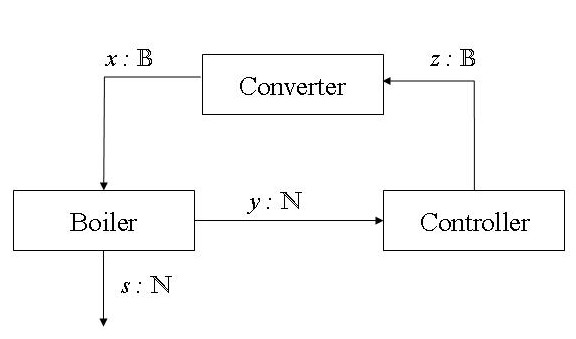
\includegraphics[width=7cm]{fig/BoilerSystemArch.jpg}
\end{spec}
}

The  \emph{SteamBoiler}  component works in time-synchronous manner: 
the current water level is controlled every time interval.
The boiler has two output channels with equal streams ($y = s$) and it
 fixes the initial water level to be $500$ gallons.
For every point of time the following must be true: if the pump is off, 
the boiler consumes at most $10$ gallons of water, 
otherwise (the pump is on) at most $10$ gallons of water will be added to its water tank.

The  \emph{Converter}   component converts the asynchronous output produced by the controller
to time-synchronous input for the steam boiler. 
Initially the pump is off, 
and at every later point of time (from receiving the first instruction 
from the controller) the output will be the last input from the controller. 

The   \emph{Controller}  component, 
contrary to the steam boiler component, 
 behaves in a purely asynchronous manner to keep
the number of control signals small, it means it might not be
desirable to switch the pump on and off more often than necessary.
The controller is responsible for
switching the steam boiler pump on and off. 
% 
If the pump is off: 
if the current water level is above $300$ gallons 
the pump stays off, otherwise the pump is started 
and will run until the water level reaches $700$ gallons. 
% 
If the pump is on: if the current water level is below $700$ gallons 
the pump stays on, otherwise the pump is turned off 
and will be off until the water level reaches $300$ gallons.

To show that the specified system fulfills the requirements we need to show that
the specification \emph{ControlSystemArch} is a refinement of the specification \emph{ControlSystem}. 
It follows from the definition of behavioral refinement that in order to verify that 
$
ControlSystem~ \leadsto ~ ControlSystemArch
$
it is enough to prove that
$$
\tlangle ControlSystemArch\trangle~ \Rightarrow ~\tlangle ControlSystem\trangle
$$
% 
Therefore, we have to  prove a \emph{lemma} 
that says the specification \emph{ControlSystemArch} is a refinement of the specification \emph{ControlSystem}:\\


\begin{isabellebody}%
\isacommand{lemma}\isamarkupfalse%
\ L{\isadigit{0}}{\isacharunderscore}ControlSystem{\isacharcolon} 
{\isasymlbrakk}\ ControlSystemArch\ s{\isasymrbrakk}\ {\isasymLongrightarrow}\ ControlSystem\ s\\
\end{isabellebody}% 


%==================================================

\subsection{Case Study 2: FlexRay Communication Protocol}

In this section we present a case study on FlexRay, 
communication protocol for safety-critical real-time applications. 
This protocol has been developed by the \fr Consortium \cite{FlexRayConsortium} 
for embedded systems in vehicles, and its advantages  
are deterministic real-time message transmission, fault tolerance, 
integrated functionality for clock synchronisation and higher bandwidth.

\fr contains a set of complex algorithms to provide the communication
services. From the view of the software layers above \fr only a few 
of these properties become visible. The most important ones are static 
cyclic communication schedules and system-wide synchronous clocks. 
These provide a suitable platform for distributed control algorithms 
as used e.g.\ in drive-by-wire applications. The formalization described 
here is based on the ``Protocol Specification 2.0''\cite{FlexRayProt}.
 
The static message transmission model of \fr is based
on \textit{rounds}. \fr rounds consist of a constant number of
time slices of the same length, so called \emph{slots}.
A node can broadcast its messages to other nodes at
statically defined slots. At most one node can
do it during any slot.

For the formalisation of \fr in \Focus we would like to refer to  \cite{efts_book} and \cite{spichkova}. 
To reduce the complexity of the system several aspects of \fr have been abstracted in this formalisation:
%
\begin{itemize}
\item[(1)] There is no clock synchronization or start-up phase since clocks are assumed to be synchronous. 
This corresponds very well with the \emph{time-synchronous} notion of \Focus.
%
\item[(2)] The model does not contain bus guardians that protect channels on the physical layer from interference caused by communication that is not aligned with FlexRay schedules.
%
\item[(3)] Only the static segment of the communication cycle has been included not the dynamic, 
as we are mainly interested in time-triggered systems.
%
\item[(4)] The time-basis for the system is one slot i.e.\ one slot \fr corresponds to one tick in in the formalisation.
%
\item[(5)] The system contains only one \fr channel. Adding a second channel 
would mean simply doubling the \fr component with a different configuration 
and adding extra channels for the access to the \emph{CNI\_Buffer} component.
\end{itemize}
% 
The system architecture consists of the following components, 
which describe the \fr components accordingly to the \fr standard~\cite{FlexRayProt}: 
%
\begin{itemize*}
  \item \emph{FlexRay} (general requirements specification), 
  \item \emph{FlexRayArch} (system architecture),   
  \item \emph{FlexRayArchitecture} 
(guarantee part of the system architecture), 
  \item \emph{Cable}, 
  \item \emph{Controller}, 
  \item \emph{Scheduler}, and 
  \item \emph{BusInterface}. 
  \end{itemize*}
  % 
We present the following \isah theories in this case study:
%
\begin{itemize*}
  \item \ist{FR\_types.thy} -- datatype definitions, 
  \item \ist{FR.thy} --  specifications of the system components and auxiliary functions and predicates, 
  \item \ist{FR\_proof} --   proof of refinement relation between the requirements and the architecture specifications.
\end{itemize*}
%
The type \emph{Frame} that describes a \fr frame 
 consists of a slot identifier of type \Nat~and the payload.
The type of payload is defined as a finite list of type \emph{Message}.
  The type \emph{Config} represents the bus configuration and contains the 
scheduling table \emph{schedule} of a node and the length 
of the communication round \emph{cycleLength}. 
A scheduling table of a node consists of a number of slots 
in which this node should be sending a frame with the corresponding identifier
(identifier that is equal to the slot).
%
\[
\begin{array}{lcl}
  \ntype Message & = & msg~(message\_id: \Nat, ftcdata : Data) \\
  \ntype Frame  & = & frm~(slot : \Nat, data : Data) \\
  \ntype Config & = & conf~(schedule: \nfst{\Nat}, cycleLength: \Nat )
\end{array}
\]
%
We do not specify the type \emph{Data} here to have a polymorphic specification 
of \fr (this type can be underspecified later to any datatype), therefore, in \isah it will be also defined as a polymorphic type \ist{$'$a}. 
The types \ist{$'$a~nFrame}, \ist{nNat} and \ist{nConfig} 
are used to represent sheaves of channels of types 
\emph{Frame}, \Nat~and \emph{Config} respectively.
In the specification group will be used 
channels \emph{recv} and \emph{activations}, as well as sheaves of channels 
(\emph{return$_1$, \dots,return$_n$}), ($c_1, \dots, c_n$), 
(\emph{store}$_1$, \dots, \emph{store}$_n$), (\emph{get}$_1$, \dots, \emph{get}$_n$), and 
(\emph{send}$_1$, \dots, \emph{send}$_n$).
We also need to declare some constant, \ist{sN}, for the number of specification replication and the corresponding number of channels in sheaves, as well as to define the list of sheaf upper 
bounds, \ist{sheafNumbers}.

The architecture of the \fr communication protocol  is specified
as the \Focus specification \emph{FlexRayArch}. 
Its assumption-part consists of three constraints:
(i) all bus configurations have disjoint scheduling tables, 
(ii) all bus configurations have the equal length of the communication round,
(iii) each \fr controller can receive tab most one data frame each time interval from the environment' of the \fr system.
The guarantee-part of \emph{FlexRayArch} is represented by the specification 
\emph{FlexRayArchitecture} (see below).  
  
{\footnotesize
\begin{spec}{\spc{FlexRayArch} \fconsts}{td}
\InOut{return_1 ,..., return_n : Frame}{store_1 ,..., store_n : Frame ; get_1 ,..., get_n : \Nat}
\begin{array}{ll}
\uasm 
 &\forall i \in [1..n]: \msg{1}{return_i}\\
 &  DisjointSchedules(c_1 ,\dots, c_n)\\
 & IdenticCycleLength(c_1 ,\dots, c_n) \\
\ugar
 & (store_1 ,\dots, store_n, get_1 ,\dots, get_n) := \\
 & ~~~~~~FlexRayArchitecture(c_1 ,\dots, c_n)(return_1 ,dots, return_n)
\end{array}
\end{spec}
}


{\footnotesize
\begin{spec}{\spc{FlexRayArchitecture}\fconsts}{gb}
\centering
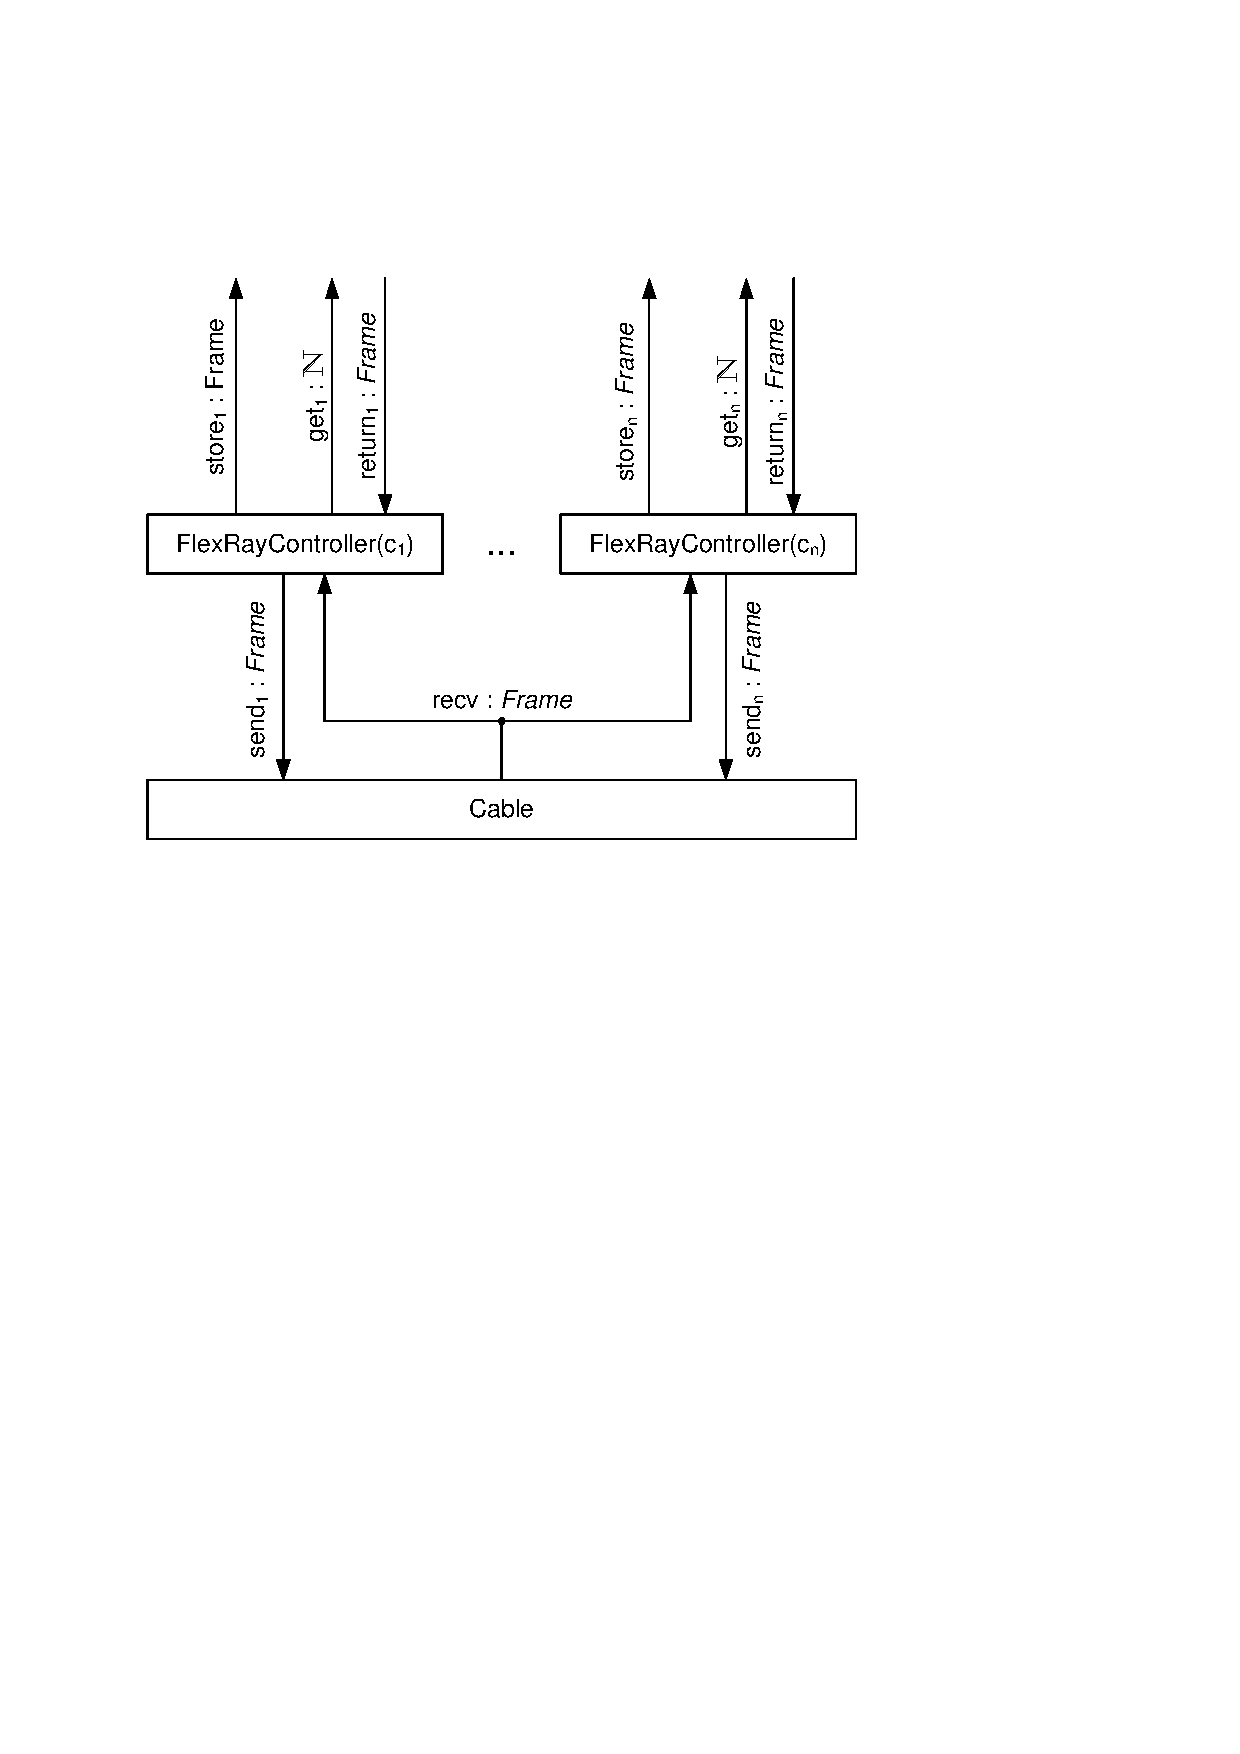
\includegraphics[width=8cm]{fig/flexray.pdf}
\end{spec}
}

\noindent
The component \emph{Cable} simulate the broadcast properties of the 
physical network cable -- 
every received \fr frame is resent to all connected nodes. 
Thus, if one \emph{FlexRayController} send some frame, 
this frame will be resent to all nodes 
(to all \emph{FlexRayController}s of the system).
The assumption is that all input streams of the component \emph{Cable} 
 are disjoint -- this holds by the properties of the 
\emph{FlexRayController} components and the overall system assumption that 
the scheduling tables of all nodes are disjoint.  
The guarantee is specified by the predicate \emph{Broadcast}. 

The \Focus specification \emph{FlexRayController} represent the controller component 
for a single node of the system. It consists of the components \emph{Scheduler} 
and \emph{BusInterface}. 
The \emph{Scheduler} signals the \emph{BusInterface}, that is responsible for 
the interaction with other nodes of the system (i.e. for the real send and receive of frames),  
on which time which \fr frames must be send from the node. 
The \emph{Scheduler} describes the communication scheduler. 
It sends at every time $t$ interval, which is equal modulo the length 
of the communication cycle to some \fr frame identifier (that corresponds to the number of the slot in the communication round) from the scheduler table, 
this frame identifier.  

%
The  specification \emph{FlexRay}  represents requirements on the protocol: 
If the scheduling tables are correct in terms of the predicates 
\emph{Disjoint\-Schedules} (all bus configurations have disjoint scheduling tables) 
and \emph{Identic\-Cycle\-Length} (all bus configurations have the equal length of the communication round), and 
also the \fr component receives in every time interval at most one message from each node 
(via channels $return_i$, $1 \le i \le n$), then
\begin{itemize}
  \item 
  the frame transmission by \fr must be correct in terms of the predicate 
  \emph{FrameTransmission}: if the time $t$ is equal modulo the length of the cycle (\fr communication round) 
to the element of the scheduler table of the node $k$, then this and only this node 
can send a data atn the $t$th time interval;
  \item 
  \fr component sends in every time interval at most one message to each node 
 via channels $get_i$ and $store_i$, $1 \le i \le n$).
\end{itemize}
%
To show that the specified system fulfill the requirements we need to show that
the specification \emph{FlexRayArch} is a refinement of the specification \emph{FlexRay}. 
It follows from the definition of behavioral refinement that in order to verify that 
$
FlexRay~ \leadsto ~ FlexRayArch
$
%
it is enough to prove that
$$
\tlangle FlexRayArch\trangle~ \Rightarrow ~\tlangle FlexRay\trangle
$$
% 
Therefore, we have to define and to prove a lemma, that says the specification 
\emph{FlexRayArch} is a refinement of the specification \emph{FlexRay}:
\\

\begin{isabellebody}%
\isacommand{lemma}\isamarkupfalse%
\ main{\isacharunderscore}fr{\isacharunderscore}refinement{\isacharcolon}\isanewline
FlexRayArch\ n\ nReturn\ nC\ nStore\ nGet\ %\isanewline
%\ \ 
{\isasymLongrightarrow}\ FlexRay\ n\ nReturn\ nC\ nStore\ nGet\isanewline
\end{isabellebody}%





%==================================================

\subsection{Case Study 3: Automotive-Gateway}


This section introduces the case study on telematics 
(electronic data transmission) gateway that was done for the 
Verisoft project\footnote{\url{http://www.verisoft.de}}. 
If the gateway receives from a ECall application of a vehicle
a signal about crash 
(more precise, the command to initiate the call to the Emergency Service Center, ESC), 
and after the establishing the connection it receives 
 the command to send the crash data, received from sensors.
These data are restored 
 in the internal buffer of the gateway  and should  
 be resent to the ESC and 
 the voice communication will be established, assuming that
  there is no connection fails.  
The system description consists of the following specifications: 
\begin{itemize*}
  \item \emph{GatewaySystem} (gateway system architecture), 
  \item \emph{GatewaySystemReq} (gateway system requirements), 
  \item \emph{ServiceCenter} (Emergency Service Center),
  \item \emph{Gateway} (gateway architecture), 
  \item \emph{GatewayReq} (gateway requirements),
  \item \emph{Sample} (the main  component describing its logic), 
  \item \emph{Delay} (the  component   modelling the communication delay), and
  \item \emph{Loss} (the  component modelling the communication loss).  
\end{itemize*}
%  
We present the following \isah theories in this case study:
\begin{itemize*}
  \item \ist{Gateway\_types.thy} --  datatype definitions, 
  \item \ist{Gateway.thy} --  specifications of the system components, 
  \item \ist{Gateway\_proof} --  proofs of refinement relations between the requirements and the architecture specifications (for the components \emph{Gateway} and \emph{GatewaySystem}).
\end{itemize*}
%
The datatype \emph{ECall\_Info} represents a tuple, 
consisting of the data that the Emergency Service Center needs -- here we specify these data to contain the vehicle coordinates and the collision speed, they can also extend by some other information.  
The datatype \emph{GatewayStatus} represents the status (internal state) of the gateway.
%
\[
\begin{array}{lcl}
  \ntype Coordinates &=& \Nat \times \Nat
  \\
  \ntype CollisionSpeed &=& \Nat
  \\
  \ntype ECall\_Info &=& ecall(coord \in Coordinates, speed \in CollisionSpeed)
  \\
  \ntype GatewayStatus &=& 
  \{~ init\_state,~ call,~ connection\_ok,\\
  && ~ ~sending\_data,~ voice\_com ~\}
\end{array}
\]
To specify the automotive gateway we will use a number of datatypes 
consisting of one or two elements: 
$\{init, send\}$, $\{stop\_vc\}$, $\{vc\_com\}$ and $\{sc\_ack\}$. 
We name these types \emph{reqType}, \emph{stopType}, \emph{vcType} and \emph{aType} correspondingly.

The \Focus specification of the general gateway system architecture is presented below:

\begin{spec}{\spc{GatewaySystem}(\nconst d \in \Nat)}{gb}
\centering 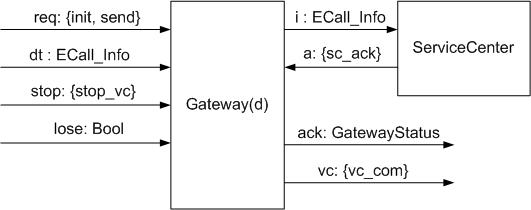
\includegraphics[width=7cm]{fig/gatewaySystem.jpg}
\end{spec} 

\noindent
The stream \emph{loss} is specified to be a time-synchronous one (exactly one message each time interval). 
It represents the connection status: 
the message \ntrue~at the time interval $t$ corresponds to the connection 
failure at this time interval, the message \nfalse~at the time interval $t$ means that 
at this time interval no data loss on the gateway connection.

The specification \emph{GatewaySystemReq} specifies the requirements for the component \emph{GatewaySystem}:
Assuming that the input streams \emph{req} and \emph{stop} can contain at every time interval at most one message, and assuming that the stream \emph{lose} contains at every time interval exactly one message. 
If 
\begin{itemize*}
  \item 
  at any time interval $t$ the gateway system is in the initial state, 
  \item
  at time interval $t+1$ the signal about crash comes at first time 
  (more precise, the command to initiate the call to the ESC,
  \item 
  after $3+m$ time intervals the command to send the crash data comes at first time,
  \item 
  the gateway system has received until the time interval $t+2$ the crash data,  
  \item 
  there is no connection fails from the time interval $t$ until the time interval $t + 4 + k + 2d$,
  \end{itemize*}
%
then at time interval $t + 4 + k + 2d$ the voice communication is established.


The component \emph{ServiceCenter} represents the interface behaviour of the ESC 
(wrt. connection to the gateway): 
if at time $t$ a message about a vehicle crash comes, it acknowledges this event by sending 
the at time $t+1$ message \emph{sc\_ack} that represents the 
attempt to establish the voice communication with the driver or a passenger of the vehicle. 
if there is no connection failure, after $d$ time intervals the voice communication will be started. 

We specify the gateway requirements (\emph{GatewayReq}) as follows: 
  \begin{enumerate}
  \item 
  %1
  If at time $t$ the gateway is in the initial state $init\_state$, and it gets 
  the command to establish the connection with the central station, and also there is no 
  environment connection problems during the next 2 time intervals, 
  it establishes the connection at the time interval $t+2$. 
  \item 
  %2
  If at time $t$  the gateway has establish the connection, 
  and it gets the command to send the ECall data to the central station, and also there is no 
  environment connection problems during the next $d+1$ time intervals, 
  then it sends the last corresponding data. 
        The central station becomes these date at the time $t+d$.
  % 
  \item 
  %3
  If the gateway becomes the acknowledgment from the central station 
  that it has receives the sent ECall data, and also there is no 
  environment connection problems, then the voice communication is started.
  \end{enumerate}
 %
 The specification of the gateway architecture, \emph{Gateway}, is parameterised one: 
the parameter $d \in \Nat$ denotes the communication delay 
between the central station and a vehicle. 
This component consists of three subcomponents: \emph{Sample}, \emph{Delay}, 
and \emph{Loss}: 
 
\begin{spec}{\spc{Gateway}(\nconst d \in \Nat)}{td}
\centering 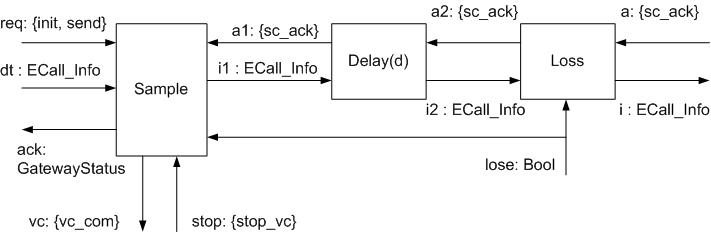
\includegraphics[width=10cm]{fig/gateway.jpg}
\end{spec} 
  
\noindent
The component \emph{Delay} models the communication delay. 
Its specification is parameterised one: 
it inherits the parameter of the component \emph{Gateway}. 
This component simply delays all input messages on $d$ time intervals. 
During the first $d$ time intervals no output message will be produced. 

The component \emph{Loss} models the communication loss between 
the central station and the vehicle gateway: 
if during time interval $t$ from the component \emph{Loss} no message about a 
lost connection comes, the messages come during time interval 
$t$ via the input channels $a$ and $i2$ will be forwarded without any delay via channels 
$a2$ and $i$ respectively. 
Otherwise all messages come during time interval 
$t$ will be lost.  
  
The component \emph{Sample} represents the logic of the gateway component. 
If it receives from a ECall application of a vehicle 
 the command to initiate the call to the ESC it tries 
 to establish the connection.
If the connection is established, and the component \emph{Sample} receives 
from a ECall application of a vehicle
 the command to send the crash data, which were already received and stored 
 in the internal buffer of the gateway, 
 these data will be resent to the ESC. 
 After that this component waits to the acknowledgment from the ESC. 
 If the acknowledgment is received, the voice communication will be established, assuming that
  there is no connection fails.

For the component \emph{Sample} we have the assumption, that the 
streams $req$, $a1$, and $stop$ can contain at every time interval at most one message, 
and also that the stream $loss$ must contain at every time interval exactly one message. 
This component uses local variables \emph{st} and \emph{buffer} (more precisely, 
a local variable \emph{buffer} and a state variable \emph{st}). 
The guarantee part of  the component \emph{Sample} can be specified as a timed state transition diagram  (TSTS) 
and an expression which says how the local variable 
\emph{buffer} is computed, or using the corresponding table representation, which is semantically equivalent to the TSTD.  
  
  
 \begin{figure}[h]
  \begin{center}
    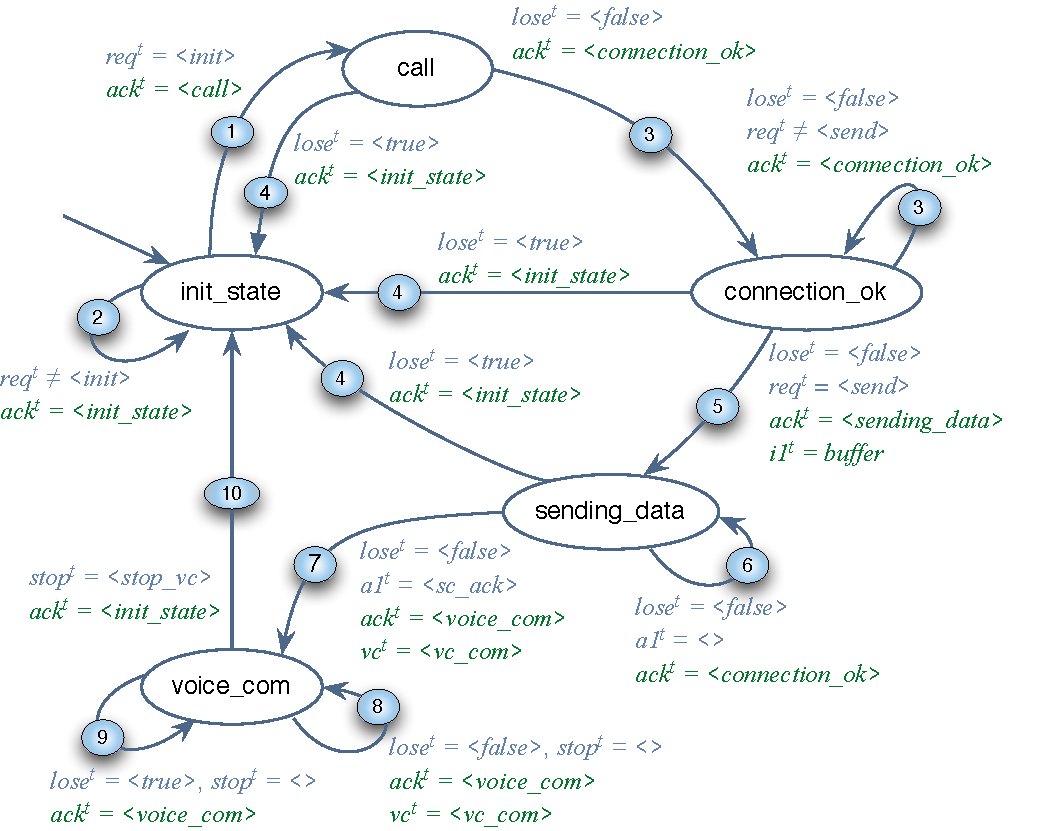
\includegraphics[scale=0.6]{fig/gatewayTSTD.pdf}
  \end{center}
  \caption{Timed state transition diagram for the component Sample}
  \label{fig:gateway_std}
\end{figure} 


  To show that the specified gateway architecture fulfils the requirements we need to show that
the specification \emph{Gateway} is a refinement of the specification \emph{GatewayReq}. 
Therefore, we need to define and to prove the following lemma:
\\

\begin{isabellebody}%
\isacommand{lemma}\isamarkupfalse%
\ Gateway{\isacharunderscore}L{\isadigit{0}}{\isacharcolon}\isanewline
\ Gateway\ req\ dt\ a\ stop\ lose\ d\ ack\ i\ vc\isanewline
\ {\isasymLongrightarrow} 
\ GatewayReq\ req\ dt\ a\ stop\ lose\ d\ ack\ i\ vc
\end{isabellebody}%

~\\
To show that the specified gateway architecture fulfills the requirements we need to show that
the specification \emph{GatewaySystem} is a refinement of the specification \emph{GatewaySystemReq}. 
Therefore, we need to define and to prove the following lemma:
\\

\begin{isabellebody}%
\isacommand{lemma}\isamarkupfalse%
\ GatewaySystem{\isacharunderscore}L{\isadigit{0}}{\isacharcolon}\isanewline
\ GatewaySystem\ req\ dt\ stop\ lose\ d\ ack\ vc\isanewline
\ {\isasymLongrightarrow} 
\ GatewaySystemReq\ req\ dt\ stop\ lose\ d\ ack\ vc\isanewline
\end{isabellebody}%  
  
%

% generated text of all theories
\input{ListExtras.tex}

%
\begin{isabellebody}%
\def\isabellecontext{Secrecy{\isacharunderscore}types}%
%
\isamarkupheader{Auxiliary data types%
}
\isamarkuptrue%
%
\isadelimtheory
%
\endisadelimtheory
%
\isatagtheory
\isacommand{theory}\isamarkupfalse%
\ Secrecy{\isacharunderscore}types\isanewline
\isakeyword{imports}\ Main\isanewline
\isakeyword{begin}\isanewline
\isanewline
%
\isamarkupcmt{We assume disjoint sets: Data of data values,%
}
\isanewline
%
\isamarkupcmt{Secrets of unguessable values, Keys - set of cryptographic  keys.%
}
\ \ \isanewline
%
\isamarkupcmt{Based on these sets, we specify the sets EncType of encryptors that may be%
}
\isanewline
%
\isamarkupcmt{used for encryption or decryption, and Expression of expression items.%
}
\isanewline
%
\isamarkupcmt{The specification (component) identifiers should be listed in the set specID,%
}
\isanewline
%
\isamarkupcmt{the channel indentifiers should be listed in the set chanID.%
}
%
\endisatagtheory
{\isafoldtheory}%
%
\isadelimtheory
%
\endisadelimtheory
\ \isanewline
\isanewline
\isacommand{datatype}\isamarkupfalse%
\ Keys\ {\isacharequal}\ CKey\ {\isacharbar}\ CKeyP\ {\isacharbar}\ SKey\ {\isacharbar}\ SKeyP\ {\isacharbar}\ genKey\ \isanewline
\isacommand{datatype}\isamarkupfalse%
\ Secrets\ {\isacharequal}\ secretD\ {\isacharbar}\ N\ {\isacharbar}\ NA\isanewline
\isacommand{type{\isacharunderscore}synonym}\isamarkupfalse%
\ Var\ \ {\isacharequal}\ {\isachardoublequoteopen}nat{\isachardoublequoteclose}\isanewline
\isacommand{type{\isacharunderscore}synonym}\isamarkupfalse%
\ Data\ {\isacharequal}\ {\isachardoublequoteopen}nat{\isachardoublequoteclose}\isanewline
\isacommand{datatype}\isamarkupfalse%
\ KS\ \ \ \ \ \ \ \ \ \ {\isacharequal}\ kKS\ Keys\ {\isacharbar}\ sKS\ Secrets\isanewline
\isacommand{datatype}\isamarkupfalse%
\ EncType\ \ {\isacharequal}\ kEnc\ Keys\ {\isacharbar}\ vEnc\ Var\isanewline
\isacommand{datatype}\isamarkupfalse%
\ specID\ {\isacharequal}\ sComp{\isadigit{1}}\ {\isacharbar}\ sComp{\isadigit{2}}\ {\isacharbar}\ sComp{\isadigit{3}}\ {\isacharbar}\ sComp{\isadigit{4}}\isanewline
\isacommand{datatype}\isamarkupfalse%
\ Expression\ {\isacharequal}\ kE\ Keys\ {\isacharbar}\ sE\ Secrets\ {\isacharbar}\ dE\ Data\ {\isacharbar}\ idE\ specID\ \isanewline
\isacommand{datatype}\isamarkupfalse%
\ chanID\ {\isacharequal}\ ch{\isadigit{1}}\ {\isacharbar}\ ch{\isadigit{2}}\ \ \ {\isacharbar}\ ch{\isadigit{3}}\ \ {\isacharbar}\ ch{\isadigit{4}}\isanewline
\isanewline
\isacommand{primrec}\isamarkupfalse%
\ Expression{\isadigit{2}}KSL{\isacharcolon}{\isacharcolon}\ {\isachardoublequoteopen}Expression\ list\ {\isasymRightarrow}\ KS\ list{\isachardoublequoteclose}\ \isanewline
\isakeyword{where}\isanewline
\ \ \ {\isachardoublequoteopen}Expression{\isadigit{2}}KSL\ {\isacharbrackleft}{\isacharbrackright}\ {\isacharequal}\ {\isacharbrackleft}{\isacharbrackright}{\isachardoublequoteclose}\ {\isacharbar}\isanewline
\ \ \ {\isachardoublequoteopen}Expression{\isadigit{2}}KSL\ {\isacharparenleft}x{\isacharhash}xs{\isacharparenright}\ {\isacharequal}\ \isanewline
\ \ \ \ \ {\isacharparenleft}{\isacharparenleft}case\ x\ of\ {\isacharparenleft}kE\ m{\isacharparenright}\ {\isasymRightarrow}\ {\isacharbrackleft}kKS\ m{\isacharbrackright}\ \isanewline
\ \ \ \ \ \ \ \ \ \ \ \ \ \ \ \ \ \ {\isacharbar}\ {\isacharparenleft}sE\ m{\isacharparenright}\ {\isasymRightarrow}\ {\isacharbrackleft}sKS\ m{\isacharbrackright}\ \isanewline
\ \ \ \ \ \ \ \ \ \ \ \ \ \ \ \ \ \ {\isacharbar}\ {\isacharparenleft}dE\ m{\isacharparenright}\ {\isasymRightarrow}\ {\isacharbrackleft}{\isacharbrackright}\ \isanewline
\ \ \ \ \ \ \ \ \ \ \ \ \ \ \ \ \ \ {\isacharbar}\ {\isacharparenleft}idE\ m{\isacharparenright}\ {\isasymRightarrow}\ {\isacharbrackleft}{\isacharbrackright}{\isacharparenright}\ {\isacharat}\ Expression{\isadigit{2}}KSL\ xs{\isacharparenright}\ {\isachardoublequoteclose}\isanewline
\isanewline
\isacommand{primrec}\isamarkupfalse%
\ KS{\isadigit{2}}Expression{\isacharcolon}{\isacharcolon}\ {\isachardoublequoteopen}KS\ {\isasymRightarrow}\ Expression{\isachardoublequoteclose}\ \isanewline
\isakeyword{where}\isanewline
\ \ {\isachardoublequoteopen}KS{\isadigit{2}}Expression\ {\isacharparenleft}kKS\ m{\isacharparenright}\ {\isacharequal}\ {\isacharparenleft}kE\ m{\isacharparenright}{\isachardoublequoteclose}\ \ {\isacharbar}\isanewline
\ \ {\isachardoublequoteopen}KS{\isadigit{2}}Expression\ {\isacharparenleft}sKS\ m{\isacharparenright}\ {\isacharequal}\ {\isacharparenleft}sE\ m{\isacharparenright}{\isachardoublequoteclose}\isanewline
%
\isadelimtheory
\isanewline
%
\endisadelimtheory
%
\isatagtheory
\isacommand{end}\isamarkupfalse%
%
\endisatagtheory
{\isafoldtheory}%
%
\isadelimtheory
%
\endisadelimtheory
\end{isabellebody}%
%%% Local Variables:
%%% mode: latex
%%% TeX-master: "root"
%%% End:


%
\begin{isabellebody}%
\def\isabellecontext{inout}%
%
\isamarkupheader{Correctness of the relations between sets of Input/Output channels%
}
\isamarkuptrue%
%
\isadelimtheory
%
\endisadelimtheory
%
\isatagtheory
\isacommand{theory}\isamarkupfalse%
\ \ inout\ \isanewline
\isakeyword{imports}\ Secrecy{\isacharunderscore}types\isanewline
\isakeyword{begin}%
\endisatagtheory
{\isafoldtheory}%
%
\isadelimtheory
%
\endisadelimtheory
\isanewline
\isanewline
\isacommand{consts}\isamarkupfalse%
\ \isanewline
\ \ subcomponents\ {\isacharcolon}{\isacharcolon}\ \ {\isachardoublequoteopen}specID\ {\isasymRightarrow}\ specID\ set{\isachardoublequoteclose}\isanewline
\isanewline
%
\isamarkupcmt{Mappings, defining sets of input, local, and output channels%
}
\isanewline
%
\isamarkupcmt{of a component%
}
\isanewline
\isacommand{consts}\isamarkupfalse%
\isanewline
\ \ ins\ {\isacharcolon}{\isacharcolon}\ {\isachardoublequoteopen}specID\ {\isasymRightarrow}\ chanID\ set{\isachardoublequoteclose}\isanewline
\ \ loc\ {\isacharcolon}{\isacharcolon}\ {\isachardoublequoteopen}specID\ {\isasymRightarrow}\ chanID\ set{\isachardoublequoteclose}\isanewline
\ \ out\ {\isacharcolon}{\isacharcolon}\ {\isachardoublequoteopen}specID\ {\isasymRightarrow}\ chanID\ set{\isachardoublequoteclose}\isanewline
\isanewline
%
\isamarkupcmt{Predicate insuring the correct mapping from the component identifier%
}
\isanewline
%
\isamarkupcmt{to the set of input channels of a component%
}
\isanewline
\isacommand{definition}\isamarkupfalse%
\isanewline
\ \ inStream\ {\isacharcolon}{\isacharcolon}\ {\isachardoublequoteopen}specID\ {\isasymRightarrow}\ chanID\ set\ {\isasymRightarrow}\ bool{\isachardoublequoteclose}\isanewline
\isakeyword{where}\isanewline
\ \ {\isachardoublequoteopen}inStream\ x\ y\ \ {\isasymequiv}\ {\isacharparenleft}ins\ x\ {\isacharequal}\ y{\isacharparenright}{\isachardoublequoteclose}\isanewline
\isanewline
%
\isamarkupcmt{Predicate insuring the correct mapping from the component identifier%
}
\isanewline
%
\isamarkupcmt{to the set of local channels of a component%
}
\isanewline
\isacommand{definition}\isamarkupfalse%
\isanewline
\ \ locStream\ {\isacharcolon}{\isacharcolon}\ {\isachardoublequoteopen}specID\ {\isasymRightarrow}\ chanID\ set\ {\isasymRightarrow}\ bool{\isachardoublequoteclose}\isanewline
\isakeyword{where}\isanewline
\ \ {\isachardoublequoteopen}locStream\ x\ y\ {\isasymequiv}\ {\isacharparenleft}loc\ x\ {\isacharequal}\ y{\isacharparenright}{\isachardoublequoteclose}\isanewline
\isanewline
%
\isamarkupcmt{Predicate insuring the correct mapping from the component identifier%
}
\isanewline
%
\isamarkupcmt{to the set of output channels of a component%
}
\isanewline
\isacommand{definition}\isamarkupfalse%
\isanewline
\ \ outStream\ {\isacharcolon}{\isacharcolon}\ {\isachardoublequoteopen}specID\ {\isasymRightarrow}\ chanID\ set\ {\isasymRightarrow}\ bool{\isachardoublequoteclose}\isanewline
\isakeyword{where}\isanewline
\ \ {\isachardoublequoteopen}outStream\ x\ y\ {\isasymequiv}\ {\isacharparenleft}out\ x\ {\isacharequal}\ y{\isacharparenright}{\isachardoublequoteclose}\isanewline
\isanewline
%
\isamarkupcmt{Predicate insuring the correct relations between%
}
\isanewline
%
\isamarkupcmt{to the set of input, output and local channels of a component%
}
\isanewline
\isacommand{definition}\isamarkupfalse%
\isanewline
\ \ correctInOutLoc\ {\isacharcolon}{\isacharcolon}\ {\isachardoublequoteopen}specID\ {\isasymRightarrow}\ bool{\isachardoublequoteclose}\isanewline
\isakeyword{where}\isanewline
\ \ {\isachardoublequoteopen}correctInOutLoc\ x\ {\isasymequiv}\ \isanewline
\ \ \ {\isacharparenleft}ins\ x{\isacharparenright}\ {\isasyminter}\ {\isacharparenleft}out\ x{\isacharparenright}\ {\isacharequal}\ {\isacharbraceleft}{\isacharbraceright}\ \isanewline
\ \ \ \ {\isasymand}\ {\isacharparenleft}ins\ x{\isacharparenright}\ {\isasyminter}\ {\isacharparenleft}loc\ x{\isacharparenright}\ {\isacharequal}\ {\isacharbraceleft}{\isacharbraceright}\ \isanewline
\ \ \ \ {\isasymand}\ {\isacharparenleft}loc\ x{\isacharparenright}\ {\isasyminter}\ {\isacharparenleft}out\ x{\isacharparenright}\ {\isacharequal}\ {\isacharbraceleft}{\isacharbraceright}\ {\isachardoublequoteclose}\ \isanewline
\isanewline
%
\isamarkupcmt{Predicate insuring the correct relations between%
}
\isanewline
%
\isamarkupcmt{sets of input channels within a composed component%
}
\isanewline
\isacommand{definition}\isamarkupfalse%
\isanewline
\ \ correctCompositionIn\ {\isacharcolon}{\isacharcolon}\ {\isachardoublequoteopen}specID\ {\isasymRightarrow}\ bool{\isachardoublequoteclose}\isanewline
\isakeyword{where}\isanewline
\ \ {\isachardoublequoteopen}correctCompositionIn\ x\ {\isasymequiv}\ \isanewline
\ \ {\isacharparenleft}ins\ x{\isacharparenright}\ {\isacharequal}\ {\isacharparenleft}{\isasymUnion}\ {\isacharparenleft}ins\ {\isacharbackquote}\ {\isacharparenleft}subcomponents\ x{\isacharparenright}{\isacharparenright}\ {\isacharminus}\ {\isacharparenleft}loc\ x{\isacharparenright}{\isacharparenright}\isanewline
\ \ {\isasymand}\ {\isacharparenleft}ins\ x{\isacharparenright}\ {\isasyminter}\ {\isacharparenleft}{\isasymUnion}\ {\isacharparenleft}out\ {\isacharbackquote}\ {\isacharparenleft}subcomponents\ x{\isacharparenright}{\isacharparenright}{\isacharparenright}\ {\isacharequal}\ {\isacharbraceleft}{\isacharbraceright}{\isachardoublequoteclose}\ \isanewline
\isanewline
%
\isamarkupcmt{Predicate insuring the correct relations between%
}
\isanewline
%
\isamarkupcmt{sets of output channels within a composed component%
}
\isanewline
\isacommand{definition}\isamarkupfalse%
\isanewline
\ \ correctCompositionOut\ {\isacharcolon}{\isacharcolon}\ {\isachardoublequoteopen}specID\ {\isasymRightarrow}\ bool{\isachardoublequoteclose}\isanewline
\isakeyword{where}\isanewline
\ \ {\isachardoublequoteopen}correctCompositionOut\ x\ {\isasymequiv}\ \isanewline
\ \ {\isacharparenleft}out\ x{\isacharparenright}\ {\isacharequal}\ {\isacharparenleft}{\isasymUnion}\ {\isacharparenleft}out\ {\isacharbackquote}\ {\isacharparenleft}subcomponents\ x{\isacharparenright}{\isacharparenright}{\isacharminus}\ {\isacharparenleft}loc\ x{\isacharparenright}{\isacharparenright}\isanewline
\ \ {\isasymand}\ {\isacharparenleft}out\ x{\isacharparenright}\ {\isasyminter}\ {\isacharparenleft}{\isasymUnion}\ {\isacharparenleft}ins\ {\isacharbackquote}\ {\isacharparenleft}subcomponents\ x{\isacharparenright}{\isacharparenright}{\isacharparenright}\ {\isacharequal}\ {\isacharbraceleft}{\isacharbraceright}\ {\isachardoublequoteclose}\ \isanewline
\isanewline
%
\isamarkupcmt{Predicate insuring the correct relations between%
}
\isanewline
%
\isamarkupcmt{sets of local channels within a composed component%
}
\isanewline
\isacommand{definition}\isamarkupfalse%
\isanewline
\ \ correctCompositionLoc\ {\isacharcolon}{\isacharcolon}\ {\isachardoublequoteopen}specID\ {\isasymRightarrow}\ bool{\isachardoublequoteclose}\isanewline
\isakeyword{where}\isanewline
\ \ {\isachardoublequoteopen}correctCompositionLoc\ x\ {\isasymequiv}\ \isanewline
\ \ \ {\isacharparenleft}loc\ x{\isacharparenright}\ {\isacharequal}\ {\isasymUnion}\ {\isacharparenleft}ins\ {\isacharbackquote}\ {\isacharparenleft}subcomponents\ x{\isacharparenright}{\isacharparenright}\isanewline
\ \ \ \ \ \ \ \ \ \ \ {\isasyminter}\ {\isasymUnion}\ {\isacharparenleft}out\ {\isacharbackquote}\ {\isacharparenleft}subcomponents\ x{\isacharparenright}{\isacharparenright}{\isachardoublequoteclose}\ \isanewline
\isanewline
%
\isamarkupcmt{If a component is an elementary one (has no subcomponents)%
}
\isanewline
%
\isamarkupcmt{its set of local channels should be empty%
}
\isanewline
\isacommand{lemma}\isamarkupfalse%
\ subcomponents{\isacharunderscore}loc{\isacharcolon}\isanewline
\isakeyword{assumes}\ {\isachardoublequoteopen}correctCompositionLoc\ x{\isachardoublequoteclose}\isanewline
\ \ \ \ \ \ \ \isakeyword{and}\ {\isachardoublequoteopen}subcomponents\ x\ {\isacharequal}\ {\isacharbraceleft}{\isacharbraceright}{\isachardoublequoteclose}\isanewline
\isakeyword{shows}\ {\isachardoublequoteopen}loc\ x\ {\isacharequal}\ {\isacharbraceleft}{\isacharbraceright}{\isachardoublequoteclose}\isanewline
%
\isadelimproof
%
\endisadelimproof
%
\isatagproof
\isacommand{using}\isamarkupfalse%
\ assms\ \isacommand{by}\isamarkupfalse%
\ {\isacharparenleft}simp\ add{\isacharcolon}\ correctCompositionLoc{\isacharunderscore}def{\isacharparenright}%
\endisatagproof
{\isafoldproof}%
%
\isadelimproof
\isanewline
%
\endisadelimproof
%
\isadelimtheory
\isanewline
%
\endisadelimtheory
%
\isatagtheory
\isacommand{end}\isamarkupfalse%
%
\endisatagtheory
{\isafoldtheory}%
%
\isadelimtheory
%
\endisadelimtheory
\end{isabellebody}%
%%% Local Variables:
%%% mode: latex
%%% TeX-master: "root"
%%% End:


%
\begin{isabellebody}%
\def\isabellecontext{Secrecy}%
%
\isamarkupheader{Secrecy: Definitions and properties%
}
\isamarkuptrue%
%
\isadelimtheory
%
\endisadelimtheory
%
\isatagtheory
\isacommand{theory}\isamarkupfalse%
\ Secrecy\isanewline
\isakeyword{imports}\ Secrecy{\isacharunderscore}types\ inout\ ListExtras\isanewline
\isakeyword{begin}\isanewline
\isanewline
%
\isamarkupcmt{Encryption, decryption, signature creation and signature verification functions%
}
\isanewline
%
\isamarkupcmt{For these functions we define only their signatures and general axioms,%
}
\isanewline
%
\isamarkupcmt{because in order to reason effectively, we view them as abstract functions and%
}
\isanewline
%
\isamarkupcmt{abstract from their implementation details%
}
%
\endisatagtheory
{\isafoldtheory}%
%
\isadelimtheory
%
\endisadelimtheory
\ \isanewline
\isacommand{consts}\isamarkupfalse%
\ \isanewline
\ \ Enc\ \ {\isacharcolon}{\isacharcolon}\ {\isachardoublequoteopen}Keys\ {\isasymRightarrow}\ Expression\ list\ {\isasymRightarrow}\ Expression\ list{\isachardoublequoteclose}\isanewline
\ \ Decr\ {\isacharcolon}{\isacharcolon}\ {\isachardoublequoteopen}Keys\ {\isasymRightarrow}\ Expression\ list\ {\isasymRightarrow}\ Expression\ list{\isachardoublequoteclose}\isanewline
\ \ Sign\ {\isacharcolon}{\isacharcolon}\ {\isachardoublequoteopen}Keys\ {\isasymRightarrow}\ Expression\ list\ {\isasymRightarrow}\ Expression\ list{\isachardoublequoteclose}\isanewline
\ \ Ext\ \ \ {\isacharcolon}{\isacharcolon}\ {\isachardoublequoteopen}Keys\ {\isasymRightarrow}\ Expression\ list\ {\isasymRightarrow}\ Expression\ list{\isachardoublequoteclose}\isanewline
\isanewline
%
\isamarkupcmt{Axioms on relations between encription and decription keys%
}
\isanewline
\isacommand{axiomatization}\isamarkupfalse%
\isanewline
\ \ \ EncrDecrKeys\ {\isacharcolon}{\isacharcolon}\ {\isachardoublequoteopen}Keys\ \ {\isasymRightarrow}\ Keys\ {\isasymRightarrow}\ bool{\isachardoublequoteclose}\isanewline
\isakeyword{where}\isanewline
ExtSign{\isacharcolon}\ \isanewline
\ {\isachardoublequoteopen}EncrDecrKeys\ K{\isadigit{1}}\ K{\isadigit{2}}\ {\isasymlongrightarrow}\ {\isacharparenleft}Ext\ K{\isadigit{1}}\ {\isacharparenleft}Sign\ K{\isadigit{2}}\ E{\isacharparenright}{\isacharparenright}\ {\isacharequal}\ E{\isachardoublequoteclose}\ \ \isakeyword{and}\isanewline
DecrEnc{\isacharcolon}\isanewline
\ {\isachardoublequoteopen}EncrDecrKeys\ K{\isadigit{1}}\ K{\isadigit{2}}\ {\isasymlongrightarrow}\ {\isacharparenleft}Decr\ K{\isadigit{2}}\ {\isacharparenleft}Enc\ K{\isadigit{1}}\ E{\isacharparenright}{\isacharparenright}\ {\isacharequal}\ E{\isachardoublequoteclose}\isanewline
\isanewline
%
\isamarkupcmt{Set of private keys of a component%
}
\isanewline
\isacommand{consts}\isamarkupfalse%
\isanewline
\ specKeys\ {\isacharcolon}{\isacharcolon}\ {\isachardoublequoteopen}specID\ {\isasymRightarrow}\ Keys\ set{\isachardoublequoteclose}\isanewline
%
\isamarkupcmt{Set of unguessable values used by a component%
}
\isanewline
\isacommand{consts}\isamarkupfalse%
\ \isanewline
\ specSecrets\ {\isacharcolon}{\isacharcolon}\ {\isachardoublequoteopen}specID\ {\isasymRightarrow}\ Secrets\ set{\isachardoublequoteclose}\isanewline
\isanewline
%
\isamarkupcmt{Join set of private keys and unguessable values used by a component%
}
\isanewline
\isacommand{definition}\isamarkupfalse%
\isanewline
\ \ specKeysSecrets\ {\isacharcolon}{\isacharcolon}\ {\isachardoublequoteopen}specID\ {\isasymRightarrow}\ KS\ set{\isachardoublequoteclose}\isanewline
\isakeyword{where}\isanewline
\ {\isachardoublequoteopen}specKeysSecrets\ C\ {\isasymequiv}\isanewline
\ \ {\isacharbraceleft}y\ {\isachardot}\ \ {\isasymexists}\ x{\isachardot}\ y\ {\isacharequal}\ {\isacharparenleft}kKS\ x{\isacharparenright}\ \ {\isasymand}\ {\isacharparenleft}x\ {\isasymin}\ {\isacharparenleft}specKeys\ C{\isacharparenright}{\isacharparenright}{\isacharbraceright}\ {\isasymunion}\isanewline
\ \ {\isacharbraceleft}z\ {\isachardot}\ \ {\isasymexists}\ s{\isachardot}\ z\ {\isacharequal}\ {\isacharparenleft}sKS\ s{\isacharparenright}\ \ {\isasymand}\ {\isacharparenleft}s\ {\isasymin}\ {\isacharparenleft}specSecrets\ C{\isacharparenright}{\isacharparenright}{\isacharbraceright}{\isachardoublequoteclose}\isanewline
\isanewline
%
\isamarkupcmt{Predicate defining that a list of expression items does not contain%
}
\isanewline
%
\isamarkupcmt{any private key  or unguessable value used by a component%
}
\isanewline
\isacommand{definition}\isamarkupfalse%
\isanewline
\ \ notSpecKeysSecretsExpr\ {\isacharcolon}{\isacharcolon}\ {\isachardoublequoteopen}specID\ {\isasymRightarrow}\ \ Expression\ list\ {\isasymRightarrow}\ bool{\isachardoublequoteclose}\isanewline
\isakeyword{where}\isanewline
\ \ \ \ \ {\isachardoublequoteopen}notSpecKeysSecretsExpr\ P\ e\ {\isasymequiv}\isanewline
\ \ \ \ \ {\isacharparenleft}{\isasymforall}\ x{\isachardot}\ {\isacharparenleft}kE\ x{\isacharparenright}\ mem\ e\ {\isasymlongrightarrow}\ {\isacharparenleft}kKS\ x{\isacharparenright}\ {\isasymnotin}\ specKeysSecrets\ P{\isacharparenright}\ {\isasymand}\isanewline
\ \ \ \ \ {\isacharparenleft}{\isasymforall}\ y{\isachardot}\ {\isacharparenleft}sE\ y{\isacharparenright}\ mem\ e\ {\isasymlongrightarrow}\ {\isacharparenleft}sKS\ y{\isacharparenright}\ {\isasymnotin}\ specKeysSecrets\ P{\isacharparenright}{\isachardoublequoteclose}\isanewline
\isanewline
%
\isamarkupcmt{If a component is a composite one, the set of its private keys%
}
\ \isanewline
%
\isamarkupcmt{is a union of the subcomponents' sets of the private keys%
}
\isanewline
\isacommand{definition}\isamarkupfalse%
\isanewline
\ \ correctCompositionKeys\ {\isacharcolon}{\isacharcolon}\ \ {\isachardoublequoteopen}specID\ {\isasymRightarrow}\ bool{\isachardoublequoteclose}\isanewline
\isakeyword{where}\isanewline
\ \ {\isachardoublequoteopen}correctCompositionKeys\ x\ {\isasymequiv}\isanewline
\ \ \ \ subcomponents\ x\ {\isasymnoteq}\ {\isacharbraceleft}{\isacharbraceright}\ {\isasymlongrightarrow}\ \isanewline
\ \ \ \ specKeys\ x\ {\isacharequal}\ \ {\isasymUnion}\ {\isacharparenleft}specKeys\ {\isacharbackquote}\ {\isacharparenleft}subcomponents\ x{\isacharparenright}{\isacharparenright}{\isachardoublequoteclose}\ \isanewline
\isanewline
%
\isamarkupcmt{If a component is a composite one, the set of its unguessable values%
}
\ \isanewline
%
\isamarkupcmt{is a union of the subcomponents' sets of the unguessable values%
}
\isanewline
\isacommand{definition}\isamarkupfalse%
\isanewline
\ \ correctCompositionSecrets\ {\isacharcolon}{\isacharcolon}\ \ {\isachardoublequoteopen}specID\ {\isasymRightarrow}\ bool{\isachardoublequoteclose}\isanewline
\isakeyword{where}\isanewline
\ \ {\isachardoublequoteopen}correctCompositionSecrets\ x\ {\isasymequiv}\isanewline
\ \ \ \ subcomponents\ x\ {\isasymnoteq}\ {\isacharbraceleft}{\isacharbraceright}\ {\isasymlongrightarrow}\ \isanewline
\ \ \ \ specSecrets\ x\ {\isacharequal}\ \ {\isasymUnion}\ {\isacharparenleft}specSecrets\ {\isacharbackquote}\ {\isacharparenleft}subcomponents\ x{\isacharparenright}{\isacharparenright}{\isachardoublequoteclose}\ \isanewline
\isanewline
%
\isamarkupcmt{If a component is a composite one, the set of its private keys and%
}
\ \isanewline
%
\isamarkupcmt{unguessable values is a union of the corresponding sets of its subcomponents%
}
\isanewline
\isacommand{definition}\isamarkupfalse%
\isanewline
\ \ correctCompositionKS\ {\isacharcolon}{\isacharcolon}\ \ {\isachardoublequoteopen}specID\ {\isasymRightarrow}\ bool{\isachardoublequoteclose}\isanewline
\isakeyword{where}\isanewline
\ \ {\isachardoublequoteopen}correctCompositionKS\ x\ {\isasymequiv}\isanewline
\ \ \ \ subcomponents\ x\ {\isasymnoteq}\ {\isacharbraceleft}{\isacharbraceright}\ {\isasymlongrightarrow}\ \isanewline
\ \ \ \ specKeysSecrets\ x\ {\isacharequal}\ \ {\isasymUnion}\ {\isacharparenleft}specKeysSecrets\ {\isacharbackquote}\ {\isacharparenleft}subcomponents\ x{\isacharparenright}{\isacharparenright}{\isachardoublequoteclose}\ \isanewline
\isanewline
%
\isamarkupcmt{Predicate defining set of correctness properties of the component's%
}
\isanewline
%
\isamarkupcmt{interface  and relations on its private keys and unguessable values%
}
\isanewline
\isacommand{definition}\isamarkupfalse%
\isanewline
\ \ correctComponentSecrecy\ \ {\isacharcolon}{\isacharcolon}\ \ {\isachardoublequoteopen}specID\ {\isasymRightarrow}\ bool{\isachardoublequoteclose}\isanewline
\isakeyword{where}\ \isanewline
\ \ {\isachardoublequoteopen}correctComponentSecrecy\ x\ {\isasymequiv}\ \isanewline
\ \ \ \ correctCompositionKS\ x\ {\isasymand}\ \isanewline
\ \ \ \ correctCompositionSecrets\ x\ {\isasymand}\ \isanewline
\ \ \ \ correctCompositionKeys\ x\ {\isasymand}\ \isanewline
\ \ \ \ correctCompositionLoc\ x\ {\isasymand}\isanewline
\ \ \ \ correctCompositionIn\ x\ {\isasymand}\isanewline
\ \ \ \ correctCompositionOut\ x\ {\isasymand}\ \isanewline
\ \ \ \ correctInOutLoc\ x{\isachardoublequoteclose}\isanewline
\isanewline
%
\isamarkupcmt{Predicate exprChannel I E defines whether the expression item E can be sent via the channel I%
}
\ \ \ \ \isanewline
\isacommand{consts}\isamarkupfalse%
\isanewline
\ exprChannel\ {\isacharcolon}{\isacharcolon}\ {\isachardoublequoteopen}chanID\ {\isasymRightarrow}\ Expression\ {\isasymRightarrow}\ bool{\isachardoublequoteclose}\isanewline
\isanewline
%
\isamarkupcmt{Predicate eoutM sP M E defines whether the component sP may eventually%
}
\isanewline
%
\isamarkupcmt{output an expression E if there exists a time interval t of%
}
\ \isanewline
%
\isamarkupcmt{an output channel which contains this expression E%
}
\isanewline
\isacommand{definition}\isamarkupfalse%
\isanewline
\ \ eout\ {\isacharcolon}{\isacharcolon}\ {\isachardoublequoteopen}specID\ \ {\isasymRightarrow}\ Expression\ {\isasymRightarrow}\ bool{\isachardoublequoteclose}\isanewline
\isakeyword{where}\isanewline
\ {\isachardoublequoteopen}eout\ sP\ E\ {\isasymequiv}\ \isanewline
\ \ {\isasymexists}\ {\isacharparenleft}ch\ {\isacharcolon}{\isacharcolon}\ chanID{\isacharparenright}{\isachardot}\ {\isacharparenleft}{\isacharparenleft}ch\ {\isasymin}\ {\isacharparenleft}out\ sP{\isacharparenright}{\isacharparenright}\ {\isasymand}\ {\isacharparenleft}exprChannel\ ch\ E{\isacharparenright}{\isacharparenright}{\isachardoublequoteclose}\isanewline
\isanewline
%
\isamarkupcmt{Predicate eout sP E defines whether the component sP may eventually%
}
\isanewline
%
\isamarkupcmt{output an expression E via subset of channels M,%
}
\isanewline
%
\isamarkupcmt{which is a subset of output channels of sP,%
}
\isanewline
%
\isamarkupcmt{and if there exists a time interval t of%
}
\ \isanewline
%
\isamarkupcmt{an output channel which contains this expression E%
}
\isanewline
\isacommand{definition}\isamarkupfalse%
\isanewline
\ \ eoutM\ {\isacharcolon}{\isacharcolon}\ {\isachardoublequoteopen}specID\ \ {\isasymRightarrow}\ chanID\ set\ {\isasymRightarrow}\ Expression\ {\isasymRightarrow}\ bool{\isachardoublequoteclose}\isanewline
\isakeyword{where}\isanewline
\ {\isachardoublequoteopen}eoutM\ sP\ M\ E\ {\isasymequiv}\ \isanewline
\ \ {\isasymexists}\ {\isacharparenleft}ch\ {\isacharcolon}{\isacharcolon}\ chanID{\isacharparenright}{\isachardot}\ {\isacharparenleft}{\isacharparenleft}ch\ {\isasymin}\ {\isacharparenleft}out\ sP{\isacharparenright}{\isacharparenright}\ {\isasymand}\ {\isacharparenleft}ch\ {\isasymin}\ M{\isacharparenright}\ {\isasymand}\ {\isacharparenleft}exprChannel\ ch\ E{\isacharparenright}{\isacharparenright}{\isachardoublequoteclose}\isanewline
\isanewline
%
\isamarkupcmt{Predicate ineM sP M E defines whether a component sP may eventually%
}
\isanewline
%
\isamarkupcmt{get an expression E  if there exists a time interval t of%
}
\ \isanewline
%
\isamarkupcmt{an input stream  which contains this expression E%
}
\isanewline
\isacommand{definition}\isamarkupfalse%
\isanewline
\ \ ine\ {\isacharcolon}{\isacharcolon}\ {\isachardoublequoteopen}specID\ \ {\isasymRightarrow}\ Expression\ {\isasymRightarrow}\ bool{\isachardoublequoteclose}\isanewline
\isakeyword{where}\isanewline
\ {\isachardoublequoteopen}ine\ sP\ E\ {\isasymequiv}\ \isanewline
\ \ {\isasymexists}\ {\isacharparenleft}ch\ {\isacharcolon}{\isacharcolon}\ chanID{\isacharparenright}{\isachardot}\ {\isacharparenleft}{\isacharparenleft}ch\ {\isasymin}\ {\isacharparenleft}ins\ sP{\isacharparenright}{\isacharparenright}\ {\isasymand}\ {\isacharparenleft}exprChannel\ ch\ E{\isacharparenright}{\isacharparenright}{\isachardoublequoteclose}\isanewline
\isanewline
%
\isamarkupcmt{Predicate ine sP E defines whether a component sP may eventually%
}
\isanewline
%
\isamarkupcmt{get an expression E via subset of channels M,%
}
\isanewline
%
\isamarkupcmt{which is a subset of input channels of sP,%
}
\isanewline
%
\isamarkupcmt{and if there exists a time interval t of%
}
\ \isanewline
%
\isamarkupcmt{an input stream  which contains this expression E%
}
\isanewline
\isacommand{definition}\isamarkupfalse%
\isanewline
\ \ ineM\ {\isacharcolon}{\isacharcolon}\ {\isachardoublequoteopen}specID\ \ {\isasymRightarrow}\ chanID\ set\ {\isasymRightarrow}\ Expression\ {\isasymRightarrow}\ bool{\isachardoublequoteclose}\isanewline
\isakeyword{where}\isanewline
\ {\isachardoublequoteopen}ineM\ sP\ M\ E\ {\isasymequiv}\ \isanewline
\ \ {\isasymexists}\ {\isacharparenleft}ch\ {\isacharcolon}{\isacharcolon}\ chanID{\isacharparenright}{\isachardot}\ {\isacharparenleft}{\isacharparenleft}ch\ {\isasymin}\ {\isacharparenleft}ins\ sP{\isacharparenright}{\isacharparenright}\ {\isasymand}\ {\isacharparenleft}ch\ {\isasymin}\ M{\isacharparenright}\ {\isasymand}\ {\isacharparenleft}exprChannel\ ch\ E{\isacharparenright}{\isacharparenright}{\isachardoublequoteclose}\isanewline
\isanewline
%
\isamarkupcmt{This predicate defines whether an input channel ch of a component sP%
}
\isanewline
%
\isamarkupcmt{is the only one input channel of this component%
}
\isanewline
%
\isamarkupcmt{via which it may eventually output an expression E%
}
\isanewline
\isacommand{definition}\isamarkupfalse%
\isanewline
\ \ out{\isacharunderscore}exprChannelSingle\ {\isacharcolon}{\isacharcolon}\ {\isachardoublequoteopen}specID\ \ {\isasymRightarrow}\ chanID\ {\isasymRightarrow}\ Expression\ {\isasymRightarrow}\ bool{\isachardoublequoteclose}\isanewline
\isakeyword{where}\isanewline
\ {\isachardoublequoteopen}out{\isacharunderscore}exprChannelSingle\ sP\ ch\ E\ {\isasymequiv}\ \isanewline
\ \ {\isacharparenleft}ch\ {\isasymin}\ {\isacharparenleft}out\ sP{\isacharparenright}{\isacharparenright}\ {\isasymand}\ \ \isanewline
\ \ {\isacharparenleft}exprChannel\ ch\ E{\isacharparenright}\ \ {\isasymand}\isanewline
\ \ {\isacharparenleft}{\isasymforall}\ {\isacharparenleft}x\ {\isacharcolon}{\isacharcolon}\ chanID{\isacharparenright}\ {\isacharparenleft}t\ {\isacharcolon}{\isacharcolon}\ nat{\isacharparenright}{\isachardot}\ {\isacharparenleft}{\isacharparenleft}x\ {\isasymin}\ {\isacharparenleft}out\ sP{\isacharparenright}{\isacharparenright}\ {\isasymand}\ {\isacharparenleft}x\ {\isasymnoteq}\ ch{\isacharparenright}\ {\isasymlongrightarrow}\ {\isasymnot}\ exprChannel\ x\ E{\isacharparenright}{\isacharparenright}{\isachardoublequoteclose}\isanewline
\isanewline
%
\isamarkupcmt{This predicate  yields true if only the channels from the set chSet,%
}
\isanewline
%
\isamarkupcmt{which is a subset of input channels of the  component sP,%
}
\isanewline
%
\isamarkupcmt{may eventually output an expression E%
}
\isanewline
\isacommand{definition}\isamarkupfalse%
\isanewline
\ out{\isacharunderscore}exprChannelSet\ {\isacharcolon}{\isacharcolon}\ {\isachardoublequoteopen}specID\ \ {\isasymRightarrow}\ chanID\ set\ {\isasymRightarrow}\ Expression\ {\isasymRightarrow}\ bool{\isachardoublequoteclose}\isanewline
\isakeyword{where}\isanewline
\ {\isachardoublequoteopen}out{\isacharunderscore}exprChannelSet\ sP\ chSet\ E\ {\isasymequiv}\ \isanewline
\ \ \ {\isacharparenleft}{\isacharparenleft}{\isasymforall}\ {\isacharparenleft}x\ {\isacharcolon}{\isacharcolon}chanID{\isacharparenright}{\isachardot}\ {\isacharparenleft}{\isacharparenleft}x\ {\isasymin}\ chSet{\isacharparenright}\ {\isasymlongrightarrow}\ {\isacharparenleft}{\isacharparenleft}x\ {\isasymin}\ {\isacharparenleft}out\ sP{\isacharparenright}{\isacharparenright}\ {\isasymand}\ {\isacharparenleft}exprChannel\ x\ E{\isacharparenright}{\isacharparenright}{\isacharparenright}{\isacharparenright}\isanewline
\ \ \ {\isasymand}\isanewline
\ \ \ {\isacharparenleft}{\isasymforall}\ {\isacharparenleft}x\ {\isacharcolon}{\isacharcolon}\ chanID{\isacharparenright}{\isachardot}\ {\isacharparenleft}{\isacharparenleft}x\ {\isasymnotin}\ chSet{\isacharparenright}\ {\isasymand}\ {\isacharparenleft}x\ {\isasymin}\ {\isacharparenleft}out\ sP{\isacharparenright}{\isacharparenright}\ {\isasymlongrightarrow}\ {\isasymnot}\ exprChannel\ x\ E{\isacharparenright}{\isacharparenright}{\isacharparenright}{\isachardoublequoteclose}\isanewline
\isanewline
%
\isamarkupcmt{This redicate defines whether%
}
\isanewline
%
\isamarkupcmt{an input channel ch of a component sP is the only one input channel%
}
\isanewline
%
\isamarkupcmt{of this component via which it may eventually get an expression E%
}
\isanewline
\isacommand{definition}\isamarkupfalse%
\isanewline
\ ine{\isacharunderscore}exprChannelSingle\ {\isacharcolon}{\isacharcolon}\ {\isachardoublequoteopen}specID\ \ {\isasymRightarrow}\ chanID\ {\isasymRightarrow}\ Expression\ {\isasymRightarrow}\ bool{\isachardoublequoteclose}\isanewline
\isakeyword{where}\isanewline
\ {\isachardoublequoteopen}ine{\isacharunderscore}exprChannelSingle\ sP\ ch\ E\ {\isasymequiv}\ \isanewline
\ \ {\isacharparenleft}ch\ {\isasymin}\ {\isacharparenleft}ins\ sP{\isacharparenright}{\isacharparenright}\ {\isasymand}\isanewline
\ \ {\isacharparenleft}exprChannel\ ch\ E{\isacharparenright}\ \ {\isasymand}\isanewline
\ \ {\isacharparenleft}{\isasymforall}\ {\isacharparenleft}x\ {\isacharcolon}{\isacharcolon}\ chanID{\isacharparenright}\ {\isacharparenleft}t\ {\isacharcolon}{\isacharcolon}\ nat{\isacharparenright}{\isachardot}\ {\isacharparenleft}{\isacharparenleft}\ x\ {\isasymin}\ {\isacharparenleft}ins\ sP{\isacharparenright}{\isacharparenright}\ {\isasymand}\ {\isacharparenleft}x\ {\isasymnoteq}\ ch{\isacharparenright}\ {\isasymlongrightarrow}\ {\isasymnot}\ exprChannel\ x\ E{\isacharparenright}{\isacharparenright}{\isachardoublequoteclose}\isanewline
\isanewline
%
\isamarkupcmt{This predicate yields true if the component sP may eventually%
}
\isanewline
%
\isamarkupcmt{get an expression E only via the channels from the set chSet,%
}
\isanewline
%
\isamarkupcmt{which is a subset of input channels of sP%
}
\isanewline
\isacommand{definition}\isamarkupfalse%
\isanewline
\ ine{\isacharunderscore}exprChannelSet\ {\isacharcolon}{\isacharcolon}\ {\isachardoublequoteopen}specID\ \ {\isasymRightarrow}\ chanID\ set\ {\isasymRightarrow}\ Expression\ {\isasymRightarrow}\ bool{\isachardoublequoteclose}\isanewline
\isakeyword{where}\isanewline
\ {\isachardoublequoteopen}ine{\isacharunderscore}exprChannelSet\ sP\ chSet\ E\ {\isasymequiv}\ \isanewline
\ \ \ {\isacharparenleft}{\isacharparenleft}{\isasymforall}\ {\isacharparenleft}x\ {\isacharcolon}{\isacharcolon}chanID{\isacharparenright}{\isachardot}\ {\isacharparenleft}{\isacharparenleft}x\ {\isasymin}\ chSet{\isacharparenright}\ {\isasymlongrightarrow}\ {\isacharparenleft}{\isacharparenleft}x\ {\isasymin}\ {\isacharparenleft}ins\ sP{\isacharparenright}{\isacharparenright}\ {\isasymand}\ {\isacharparenleft}exprChannel\ x\ E{\isacharparenright}{\isacharparenright}{\isacharparenright}{\isacharparenright}\isanewline
\ \ \ {\isasymand}\isanewline
\ \ \ {\isacharparenleft}{\isasymforall}\ {\isacharparenleft}x\ {\isacharcolon}{\isacharcolon}\ chanID{\isacharparenright}{\isachardot}\ {\isacharparenleft}{\isacharparenleft}x\ {\isasymnotin}\ chSet{\isacharparenright}\ {\isasymand}\ {\isacharparenleft}\ x\ {\isasymin}\ {\isacharparenleft}ins\ sP{\isacharparenright}{\isacharparenright}\ {\isasymlongrightarrow}\ {\isasymnot}\ exprChannel\ x\ E{\isacharparenright}{\isacharparenright}{\isacharparenright}{\isachardoublequoteclose}\isanewline
\isanewline
%
\isamarkupcmt{If a list of expression items does not contain any private key%
}
\isanewline
%
\isamarkupcmt{or unguessable value of a component P, then the first element%
}
\ \isanewline
%
\isamarkupcmt{of the list is neither a private key nor unguessable value of P%
}
\isanewline
\isacommand{lemma}\isamarkupfalse%
\ notSpecKeysSecretsExpr{\isacharunderscore}L{\isadigit{1}}{\isacharcolon}\isanewline
\isakeyword{assumes}\ {\isachardoublequoteopen}notSpecKeysSecretsExpr\ P\ {\isacharparenleft}a\ {\isacharhash}\ l{\isacharparenright}{\isachardoublequoteclose}\isanewline
\isakeyword{shows}\ \ \ \ {\isachardoublequoteopen}notSpecKeysSecretsExpr\ P\ {\isacharbrackleft}a{\isacharbrackright}{\isachardoublequoteclose}\isanewline
%
\isadelimproof
%
\endisadelimproof
%
\isatagproof
\isacommand{using}\isamarkupfalse%
\ assms\ \isacommand{by}\isamarkupfalse%
\ {\isacharparenleft}simp\ add{\isacharcolon}\ notSpecKeysSecretsExpr{\isacharunderscore}def{\isacharparenright}\isanewline
\isanewline
%
\isamarkupcmt{If a list of expression items does not contain any private key%
}
\isanewline
%
\isamarkupcmt{or unguessable value of a component P, then this list without its first%
}
\ \isanewline
%
\isamarkupcmt{element does not contain them too%
}
%
\endisatagproof
{\isafoldproof}%
%
\isadelimproof
\isanewline
%
\endisadelimproof
\isacommand{lemma}\isamarkupfalse%
\ notSpecKeysSecretsExpr{\isacharunderscore}L{\isadigit{2}}{\isacharcolon}\isanewline
\isakeyword{assumes}\ {\isachardoublequoteopen}notSpecKeysSecretsExpr\ P\ {\isacharparenleft}a\ {\isacharhash}\ l{\isacharparenright}{\isachardoublequoteclose}\isanewline
\isakeyword{shows}\ \ \ \ {\isachardoublequoteopen}notSpecKeysSecretsExpr\ P\ l{\isachardoublequoteclose}\ \isanewline
%
\isadelimproof
%
\endisadelimproof
%
\isatagproof
\isacommand{using}\isamarkupfalse%
\ assms\ \isacommand{by}\isamarkupfalse%
\ {\isacharparenleft}simp\ add{\isacharcolon}\ notSpecKeysSecretsExpr{\isacharunderscore}def{\isacharparenright}\isanewline
\isanewline
%
\isamarkupcmt{If a channel belongs to the set of input channels of a component P%
}
\isanewline
%
\isamarkupcmt{and does not belong to the set of local channels of the compositon of P and Q%
}
\ \isanewline
%
\isamarkupcmt{then it belongs to the set of input channels of this composition%
}
%
\endisatagproof
{\isafoldproof}%
%
\isadelimproof
\isanewline
%
\endisadelimproof
\isacommand{lemma}\isamarkupfalse%
\ correctCompositionIn{\isacharunderscore}L{\isadigit{1}}{\isacharcolon}\isanewline
\isakeyword{assumes}\ {\isachardoublequoteopen}subcomponents\ PQ\ {\isacharequal}\ {\isacharbraceleft}P{\isacharcomma}Q{\isacharbraceright}{\isachardoublequoteclose}\ \isanewline
\ \ \ \ \ \ \ \isakeyword{and}\ {\isachardoublequoteopen}correctCompositionIn\ PQ{\isachardoublequoteclose}\ \isanewline
\ \ \ \ \ \ \ \isakeyword{and}\ {\isachardoublequoteopen}ch\ {\isasymnotin}\ loc\ PQ{\isachardoublequoteclose}\isanewline
\ \ \ \ \ \ \ \isakeyword{and}\ {\isachardoublequoteopen}ch\ {\isasymin}\ ins\ P{\isachardoublequoteclose}\ \isanewline
\isakeyword{shows}\ \ \ \ {\isachardoublequoteopen}ch\ {\isasymin}\ ins\ PQ{\isachardoublequoteclose}\isanewline
%
\isadelimproof
%
\endisadelimproof
%
\isatagproof
\isacommand{using}\isamarkupfalse%
\ assms\ \isacommand{by}\isamarkupfalse%
\ {\isacharparenleft}simp\ add{\isacharcolon}\ correctCompositionIn{\isacharunderscore}def{\isacharparenright}\isanewline
\isanewline
%
\isamarkupcmt{If a channel belongs to the set of input channels of the compositon of P and Q%
}
\isanewline
%
\isamarkupcmt{then it belongs to the set of input channels either of P or of Q%
}
%
\endisatagproof
{\isafoldproof}%
%
\isadelimproof
\isanewline
%
\endisadelimproof
\isacommand{lemma}\isamarkupfalse%
\ correctCompositionIn{\isacharunderscore}L{\isadigit{2}}{\isacharcolon}\isanewline
\isakeyword{assumes}\ {\isachardoublequoteopen}subcomponents\ PQ\ {\isacharequal}\ {\isacharbraceleft}P{\isacharcomma}Q{\isacharbraceright}{\isachardoublequoteclose}\isanewline
\ \ \ \ \ \ \ \isakeyword{and}\ {\isachardoublequoteopen}correctCompositionIn\ PQ{\isachardoublequoteclose}\ \isanewline
\ \ \ \ \ \ \ \isakeyword{and}\ {\isachardoublequoteopen}ch\ {\isasymin}\ ins\ PQ{\isachardoublequoteclose}\ \isanewline
\isakeyword{shows}\ \ \ \ {\isachardoublequoteopen}{\isacharparenleft}ch\ {\isasymin}\ ins\ P{\isacharparenright}\ {\isasymor}\ {\isacharparenleft}ch\ {\isasymin}\ ins\ Q{\isacharparenright}{\isachardoublequoteclose}\ \isanewline
%
\isadelimproof
%
\endisadelimproof
%
\isatagproof
\isacommand{using}\isamarkupfalse%
\ assms\ \isacommand{by}\isamarkupfalse%
\ {\isacharparenleft}simp\ add{\isacharcolon}\ correctCompositionIn{\isacharunderscore}def{\isacharparenright}%
\endisatagproof
{\isafoldproof}%
%
\isadelimproof
\isanewline
%
\endisadelimproof
\isanewline
\isacommand{lemma}\isamarkupfalse%
\ ineM{\isacharunderscore}L{\isadigit{1}}{\isacharcolon}\isanewline
\isakeyword{assumes}\ {\isachardoublequoteopen}ch\ {\isasymin}\ M{\isachardoublequoteclose}\ \isanewline
\ \ \ \ \ \ \ \isakeyword{and}\ {\isachardoublequoteopen}ch\ {\isasymin}\ ins\ P{\isachardoublequoteclose}\isanewline
\ \ \ \ \ \ \ \isakeyword{and}\ {\isachardoublequoteopen}exprChannel\ ch\ E{\isachardoublequoteclose}\isanewline
\isakeyword{shows}\ \ \ \ {\isachardoublequoteopen}ineM\ P\ M\ E{\isachardoublequoteclose}\isanewline
%
\isadelimproof
%
\endisadelimproof
%
\isatagproof
\isacommand{using}\isamarkupfalse%
\ assms\ \isacommand{by}\isamarkupfalse%
\ {\isacharparenleft}simp\ add{\isacharcolon}\ ineM{\isacharunderscore}def{\isacharcomma}\ blast{\isacharparenright}%
\endisatagproof
{\isafoldproof}%
%
\isadelimproof
\isanewline
%
\endisadelimproof
\isanewline
\isacommand{lemma}\isamarkupfalse%
\ ineM{\isacharunderscore}ine{\isacharcolon}\isanewline
\isakeyword{assumes}\ {\isachardoublequoteopen}ineM\ P\ M\ E{\isachardoublequoteclose}\isanewline
\isakeyword{shows}\ \ \ \ {\isachardoublequoteopen}ine\ P\ E{\isachardoublequoteclose}\isanewline
%
\isadelimproof
%
\endisadelimproof
%
\isatagproof
\isacommand{using}\isamarkupfalse%
\ assms\ \isacommand{by}\isamarkupfalse%
\ {\isacharparenleft}simp\ add{\isacharcolon}\ ineM{\isacharunderscore}def\ ine{\isacharunderscore}def{\isacharcomma}\ blast{\isacharparenright}%
\endisatagproof
{\isafoldproof}%
%
\isadelimproof
\isanewline
%
\endisadelimproof
\isanewline
\isacommand{lemma}\isamarkupfalse%
\ not{\isacharunderscore}ine{\isacharunderscore}ineM{\isacharcolon}\isanewline
\isakeyword{assumes}\ {\isachardoublequoteopen}{\isasymnot}\ ine\ P\ E{\isachardoublequoteclose}\isanewline
\isakeyword{shows}\ \ \ \ {\isachardoublequoteopen}{\isasymnot}\ ineM\ P\ M\ E{\isachardoublequoteclose}\isanewline
%
\isadelimproof
%
\endisadelimproof
%
\isatagproof
\isacommand{using}\isamarkupfalse%
\ assms\ \isacommand{by}\isamarkupfalse%
\ {\isacharparenleft}simp\ add{\isacharcolon}\ ineM{\isacharunderscore}def\ ine{\isacharunderscore}def{\isacharparenright}%
\endisatagproof
{\isafoldproof}%
%
\isadelimproof
\isanewline
%
\endisadelimproof
\isanewline
\isacommand{lemma}\isamarkupfalse%
\ eoutM{\isacharunderscore}eout{\isacharcolon}\isanewline
\isakeyword{assumes}\ {\isachardoublequoteopen}eoutM\ P\ M\ E{\isachardoublequoteclose}\isanewline
\isakeyword{shows}\ \ \ \ {\isachardoublequoteopen}eout\ P\ E{\isachardoublequoteclose}\isanewline
%
\isadelimproof
%
\endisadelimproof
%
\isatagproof
\isacommand{using}\isamarkupfalse%
\ assms\ \isacommand{by}\isamarkupfalse%
\ {\isacharparenleft}simp\ add{\isacharcolon}\ eoutM{\isacharunderscore}def\ eout{\isacharunderscore}def{\isacharcomma}\ blast{\isacharparenright}%
\endisatagproof
{\isafoldproof}%
%
\isadelimproof
\isanewline
%
\endisadelimproof
\isanewline
\isacommand{lemma}\isamarkupfalse%
\ not{\isacharunderscore}eout{\isacharunderscore}eoutM{\isacharcolon}\isanewline
\isakeyword{assumes}\ {\isachardoublequoteopen}{\isasymnot}\ eout\ P\ E{\isachardoublequoteclose}\isanewline
\isakeyword{shows}\ \ \ \ {\isachardoublequoteopen}{\isasymnot}\ eoutM\ P\ M\ E{\isachardoublequoteclose}\isanewline
%
\isadelimproof
%
\endisadelimproof
%
\isatagproof
\isacommand{using}\isamarkupfalse%
\ assms\ \isacommand{by}\isamarkupfalse%
\ {\isacharparenleft}simp\ add{\isacharcolon}\ eoutM{\isacharunderscore}def\ eout{\isacharunderscore}def{\isacharparenright}%
\endisatagproof
{\isafoldproof}%
%
\isadelimproof
\isanewline
%
\endisadelimproof
\isanewline
\isacommand{lemma}\isamarkupfalse%
\ correctCompositionKeys{\isacharunderscore}subcomp{\isadigit{1}}{\isacharcolon}\isanewline
\isakeyword{assumes}\ {\isachardoublequoteopen}correctCompositionKeys\ C{\isachardoublequoteclose}\isanewline
\ \ \ \ \ \ \ \ \isakeyword{and}\ {\isachardoublequoteopen}x\ {\isasymin}\ subcomponents\ C{\isachardoublequoteclose}\ \isanewline
\ \ \ \ \ \ \ \ \isakeyword{and}\ {\isachardoublequoteopen}xb\ {\isasymin}\ specKeys\ C{\isachardoublequoteclose}\isanewline
\isakeyword{shows}\ \ \ \ \ {\isachardoublequoteopen}{\isasymexists}\ x\ {\isasymin}\ subcomponents\ C{\isachardot}\ {\isacharparenleft}xb\ {\isasymin}\ specKeys\ x{\isacharparenright}{\isachardoublequoteclose}\isanewline
%
\isadelimproof
%
\endisadelimproof
%
\isatagproof
\isacommand{using}\isamarkupfalse%
\ assms\ \isacommand{by}\isamarkupfalse%
\ {\isacharparenleft}simp\ add{\isacharcolon}\ correctCompositionKeys{\isacharunderscore}def{\isacharcomma}\ auto{\isacharparenright}%
\endisatagproof
{\isafoldproof}%
%
\isadelimproof
\isanewline
%
\endisadelimproof
\isanewline
\isacommand{lemma}\isamarkupfalse%
\ correctCompositionSecrets{\isacharunderscore}subcomp{\isadigit{1}}{\isacharcolon}\isanewline
\isakeyword{assumes}\ {\isachardoublequoteopen}correctCompositionSecrets\ C{\isachardoublequoteclose}\ \isanewline
\ \ \ \ \ \ \ \ \isakeyword{and}\ {\isachardoublequoteopen}x\ {\isasymin}\ subcomponents\ C{\isachardoublequoteclose}\isanewline
\ \ \ \ \ \ \ \ \isakeyword{and}\ {\isachardoublequoteopen}s\ {\isasymin}\ specSecrets\ C{\isachardoublequoteclose}\isanewline
\isakeyword{shows}\ \ \ \ \ {\isachardoublequoteopen}{\isasymexists}\ x\ {\isasymin}\ subcomponents\ C{\isachardot}\ {\isacharparenleft}s\ {\isasymin}\ specSecrets\ x{\isacharparenright}{\isachardoublequoteclose}\isanewline
%
\isadelimproof
%
\endisadelimproof
%
\isatagproof
\isacommand{using}\isamarkupfalse%
\ assms\ \isacommand{by}\isamarkupfalse%
\ {\isacharparenleft}simp\ add{\isacharcolon}\ correctCompositionSecrets{\isacharunderscore}def{\isacharcomma}\ auto{\isacharparenright}%
\endisatagproof
{\isafoldproof}%
%
\isadelimproof
\isanewline
%
\endisadelimproof
\isanewline
\isacommand{lemma}\isamarkupfalse%
\ correctCompositionKeys{\isacharunderscore}subcomp{\isadigit{2}}{\isacharcolon}\isanewline
\isakeyword{assumes}\ {\isachardoublequoteopen}correctCompositionKeys\ C{\isachardoublequoteclose}\isanewline
\ \ \ \ \ \ \ \isakeyword{and}\ {\isachardoublequoteopen}xb\ {\isasymin}\ subcomponents\ C{\isachardoublequoteclose}\isanewline
\ \ \ \ \ \ \ \isakeyword{and}\ {\isachardoublequoteopen}xc\ {\isasymin}\ specKeys\ xb{\isachardoublequoteclose}\isanewline
\isakeyword{shows}\ \ \ \ {\isachardoublequoteopen}xc\ {\isasymin}\ specKeys\ C{\isachardoublequoteclose}\isanewline
%
\isadelimproof
%
\endisadelimproof
%
\isatagproof
\isacommand{using}\isamarkupfalse%
\ assms\ \isacommand{by}\isamarkupfalse%
\ {\isacharparenleft}simp\ add{\isacharcolon}\ correctCompositionKeys{\isacharunderscore}def{\isacharcomma}\ auto{\isacharparenright}%
\endisatagproof
{\isafoldproof}%
%
\isadelimproof
\isanewline
%
\endisadelimproof
\isanewline
\isacommand{lemma}\isamarkupfalse%
\ correctCompositionSecrets{\isacharunderscore}subcomp{\isadigit{2}}{\isacharcolon}\isanewline
\isakeyword{assumes}\ {\isachardoublequoteopen}correctCompositionSecrets\ C{\isachardoublequoteclose}\isanewline
\ \ \ \ \ \ \ \ \isakeyword{and}\ {\isachardoublequoteopen}xb\ {\isasymin}\ subcomponents\ C{\isachardoublequoteclose}\isanewline
\ \ \ \ \ \ \ \ \isakeyword{and}\ {\isachardoublequoteopen}xc\ {\isasymin}\ specSecrets\ xb{\isachardoublequoteclose}\isanewline
\isakeyword{shows}\ \ \ \ \ {\isachardoublequoteopen}xc\ {\isasymin}\ specSecrets\ C{\isachardoublequoteclose}\isanewline
%
\isadelimproof
%
\endisadelimproof
%
\isatagproof
\isacommand{using}\isamarkupfalse%
\ assms\ \isacommand{by}\isamarkupfalse%
\ {\isacharparenleft}simp\ add{\isacharcolon}\ correctCompositionSecrets{\isacharunderscore}def{\isacharcomma}\ auto{\isacharparenright}%
\endisatagproof
{\isafoldproof}%
%
\isadelimproof
\isanewline
%
\endisadelimproof
\isanewline
\isacommand{lemma}\isamarkupfalse%
\ correctCompKS{\isacharunderscore}Keys{\isacharcolon}\isanewline
\isakeyword{assumes}\ {\isachardoublequoteopen}correctCompositionKS\ C{\isachardoublequoteclose}\isanewline
\isakeyword{shows}\ \ \ \ {\isachardoublequoteopen}correctCompositionKeys\ C{\isachardoublequoteclose}\isanewline
%
\isadelimproof
%
\endisadelimproof
%
\isatagproof
\isacommand{proof}\isamarkupfalse%
\ {\isacharparenleft}cases\ {\isachardoublequoteopen}subcomponents\ C\ {\isacharequal}\ {\isacharbraceleft}{\isacharbraceright}{\isachardoublequoteclose}{\isacharparenright}\isanewline
\ \ \isacommand{assume}\isamarkupfalse%
\ {\isachardoublequoteopen}subcomponents\ C\ {\isacharequal}\ {\isacharbraceleft}{\isacharbraceright}{\isachardoublequoteclose}\isanewline
\ \ \isacommand{from}\isamarkupfalse%
\ this\ \isakeyword{and}\ assms\ \isacommand{show}\isamarkupfalse%
\ {\isacharquery}thesis\isanewline
\ \ \isacommand{by}\isamarkupfalse%
\ {\isacharparenleft}simp\ add{\isacharcolon}\ correctCompositionKeys{\isacharunderscore}def{\isacharparenright}\isanewline
\isacommand{next}\isamarkupfalse%
\isanewline
\ \ \isacommand{assume}\isamarkupfalse%
\ {\isachardoublequoteopen}subcomponents\ C\ {\isasymnoteq}\ {\isacharbraceleft}{\isacharbraceright}{\isachardoublequoteclose}\isanewline
\ \ \isacommand{from}\isamarkupfalse%
\ this\ \isakeyword{and}\ assms\ \isacommand{show}\isamarkupfalse%
\ {\isacharquery}thesis\ \isanewline
\ \ \isacommand{by}\isamarkupfalse%
\ {\isacharparenleft}simp\ add{\isacharcolon}\ correctCompositionKS{\isacharunderscore}def\ \isanewline
\ \ \ \ \ \ \ \ \ \ \ \ \ \ \ \ correctCompositionKeys{\isacharunderscore}def\isanewline
\ \ \ \ \ \ \ \ \ \ \ \ \ \ \ \ specKeysSecrets{\isacharunderscore}def{\isacharcomma}\ blast{\isacharparenright}\isanewline
\isacommand{qed}\isamarkupfalse%
%
\endisatagproof
{\isafoldproof}%
%
\isadelimproof
\isanewline
%
\endisadelimproof
\isanewline
\isacommand{lemma}\isamarkupfalse%
\ correctCompKS{\isacharunderscore}Secrets{\isacharcolon}\isanewline
\isakeyword{assumes}\ {\isachardoublequoteopen}correctCompositionKS\ C{\isachardoublequoteclose}\isanewline
\isakeyword{shows}\ \ \ \ {\isachardoublequoteopen}correctCompositionSecrets\ C{\isachardoublequoteclose}\isanewline
%
\isadelimproof
%
\endisadelimproof
%
\isatagproof
\isacommand{proof}\isamarkupfalse%
\ {\isacharparenleft}cases\ {\isachardoublequoteopen}subcomponents\ C\ {\isacharequal}\ {\isacharbraceleft}{\isacharbraceright}{\isachardoublequoteclose}{\isacharparenright}\isanewline
\ \ \isacommand{assume}\isamarkupfalse%
\ {\isachardoublequoteopen}subcomponents\ C\ {\isacharequal}\ {\isacharbraceleft}{\isacharbraceright}{\isachardoublequoteclose}\isanewline
\ \ \isacommand{from}\isamarkupfalse%
\ this\ \isakeyword{and}\ assms\ \isacommand{show}\isamarkupfalse%
\ {\isacharquery}thesis\isanewline
\ \ \isacommand{by}\isamarkupfalse%
\ {\isacharparenleft}simp\ add{\isacharcolon}\ correctCompositionSecrets{\isacharunderscore}def{\isacharparenright}\isanewline
\isacommand{next}\isamarkupfalse%
\isanewline
\ \ \isacommand{assume}\isamarkupfalse%
\ {\isachardoublequoteopen}subcomponents\ C\ {\isasymnoteq}\ {\isacharbraceleft}{\isacharbraceright}{\isachardoublequoteclose}\isanewline
\ \ \isacommand{from}\isamarkupfalse%
\ this\ \isakeyword{and}\ assms\ \isacommand{show}\isamarkupfalse%
\ {\isacharquery}thesis\ \isanewline
\ \ \isacommand{by}\isamarkupfalse%
\ {\isacharparenleft}simp\ add{\isacharcolon}\ correctCompositionKS{\isacharunderscore}def\ \isanewline
\ \ \ \ \ \ \ \ \ \ \ \ \ \ \ \ correctCompositionSecrets{\isacharunderscore}def\isanewline
\ \ \ \ \ \ \ \ \ \ \ \ \ \ \ \ specKeysSecrets{\isacharunderscore}def{\isacharcomma}\ blast{\isacharparenright}\isanewline
\isacommand{qed}\isamarkupfalse%
%
\endisatagproof
{\isafoldproof}%
%
\isadelimproof
\isanewline
%
\endisadelimproof
\isanewline
\isacommand{lemma}\isamarkupfalse%
\ correctCompKS{\isacharunderscore}KeysSecrets{\isacharcolon}\isanewline
\isakeyword{assumes}\ {\isachardoublequoteopen}correctCompositionKeys\ C{\isachardoublequoteclose}\isanewline
\ \ \ \ \ \ \ \ \isakeyword{and}\ {\isachardoublequoteopen}correctCompositionSecrets\ C{\isachardoublequoteclose}\isanewline
\isakeyword{shows}\ \ \ \ {\isachardoublequoteopen}correctCompositionKS\ C{\isachardoublequoteclose}\isanewline
%
\isadelimproof
%
\endisadelimproof
%
\isatagproof
\isacommand{proof}\isamarkupfalse%
\ {\isacharparenleft}cases\ {\isachardoublequoteopen}subcomponents\ C\ {\isacharequal}\ {\isacharbraceleft}{\isacharbraceright}{\isachardoublequoteclose}{\isacharparenright}\isanewline
\ \ \isacommand{assume}\isamarkupfalse%
\ {\isachardoublequoteopen}subcomponents\ C\ {\isacharequal}\ {\isacharbraceleft}{\isacharbraceright}{\isachardoublequoteclose}\isanewline
\ \ \isacommand{from}\isamarkupfalse%
\ this\ \isakeyword{and}\ assms\ \isacommand{show}\isamarkupfalse%
\ {\isacharquery}thesis\isanewline
\ \ \isacommand{by}\isamarkupfalse%
\ {\isacharparenleft}simp\ add{\isacharcolon}\ correctCompositionKS{\isacharunderscore}def{\isacharparenright}\isanewline
\isacommand{next}\isamarkupfalse%
\isanewline
\ \ \isacommand{assume}\isamarkupfalse%
\ {\isachardoublequoteopen}subcomponents\ C\ {\isasymnoteq}\ {\isacharbraceleft}{\isacharbraceright}{\isachardoublequoteclose}\isanewline
\ \ \isacommand{from}\isamarkupfalse%
\ this\ \isakeyword{and}\ assms\ \isacommand{show}\isamarkupfalse%
\ {\isacharquery}thesis\ \isanewline
\ \ \isacommand{by}\isamarkupfalse%
\ {\isacharparenleft}simp\ add{\isacharcolon}\ correctCompositionKS{\isacharunderscore}def\ \isanewline
\ \ \ \ \ \ \ \ \ \ \ \ \ \ \ \ correctCompositionKeys{\isacharunderscore}def\ \isanewline
\ \ \ \ \ \ \ \ \ \ \ \ \ \ \ \ correctCompositionSecrets{\isacharunderscore}def\isanewline
\ \ \ \ \ \ \ \ \ \ \ \ \ \ \ \ specKeysSecrets{\isacharunderscore}def{\isacharcomma}\ blast{\isacharparenright}\isanewline
\isacommand{qed}\isamarkupfalse%
%
\endisatagproof
{\isafoldproof}%
%
\isadelimproof
\ \isanewline
%
\endisadelimproof
\isanewline
\isacommand{lemma}\isamarkupfalse%
\ correctCompositionKS{\isacharunderscore}subcomp{\isadigit{1}}{\isacharcolon}\isanewline
\isakeyword{assumes}\ h{\isadigit{1}}{\isacharcolon}{\isachardoublequoteopen}correctCompositionKS\ C{\isachardoublequoteclose}\isanewline
\ \ \ \ \ \ \ \isakeyword{and}\ h{\isadigit{2}}{\isacharcolon}{\isachardoublequoteopen}x\ {\isasymin}\ subcomponents\ C{\isachardoublequoteclose}\isanewline
\ \ \ \ \ \ \ \isakeyword{and}\ h{\isadigit{3}}{\isacharcolon}{\isachardoublequoteopen}xa\ {\isasymin}\ specKeys\ C{\isachardoublequoteclose}\isanewline
\isakeyword{shows}\ \ \ \ {\isachardoublequoteopen}{\isasymexists}\ y\ {\isasymin}\ subcomponents\ C{\isachardot}\ {\isacharparenleft}xa\ {\isasymin}\ specKeys\ y{\isacharparenright}{\isachardoublequoteclose}\isanewline
%
\isadelimproof
%
\endisadelimproof
%
\isatagproof
\isacommand{proof}\isamarkupfalse%
\ {\isacharparenleft}cases\ {\isachardoublequoteopen}subcomponents\ C\ {\isacharequal}\ {\isacharbraceleft}{\isacharbraceright}{\isachardoublequoteclose}{\isacharparenright}\isanewline
\ \ \isacommand{assume}\isamarkupfalse%
\ {\isachardoublequoteopen}subcomponents\ C\ {\isacharequal}\ {\isacharbraceleft}{\isacharbraceright}{\isachardoublequoteclose}\isanewline
\ \ \isacommand{from}\isamarkupfalse%
\ this\ \isakeyword{and}\ h{\isadigit{2}}\ \isacommand{show}\isamarkupfalse%
\ {\isacharquery}thesis\ \isacommand{by}\isamarkupfalse%
\ simp\ \isanewline
\isacommand{next}\isamarkupfalse%
\isanewline
\ \ \isacommand{assume}\isamarkupfalse%
\ {\isachardoublequoteopen}subcomponents\ C\ {\isasymnoteq}\ {\isacharbraceleft}{\isacharbraceright}{\isachardoublequoteclose}\isanewline
\ \ \isacommand{from}\isamarkupfalse%
\ this\ \isakeyword{and}\ assms\ \isacommand{show}\isamarkupfalse%
\ {\isacharquery}thesis\ \isanewline
\ \ \isacommand{by}\isamarkupfalse%
\ {\isacharparenleft}simp\ add{\isacharcolon}\ correctCompositionKS{\isacharunderscore}def\ specKeysSecrets{\isacharunderscore}def{\isacharcomma}\ blast{\isacharparenright}\ \isanewline
\isacommand{qed}\isamarkupfalse%
%
\endisatagproof
{\isafoldproof}%
%
\isadelimproof
\isanewline
%
\endisadelimproof
\isanewline
\isacommand{lemma}\isamarkupfalse%
\ correctCompositionKS{\isacharunderscore}subcomp{\isadigit{2}}{\isacharcolon}\isanewline
\isakeyword{assumes}\ h{\isadigit{1}}{\isacharcolon}{\isachardoublequoteopen}correctCompositionKS\ C{\isachardoublequoteclose}\isanewline
\ \ \ \ \ \ \ \ \isakeyword{and}\ h{\isadigit{2}}{\isacharcolon}{\isachardoublequoteopen}x\ {\isasymin}\ subcomponents\ C{\isachardoublequoteclose}\isanewline
\ \ \ \ \ \ \ \ \isakeyword{and}\ h{\isadigit{3}}{\isacharcolon}{\isachardoublequoteopen}xa\ {\isasymin}\ specSecrets\ C{\isachardoublequoteclose}\isanewline
\isakeyword{shows}\ \ \ \ {\isachardoublequoteopen}{\isasymexists}\ y\ {\isasymin}\ subcomponents\ C{\isachardot}\ xa\ {\isasymin}\ specSecrets\ y{\isachardoublequoteclose}\isanewline
%
\isadelimproof
%
\endisadelimproof
%
\isatagproof
\isacommand{proof}\isamarkupfalse%
\ {\isacharparenleft}cases\ {\isachardoublequoteopen}subcomponents\ C\ {\isacharequal}\ {\isacharbraceleft}{\isacharbraceright}{\isachardoublequoteclose}{\isacharparenright}\isanewline
\ \ \isacommand{assume}\isamarkupfalse%
\ {\isachardoublequoteopen}subcomponents\ C\ {\isacharequal}\ {\isacharbraceleft}{\isacharbraceright}{\isachardoublequoteclose}\isanewline
\ \ \isacommand{from}\isamarkupfalse%
\ this\ \isakeyword{and}\ h{\isadigit{2}}\ \isacommand{show}\isamarkupfalse%
\ {\isacharquery}thesis\ \isacommand{by}\isamarkupfalse%
\ simp\ \isanewline
\isacommand{next}\isamarkupfalse%
\isanewline
\ \ \isacommand{assume}\isamarkupfalse%
\ {\isachardoublequoteopen}subcomponents\ C\ {\isasymnoteq}\ {\isacharbraceleft}{\isacharbraceright}{\isachardoublequoteclose}\isanewline
\ \ \isacommand{from}\isamarkupfalse%
\ this\ \isakeyword{and}\ assms\ \isacommand{show}\isamarkupfalse%
\ {\isacharquery}thesis\ \isanewline
\ \ \isacommand{by}\isamarkupfalse%
\ {\isacharparenleft}simp\ add{\isacharcolon}\ correctCompositionKS{\isacharunderscore}def\ specKeysSecrets{\isacharunderscore}def{\isacharcomma}\ blast{\isacharparenright}\isanewline
\isacommand{qed}\isamarkupfalse%
%
\endisatagproof
{\isafoldproof}%
%
\isadelimproof
\isanewline
%
\endisadelimproof
\isanewline
\isacommand{lemma}\isamarkupfalse%
\ correctCompositionKS{\isacharunderscore}subcomp{\isadigit{3}}{\isacharcolon}\isanewline
\isakeyword{assumes}\ {\isachardoublequoteopen}correctCompositionKS\ C{\isachardoublequoteclose}\isanewline
\ \ \ \ \ \ \ \isakeyword{and}\ {\isachardoublequoteopen}x\ {\isasymin}\ subcomponents\ C{\isachardoublequoteclose}\isanewline
\ \ \ \ \ \ \ \isakeyword{and}\ {\isachardoublequoteopen}xa\ {\isasymin}\ specKeys\ x{\isachardoublequoteclose}\isanewline
\isakeyword{shows}\ \ \ \ {\isachardoublequoteopen}xa\ {\isasymin}\ specKeys\ C{\isachardoublequoteclose}\isanewline
%
\isadelimproof
%
\endisadelimproof
%
\isatagproof
\isacommand{using}\isamarkupfalse%
\ assms\ \isanewline
\isacommand{by}\isamarkupfalse%
\ {\isacharparenleft}simp\ add{\isacharcolon}\ correctCompositionKS{\isacharunderscore}def\ specKeysSecrets{\isacharunderscore}def{\isacharcomma}\ auto{\isacharparenright}%
\endisatagproof
{\isafoldproof}%
%
\isadelimproof
\isanewline
%
\endisadelimproof
\isanewline
\isacommand{lemma}\isamarkupfalse%
\ correctCompositionKS{\isacharunderscore}subcomp{\isadigit{4}}{\isacharcolon}\isanewline
\isakeyword{assumes}\ {\isachardoublequoteopen}correctCompositionKS\ C{\isachardoublequoteclose}\isanewline
\ \ \ \ \ \ \ \ \isakeyword{and}\ {\isachardoublequoteopen}x\ {\isasymin}\ subcomponents\ C{\isachardoublequoteclose}\isanewline
\ \ \ \ \ \ \ \ \isakeyword{and}\ {\isachardoublequoteopen}xa\ {\isasymin}\ specSecrets\ x{\isachardoublequoteclose}\ \isanewline
\isakeyword{shows}\ \ \ \ \ {\isachardoublequoteopen}xa\ {\isasymin}\ specSecrets\ C{\isachardoublequoteclose}\isanewline
%
\isadelimproof
%
\endisadelimproof
%
\isatagproof
\isacommand{using}\isamarkupfalse%
\ assms\ \isanewline
\isacommand{by}\isamarkupfalse%
\ {\isacharparenleft}simp\ add{\isacharcolon}\ correctCompositionKS{\isacharunderscore}def\ specKeysSecrets{\isacharunderscore}def{\isacharcomma}\ auto{\isacharparenright}%
\endisatagproof
{\isafoldproof}%
%
\isadelimproof
\isanewline
%
\endisadelimproof
\isanewline
\isacommand{lemma}\isamarkupfalse%
\ correctCompositionKS{\isacharunderscore}PQ{\isacharcolon}\isanewline
\isakeyword{assumes}\ {\isachardoublequoteopen}subcomponents\ PQ\ {\isacharequal}\ {\isacharbraceleft}P{\isacharcomma}\ Q{\isacharbraceright}{\isachardoublequoteclose}\isanewline
\ \ \ \ \ \ \ \isakeyword{and}\ {\isachardoublequoteopen}correctCompositionKS\ PQ{\isachardoublequoteclose}\ \isanewline
\ \ \ \ \ \ \ \isakeyword{and}\ {\isachardoublequoteopen}ks\ {\isasymin}\ specKeysSecrets\ PQ{\isachardoublequoteclose}\isanewline
\isakeyword{shows}\ \ \ \ {\isachardoublequoteopen}ks\ {\isasymin}\ specKeysSecrets\ P\ {\isasymor}\ ks\ {\isasymin}\ specKeysSecrets\ Q{\isachardoublequoteclose}\isanewline
%
\isadelimproof
%
\endisadelimproof
%
\isatagproof
\isacommand{using}\isamarkupfalse%
\ assms\ \isacommand{by}\isamarkupfalse%
\ {\isacharparenleft}simp\ add{\isacharcolon}\ correctCompositionKS{\isacharunderscore}def{\isacharparenright}%
\endisatagproof
{\isafoldproof}%
%
\isadelimproof
\isanewline
%
\endisadelimproof
\isanewline
\isacommand{lemma}\isamarkupfalse%
\ correctCompositionKS{\isacharunderscore}neg{\isadigit{1}}{\isacharcolon}\isanewline
\isakeyword{assumes}\ {\isachardoublequoteopen}subcomponents\ PQ\ {\isacharequal}\ {\isacharbraceleft}P{\isacharcomma}\ Q{\isacharbraceright}{\isachardoublequoteclose}\isanewline
\ \ \ \ \ \ \ \isakeyword{and}\ {\isachardoublequoteopen}correctCompositionKS\ PQ{\isachardoublequoteclose}\ \isanewline
\ \ \ \ \ \ \ \isakeyword{and}\ {\isachardoublequoteopen}ks\ {\isasymnotin}\ specKeysSecrets\ P{\isachardoublequoteclose}\isanewline
\ \ \ \ \ \ \ \isakeyword{and}\ {\isachardoublequoteopen}ks\ {\isasymnotin}\ specKeysSecrets\ Q{\isachardoublequoteclose}\isanewline
\isakeyword{shows}\ \ \ \ {\isachardoublequoteopen}ks\ {\isasymnotin}\ specKeysSecrets\ PQ{\isachardoublequoteclose}\isanewline
%
\isadelimproof
%
\endisadelimproof
%
\isatagproof
\isacommand{using}\isamarkupfalse%
\ assms\ \isacommand{by}\isamarkupfalse%
\ {\isacharparenleft}simp\ add{\isacharcolon}\ correctCompositionKS{\isacharunderscore}def{\isacharparenright}%
\endisatagproof
{\isafoldproof}%
%
\isadelimproof
\isanewline
%
\endisadelimproof
\isanewline
\isacommand{lemma}\isamarkupfalse%
\ correctCompositionKS{\isacharunderscore}negP{\isacharcolon}\isanewline
\isakeyword{assumes}\ {\isachardoublequoteopen}subcomponents\ PQ\ {\isacharequal}\ {\isacharbraceleft}P{\isacharcomma}\ Q{\isacharbraceright}{\isachardoublequoteclose}\isanewline
\ \ \ \ \ \ \ \ \isakeyword{and}\ {\isachardoublequoteopen}correctCompositionKS\ PQ{\isachardoublequoteclose}\ \isanewline
\ \ \ \ \ \ \ \ \isakeyword{and}\ {\isachardoublequoteopen}ks\ {\isasymnotin}\ specKeysSecrets\ PQ{\isachardoublequoteclose}\ \isanewline
\isakeyword{shows}\ \ \ \ \ {\isachardoublequoteopen}ks\ {\isasymnotin}\ specKeysSecrets\ P{\isachardoublequoteclose}\isanewline
%
\isadelimproof
%
\endisadelimproof
%
\isatagproof
\isacommand{using}\isamarkupfalse%
\ assms\ \isacommand{by}\isamarkupfalse%
\ {\isacharparenleft}simp\ add{\isacharcolon}\ correctCompositionKS{\isacharunderscore}def{\isacharparenright}%
\endisatagproof
{\isafoldproof}%
%
\isadelimproof
\isanewline
%
\endisadelimproof
\isanewline
\isacommand{lemma}\isamarkupfalse%
\ correctCompositionKS{\isacharunderscore}negQ{\isacharcolon}\isanewline
\isakeyword{assumes}\ {\isachardoublequoteopen}subcomponents\ PQ\ {\isacharequal}\ {\isacharbraceleft}P{\isacharcomma}\ Q{\isacharbraceright}{\isachardoublequoteclose}\isanewline
\ \ \ \ \ \ \ \ \isakeyword{and}\ {\isachardoublequoteopen}correctCompositionKS\ PQ{\isachardoublequoteclose}\ \isanewline
\ \ \ \ \ \ \ \ \isakeyword{and}\ {\isachardoublequoteopen}ks\ {\isasymnotin}\ specKeysSecrets\ PQ{\isachardoublequoteclose}\ \isanewline
\isakeyword{shows}\ \ \ \ \ {\isachardoublequoteopen}ks\ {\isasymnotin}\ specKeysSecrets\ Q{\isachardoublequoteclose}\isanewline
%
\isadelimproof
%
\endisadelimproof
%
\isatagproof
\isacommand{using}\isamarkupfalse%
\ assms\ \isacommand{by}\isamarkupfalse%
\ {\isacharparenleft}simp\ add{\isacharcolon}\ correctCompositionKS{\isacharunderscore}def{\isacharparenright}%
\endisatagproof
{\isafoldproof}%
%
\isadelimproof
\isanewline
%
\endisadelimproof
\isanewline
\isacommand{lemma}\isamarkupfalse%
\ out{\isacharunderscore}exprChannelSingle{\isacharunderscore}Set{\isacharcolon}\isanewline
\isakeyword{assumes}\ {\isachardoublequoteopen}out{\isacharunderscore}exprChannelSingle\ P\ ch\ E{\isachardoublequoteclose}\isanewline
\isakeyword{shows}\ \ \ \ {\isachardoublequoteopen}out{\isacharunderscore}exprChannelSet\ P\ {\isacharbraceleft}ch{\isacharbraceright}\ E{\isachardoublequoteclose}\isanewline
%
\isadelimproof
%
\endisadelimproof
%
\isatagproof
\isacommand{using}\isamarkupfalse%
\ assms\ \isanewline
\isacommand{by}\isamarkupfalse%
\ {\isacharparenleft}simp\ add{\isacharcolon}\ out{\isacharunderscore}exprChannelSingle{\isacharunderscore}def\ out{\isacharunderscore}exprChannelSet{\isacharunderscore}def{\isacharparenright}%
\endisatagproof
{\isafoldproof}%
%
\isadelimproof
\isanewline
%
\endisadelimproof
\isanewline
\isacommand{lemma}\isamarkupfalse%
\ out{\isacharunderscore}exprChannelSet{\isacharunderscore}Single{\isacharcolon}\isanewline
\isakeyword{assumes}\ {\isachardoublequoteopen}out{\isacharunderscore}exprChannelSet\ P\ {\isacharbraceleft}ch{\isacharbraceright}\ E{\isachardoublequoteclose}\isanewline
\isakeyword{shows}\ \ \ \ {\isachardoublequoteopen}out{\isacharunderscore}exprChannelSingle\ P\ ch\ E{\isachardoublequoteclose}\isanewline
%
\isadelimproof
%
\endisadelimproof
%
\isatagproof
\isacommand{using}\isamarkupfalse%
\ assms\isanewline
\isacommand{by}\isamarkupfalse%
\ {\isacharparenleft}simp\ add{\isacharcolon}\ out{\isacharunderscore}exprChannelSingle{\isacharunderscore}def\ out{\isacharunderscore}exprChannelSet{\isacharunderscore}def{\isacharparenright}%
\endisatagproof
{\isafoldproof}%
%
\isadelimproof
\isanewline
%
\endisadelimproof
\isanewline
\isacommand{lemma}\isamarkupfalse%
\ ine{\isacharunderscore}exprChannelSingle{\isacharunderscore}Set{\isacharcolon}\isanewline
\isakeyword{assumes}\ {\isachardoublequoteopen}ine{\isacharunderscore}exprChannelSingle\ P\ ch\ E{\isachardoublequoteclose}\isanewline
\ \ \isakeyword{shows}\ {\isachardoublequoteopen}ine{\isacharunderscore}exprChannelSet\ P\ {\isacharbraceleft}ch{\isacharbraceright}\ E{\isachardoublequoteclose}\isanewline
%
\isadelimproof
%
\endisadelimproof
%
\isatagproof
\isacommand{using}\isamarkupfalse%
\ assms\ \isanewline
\isacommand{by}\isamarkupfalse%
\ {\isacharparenleft}simp\ add{\isacharcolon}\ ine{\isacharunderscore}exprChannelSingle{\isacharunderscore}def\ ine{\isacharunderscore}exprChannelSet{\isacharunderscore}def{\isacharparenright}%
\endisatagproof
{\isafoldproof}%
%
\isadelimproof
\isanewline
%
\endisadelimproof
\isanewline
\isacommand{lemma}\isamarkupfalse%
\ ine{\isacharunderscore}exprChannelSet{\isacharunderscore}Single{\isacharcolon}\isanewline
\isakeyword{assumes}\ {\isachardoublequoteopen}ine{\isacharunderscore}exprChannelSet\ P\ {\isacharbraceleft}ch{\isacharbraceright}\ E{\isachardoublequoteclose}\isanewline
\isakeyword{shows}\ \ \ \ {\isachardoublequoteopen}ine{\isacharunderscore}exprChannelSingle\ P\ ch\ E{\isachardoublequoteclose}\isanewline
%
\isadelimproof
%
\endisadelimproof
%
\isatagproof
\isacommand{using}\isamarkupfalse%
\ assms\ \isanewline
\isacommand{by}\isamarkupfalse%
\ {\isacharparenleft}simp\ add{\isacharcolon}\ ine{\isacharunderscore}exprChannelSingle{\isacharunderscore}def\ ine{\isacharunderscore}exprChannelSet{\isacharunderscore}def{\isacharparenright}%
\endisatagproof
{\isafoldproof}%
%
\isadelimproof
\isanewline
%
\endisadelimproof
\isanewline
\isacommand{lemma}\isamarkupfalse%
\ ine{\isacharunderscore}ins{\isacharunderscore}neg{\isadigit{1}}{\isacharcolon}\isanewline
\isakeyword{assumes}\ {\isachardoublequoteopen}{\isasymnot}\ ine\ P\ m{\isachardoublequoteclose}\ \isanewline
\ \ \ \ \ \ \ \isakeyword{and}\ {\isachardoublequoteopen}exprChannel\ x\ m{\isachardoublequoteclose}\isanewline
\isakeyword{shows}\ \ \ \ {\isachardoublequoteopen}x\ {\isasymnotin}\ ins\ P{\isachardoublequoteclose}\isanewline
%
\isadelimproof
%
\endisadelimproof
%
\isatagproof
\isacommand{using}\isamarkupfalse%
\ assms\ \isacommand{by}\isamarkupfalse%
\ {\isacharparenleft}simp\ add{\isacharcolon}\ ine{\isacharunderscore}def{\isacharcomma}\ auto{\isacharparenright}%
\endisatagproof
{\isafoldproof}%
%
\isadelimproof
\isanewline
%
\endisadelimproof
\isanewline
\isacommand{theorem}\isamarkupfalse%
\ TBtheorem{\isadigit{1}}a{\isacharcolon}\isanewline
\isakeyword{assumes}\ {\isachardoublequoteopen}ine\ PQ\ E{\isachardoublequoteclose}\ \isanewline
\ \ \ \ \ \ \ \isakeyword{and}\ {\isachardoublequoteopen}subcomponents\ PQ\ {\isacharequal}\ {\isacharbraceleft}P{\isacharcomma}Q{\isacharbraceright}{\isachardoublequoteclose}\isanewline
\ \ \ \ \ \ \ \isakeyword{and}\ {\isachardoublequoteopen}correctCompositionIn\ PQ{\isachardoublequoteclose}\isanewline
\isakeyword{shows}\ {\isachardoublequoteopen}ine\ P\ E\ \ {\isasymor}\ ine\ Q\ E{\isachardoublequoteclose}\isanewline
%
\isadelimproof
%
\endisadelimproof
%
\isatagproof
\isacommand{using}\isamarkupfalse%
\ assms\ \isacommand{by}\isamarkupfalse%
\ {\isacharparenleft}simp\ add{\isacharcolon}\ ine{\isacharunderscore}def\ correctCompositionIn{\isacharunderscore}def{\isacharcomma}\ auto{\isacharparenright}%
\endisatagproof
{\isafoldproof}%
%
\isadelimproof
\isanewline
%
\endisadelimproof
\isanewline
\isacommand{theorem}\isamarkupfalse%
\ TBtheorem{\isadigit{1}}b{\isacharcolon}\isanewline
\isakeyword{assumes}\ {\isachardoublequoteopen}ineM\ PQ\ M\ E{\isachardoublequoteclose}\isanewline
\ \ \ \ \ \ \ \isakeyword{and}\ {\isachardoublequoteopen}subcomponents\ PQ\ {\isacharequal}\ {\isacharbraceleft}P{\isacharcomma}Q{\isacharbraceright}{\isachardoublequoteclose}\isanewline
\ \ \ \ \ \ \ \isakeyword{and}\ {\isachardoublequoteopen}correctCompositionIn\ PQ{\isachardoublequoteclose}\ \isanewline
\isakeyword{shows}\ \ \ \ {\isachardoublequoteopen}ineM\ P\ M\ E\ {\isasymor}\ ineM\ Q\ M\ E{\isachardoublequoteclose}\isanewline
%
\isadelimproof
%
\endisadelimproof
%
\isatagproof
\isacommand{using}\isamarkupfalse%
\ assms\ \isacommand{by}\isamarkupfalse%
\ {\isacharparenleft}simp\ add{\isacharcolon}\ ineM{\isacharunderscore}def\ correctCompositionIn{\isacharunderscore}def{\isacharcomma}\ auto{\isacharparenright}%
\endisatagproof
{\isafoldproof}%
%
\isadelimproof
\isanewline
%
\endisadelimproof
\isanewline
\isacommand{theorem}\isamarkupfalse%
\ TBtheorem{\isadigit{2}}a{\isacharcolon}\isanewline
\isakeyword{assumes}\ {\isachardoublequoteopen}eout\ PQ\ E{\isachardoublequoteclose}\isanewline
\ \ \ \ \ \ \ \isakeyword{and}\ {\isachardoublequoteopen}subcomponents\ PQ\ {\isacharequal}\ {\isacharbraceleft}P{\isacharcomma}Q{\isacharbraceright}{\isachardoublequoteclose}\isanewline
\ \ \ \ \ \ \ \isakeyword{and}\ {\isachardoublequoteopen}correctCompositionOut\ PQ{\isachardoublequoteclose}\isanewline
\isakeyword{shows}\ \ \ \ {\isachardoublequoteopen}eout\ P\ E\ {\isasymor}\ eout\ Q\ E{\isachardoublequoteclose}\isanewline
%
\isadelimproof
%
\endisadelimproof
%
\isatagproof
\isacommand{using}\isamarkupfalse%
\ assms\ \isacommand{by}\isamarkupfalse%
\ {\isacharparenleft}simp\ add{\isacharcolon}\ eout{\isacharunderscore}def\ correctCompositionOut{\isacharunderscore}def{\isacharcomma}\ auto{\isacharparenright}%
\endisatagproof
{\isafoldproof}%
%
\isadelimproof
\isanewline
%
\endisadelimproof
\isanewline
\isacommand{theorem}\isamarkupfalse%
\ TBtheorem{\isadigit{2}}b{\isacharcolon}\isanewline
\isakeyword{assumes}\ {\isachardoublequoteopen}eoutM\ PQ\ M\ E{\isachardoublequoteclose}\isanewline
\ \ \ \ \ \ \ \isakeyword{and}\ {\isachardoublequoteopen}subcomponents\ PQ\ {\isacharequal}\ {\isacharbraceleft}P{\isacharcomma}Q{\isacharbraceright}{\isachardoublequoteclose}\isanewline
\ \ \ \ \ \ \ \isakeyword{and}\ {\isachardoublequoteopen}correctCompositionOut\ PQ{\isachardoublequoteclose}\isanewline
\isakeyword{shows}\ \ \ \ {\isachardoublequoteopen}eoutM\ P\ M\ E\ {\isasymor}\ eoutM\ Q\ M\ E{\isachardoublequoteclose}\isanewline
%
\isadelimproof
%
\endisadelimproof
%
\isatagproof
\isacommand{using}\isamarkupfalse%
\ assms\ \isacommand{by}\isamarkupfalse%
\ {\isacharparenleft}simp\ add{\isacharcolon}\ eoutM{\isacharunderscore}def\ correctCompositionOut{\isacharunderscore}def{\isacharcomma}\ auto{\isacharparenright}%
\endisatagproof
{\isafoldproof}%
%
\isadelimproof
\isanewline
%
\endisadelimproof
\isanewline
\isacommand{lemma}\isamarkupfalse%
\ correctCompositionIn{\isacharunderscore}prop{\isadigit{1}}{\isacharcolon}\isanewline
\isakeyword{assumes}\ {\isachardoublequoteopen}subcomponents\ PQ\ {\isacharequal}\ {\isacharbraceleft}P{\isacharcomma}Q{\isacharbraceright}{\isachardoublequoteclose}\isanewline
\ \ \ \ \ \ \ \isakeyword{and}\ {\isachardoublequoteopen}correctCompositionIn\ PQ{\isachardoublequoteclose}\isanewline
\ \ \ \ \ \ \ \isakeyword{and}\ {\isachardoublequoteopen}x\ {\isasymin}\ {\isacharparenleft}ins\ PQ{\isacharparenright}{\isachardoublequoteclose}\isanewline
\isakeyword{shows}\ \ \ {\isachardoublequoteopen}{\isacharparenleft}x\ {\isasymin}\ {\isacharparenleft}ins\ P{\isacharparenright}{\isacharparenright}\ {\isasymor}\ {\isacharparenleft}x\ {\isasymin}\ {\isacharparenleft}ins\ Q{\isacharparenright}{\isacharparenright}{\isachardoublequoteclose}\ \isanewline
%
\isadelimproof
%
\endisadelimproof
%
\isatagproof
\isacommand{using}\isamarkupfalse%
\ assms\ \isacommand{by}\isamarkupfalse%
\ {\isacharparenleft}simp\ add{\isacharcolon}\ correctCompositionIn{\isacharunderscore}def{\isacharparenright}%
\endisatagproof
{\isafoldproof}%
%
\isadelimproof
\isanewline
%
\endisadelimproof
\isanewline
\isacommand{lemma}\isamarkupfalse%
\ correctCompositionOut{\isacharunderscore}prop{\isadigit{1}}{\isacharcolon}\isanewline
\isakeyword{assumes}\ {\isachardoublequoteopen}subcomponents\ PQ\ {\isacharequal}\ {\isacharbraceleft}P{\isacharcomma}Q{\isacharbraceright}{\isachardoublequoteclose}\isanewline
\ \ \ \ \ \ \ \isakeyword{and}\ {\isachardoublequoteopen}correctCompositionOut\ PQ{\isachardoublequoteclose}\isanewline
\ \ \ \ \ \ \ \isakeyword{and}\ {\isachardoublequoteopen}x\ {\isasymin}\ {\isacharparenleft}out\ PQ{\isacharparenright}{\isachardoublequoteclose}\isanewline
\isakeyword{shows}\ \ \ \ {\isachardoublequoteopen}{\isacharparenleft}x\ {\isasymin}\ {\isacharparenleft}out\ P{\isacharparenright}{\isacharparenright}\ {\isasymor}\ {\isacharparenleft}x\ {\isasymin}\ {\isacharparenleft}out\ Q{\isacharparenright}{\isacharparenright}{\isachardoublequoteclose}\ \isanewline
%
\isadelimproof
%
\endisadelimproof
%
\isatagproof
\isacommand{using}\isamarkupfalse%
\ assms\ \isacommand{by}\isamarkupfalse%
\ {\isacharparenleft}simp\ add{\isacharcolon}\ correctCompositionOut{\isacharunderscore}def{\isacharparenright}%
\endisatagproof
{\isafoldproof}%
%
\isadelimproof
\isanewline
%
\endisadelimproof
\isanewline
\isacommand{theorem}\isamarkupfalse%
\ TBtheorem{\isadigit{3}}a{\isacharcolon}\isanewline
\isakeyword{assumes}\ {\isachardoublequoteopen}{\isasymnot}\ {\isacharparenleft}ine\ P\ E{\isacharparenright}{\isachardoublequoteclose}\isanewline
\ \ \ \ \ \ \ \isakeyword{and}\ {\isachardoublequoteopen}{\isasymnot}\ {\isacharparenleft}ine\ Q\ E{\isacharparenright}{\isachardoublequoteclose}\isanewline
\ \ \ \ \ \ \ \isakeyword{and}\ {\isachardoublequoteopen}subcomponents\ PQ\ {\isacharequal}\ {\isacharbraceleft}P{\isacharcomma}Q{\isacharbraceright}{\isachardoublequoteclose}\isanewline
\ \ \ \ \ \ \ \isakeyword{and}\ {\isachardoublequoteopen}correctCompositionIn\ PQ{\isachardoublequoteclose}\isanewline
\isakeyword{shows}\ \ \ \ {\isachardoublequoteopen}{\isasymnot}\ {\isacharparenleft}ine\ PQ\ E{\isacharparenright}{\isachardoublequoteclose}\isanewline
%
\isadelimproof
%
\endisadelimproof
%
\isatagproof
\isacommand{using}\isamarkupfalse%
\ assms\ \isacommand{by}\isamarkupfalse%
\ {\isacharparenleft}simp\ add{\isacharcolon}\ ine{\isacharunderscore}def\ correctCompositionIn{\isacharunderscore}def{\isacharcomma}\ auto\ {\isacharparenright}%
\endisatagproof
{\isafoldproof}%
%
\isadelimproof
\isanewline
%
\endisadelimproof
\isanewline
\isacommand{theorem}\isamarkupfalse%
\ TBlemma{\isadigit{3}}b{\isacharcolon}\isanewline
\isakeyword{assumes}\ h{\isadigit{1}}{\isacharcolon}{\isachardoublequoteopen}{\isasymnot}\ {\isacharparenleft}ineM\ P\ M\ E{\isacharparenright}{\isachardoublequoteclose}\isanewline
\ \ \ \ \isakeyword{and}\ h{\isadigit{2}}{\isacharcolon}{\isachardoublequoteopen}{\isasymnot}\ {\isacharparenleft}ineM\ Q\ M\ E{\isacharparenright}{\isachardoublequoteclose}\isanewline
\ \ \ \ \isakeyword{and}\ h{\isadigit{3}}{\isacharcolon}{\isachardoublequoteopen}subcomponents\ PQ\ {\isacharequal}\ {\isacharbraceleft}P{\isacharcomma}Q{\isacharbraceright}{\isachardoublequoteclose}\isanewline
\ \ \ \ \isakeyword{and}\ h{\isadigit{4}}{\isacharcolon}{\isachardoublequoteopen}correctCompositionIn\ PQ{\isachardoublequoteclose}\isanewline
\ \ \ \ \isakeyword{and}\ h{\isadigit{5}}{\isacharcolon}{\isachardoublequoteopen}ch\ {\isasymin}\ M{\isachardoublequoteclose}\ \isanewline
\ \ \ \ \isakeyword{and}\ h{\isadigit{6}}{\isacharcolon}{\isachardoublequoteopen}ch\ {\isasymin}\ ins\ PQ{\isachardoublequoteclose}\isanewline
\ \ \ \ \isakeyword{and}\ h{\isadigit{7}}{\isacharcolon}{\isachardoublequoteopen}exprChannel\ ch\ E{\isachardoublequoteclose}\isanewline
\ \ \isakeyword{shows}\ {\isachardoublequoteopen}False{\isachardoublequoteclose}\isanewline
%
\isadelimproof
%
\endisadelimproof
%
\isatagproof
\isacommand{proof}\isamarkupfalse%
\ {\isacharparenleft}cases\ {\isachardoublequoteopen}ch\ {\isasymin}\ ins\ P{\isachardoublequoteclose}{\isacharparenright}\isanewline
\ \ \isacommand{assume}\isamarkupfalse%
\ a{\isadigit{1}}{\isacharcolon}{\isachardoublequoteopen}ch\ {\isasymin}\ ins\ P{\isachardoublequoteclose}\isanewline
\ \ \isacommand{from}\isamarkupfalse%
\ a{\isadigit{1}}\ \isakeyword{and}\ h{\isadigit{5}}\ \isakeyword{and}\ h{\isadigit{7}}\ \isacommand{have}\isamarkupfalse%
\ {\isachardoublequoteopen}ineM\ P\ M\ E{\isachardoublequoteclose}\ \isacommand{by}\isamarkupfalse%
\ {\isacharparenleft}simp\ add{\isacharcolon}\ ineM{\isacharunderscore}L{\isadigit{1}}{\isacharparenright}\isanewline
\ \ \isacommand{from}\isamarkupfalse%
\ this\ \isakeyword{and}\ h{\isadigit{1}}\ \isacommand{show}\isamarkupfalse%
\ {\isacharquery}thesis\ \isacommand{by}\isamarkupfalse%
\ simp\isanewline
\isacommand{next}\isamarkupfalse%
\isanewline
\ \ \isacommand{assume}\isamarkupfalse%
\ a{\isadigit{2}}{\isacharcolon}{\isachardoublequoteopen}ch\ {\isasymnotin}\ ins\ P{\isachardoublequoteclose}\ \isanewline
\ \ \isacommand{from}\isamarkupfalse%
\ h{\isadigit{3}}\ \isakeyword{and}\ h{\isadigit{4}}\ \isakeyword{and}\ h{\isadigit{6}}\ \isacommand{have}\isamarkupfalse%
\ {\isachardoublequoteopen}{\isacharparenleft}ch\ {\isasymin}\ ins\ P{\isacharparenright}\ {\isasymor}\ {\isacharparenleft}ch\ {\isasymin}\ ins\ Q{\isacharparenright}{\isachardoublequoteclose}\isanewline
\ \ \ \ \isacommand{by}\isamarkupfalse%
\ {\isacharparenleft}simp\ add{\isacharcolon}\ correctCompositionIn{\isacharunderscore}L{\isadigit{2}}{\isacharparenright}\isanewline
\ \ \isacommand{from}\isamarkupfalse%
\ this\ \isakeyword{and}\ a{\isadigit{2}}\ \isacommand{have}\isamarkupfalse%
\ {\isachardoublequoteopen}ch\ {\isasymin}\ ins\ Q{\isachardoublequoteclose}\ \isacommand{by}\isamarkupfalse%
\ simp\ \isanewline
\ \ \isacommand{from}\isamarkupfalse%
\ this\ \isakeyword{and}\ h{\isadigit{5}}\ \isakeyword{and}\ h{\isadigit{7}}\ \isacommand{have}\isamarkupfalse%
\ {\isachardoublequoteopen}ineM\ Q\ M\ E{\isachardoublequoteclose}\ \isacommand{by}\isamarkupfalse%
\ {\isacharparenleft}simp\ add{\isacharcolon}\ ineM{\isacharunderscore}L{\isadigit{1}}{\isacharparenright}\isanewline
\ \ \isacommand{from}\isamarkupfalse%
\ this\ \isakeyword{and}\ h{\isadigit{2}}\ \isacommand{show}\isamarkupfalse%
\ {\isacharquery}thesis\ \isacommand{by}\isamarkupfalse%
\ simp\isanewline
\isacommand{qed}\isamarkupfalse%
%
\endisatagproof
{\isafoldproof}%
%
\isadelimproof
\isanewline
%
\endisadelimproof
\isanewline
\isacommand{theorem}\isamarkupfalse%
\ TBtheorem{\isadigit{3}}b{\isacharcolon}\isanewline
\isakeyword{assumes}\ h{\isadigit{1}}{\isacharcolon}{\isachardoublequoteopen}{\isasymnot}\ {\isacharparenleft}ineM\ P\ M\ E{\isacharparenright}{\isachardoublequoteclose}\isanewline
\ \ \ \ \isakeyword{and}\ h{\isadigit{2}}{\isacharcolon}{\isachardoublequoteopen}{\isasymnot}\ {\isacharparenleft}ineM\ Q\ M\ E{\isacharparenright}{\isachardoublequoteclose}\isanewline
\ \ \ \ \isakeyword{and}\ h{\isadigit{3}}{\isacharcolon}{\isachardoublequoteopen}subcomponents\ PQ\ {\isacharequal}\ {\isacharbraceleft}P{\isacharcomma}Q{\isacharbraceright}{\isachardoublequoteclose}\isanewline
\ \ \ \ \isakeyword{and}\ h{\isadigit{4}}{\isacharcolon}{\isachardoublequoteopen}correctCompositionIn\ PQ{\isachardoublequoteclose}\isanewline
\ \ \isakeyword{shows}\ \ \ \ {\isachardoublequoteopen}{\isasymnot}\ {\isacharparenleft}ineM\ PQ\ M\ E{\isacharparenright}{\isachardoublequoteclose}\isanewline
%
\isadelimproof
%
\endisadelimproof
%
\isatagproof
\isacommand{using}\isamarkupfalse%
\ assms\ \isacommand{by}\isamarkupfalse%
\ {\isacharparenleft}metis\ TBtheorem{\isadigit{1}}b{\isacharparenright}%
\endisatagproof
{\isafoldproof}%
%
\isadelimproof
\ \ \ \ \isanewline
%
\endisadelimproof
\isanewline
\isacommand{theorem}\isamarkupfalse%
\ TBtheorem{\isadigit{4}}a{\isacharunderscore}empty{\isacharcolon}\isanewline
\isakeyword{assumes}\ {\isachardoublequoteopen}{\isacharparenleft}ine\ P\ E{\isacharparenright}\ {\isasymor}\ {\isacharparenleft}ine\ Q\ E{\isacharparenright}{\isachardoublequoteclose}\isanewline
\ \ \ \ \ \ \ \isakeyword{and}\ {\isachardoublequoteopen}subcomponents\ PQ\ {\isacharequal}\ {\isacharbraceleft}P{\isacharcomma}Q{\isacharbraceright}{\isachardoublequoteclose}\isanewline
\ \ \ \ \ \ \ \isakeyword{and}\ {\isachardoublequoteopen}correctCompositionIn\ PQ{\isachardoublequoteclose}\isanewline
\ \ \ \ \ \ \ \isakeyword{and}\ {\isachardoublequoteopen}loc\ PQ\ {\isacharequal}\ {\isacharbraceleft}{\isacharbraceright}{\isachardoublequoteclose}\isanewline
\isakeyword{shows}\ \ \ \ {\isachardoublequoteopen}ine\ PQ\ E{\isachardoublequoteclose}\isanewline
%
\isadelimproof
%
\endisadelimproof
%
\isatagproof
\isacommand{using}\isamarkupfalse%
\ assms\ \isacommand{by}\isamarkupfalse%
\ {\isacharparenleft}simp\ add{\isacharcolon}\ ine{\isacharunderscore}def\ correctCompositionIn{\isacharunderscore}def{\isacharcomma}\ auto{\isacharparenright}%
\endisatagproof
{\isafoldproof}%
%
\isadelimproof
\isanewline
%
\endisadelimproof
\isanewline
\isacommand{theorem}\isamarkupfalse%
\ TBtheorem{\isadigit{4}}a{\isacharunderscore}P{\isacharcolon}\isanewline
\isakeyword{assumes}\ {\isachardoublequoteopen}ine\ P\ E{\isachardoublequoteclose}\isanewline
\ \ \ \ \ \ \ \isakeyword{and}\ {\isachardoublequoteopen}subcomponents\ PQ\ {\isacharequal}\ {\isacharbraceleft}P{\isacharcomma}Q{\isacharbraceright}{\isachardoublequoteclose}\isanewline
\ \ \ \ \ \ \ \isakeyword{and}\ {\isachardoublequoteopen}correctCompositionIn\ PQ{\isachardoublequoteclose}\isanewline
\ \ \ \ \ \ \ \isakeyword{and}\ {\isachardoublequoteopen}{\isasymexists}\ ch{\isachardot}\ {\isacharparenleft}ch\ {\isasymin}\ {\isacharparenleft}ins\ P{\isacharparenright}\ {\isasymand}\ exprChannel\ ch\ E\ {\isasymand}\ ch\ {\isasymnotin}\ {\isacharparenleft}loc\ PQ{\isacharparenright}{\isacharparenright}{\isachardoublequoteclose}\isanewline
\isakeyword{shows}\ \ \ \ {\isachardoublequoteopen}ine\ PQ\ E{\isachardoublequoteclose}\isanewline
%
\isadelimproof
%
\endisadelimproof
%
\isatagproof
\isacommand{using}\isamarkupfalse%
\ assms\ \isacommand{by}\isamarkupfalse%
\ {\isacharparenleft}simp\ add{\isacharcolon}\ ine{\isacharunderscore}def\ correctCompositionIn{\isacharunderscore}def{\isacharcomma}\ auto{\isacharparenright}%
\endisatagproof
{\isafoldproof}%
%
\isadelimproof
\ \isanewline
%
\endisadelimproof
\isanewline
\isacommand{theorem}\isamarkupfalse%
\ TBtheorem{\isadigit{4}}b{\isacharunderscore}P{\isacharcolon}\isanewline
\isakeyword{assumes}\ {\isachardoublequoteopen}ineM\ P\ M\ E{\isachardoublequoteclose}\isanewline
\ \ \ \ \ \ \ \isakeyword{and}\ {\isachardoublequoteopen}subcomponents\ PQ\ {\isacharequal}\ {\isacharbraceleft}P{\isacharcomma}Q{\isacharbraceright}{\isachardoublequoteclose}\isanewline
\ \ \ \ \ \ \ \isakeyword{and}\ {\isachardoublequoteopen}correctCompositionIn\ PQ{\isachardoublequoteclose}\isanewline
\ \ \ \ \ \ \ \isakeyword{and}\ {\isachardoublequoteopen}{\isasymexists}\ ch{\isachardot}\ {\isacharparenleft}{\isacharparenleft}ch\ {\isasymin}\ {\isacharparenleft}ins\ Q{\isacharparenright}{\isacharparenright}\ {\isasymand}\ {\isacharparenleft}exprChannel\ ch\ E{\isacharparenright}\ {\isasymand}\ \isanewline
\ \ \ \ \ \ \ \ \ \ \ \ \ \ \ \ \ \ \ \ \ \ \ \ {\isacharparenleft}ch\ {\isasymnotin}\ {\isacharparenleft}loc\ PQ{\isacharparenright}{\isacharparenright}\ {\isasymand}\ {\isacharparenleft}ch\ {\isasymin}\ M{\isacharparenright}{\isacharparenright}{\isachardoublequoteclose}\isanewline
\isakeyword{shows}\ \ \ \ {\isachardoublequoteopen}ineM\ PQ\ M\ E{\isachardoublequoteclose}\isanewline
%
\isadelimproof
%
\endisadelimproof
%
\isatagproof
\isacommand{using}\isamarkupfalse%
\ assms\ \isacommand{by}\isamarkupfalse%
\ {\isacharparenleft}simp\ add{\isacharcolon}\ ineM{\isacharunderscore}def\ correctCompositionIn{\isacharunderscore}def{\isacharcomma}\ auto{\isacharparenright}%
\endisatagproof
{\isafoldproof}%
%
\isadelimproof
\ \isanewline
%
\endisadelimproof
\isanewline
\isacommand{theorem}\isamarkupfalse%
\ TBtheorem{\isadigit{4}}a{\isacharunderscore}PQ{\isacharcolon}\isanewline
\isakeyword{assumes}\ {\isachardoublequoteopen}{\isacharparenleft}ine\ P\ E{\isacharparenright}\ {\isasymor}\ {\isacharparenleft}ine\ Q\ E{\isacharparenright}{\isachardoublequoteclose}\isanewline
\ \ \ \ \ \ \ \isakeyword{and}\ {\isachardoublequoteopen}subcomponents\ PQ\ {\isacharequal}\ {\isacharbraceleft}P{\isacharcomma}Q{\isacharbraceright}{\isachardoublequoteclose}\isanewline
\ \ \ \ \ \ \ \isakeyword{and}\ {\isachardoublequoteopen}correctCompositionIn\ PQ{\isachardoublequoteclose}\isanewline
\ \ \ \ \ \ \ \isakeyword{and}\ {\isachardoublequoteopen}{\isasymexists}\ ch{\isachardot}\ {\isacharparenleft}{\isacharparenleft}{\isacharparenleft}ch\ {\isasymin}\ {\isacharparenleft}ins\ P{\isacharparenright}{\isacharparenright}\ {\isasymor}\ {\isacharparenleft}ch\ {\isasymin}\ {\isacharparenleft}ins\ Q{\isacharparenright}\ {\isacharparenright}{\isacharparenright}\ {\isasymand}\ \isanewline
\ \ \ \ \ \ \ \ \ \ \ \ \ \ \ \ \ \ \ \ \ \ \ \ \ {\isacharparenleft}exprChannel\ ch\ E{\isacharparenright}\ {\isasymand}\ \ {\isacharparenleft}ch\ {\isasymnotin}\ {\isacharparenleft}loc\ PQ{\isacharparenright}{\isacharparenright}{\isacharparenright}{\isachardoublequoteclose}\isanewline
\isakeyword{shows}\ \ \ \ {\isachardoublequoteopen}ine\ PQ\ E{\isachardoublequoteclose}\isanewline
%
\isadelimproof
%
\endisadelimproof
%
\isatagproof
\isacommand{using}\isamarkupfalse%
\ assms\ \isacommand{by}\isamarkupfalse%
\ {\isacharparenleft}simp\ add{\isacharcolon}\ ine{\isacharunderscore}def\ correctCompositionIn{\isacharunderscore}def{\isacharcomma}\ auto{\isacharparenright}%
\endisatagproof
{\isafoldproof}%
%
\isadelimproof
\ \isanewline
%
\endisadelimproof
\isanewline
\isacommand{theorem}\isamarkupfalse%
\ TBtheorem{\isadigit{4}}b{\isacharunderscore}PQ{\isacharcolon}\isanewline
\isakeyword{assumes}\ {\isachardoublequoteopen}{\isacharparenleft}ineM\ P\ M\ E{\isacharparenright}\ {\isasymor}\ {\isacharparenleft}ineM\ Q\ M\ E{\isacharparenright}{\isachardoublequoteclose}\ \isanewline
\ \ \ \ \ \ \ \isakeyword{and}\ {\isachardoublequoteopen}subcomponents\ PQ\ {\isacharequal}\ {\isacharbraceleft}P{\isacharcomma}Q{\isacharbraceright}{\isachardoublequoteclose}\isanewline
\ \ \ \ \ \ \ \isakeyword{and}\ {\isachardoublequoteopen}correctCompositionIn\ PQ{\isachardoublequoteclose}\isanewline
\ \ \ \ \ \ \ \isakeyword{and}\ {\isachardoublequoteopen}{\isasymexists}\ ch{\isachardot}\ {\isacharparenleft}{\isacharparenleft}{\isacharparenleft}ch\ {\isasymin}\ {\isacharparenleft}ins\ P{\isacharparenright}{\isacharparenright}\ {\isasymor}\ {\isacharparenleft}ch\ {\isasymin}\ {\isacharparenleft}ins\ Q{\isacharparenright}\ {\isacharparenright}{\isacharparenright}\ {\isasymand}\ \isanewline
\ \ \ \ \ \ \ \ \ \ \ \ \ \ \ \ \ \ \ \ \ \ \ \ \ {\isacharparenleft}ch\ {\isasymin}\ M{\isacharparenright}\ {\isasymand}\ {\isacharparenleft}exprChannel\ ch\ E{\isacharparenright}\ {\isasymand}\ \ {\isacharparenleft}ch\ {\isasymnotin}\ {\isacharparenleft}loc\ PQ{\isacharparenright}{\isacharparenright}{\isacharparenright}{\isachardoublequoteclose}\isanewline
\isakeyword{shows}\ \ \ \ \ {\isachardoublequoteopen}ineM\ PQ\ M\ E{\isachardoublequoteclose}\isanewline
%
\isadelimproof
%
\endisadelimproof
%
\isatagproof
\isacommand{using}\isamarkupfalse%
\ assms\ \isacommand{by}\isamarkupfalse%
\ {\isacharparenleft}simp\ add{\isacharcolon}\ ineM{\isacharunderscore}def\ correctCompositionIn{\isacharunderscore}def{\isacharcomma}\ auto{\isacharparenright}%
\endisatagproof
{\isafoldproof}%
%
\isadelimproof
\ \isanewline
%
\endisadelimproof
\isanewline
\isacommand{theorem}\isamarkupfalse%
\ TBtheorem{\isadigit{4}}a{\isacharunderscore}notP{\isadigit{1}}{\isacharcolon}\isanewline
\isakeyword{assumes}\ {\isachardoublequoteopen}ine\ P\ E{\isachardoublequoteclose}\isanewline
\ \ \ \ \ \ \ \isakeyword{and}\ {\isachardoublequoteopen}{\isasymnot}\ ine\ Q\ E{\isachardoublequoteclose}\isanewline
\ \ \ \ \ \ \ \isakeyword{and}\ {\isachardoublequoteopen}subcomponents\ PQ\ {\isacharequal}\ {\isacharbraceleft}P{\isacharcomma}Q{\isacharbraceright}{\isachardoublequoteclose}\isanewline
\ \ \ \ \ \ \ \isakeyword{and}\ {\isachardoublequoteopen}correctCompositionIn\ PQ{\isachardoublequoteclose}\ \isanewline
\ \ \ \ \ \ \ \isakeyword{and}\ {\isachardoublequoteopen}{\isasymexists}\ ch{\isachardot}\ {\isacharparenleft}{\isacharparenleft}ine{\isacharunderscore}exprChannelSingle\ P\ ch\ E{\isacharparenright}\ {\isasymand}\ {\isacharparenleft}ch\ {\isasymin}\ {\isacharparenleft}loc\ PQ{\isacharparenright}{\isacharparenright}{\isacharparenright}{\isachardoublequoteclose}\isanewline
\isakeyword{shows}\ \ \ \ {\isachardoublequoteopen}{\isasymnot}\ ine\ PQ\ E{\isachardoublequoteclose}\isanewline
%
\isadelimproof
%
\endisadelimproof
%
\isatagproof
\isacommand{using}\isamarkupfalse%
\ assms\ \isanewline
\isacommand{by}\isamarkupfalse%
\ {\isacharparenleft}simp\ add{\isacharcolon}\ ine{\isacharunderscore}def\ correctCompositionIn{\isacharunderscore}def\ \isanewline
\ \ \ \ \ \ \ \ \ \ \ \ \ \ \ \ \ \ \ \ \ ine{\isacharunderscore}exprChannelSingle{\isacharunderscore}def{\isacharcomma}\ auto{\isacharparenright}%
\endisatagproof
{\isafoldproof}%
%
\isadelimproof
\ \isanewline
%
\endisadelimproof
\isanewline
\isacommand{theorem}\isamarkupfalse%
\ TBtheorem{\isadigit{4}}b{\isacharunderscore}notP{\isadigit{1}}{\isacharcolon}\isanewline
\isakeyword{assumes}\ {\isachardoublequoteopen}ineM\ P\ M\ E{\isachardoublequoteclose}\isanewline
\ \ \ \ \ \ \ \isakeyword{and}\ {\isachardoublequoteopen}{\isasymnot}\ ineM\ Q\ M\ E{\isachardoublequoteclose}\isanewline
\ \ \ \ \ \ \ \isakeyword{and}\ {\isachardoublequoteopen}subcomponents\ PQ\ {\isacharequal}\ {\isacharbraceleft}P{\isacharcomma}Q{\isacharbraceright}{\isachardoublequoteclose}\isanewline
\ \ \ \ \ \ \ \isakeyword{and}\ {\isachardoublequoteopen}correctCompositionIn\ PQ{\isachardoublequoteclose}\ \ \isanewline
\ \ \ \ \ \ \ \isakeyword{and}\ {\isachardoublequoteopen}{\isasymexists}\ ch{\isachardot}\ {\isacharparenleft}{\isacharparenleft}ine{\isacharunderscore}exprChannelSingle\ P\ ch\ E{\isacharparenright}\ {\isasymand}\ {\isacharparenleft}ch\ {\isasymin}\ M{\isacharparenright}\ \isanewline
\ \ \ \ \ \ \ \ \ \ \ \ \ \ \ \ \ \ \ \ \ {\isasymand}\ {\isacharparenleft}ch\ {\isasymin}\ {\isacharparenleft}loc\ PQ{\isacharparenright}{\isacharparenright}{\isacharparenright}{\isachardoublequoteclose}\isanewline
\isakeyword{shows}\ \ \ \ {\isachardoublequoteopen}{\isasymnot}\ ineM\ PQ\ M\ E{\isachardoublequoteclose}\isanewline
%
\isadelimproof
%
\endisadelimproof
%
\isatagproof
\isacommand{using}\isamarkupfalse%
\ assms\isanewline
\isacommand{by}\isamarkupfalse%
\ {\isacharparenleft}simp\ add{\isacharcolon}\ ineM{\isacharunderscore}def\ correctCompositionIn{\isacharunderscore}def\ \isanewline
\ \ \ \ \ \ \ \ \ \ \ \ \ \ \ \ \ \ \ \ \ ine{\isacharunderscore}exprChannelSingle{\isacharunderscore}def{\isacharcomma}\ auto{\isacharparenright}%
\endisatagproof
{\isafoldproof}%
%
\isadelimproof
\ \isanewline
%
\endisadelimproof
\isanewline
\isacommand{theorem}\isamarkupfalse%
\ TBtheorem{\isadigit{4}}a{\isacharunderscore}notP{\isadigit{2}}{\isacharcolon}\isanewline
\isakeyword{assumes}\ {\isachardoublequoteopen}{\isasymnot}\ ine\ Q\ E{\isachardoublequoteclose}\isanewline
\ \ \ \ \ \ \ \isakeyword{and}\ {\isachardoublequoteopen}subcomponents\ PQ\ {\isacharequal}\ {\isacharbraceleft}P{\isacharcomma}Q{\isacharbraceright}{\isachardoublequoteclose}\isanewline
\ \ \ \ \ \ \ \isakeyword{and}\ {\isachardoublequoteopen}correctCompositionIn\ PQ{\isachardoublequoteclose}\ \isanewline
\ \ \ \ \ \ \ \isakeyword{and}\ {\isachardoublequoteopen}ine{\isacharunderscore}exprChannelSet\ P\ ChSet\ E{\isachardoublequoteclose}\isanewline
\ \ \ \ \ \ \ \isakeyword{and}\ {\isachardoublequoteopen}{\isasymforall}\ {\isacharparenleft}x\ {\isacharcolon}{\isacharcolon}chanID{\isacharparenright}{\isachardot}\ {\isacharparenleft}{\isacharparenleft}x\ {\isasymin}\ ChSet{\isacharparenright}\ {\isasymlongrightarrow}\ {\isacharparenleft}x\ {\isasymin}\ {\isacharparenleft}loc\ PQ{\isacharparenright}{\isacharparenright}{\isacharparenright}{\isachardoublequoteclose}\ \isanewline
\isakeyword{shows}\ \ \ \ {\isachardoublequoteopen}{\isasymnot}\ ine\ PQ\ E{\isachardoublequoteclose}\isanewline
%
\isadelimproof
%
\endisadelimproof
%
\isatagproof
\isacommand{using}\isamarkupfalse%
\ assms\ \isanewline
\isacommand{by}\isamarkupfalse%
\ {\isacharparenleft}simp\ add{\isacharcolon}\ ine{\isacharunderscore}def\ correctCompositionIn{\isacharunderscore}def\ \isanewline
\ \ \ \ \ \ \ \ \ \ \ \ \ \ \ \ \ \ \ \ \ ine{\isacharunderscore}exprChannelSet{\isacharunderscore}def{\isacharcomma}\ auto{\isacharparenright}%
\endisatagproof
{\isafoldproof}%
%
\isadelimproof
\ \isanewline
%
\endisadelimproof
\isanewline
\isacommand{theorem}\isamarkupfalse%
\ TBtheorem{\isadigit{4}}b{\isacharunderscore}notP{\isadigit{2}}{\isacharcolon}\isanewline
\isakeyword{assumes}\ {\isachardoublequoteopen}{\isasymnot}\ ineM\ Q\ M\ E{\isachardoublequoteclose}\isanewline
\ \ \ \ \ \ \ \isakeyword{and}\ {\isachardoublequoteopen}subcomponents\ PQ\ {\isacharequal}\ {\isacharbraceleft}P{\isacharcomma}Q{\isacharbraceright}{\isachardoublequoteclose}\isanewline
\ \ \ \ \ \ \ \isakeyword{and}\ {\isachardoublequoteopen}correctCompositionIn\ PQ{\isachardoublequoteclose}\isanewline
\ \ \ \ \ \ \ \isakeyword{and}\ {\isachardoublequoteopen}ine{\isacharunderscore}exprChannelSet\ P\ ChSet\ E{\isachardoublequoteclose}\isanewline
\ \ \ \ \ \ \ \isakeyword{and}\ {\isachardoublequoteopen}{\isasymforall}\ {\isacharparenleft}x\ {\isacharcolon}{\isacharcolon}chanID{\isacharparenright}{\isachardot}\ {\isacharparenleft}{\isacharparenleft}x\ {\isasymin}\ ChSet{\isacharparenright}\ {\isasymlongrightarrow}\ {\isacharparenleft}x\ {\isasymin}\ {\isacharparenleft}loc\ PQ{\isacharparenright}{\isacharparenright}{\isacharparenright}{\isachardoublequoteclose}\isanewline
\isakeyword{shows}\ \ \ \ {\isachardoublequoteopen}{\isasymnot}\ ineM\ PQ\ M\ E{\isachardoublequoteclose}\isanewline
%
\isadelimproof
%
\endisadelimproof
%
\isatagproof
\isacommand{using}\isamarkupfalse%
\ assms\ \isanewline
\isacommand{by}\isamarkupfalse%
\ {\isacharparenleft}simp\ add{\isacharcolon}\ ineM{\isacharunderscore}def\ correctCompositionIn{\isacharunderscore}def\ \isanewline
\ \ \ \ \ \ \ \ \ \ \ \ \ \ \ \ \ \ \ \ \ ine{\isacharunderscore}exprChannelSet{\isacharunderscore}def{\isacharcomma}\ auto{\isacharparenright}%
\endisatagproof
{\isafoldproof}%
%
\isadelimproof
\ \isanewline
%
\endisadelimproof
\isanewline
\isacommand{theorem}\isamarkupfalse%
\ TBtheorem{\isadigit{4}}a{\isacharunderscore}notPQ{\isacharcolon}\isanewline
\isakeyword{assumes}\ {\isachardoublequoteopen}subcomponents\ PQ\ {\isacharequal}\ {\isacharbraceleft}P{\isacharcomma}Q{\isacharbraceright}{\isachardoublequoteclose}\isanewline
\ \ \ \ \ \ \ \isakeyword{and}\ {\isachardoublequoteopen}correctCompositionIn\ PQ{\isachardoublequoteclose}\isanewline
\ \ \ \ \ \ \ \isakeyword{and}\ {\isachardoublequoteopen}ine{\isacharunderscore}exprChannelSet\ P\ ChSetP\ E{\isachardoublequoteclose}\isanewline
\ \ \ \ \ \ \ \isakeyword{and}\ {\isachardoublequoteopen}ine{\isacharunderscore}exprChannelSet\ Q\ ChSetQ\ E{\isachardoublequoteclose}\isanewline
\ \ \ \ \ \ \ \isakeyword{and}\ {\isachardoublequoteopen}{\isasymforall}\ {\isacharparenleft}x\ {\isacharcolon}{\isacharcolon}chanID{\isacharparenright}{\isachardot}\ {\isacharparenleft}{\isacharparenleft}x\ {\isasymin}\ ChSetP{\isacharparenright}\ {\isasymlongrightarrow}\ {\isacharparenleft}x\ {\isasymin}\ {\isacharparenleft}loc\ PQ{\isacharparenright}{\isacharparenright}{\isacharparenright}{\isachardoublequoteclose}\isanewline
\ \ \ \ \ \ \ \isakeyword{and}\ {\isachardoublequoteopen}{\isasymforall}\ {\isacharparenleft}x\ {\isacharcolon}{\isacharcolon}chanID{\isacharparenright}{\isachardot}\ {\isacharparenleft}{\isacharparenleft}x\ {\isasymin}\ ChSetQ{\isacharparenright}\ {\isasymlongrightarrow}\ {\isacharparenleft}x\ {\isasymin}\ {\isacharparenleft}loc\ PQ{\isacharparenright}{\isacharparenright}{\isacharparenright}{\isachardoublequoteclose}\isanewline
\isakeyword{shows}\ \ \ \ {\isachardoublequoteopen}{\isasymnot}\ ine\ PQ\ E{\isachardoublequoteclose}\isanewline
%
\isadelimproof
%
\endisadelimproof
%
\isatagproof
\isacommand{using}\isamarkupfalse%
\ assms\ \isanewline
\isacommand{by}\isamarkupfalse%
\ {\isacharparenleft}simp\ add{\isacharcolon}\ ine{\isacharunderscore}def\ correctCompositionIn{\isacharunderscore}def\ \isanewline
\ \ \ \ \ \ \ \ \ \ \ \ \ \ \ \ \ \ \ \ \ ine{\isacharunderscore}exprChannelSet{\isacharunderscore}def{\isacharcomma}\ auto{\isacharparenright}%
\endisatagproof
{\isafoldproof}%
%
\isadelimproof
\isanewline
%
\endisadelimproof
\isanewline
\isacommand{lemma}\isamarkupfalse%
\ ineM{\isacharunderscore}Un{\isadigit{1}}{\isacharcolon}\isanewline
\isakeyword{assumes}\ {\isachardoublequoteopen}ineM\ P\ A\ E{\isachardoublequoteclose}\isanewline
\isakeyword{shows}\ \ \ \ {\isachardoublequoteopen}ineM\ P\ {\isacharparenleft}A\ Un\ B{\isacharparenright}\ E{\isachardoublequoteclose}\isanewline
%
\isadelimproof
%
\endisadelimproof
%
\isatagproof
\isacommand{using}\isamarkupfalse%
\ assms\ \isacommand{by}\isamarkupfalse%
\ {\isacharparenleft}simp\ add{\isacharcolon}\ ineM{\isacharunderscore}def{\isacharcomma}\ auto{\isacharparenright}%
\endisatagproof
{\isafoldproof}%
%
\isadelimproof
\isanewline
%
\endisadelimproof
\isanewline
\isacommand{theorem}\isamarkupfalse%
\ TBtheorem{\isadigit{4}}b{\isacharunderscore}notPQ{\isacharcolon}\isanewline
\isakeyword{assumes}\ {\isachardoublequoteopen}subcomponents\ PQ\ {\isacharequal}\ {\isacharbraceleft}P{\isacharcomma}Q{\isacharbraceright}{\isachardoublequoteclose}\isanewline
\ \ \ \ \ \ \ \isakeyword{and}\ {\isachardoublequoteopen}correctCompositionIn\ PQ{\isachardoublequoteclose}\ \isanewline
\ \ \ \ \ \ \ \isakeyword{and}\ {\isachardoublequoteopen}ine{\isacharunderscore}exprChannelSet\ P\ ChSetP\ E{\isachardoublequoteclose}\isanewline
\ \ \ \ \ \ \ \isakeyword{and}\ {\isachardoublequoteopen}ine{\isacharunderscore}exprChannelSet\ Q\ ChSetQ\ E{\isachardoublequoteclose}\isanewline
\ \ \ \ \ \ \ \isakeyword{and}\ {\isachardoublequoteopen}{\isasymforall}\ {\isacharparenleft}x\ {\isacharcolon}{\isacharcolon}chanID{\isacharparenright}{\isachardot}\ {\isacharparenleft}{\isacharparenleft}x\ {\isasymin}\ ChSetP{\isacharparenright}\ {\isasymlongrightarrow}\ {\isacharparenleft}x\ {\isasymin}\ {\isacharparenleft}loc\ PQ{\isacharparenright}{\isacharparenright}{\isacharparenright}{\isachardoublequoteclose}\isanewline
\ \ \ \ \ \ \ \isakeyword{and}\ {\isachardoublequoteopen}{\isasymforall}\ {\isacharparenleft}x\ {\isacharcolon}{\isacharcolon}chanID{\isacharparenright}{\isachardot}\ {\isacharparenleft}{\isacharparenleft}x\ {\isasymin}\ ChSetQ{\isacharparenright}\ {\isasymlongrightarrow}\ {\isacharparenleft}x\ {\isasymin}\ {\isacharparenleft}loc\ PQ{\isacharparenright}{\isacharparenright}{\isacharparenright}{\isachardoublequoteclose}\isanewline
\isakeyword{shows}\ \ \ \ {\isachardoublequoteopen}\ {\isasymnot}\ ineM\ PQ\ M\ E{\isachardoublequoteclose}\isanewline
%
\isadelimproof
%
\endisadelimproof
%
\isatagproof
\isacommand{using}\isamarkupfalse%
\ assms\ \isanewline
\isacommand{by}\isamarkupfalse%
\ {\isacharparenleft}simp\ add{\isacharcolon}\ ineM{\isacharunderscore}def\ correctCompositionIn{\isacharunderscore}def\ \isanewline
\ \ \ \ \ \ \ \ \ \ \ \ \ \ \ \ \ \ \ \ \ ine{\isacharunderscore}exprChannelSet{\isacharunderscore}def{\isacharcomma}\ auto{\isacharparenright}%
\endisatagproof
{\isafoldproof}%
%
\isadelimproof
\ \isanewline
%
\endisadelimproof
\isanewline
\isacommand{lemma}\isamarkupfalse%
\ ine{\isacharunderscore}nonempty{\isacharunderscore}exprChannelSet{\isacharcolon}\isanewline
\isakeyword{assumes}\ {\isachardoublequoteopen}ine{\isacharunderscore}exprChannelSet\ P\ ChSet\ E{\isachardoublequoteclose}\isanewline
\ \ \ \ \ \ \ \isakeyword{and}\ {\isachardoublequoteopen}ChSet\ {\isasymnoteq}\ {\isacharbraceleft}{\isacharbraceright}{\isachardoublequoteclose}\isanewline
\isakeyword{shows}\ \ \ \ {\isachardoublequoteopen}ine\ P\ E\ {\isachardoublequoteclose}\isanewline
%
\isadelimproof
%
\endisadelimproof
%
\isatagproof
\isacommand{using}\isamarkupfalse%
\ assms\ \isacommand{by}\isamarkupfalse%
\ {\isacharparenleft}simp\ add{\isacharcolon}\ ine{\isacharunderscore}def\ ine{\isacharunderscore}exprChannelSet{\isacharunderscore}def{\isacharcomma}\ auto{\isacharparenright}%
\endisatagproof
{\isafoldproof}%
%
\isadelimproof
\isanewline
%
\endisadelimproof
\isanewline
\isacommand{lemma}\isamarkupfalse%
\ ine{\isacharunderscore}empty{\isacharunderscore}exprChannelSet{\isacharcolon}\isanewline
\isakeyword{assumes}\ {\isachardoublequoteopen}ine{\isacharunderscore}exprChannelSet\ P\ ChSet\ E{\isachardoublequoteclose}\isanewline
\ \ \ \ \ \ \ \isakeyword{and}\ {\isachardoublequoteopen}ChSet\ {\isacharequal}\ {\isacharbraceleft}{\isacharbraceright}{\isachardoublequoteclose}\isanewline
\isakeyword{shows}\ \ \ \ {\isachardoublequoteopen}{\isasymnot}\ ine\ P\ E{\isachardoublequoteclose}\isanewline
%
\isadelimproof
%
\endisadelimproof
%
\isatagproof
\isacommand{using}\isamarkupfalse%
\ assms\ \isacommand{by}\isamarkupfalse%
\ {\isacharparenleft}simp\ add{\isacharcolon}\ ine{\isacharunderscore}def\ ine{\isacharunderscore}exprChannelSet{\isacharunderscore}def{\isacharparenright}%
\endisatagproof
{\isafoldproof}%
%
\isadelimproof
\isanewline
%
\endisadelimproof
\isanewline
\isacommand{theorem}\isamarkupfalse%
\ TBtheorem{\isadigit{5}}a{\isacharunderscore}empty{\isacharcolon}\isanewline
\isakeyword{assumes}\ {\isachardoublequoteopen}{\isacharparenleft}eout\ P\ E{\isacharparenright}\ {\isasymor}\ {\isacharparenleft}eout\ Q\ E{\isacharparenright}{\isachardoublequoteclose}\isanewline
\ \ \ \ \ \ \ \isakeyword{and}\ {\isachardoublequoteopen}subcomponents\ PQ\ {\isacharequal}\ {\isacharbraceleft}P{\isacharcomma}Q{\isacharbraceright}{\isachardoublequoteclose}\isanewline
\ \ \ \ \ \ \ \isakeyword{and}\ {\isachardoublequoteopen}correctCompositionOut\ PQ{\isachardoublequoteclose}\isanewline
\ \ \ \ \ \ \ \isakeyword{and}\ {\isachardoublequoteopen}loc\ PQ\ {\isacharequal}\ {\isacharbraceleft}{\isacharbraceright}{\isachardoublequoteclose}\isanewline
\isakeyword{shows}\ \ \ \ {\isachardoublequoteopen}eout\ PQ\ E{\isachardoublequoteclose}\isanewline
%
\isadelimproof
%
\endisadelimproof
%
\isatagproof
\isacommand{using}\isamarkupfalse%
\ assms\ \isacommand{by}\isamarkupfalse%
\ {\isacharparenleft}simp\ add{\isacharcolon}\ eout{\isacharunderscore}def\ correctCompositionOut{\isacharunderscore}def{\isacharcomma}\ auto{\isacharparenright}%
\endisatagproof
{\isafoldproof}%
%
\isadelimproof
\isanewline
%
\endisadelimproof
\isanewline
\isacommand{theorem}\isamarkupfalse%
\ TBtheorem{\isadigit{4}}{\isadigit{5}}a{\isacharunderscore}P{\isacharcolon}\isanewline
\isakeyword{assumes}\ {\isachardoublequoteopen}eout\ P\ E{\isachardoublequoteclose}\isanewline
\ \ \ \ \ \ \ \isakeyword{and}\ {\isachardoublequoteopen}subcomponents\ PQ\ {\isacharequal}\ {\isacharbraceleft}P{\isacharcomma}Q{\isacharbraceright}{\isachardoublequoteclose}\isanewline
\ \ \ \ \ \ \ \isakeyword{and}\ {\isachardoublequoteopen}correctCompositionOut\ PQ{\isachardoublequoteclose}\isanewline
\ \ \ \ \ \ \ \isakeyword{and}\ {\isachardoublequoteopen}{\isasymexists}\ ch{\isachardot}\ {\isacharparenleft}{\isacharparenleft}ch\ {\isasymin}\ {\isacharparenleft}out\ P{\isacharparenright}{\isacharparenright}\ {\isasymand}\ {\isacharparenleft}exprChannel\ ch\ E{\isacharparenright}\ {\isasymand}\ \isanewline
\ \ \ \ \ \ \ \ \ \ \ \ \ \ \ \ \ \ \ \ \ \ \ \ {\isacharparenleft}ch\ {\isasymnotin}\ {\isacharparenleft}loc\ PQ{\isacharparenright}{\isacharparenright}{\isacharparenright}{\isachardoublequoteclose}\isanewline
\isakeyword{shows}\ \ \ \ {\isachardoublequoteopen}eout\ PQ\ E{\isachardoublequoteclose}\isanewline
%
\isadelimproof
%
\endisadelimproof
%
\isatagproof
\isacommand{using}\isamarkupfalse%
\ assms\ \isacommand{by}\isamarkupfalse%
\ {\isacharparenleft}simp\ add{\isacharcolon}\ eout{\isacharunderscore}def\ correctCompositionOut{\isacharunderscore}def{\isacharcomma}\ auto{\isacharparenright}%
\endisatagproof
{\isafoldproof}%
%
\isadelimproof
\isanewline
%
\endisadelimproof
\isanewline
\isacommand{theorem}\isamarkupfalse%
\ TBtheore{\isadigit{5}}{\isadigit{4}}b{\isacharunderscore}P{\isacharcolon}\isanewline
\isakeyword{assumes}\ {\isachardoublequoteopen}eoutM\ P\ M\ E{\isachardoublequoteclose}\isanewline
\ \ \ \ \ \ \ \isakeyword{and}\ {\isachardoublequoteopen}subcomponents\ PQ\ {\isacharequal}\ {\isacharbraceleft}P{\isacharcomma}Q{\isacharbraceright}{\isachardoublequoteclose}\isanewline
\ \ \ \ \ \ \ \isakeyword{and}\ {\isachardoublequoteopen}correctCompositionOut\ PQ{\isachardoublequoteclose}\ \isanewline
\ \ \ \ \ \ \ \isakeyword{and}\ {\isachardoublequoteopen}{\isasymexists}\ ch{\isachardot}\ {\isacharparenleft}{\isacharparenleft}ch\ {\isasymin}\ {\isacharparenleft}out\ Q{\isacharparenright}{\isacharparenright}\ {\isasymand}\ {\isacharparenleft}exprChannel\ ch\ E{\isacharparenright}\ {\isasymand}\ \isanewline
\ \ \ \ \ \ \ \ \ \ \ \ \ \ \ \ \ \ \ \ \ \ \ \ {\isacharparenleft}ch\ {\isasymnotin}\ {\isacharparenleft}loc\ PQ{\isacharparenright}{\isacharparenright}\ {\isasymand}\ {\isacharparenleft}ch\ {\isasymin}\ M{\isacharparenright}\ {\isacharparenright}{\isachardoublequoteclose}\isanewline
\isakeyword{shows}\ \ \ \ {\isachardoublequoteopen}eoutM\ PQ\ M\ E{\isachardoublequoteclose}\isanewline
%
\isadelimproof
%
\endisadelimproof
%
\isatagproof
\isacommand{using}\isamarkupfalse%
\ assms\ \isacommand{by}\isamarkupfalse%
\ {\isacharparenleft}simp\ add{\isacharcolon}\ eoutM{\isacharunderscore}def\ correctCompositionOut{\isacharunderscore}def{\isacharcomma}\ auto{\isacharparenright}%
\endisatagproof
{\isafoldproof}%
%
\isadelimproof
\isanewline
%
\endisadelimproof
\isanewline
\isacommand{theorem}\isamarkupfalse%
\ TBtheorem{\isadigit{5}}a{\isacharunderscore}PQ{\isacharcolon}\isanewline
\isakeyword{assumes}\ {\isachardoublequoteopen}{\isacharparenleft}eout\ P\ E{\isacharparenright}\ {\isasymor}\ {\isacharparenleft}eout\ Q\ E{\isacharparenright}{\isachardoublequoteclose}\isanewline
\ \ \ \ \ \ \ \isakeyword{and}\ {\isachardoublequoteopen}subcomponents\ PQ\ {\isacharequal}\ {\isacharbraceleft}P{\isacharcomma}Q{\isacharbraceright}{\isachardoublequoteclose}\isanewline
\ \ \ \ \ \ \ \isakeyword{and}\ {\isachardoublequoteopen}correctCompositionOut\ PQ{\isachardoublequoteclose}\isanewline
\ \ \ \ \ \ \ \isakeyword{and}\ {\isachardoublequoteopen}{\isasymexists}\ ch{\isachardot}\ {\isacharparenleft}{\isacharparenleft}{\isacharparenleft}ch\ {\isasymin}\ {\isacharparenleft}out\ P{\isacharparenright}{\isacharparenright}\ {\isasymor}\ {\isacharparenleft}ch\ {\isasymin}\ {\isacharparenleft}out\ Q{\isacharparenright}\ {\isacharparenright}{\isacharparenright}\ {\isasymand}\ \isanewline
\ \ \ \ \ \ \ \ \ \ \ \ \ \ \ \ \ \ \ \ \ \ \ \ {\isacharparenleft}exprChannel\ ch\ E{\isacharparenright}\ {\isasymand}\ \ {\isacharparenleft}ch\ {\isasymnotin}\ {\isacharparenleft}loc\ PQ{\isacharparenright}{\isacharparenright}{\isacharparenright}{\isachardoublequoteclose}\isanewline
\isakeyword{shows}\ \ \ \ {\isachardoublequoteopen}eout\ PQ\ E{\isachardoublequoteclose}\isanewline
%
\isadelimproof
%
\endisadelimproof
%
\isatagproof
\isacommand{using}\isamarkupfalse%
\ assms\ \isacommand{by}\isamarkupfalse%
\ {\isacharparenleft}simp\ add{\isacharcolon}\ eout{\isacharunderscore}def\ correctCompositionOut{\isacharunderscore}def{\isacharcomma}\ auto{\isacharparenright}%
\endisatagproof
{\isafoldproof}%
%
\isadelimproof
\isanewline
%
\endisadelimproof
\isanewline
\isacommand{theorem}\isamarkupfalse%
\ TBtheorem{\isadigit{5}}b{\isacharunderscore}PQ{\isacharcolon}\isanewline
\isakeyword{assumes}\ {\isachardoublequoteopen}{\isacharparenleft}eoutM\ P\ M\ E{\isacharparenright}\ {\isasymor}\ {\isacharparenleft}eoutM\ Q\ M\ E{\isacharparenright}{\isachardoublequoteclose}\ \isanewline
\ \ \ \ \ \ \ \isakeyword{and}\ {\isachardoublequoteopen}subcomponents\ PQ\ {\isacharequal}\ {\isacharbraceleft}P{\isacharcomma}Q{\isacharbraceright}{\isachardoublequoteclose}\isanewline
\ \ \ \ \ \ \ \isakeyword{and}\ {\isachardoublequoteopen}correctCompositionOut\ PQ{\isachardoublequoteclose}\isanewline
\ \ \ \ \ \ \ \isakeyword{and}\ {\isachardoublequoteopen}{\isasymexists}\ ch{\isachardot}\ {\isacharparenleft}{\isacharparenleft}{\isacharparenleft}ch\ {\isasymin}\ {\isacharparenleft}out\ P{\isacharparenright}{\isacharparenright}\ {\isasymor}\ {\isacharparenleft}ch\ {\isasymin}\ {\isacharparenleft}out\ Q{\isacharparenright}\ {\isacharparenright}{\isacharparenright}\ {\isasymand}\ {\isacharparenleft}ch\ {\isasymin}\ M{\isacharparenright}\ \isanewline
\ \ \ \ \ \ \ \ \ \ \ \ \ \ \ \ \ \ \ \ \ \ {\isasymand}\ {\isacharparenleft}exprChannel\ ch\ E{\isacharparenright}\ {\isasymand}\ \ {\isacharparenleft}ch\ {\isasymnotin}\ {\isacharparenleft}loc\ PQ{\isacharparenright}{\isacharparenright}{\isacharparenright}{\isachardoublequoteclose}\isanewline
\isakeyword{shows}\ \ \ \ {\isachardoublequoteopen}eoutM\ PQ\ M\ E{\isachardoublequoteclose}\isanewline
%
\isadelimproof
%
\endisadelimproof
%
\isatagproof
\isacommand{using}\isamarkupfalse%
\ assms\ \isacommand{by}\isamarkupfalse%
\ {\isacharparenleft}simp\ add{\isacharcolon}\ eoutM{\isacharunderscore}def\ correctCompositionOut{\isacharunderscore}def{\isacharcomma}\ auto{\isacharparenright}%
\endisatagproof
{\isafoldproof}%
%
\isadelimproof
\ \isanewline
%
\endisadelimproof
\isanewline
\isacommand{theorem}\isamarkupfalse%
\ TBtheorem{\isadigit{5}}a{\isacharunderscore}notP{\isadigit{1}}{\isacharcolon}\isanewline
\isakeyword{assumes}\ {\isachardoublequoteopen}eout\ P\ E{\isachardoublequoteclose}\isanewline
\ \ \ \ \ \ \ \isakeyword{and}\ {\isachardoublequoteopen}{\isasymnot}\ eout\ Q\ E{\isachardoublequoteclose}\isanewline
\ \ \ \ \ \ \ \isakeyword{and}\ {\isachardoublequoteopen}subcomponents\ PQ\ {\isacharequal}\ {\isacharbraceleft}P{\isacharcomma}Q{\isacharbraceright}{\isachardoublequoteclose}\isanewline
\ \ \ \ \ \ \ \isakeyword{and}\ {\isachardoublequoteopen}correctCompositionOut\ PQ{\isachardoublequoteclose}\isanewline
\ \ \ \ \ \ \ \isakeyword{and}\ {\isachardoublequoteopen}{\isasymexists}\ ch{\isachardot}\ {\isacharparenleft}{\isacharparenleft}out{\isacharunderscore}exprChannelSingle\ P\ ch\ E{\isacharparenright}\ {\isasymand}\ {\isacharparenleft}ch\ {\isasymin}\ {\isacharparenleft}loc\ PQ{\isacharparenright}{\isacharparenright}{\isacharparenright}{\isachardoublequoteclose}\isanewline
\isakeyword{shows}\ \ \ \ {\isachardoublequoteopen}{\isasymnot}\ eout\ PQ\ E{\isachardoublequoteclose}\isanewline
%
\isadelimproof
%
\endisadelimproof
%
\isatagproof
\isacommand{using}\isamarkupfalse%
\ assms\ \isanewline
\isacommand{by}\isamarkupfalse%
\ {\isacharparenleft}simp\ add{\isacharcolon}\ eout{\isacharunderscore}def\ correctCompositionOut{\isacharunderscore}def\ \isanewline
\ \ \ \ \ \ \ \ \ \ \ \ \ \ \ \ \ \ \ \ \ \ out{\isacharunderscore}exprChannelSingle{\isacharunderscore}def{\isacharcomma}\ auto{\isacharparenright}%
\endisatagproof
{\isafoldproof}%
%
\isadelimproof
\ \isanewline
%
\endisadelimproof
\isanewline
\isacommand{theorem}\isamarkupfalse%
\ TBtheorem{\isadigit{5}}b{\isacharunderscore}notP{\isadigit{1}}{\isacharcolon}\isanewline
\isakeyword{assumes}\ {\isachardoublequoteopen}eoutM\ P\ M\ E{\isachardoublequoteclose}\isanewline
\ \ \ \ \ \ \ \isakeyword{and}\ {\isachardoublequoteopen}{\isasymnot}\ eoutM\ Q\ M\ E{\isachardoublequoteclose}\isanewline
\ \ \ \ \ \ \ \isakeyword{and}\ {\isachardoublequoteopen}subcomponents\ PQ\ {\isacharequal}\ {\isacharbraceleft}P{\isacharcomma}Q{\isacharbraceright}{\isachardoublequoteclose}\isanewline
\ \ \ \ \ \ \ \isakeyword{and}\ {\isachardoublequoteopen}correctCompositionOut\ PQ{\isachardoublequoteclose}\isanewline
\ \ \ \ \ \ \ \isakeyword{and}\ {\isachardoublequoteopen}{\isasymexists}\ ch{\isachardot}\ {\isacharparenleft}{\isacharparenleft}out{\isacharunderscore}exprChannelSingle\ P\ ch\ E{\isacharparenright}\ {\isasymand}\ {\isacharparenleft}ch\ {\isasymin}\ M{\isacharparenright}\ \isanewline
\ \ \ \ \ \ \ \ \ \ \ \ \ \ \ \ \ \ \ {\isasymand}\ {\isacharparenleft}ch\ {\isasymin}\ {\isacharparenleft}loc\ PQ{\isacharparenright}{\isacharparenright}{\isacharparenright}{\isachardoublequoteclose}\isanewline
\isakeyword{shows}\ \ \ \ {\isachardoublequoteopen}{\isasymnot}\ eoutM\ PQ\ M\ E{\isachardoublequoteclose}\isanewline
%
\isadelimproof
%
\endisadelimproof
%
\isatagproof
\isacommand{using}\isamarkupfalse%
\ assms\ \isanewline
\isacommand{by}\isamarkupfalse%
\ {\isacharparenleft}simp\ add{\isacharcolon}\ eoutM{\isacharunderscore}def\ correctCompositionOut{\isacharunderscore}def\ \isanewline
\ \ \ \ \ \ \ \ \ \ \ \ \ \ \ \ \ \ \ \ \ out{\isacharunderscore}exprChannelSingle{\isacharunderscore}def{\isacharcomma}\ auto{\isacharparenright}%
\endisatagproof
{\isafoldproof}%
%
\isadelimproof
\ \isanewline
%
\endisadelimproof
\isanewline
\isacommand{theorem}\isamarkupfalse%
\ TBtheorem{\isadigit{5}}a{\isacharunderscore}notP{\isadigit{2}}{\isacharcolon}\isanewline
\isakeyword{assumes}\ {\isachardoublequoteopen}{\isasymnot}\ eout\ Q\ E{\isachardoublequoteclose}\isanewline
\ \ \ \ \ \ \ \isakeyword{and}\ {\isachardoublequoteopen}subcomponents\ PQ\ {\isacharequal}\ {\isacharbraceleft}P{\isacharcomma}Q{\isacharbraceright}{\isachardoublequoteclose}\isanewline
\ \ \ \ \ \ \ \isakeyword{and}\ {\isachardoublequoteopen}correctCompositionOut\ PQ{\isachardoublequoteclose}\ \isanewline
\ \ \ \ \ \ \ \isakeyword{and}\ {\isachardoublequoteopen}out{\isacharunderscore}exprChannelSet\ P\ ChSet\ E{\isachardoublequoteclose}\isanewline
\ \ \ \ \ \ \ \isakeyword{and}\ {\isachardoublequoteopen}{\isasymforall}\ {\isacharparenleft}x\ {\isacharcolon}{\isacharcolon}chanID{\isacharparenright}{\isachardot}\ {\isacharparenleft}{\isacharparenleft}x\ {\isasymin}\ ChSet{\isacharparenright}\ {\isasymlongrightarrow}\ {\isacharparenleft}x\ {\isasymin}\ {\isacharparenleft}loc\ PQ{\isacharparenright}{\isacharparenright}{\isacharparenright}{\isachardoublequoteclose}\isanewline
\isakeyword{shows}\ \ \ \ {\isachardoublequoteopen}{\isasymnot}\ eout\ PQ\ E{\isachardoublequoteclose}\isanewline
%
\isadelimproof
%
\endisadelimproof
%
\isatagproof
\isacommand{using}\isamarkupfalse%
\ assms\isanewline
\isacommand{by}\isamarkupfalse%
\ {\isacharparenleft}simp\ add{\isacharcolon}\ eout{\isacharunderscore}def\ correctCompositionOut{\isacharunderscore}def\ \isanewline
\ \ \ \ \ \ \ \ \ \ \ \ \ \ \ \ \ \ \ \ \ out{\isacharunderscore}exprChannelSet{\isacharunderscore}def{\isacharcomma}\ auto{\isacharparenright}%
\endisatagproof
{\isafoldproof}%
%
\isadelimproof
\isanewline
%
\endisadelimproof
\isanewline
\isacommand{theorem}\isamarkupfalse%
\ TBtheorem{\isadigit{5}}b{\isacharunderscore}notP{\isadigit{2}}{\isacharcolon}\isanewline
\isakeyword{assumes}\ {\isachardoublequoteopen}{\isasymnot}\ eoutM\ Q\ M\ E{\isachardoublequoteclose}\isanewline
\ \ \ \ \ \ \ \isakeyword{and}\ {\isachardoublequoteopen}subcomponents\ PQ\ {\isacharequal}\ {\isacharbraceleft}P{\isacharcomma}Q{\isacharbraceright}{\isachardoublequoteclose}\isanewline
\ \ \ \ \ \ \ \isakeyword{and}\ {\isachardoublequoteopen}correctCompositionOut\ PQ{\isachardoublequoteclose}\isanewline
\ \ \ \ \ \ \ \isakeyword{and}\ {\isachardoublequoteopen}out{\isacharunderscore}exprChannelSet\ P\ ChSet\ E{\isachardoublequoteclose}\isanewline
\ \ \ \ \ \ \ \isakeyword{and}\ {\isachardoublequoteopen}{\isasymforall}\ {\isacharparenleft}x\ {\isacharcolon}{\isacharcolon}chanID{\isacharparenright}{\isachardot}\ {\isacharparenleft}{\isacharparenleft}x\ {\isasymin}\ ChSet{\isacharparenright}\ {\isasymlongrightarrow}\ {\isacharparenleft}x\ {\isasymin}\ {\isacharparenleft}loc\ PQ{\isacharparenright}{\isacharparenright}{\isacharparenright}{\isachardoublequoteclose}\ \isanewline
\isakeyword{shows}\ \ \ \ {\isachardoublequoteopen}{\isasymnot}\ eoutM\ PQ\ M\ E{\isachardoublequoteclose}\isanewline
%
\isadelimproof
%
\endisadelimproof
%
\isatagproof
\isacommand{using}\isamarkupfalse%
\ assms\isanewline
\isacommand{by}\isamarkupfalse%
\ {\isacharparenleft}simp\ add{\isacharcolon}\ eoutM{\isacharunderscore}def\ correctCompositionOut{\isacharunderscore}def\ \isanewline
\ \ \ \ \ \ \ \ \ \ \ \ \ \ \ \ \ \ \ \ \ out{\isacharunderscore}exprChannelSet{\isacharunderscore}def{\isacharcomma}\ auto{\isacharparenright}%
\endisatagproof
{\isafoldproof}%
%
\isadelimproof
\isanewline
%
\endisadelimproof
\isanewline
\isacommand{theorem}\isamarkupfalse%
\ TBtheorem{\isadigit{5}}a{\isacharunderscore}notPQ{\isacharcolon}\isanewline
\isakeyword{assumes}\ {\isachardoublequoteopen}subcomponents\ PQ\ {\isacharequal}\ {\isacharbraceleft}P{\isacharcomma}Q{\isacharbraceright}{\isachardoublequoteclose}\isanewline
\ \ \ \ \ \ \ \isakeyword{and}\ {\isachardoublequoteopen}correctCompositionOut\ PQ{\isachardoublequoteclose}\isanewline
\ \ \ \ \ \ \ \isakeyword{and}\ {\isachardoublequoteopen}out{\isacharunderscore}exprChannelSet\ P\ ChSetP\ E{\isachardoublequoteclose}\isanewline
\ \ \ \ \ \ \ \isakeyword{and}\ {\isachardoublequoteopen}out{\isacharunderscore}exprChannelSet\ Q\ ChSetQ\ E{\isachardoublequoteclose}\isanewline
\ \ \ \ \ \ \ \isakeyword{and}\ {\isachardoublequoteopen}{\isasymforall}\ {\isacharparenleft}x\ {\isacharcolon}{\isacharcolon}chanID{\isacharparenright}{\isachardot}\ {\isacharparenleft}{\isacharparenleft}x\ {\isasymin}\ ChSetP{\isacharparenright}\ {\isasymlongrightarrow}\ {\isacharparenleft}x\ {\isasymin}\ {\isacharparenleft}loc\ PQ{\isacharparenright}{\isacharparenright}{\isacharparenright}{\isachardoublequoteclose}\isanewline
\ \ \ \ \ \ \ \isakeyword{and}\ {\isachardoublequoteopen}{\isasymforall}\ {\isacharparenleft}x\ {\isacharcolon}{\isacharcolon}chanID{\isacharparenright}{\isachardot}\ {\isacharparenleft}{\isacharparenleft}x\ {\isasymin}\ ChSetQ{\isacharparenright}\ {\isasymlongrightarrow}\ {\isacharparenleft}x\ {\isasymin}\ {\isacharparenleft}loc\ PQ{\isacharparenright}{\isacharparenright}{\isacharparenright}{\isachardoublequoteclose}\isanewline
\isakeyword{shows}\ \ \ \ {\isachardoublequoteopen}{\isasymnot}\ eout\ PQ\ E{\isachardoublequoteclose}\isanewline
%
\isadelimproof
%
\endisadelimproof
%
\isatagproof
\isacommand{using}\isamarkupfalse%
\ assms\isanewline
\isacommand{by}\isamarkupfalse%
\ {\isacharparenleft}simp\ add{\isacharcolon}\ eout{\isacharunderscore}def\ correctCompositionOut{\isacharunderscore}def\ \isanewline
\ \ \ \ \ \ \ \ \ \ \ \ \ \ \ \ \ \ \ \ \ out{\isacharunderscore}exprChannelSet{\isacharunderscore}def{\isacharcomma}\ auto{\isacharparenright}%
\endisatagproof
{\isafoldproof}%
%
\isadelimproof
\ \isanewline
%
\endisadelimproof
\isanewline
\isacommand{theorem}\isamarkupfalse%
\ TBtheorem{\isadigit{5}}b{\isacharunderscore}notPQ{\isacharcolon}\isanewline
\isakeyword{assumes}\ {\isachardoublequoteopen}subcomponents\ PQ\ {\isacharequal}\ {\isacharbraceleft}P{\isacharcomma}Q{\isacharbraceright}{\isachardoublequoteclose}\isanewline
\ \ \ \ \ \ \ \isakeyword{and}\ {\isachardoublequoteopen}correctCompositionOut\ PQ{\isachardoublequoteclose}\isanewline
\ \ \ \ \ \ \ \isakeyword{and}\ {\isachardoublequoteopen}out{\isacharunderscore}exprChannelSet\ P\ ChSetP\ E{\isachardoublequoteclose}\isanewline
\ \ \ \ \ \ \ \isakeyword{and}\ {\isachardoublequoteopen}out{\isacharunderscore}exprChannelSet\ Q\ ChSetQ\ E{\isachardoublequoteclose}\isanewline
\ \ \ \ \ \ \ \isakeyword{and}\ {\isachardoublequoteopen}M\ {\isacharequal}\ ChSetP\ {\isasymunion}\ ChSetQ{\isachardoublequoteclose}\isanewline
\ \ \ \ \ \ \ \isakeyword{and}\ {\isachardoublequoteopen}{\isasymforall}\ {\isacharparenleft}x\ {\isacharcolon}{\isacharcolon}chanID{\isacharparenright}{\isachardot}\ {\isacharparenleft}{\isacharparenleft}x\ {\isasymin}\ ChSetP{\isacharparenright}\ {\isasymlongrightarrow}\ {\isacharparenleft}x\ {\isasymin}\ {\isacharparenleft}loc\ PQ{\isacharparenright}{\isacharparenright}{\isacharparenright}{\isachardoublequoteclose}\isanewline
\ \ \ \ \ \ \ \isakeyword{and}\ {\isachardoublequoteopen}{\isasymforall}\ {\isacharparenleft}x\ {\isacharcolon}{\isacharcolon}chanID{\isacharparenright}{\isachardot}\ {\isacharparenleft}{\isacharparenleft}x\ {\isasymin}\ ChSetQ{\isacharparenright}\ {\isasymlongrightarrow}\ {\isacharparenleft}x\ {\isasymin}\ {\isacharparenleft}loc\ PQ{\isacharparenright}{\isacharparenright}{\isacharparenright}{\isachardoublequoteclose}\isanewline
\isakeyword{shows}\ \ \ \ {\isachardoublequoteopen}{\isasymnot}\ eoutM\ PQ\ M\ E{\isachardoublequoteclose}\isanewline
%
\isadelimproof
%
\endisadelimproof
%
\isatagproof
\isacommand{using}\isamarkupfalse%
\ assms\ \isanewline
\isacommand{by}\isamarkupfalse%
\ {\isacharparenleft}simp\ add{\isacharcolon}\ eoutM{\isacharunderscore}def\ correctCompositionOut{\isacharunderscore}def\ \isanewline
\ \ \ \ \ \ \ \ \ \ \ \ \ \ \ \ \ \ \ \ \ out{\isacharunderscore}exprChannelSet{\isacharunderscore}def{\isacharcomma}\ auto{\isacharparenright}%
\endisatagproof
{\isafoldproof}%
%
\isadelimproof
\ \isanewline
%
\endisadelimproof
%
\isadelimtheory
\isanewline
%
\endisadelimtheory
%
\isatagtheory
\isacommand{end}\isamarkupfalse%
%
\endisatagtheory
{\isafoldtheory}%
%
\isadelimtheory
%
\endisadelimtheory
\ \end{isabellebody}%
%%% Local Variables:
%%% mode: latex
%%% TeX-master: "root"
%%% End:


%
\begin{isabellebody}%
\def\isabellecontext{CompLocalSecrets}%
%
\isamarkupheader{Local Secrets of a component%
}
\isamarkuptrue%
%
\isadelimtheory
%
\endisadelimtheory
%
\isatagtheory
\isacommand{theory}\isamarkupfalse%
\ CompLocalSecrets\isanewline
\isakeyword{imports}\ Secrecy\ \isanewline
\isakeyword{begin}\isanewline
\isanewline
%
\isamarkupcmt{Set of local secrets: the set of secrets which does not belong to%
}
\isanewline
%
\isamarkupcmt{the set of private keys and unguessable values, but are transmitted%
}
\isanewline
%
\isamarkupcmt{via local channels or belongs to the local secrets of its subcomponents%
}
%
\endisatagtheory
{\isafoldtheory}%
%
\isadelimtheory
%
\endisadelimtheory
\isanewline
\isacommand{axiomatization}\isamarkupfalse%
\isanewline
\ \ LocalSecrets\ {\isacharcolon}{\isacharcolon}\ {\isachardoublequoteopen}specID\ \ {\isasymRightarrow}\ KS\ set{\isachardoublequoteclose}\isanewline
\isakeyword{where}\isanewline
LocalSecretsDef{\isacharcolon}\isanewline
\ {\isachardoublequoteopen}LocalSecrets\ A\ {\isacharequal}\isanewline
\ \ {\isacharbraceleft}{\isacharparenleft}m\ {\isacharcolon}{\isacharcolon}\ KS{\isacharparenright}{\isachardot}\ m\ {\isasymnotin}\ specKeysSecrets\ A\ \ {\isasymand}\ \isanewline
\ \ \ \ \ \ \ \ \ \ \ \ \ \ {\isacharparenleft}{\isacharparenleft}{\isasymexists}\ x\ y{\isachardot}\ {\isacharparenleft}{\isacharparenleft}x\ {\isasymin}\ loc\ A{\isacharparenright}\ {\isasymand}\ m\ {\isacharequal}\ {\isacharparenleft}kKS\ y{\isacharparenright}\ {\isasymand}\ {\isacharparenleft}exprChannel\ x\ {\isacharparenleft}kE\ y{\isacharparenright}{\isacharparenright}{\isacharparenright}{\isacharparenright}\ \isanewline
\ \ \ \ \ \ \ \ \ \ \ \ \ \ {\isacharbar}{\isacharparenleft}{\isasymexists}\ x\ z{\isachardot}\ {\isacharparenleft}{\isacharparenleft}x\ {\isasymin}\ loc\ A{\isacharparenright}\ {\isasymand}\ m\ {\isacharequal}\ {\isacharparenleft}sKS\ z{\isacharparenright}\ {\isasymand}\ {\isacharparenleft}exprChannel\ x\ {\isacharparenleft}sE\ z{\isacharparenright}{\isacharparenright}\ {\isacharparenright}{\isacharparenright}\ {\isacharparenright}{\isacharbraceright}\ \isanewline
\ \ \ {\isasymunion}\ \ {\isacharparenleft}{\isasymUnion}\ {\isacharparenleft}LocalSecrets\ {\isacharbackquote}\ {\isacharparenleft}subcomponents\ A{\isacharparenright}\ {\isacharparenright}{\isacharparenright}{\isachardoublequoteclose}\isanewline
\isanewline
\isacommand{lemma}\isamarkupfalse%
\ LocalSecretsComposition{\isadigit{1}}{\isacharcolon}\isanewline
\isakeyword{assumes}\ {\isachardoublequoteopen}ls\ {\isasymin}\ LocalSecrets\ P{\isachardoublequoteclose}\isanewline
\ \ \ \ \ \ \ \isakeyword{and}\ {\isachardoublequoteopen}subcomponents\ PQ\ {\isacharequal}\ {\isacharbraceleft}P{\isacharcomma}\ Q{\isacharbraceright}{\isachardoublequoteclose}\isanewline
\isakeyword{shows}\ \ \ \ {\isachardoublequoteopen}ls\ {\isasymin}\ LocalSecrets\ PQ{\isachardoublequoteclose}\isanewline
%
\isadelimproof
%
\endisadelimproof
%
\isatagproof
\isacommand{using}\isamarkupfalse%
\ assms\ \isacommand{by}\isamarkupfalse%
\ {\isacharparenleft}simp\ {\isacharparenleft}no{\isacharunderscore}asm{\isacharparenright}\ only{\isacharcolon}\ LocalSecretsDef{\isacharcomma}\ auto{\isacharparenright}%
\endisatagproof
{\isafoldproof}%
%
\isadelimproof
\isanewline
%
\endisadelimproof
\isanewline
\isacommand{lemma}\isamarkupfalse%
\ \ LocalSecretsComposition{\isacharunderscore}exprChannel{\isacharunderscore}k{\isacharcolon}\isanewline
\isakeyword{assumes}\ {\isachardoublequoteopen}exprChannel\ x\ {\isacharparenleft}kE\ Keys{\isacharparenright}{\isachardoublequoteclose}\isanewline
\ \ \ \ \ \ \ \isakeyword{and}\ {\isachardoublequoteopen}{\isasymnot}\ ine\ P\ {\isacharparenleft}kE\ Keys{\isacharparenright}{\isachardoublequoteclose}\isanewline
\ \ \ \ \ \ \ \isakeyword{and}\ {\isachardoublequoteopen}{\isasymnot}\ ine\ Q\ {\isacharparenleft}kE\ Keys{\isacharparenright}{\isachardoublequoteclose}\isanewline
\ \ \ \ \ \ \ \isakeyword{and}\ {\isachardoublequoteopen}{\isasymnot}\ {\isacharparenleft}x\ {\isasymnotin}\ ins\ P\ {\isasymand}\ x\ {\isasymnotin}\ ins\ Q{\isacharparenright}{\isachardoublequoteclose}\isanewline
\isakeyword{shows}\ {\isachardoublequoteopen}False{\isachardoublequoteclose}\isanewline
%
\isadelimproof
%
\endisadelimproof
%
\isatagproof
\isacommand{using}\isamarkupfalse%
\ assms\ \isacommand{by}\isamarkupfalse%
\ {\isacharparenleft}metis\ ine{\isacharunderscore}def{\isacharparenright}%
\endisatagproof
{\isafoldproof}%
%
\isadelimproof
\isanewline
%
\endisadelimproof
\isanewline
\isacommand{lemma}\isamarkupfalse%
\ \ LocalSecretsComposition{\isacharunderscore}exprChannel{\isacharunderscore}s{\isacharcolon}\isanewline
\isakeyword{assumes}\ {\isachardoublequoteopen}exprChannel\ x\ {\isacharparenleft}sE\ Secrets{\isacharparenright}{\isachardoublequoteclose}\isanewline
\ \ \ \ \ \ \ \isakeyword{and}\ {\isachardoublequoteopen}{\isasymnot}\ ine\ P\ {\isacharparenleft}sE\ Secrets{\isacharparenright}{\isachardoublequoteclose}\isanewline
\ \ \ \ \ \ \ \isakeyword{and}\ {\isachardoublequoteopen}{\isasymnot}\ ine\ Q\ {\isacharparenleft}sE\ Secrets{\isacharparenright}{\isachardoublequoteclose}\isanewline
\ \ \ \ \ \ \ \isakeyword{and}\ {\isachardoublequoteopen}{\isasymnot}\ {\isacharparenleft}x\ {\isasymnotin}\ ins\ P\ {\isasymand}\ x\ {\isasymnotin}\ ins\ Q{\isacharparenright}{\isachardoublequoteclose}\isanewline
\isakeyword{shows}\ {\isachardoublequoteopen}False{\isachardoublequoteclose}\isanewline
%
\isadelimproof
%
\endisadelimproof
%
\isatagproof
\isacommand{using}\isamarkupfalse%
\ assms\ \isacommand{by}\isamarkupfalse%
\ {\isacharparenleft}metis\ ine{\isacharunderscore}ins{\isacharunderscore}neg{\isadigit{1}}{\isacharparenright}%
\endisatagproof
{\isafoldproof}%
%
\isadelimproof
\isanewline
%
\endisadelimproof
\isanewline
\isacommand{lemma}\isamarkupfalse%
\ LocalSecretsComposition{\isacharunderscore}neg{\isadigit{1}}{\isacharunderscore}k{\isacharcolon}\isanewline
\isakeyword{assumes}\ {\isachardoublequoteopen}subcomponents\ PQ\ {\isacharequal}\ {\isacharbraceleft}P{\isacharcomma}\ Q{\isacharbraceright}{\isachardoublequoteclose}\isanewline
\ \ \ \ \ \ \ \isakeyword{and}\ {\isachardoublequoteopen}correctCompositionLoc\ PQ{\isachardoublequoteclose}\isanewline
\ \ \ \ \ \ \ \isakeyword{and}\ {\isachardoublequoteopen}{\isasymnot}\ ine\ P\ {\isacharparenleft}kE\ Keys{\isacharparenright}{\isachardoublequoteclose}\isanewline
\ \ \ \ \ \ \ \isakeyword{and}\ {\isachardoublequoteopen}{\isasymnot}\ ine\ Q\ {\isacharparenleft}kE\ Keys{\isacharparenright}{\isachardoublequoteclose}\isanewline
\ \ \ \ \ \ \ \isakeyword{and}\ {\isachardoublequoteopen}kKS\ Keys\ {\isasymnotin}\ LocalSecrets\ P{\isachardoublequoteclose}\isanewline
\ \ \ \ \ \ \ \isakeyword{and}\ {\isachardoublequoteopen}kKS\ Keys\ {\isasymnotin}\ LocalSecrets\ Q{\isachardoublequoteclose}\isanewline
\isakeyword{shows}\ \ \ \ {\isachardoublequoteopen}kKS\ Keys\ {\isasymnotin}\ LocalSecrets\ PQ{\isachardoublequoteclose}\isanewline
%
\isadelimproof
%
\endisadelimproof
%
\isatagproof
\isacommand{proof}\isamarkupfalse%
\ {\isacharminus}\ \isanewline
\ \ \isacommand{from}\isamarkupfalse%
\ assms\ \isacommand{show}\isamarkupfalse%
\ {\isacharquery}thesis\ \isanewline
\ \ \ \ \isacommand{apply}\isamarkupfalse%
\ {\isacharparenleft}simp\ {\isacharparenleft}no{\isacharunderscore}asm{\isacharparenright}\ only{\isacharcolon}\ LocalSecretsDef{\isacharcomma}\ \isanewline
\ \ \ \ \ \ \ \ \ \ \ simp\ add{\isacharcolon}\ correctCompositionLoc{\isacharunderscore}def{\isacharcomma}\ clarify{\isacharparenright}\isanewline
\ \ \ \ \isacommand{by}\isamarkupfalse%
\ {\isacharparenleft}rule\ LocalSecretsComposition{\isacharunderscore}exprChannel{\isacharunderscore}k{\isacharcomma}\ auto{\isacharparenright}\isanewline
\isacommand{qed}\isamarkupfalse%
%
\endisatagproof
{\isafoldproof}%
%
\isadelimproof
\isanewline
%
\endisadelimproof
\isanewline
\isacommand{lemma}\isamarkupfalse%
\ LocalSecretsComposition{\isacharunderscore}neg{\isacharunderscore}k{\isacharcolon}\isanewline
\isakeyword{assumes}\ {\isachardoublequoteopen}subcomponents\ PQ\ {\isacharequal}\ {\isacharbraceleft}P{\isacharcomma}Q{\isacharbraceright}{\isachardoublequoteclose}\isanewline
\ \ \ \ \ \ \ \isakeyword{and}\ {\isachardoublequoteopen}correctCompositionLoc\ PQ{\isachardoublequoteclose}\isanewline
\ \ \ \ \ \ \ \isakeyword{and}\ {\isachardoublequoteopen}correctCompositionKS\ PQ{\isachardoublequoteclose}\isanewline
\ \ \ \ \ \ \ \isakeyword{and}\ {\isachardoublequoteopen}{\isacharparenleft}kKS\ m{\isacharparenright}\ {\isasymnotin}\ specKeysSecrets\ P{\isachardoublequoteclose}\isanewline
\ \ \ \ \ \ \ \isakeyword{and}\ {\isachardoublequoteopen}{\isacharparenleft}kKS\ m{\isacharparenright}\ {\isasymnotin}\ specKeysSecrets\ Q{\isachardoublequoteclose}\isanewline
\ \ \ \ \ \ \ \isakeyword{and}\ {\isachardoublequoteopen}{\isasymnot}\ ine\ P\ {\isacharparenleft}kE\ m{\isacharparenright}{\isachardoublequoteclose}\isanewline
\ \ \ \ \ \ \ \isakeyword{and}\ {\isachardoublequoteopen}{\isasymnot}\ ine\ Q\ {\isacharparenleft}kE\ m{\isacharparenright}{\isachardoublequoteclose}\isanewline
\ \ \ \ \ \ \ \isakeyword{and}\ {\isachardoublequoteopen}{\isacharparenleft}kKS\ m{\isacharparenright}\ {\isasymnotin}\ {\isacharparenleft}{\isacharparenleft}LocalSecrets\ P{\isacharparenright}\ {\isasymunion}\ {\isacharparenleft}LocalSecrets\ Q{\isacharparenright}{\isacharparenright}{\isachardoublequoteclose}\isanewline
\isakeyword{shows}\ \ \ \ {\isachardoublequoteopen}{\isacharparenleft}kKS\ m{\isacharparenright}\ {\isasymnotin}\ {\isacharparenleft}LocalSecrets\ PQ{\isacharparenright}{\isachardoublequoteclose}\isanewline
%
\isadelimproof
%
\endisadelimproof
%
\isatagproof
\isacommand{proof}\isamarkupfalse%
\ {\isacharminus}\isanewline
\ \ \isacommand{from}\isamarkupfalse%
\ assms\ \isacommand{show}\isamarkupfalse%
\ {\isacharquery}thesis\ \isanewline
\ \ \ \ \isacommand{apply}\isamarkupfalse%
\ {\isacharparenleft}simp\ {\isacharparenleft}no{\isacharunderscore}asm{\isacharparenright}\ only{\isacharcolon}\ LocalSecretsDef{\isacharcomma}\ \isanewline
\ \ \ \ \ \ \ \ \ \ \ simp\ add{\isacharcolon}\ correctCompositionLoc{\isacharunderscore}def{\isacharcomma}\ clarify{\isacharparenright}\isanewline
\ \ \ \ \isacommand{by}\isamarkupfalse%
\ {\isacharparenleft}rule\ LocalSecretsComposition{\isacharunderscore}exprChannel{\isacharunderscore}k{\isacharcomma}\ auto{\isacharparenright}\isanewline
\isacommand{qed}\isamarkupfalse%
%
\endisatagproof
{\isafoldproof}%
%
\isadelimproof
\ \ \isanewline
%
\endisadelimproof
\isanewline
\isacommand{lemma}\isamarkupfalse%
\ LocalSecretsComposition{\isacharunderscore}neg{\isacharunderscore}s{\isacharcolon}\isanewline
\isakeyword{assumes}\ h{\isadigit{1}}{\isacharcolon}{\isachardoublequoteopen}subcomponents\ PQ\ {\isacharequal}\ {\isacharbraceleft}P{\isacharcomma}Q{\isacharbraceright}{\isachardoublequoteclose}\isanewline
\ \ \ \ \ \ \ \isakeyword{and}\ h{\isadigit{2}}{\isacharcolon}{\isachardoublequoteopen}correctCompositionLoc\ PQ{\isachardoublequoteclose}\isanewline
\ \ \ \ \ \ \ \isakeyword{and}\ h{\isadigit{3}}{\isacharcolon}{\isachardoublequoteopen}correctCompositionKS\ PQ{\isachardoublequoteclose}\isanewline
\ \ \ \ \ \ \ \isakeyword{and}\ h{\isadigit{4}}{\isacharcolon}{\isachardoublequoteopen}{\isacharparenleft}sKS\ m{\isacharparenright}\ {\isasymnotin}\ specKeysSecrets\ P{\isachardoublequoteclose}\isanewline
\ \ \ \ \ \ \ \isakeyword{and}\ h{\isadigit{5}}{\isacharcolon}{\isachardoublequoteopen}{\isacharparenleft}sKS\ m{\isacharparenright}\ {\isasymnotin}\ specKeysSecrets\ Q{\isachardoublequoteclose}\isanewline
\ \ \ \ \ \ \ \isakeyword{and}\ h{\isadigit{6}}{\isacharcolon}{\isachardoublequoteopen}{\isasymnot}\ ine\ P\ {\isacharparenleft}sE\ m{\isacharparenright}{\isachardoublequoteclose}\isanewline
\ \ \ \ \ \ \ \isakeyword{and}\ h{\isadigit{7}}{\isacharcolon}{\isachardoublequoteopen}{\isasymnot}\ ine\ Q\ {\isacharparenleft}sE\ m{\isacharparenright}{\isachardoublequoteclose}\isanewline
\ \ \ \ \ \ \ \isakeyword{and}\ h{\isadigit{8}}{\isacharcolon}{\isachardoublequoteopen}{\isacharparenleft}sKS\ m{\isacharparenright}\ {\isasymnotin}\ {\isacharparenleft}{\isacharparenleft}LocalSecrets\ P{\isacharparenright}\ {\isasymunion}\ {\isacharparenleft}LocalSecrets\ Q{\isacharparenright}{\isacharparenright}{\isachardoublequoteclose}\isanewline
\isakeyword{shows}\ \ \ {\isachardoublequoteopen}{\isacharparenleft}sKS\ m{\isacharparenright}\ {\isasymnotin}\ {\isacharparenleft}LocalSecrets\ PQ{\isacharparenright}{\isachardoublequoteclose}\isanewline
%
\isadelimproof
%
\endisadelimproof
%
\isatagproof
\isacommand{proof}\isamarkupfalse%
\ {\isacharminus}\isanewline
\ \ \isacommand{from}\isamarkupfalse%
\ h{\isadigit{1}}\ \isakeyword{and}\ h{\isadigit{3}}\ \isakeyword{and}\ h{\isadigit{4}}\ \isakeyword{and}\ h{\isadigit{5}}\ \isacommand{have}\isamarkupfalse%
\ sg{\isadigit{1}}{\isacharcolon}{\isachardoublequoteopen}sKS\ m\ {\isasymnotin}\ specKeysSecrets\ PQ{\isachardoublequoteclose}\isanewline
\ \ \ \ \isacommand{by}\isamarkupfalse%
\ {\isacharparenleft}simp\ add{\isacharcolon}\ correctCompositionKS{\isacharunderscore}neg{\isadigit{1}}{\isacharparenright}\ \isanewline
\ \ \isacommand{from}\isamarkupfalse%
\ h{\isadigit{1}}\ \isakeyword{and}\ h{\isadigit{2}}\ \isakeyword{and}\ h{\isadigit{8}}\ \isacommand{have}\isamarkupfalse%
\ sg{\isadigit{2}}{\isacharcolon}\isanewline
\ \ \ {\isachardoublequoteopen}sKS\ m\ {\isasymnotin}\ \ {\isasymUnion}\ {\isacharparenleft}LocalSecrets\ {\isacharbackquote}\ subcomponents\ PQ{\isacharparenright}{\isachardoublequoteclose}\isanewline
\ \ \ \ \isacommand{by}\isamarkupfalse%
\ simp\isanewline
\ \ \isacommand{from}\isamarkupfalse%
\ sg{\isadigit{1}}\ \isakeyword{and}\ sg{\isadigit{2}}\ \isakeyword{and}\ assms\ \isacommand{show}\isamarkupfalse%
\ {\isacharquery}thesis\ \isanewline
\ \ \ \ \isacommand{apply}\isamarkupfalse%
\ {\isacharparenleft}simp\ {\isacharparenleft}no{\isacharunderscore}asm{\isacharparenright}\ only{\isacharcolon}\ LocalSecretsDef{\isacharcomma}\ \isanewline
\ \ \ \ \ \ \ \ \ \ \ simp\ add{\isacharcolon}\ correctCompositionLoc{\isacharunderscore}def{\isacharcomma}\ clarify{\isacharparenright}\isanewline
\ \ \ \ \isacommand{by}\isamarkupfalse%
\ {\isacharparenleft}rule\ LocalSecretsComposition{\isacharunderscore}exprChannel{\isacharunderscore}s{\isacharcomma}\ auto{\isacharparenright}\isanewline
\isacommand{qed}\isamarkupfalse%
%
\endisatagproof
{\isafoldproof}%
%
\isadelimproof
\ \ \isanewline
%
\endisadelimproof
\isanewline
\isacommand{lemma}\isamarkupfalse%
\ LocalSecretsComposition{\isacharunderscore}neg{\isacharcolon}\isanewline
\isakeyword{assumes}\ h{\isadigit{1}}{\isacharcolon}{\isachardoublequoteopen}subcomponents\ PQ\ {\isacharequal}\ {\isacharbraceleft}P{\isacharcomma}Q{\isacharbraceright}{\isachardoublequoteclose}\ \isanewline
\ \ \ \ \ \ \ \isakeyword{and}\ h{\isadigit{2}}{\isacharcolon}{\isachardoublequoteopen}correctCompositionLoc\ PQ{\isachardoublequoteclose}\ \isanewline
\ \ \ \ \ \ \ \isakeyword{and}\ h{\isadigit{3}}{\isacharcolon}{\isachardoublequoteopen}correctCompositionKS\ PQ{\isachardoublequoteclose}\isanewline
\ \ \ \ \ \ \ \isakeyword{and}\ h{\isadigit{4}}{\isacharcolon}{\isachardoublequoteopen}ks\ {\isasymnotin}\ specKeysSecrets\ P{\isachardoublequoteclose}\isanewline
\ \ \ \ \ \ \ \isakeyword{and}\ h{\isadigit{5}}{\isacharcolon}{\isachardoublequoteopen}ks\ {\isasymnotin}\ specKeysSecrets\ Q{\isachardoublequoteclose}\isanewline
\ \ \ \ \ \ \ \isakeyword{and}\ h{\isadigit{6}}{\isacharcolon}{\isachardoublequoteopen}{\isasymforall}\ m{\isachardot}\ ks\ {\isacharequal}\ kKS\ m\ {\isasymlongrightarrow}\ {\isacharparenleft}{\isasymnot}\ ine\ P\ {\isacharparenleft}kE\ m{\isacharparenright}\ {\isasymand}\ {\isasymnot}\ ine\ Q\ {\isacharparenleft}kE\ m{\isacharparenright}{\isacharparenright}{\isachardoublequoteclose}\isanewline
\ \ \ \ \ \ \ \isakeyword{and}\ h{\isadigit{7}}{\isacharcolon}{\isachardoublequoteopen}{\isasymforall}\ m{\isachardot}\ ks\ {\isacharequal}\ sKS\ m\ {\isasymlongrightarrow}\ {\isacharparenleft}{\isasymnot}\ ine\ P\ {\isacharparenleft}sE\ m{\isacharparenright}\ {\isasymand}\ {\isasymnot}\ ine\ Q\ {\isacharparenleft}sE\ m{\isacharparenright}{\isacharparenright}{\isachardoublequoteclose}\isanewline
\ \ \ \ \ \ \ \isakeyword{and}\ h{\isadigit{8}}{\isacharcolon}{\isachardoublequoteopen}ks\ {\isasymnotin}\ {\isacharparenleft}{\isacharparenleft}LocalSecrets\ P{\isacharparenright}\ {\isasymunion}\ {\isacharparenleft}LocalSecrets\ Q{\isacharparenright}{\isacharparenright}{\isachardoublequoteclose}\isanewline
\isakeyword{shows}\ \ \ {\isachardoublequoteopen}ks\ {\isasymnotin}\ {\isacharparenleft}LocalSecrets\ PQ{\isacharparenright}{\isachardoublequoteclose}\isanewline
%
\isadelimproof
%
\endisadelimproof
%
\isatagproof
\isacommand{proof}\isamarkupfalse%
\ {\isacharparenleft}cases\ {\isachardoublequoteopen}ks{\isachardoublequoteclose}{\isacharparenright}\isanewline
\ \ \isacommand{fix}\isamarkupfalse%
\ m\isanewline
\ \ \isacommand{assume}\isamarkupfalse%
\ a{\isadigit{1}}{\isacharcolon}{\isachardoublequoteopen}ks\ {\isacharequal}\ kKS\ m{\isachardoublequoteclose}\isanewline
\ \ \isacommand{from}\isamarkupfalse%
\ this\ \isakeyword{and}\ h{\isadigit{6}}\ \isacommand{have}\isamarkupfalse%
\ {\isachardoublequoteopen}{\isasymnot}\ ine\ P\ {\isacharparenleft}kE\ m{\isacharparenright}\ {\isasymand}\ {\isasymnot}\ ine\ Q\ {\isacharparenleft}kE\ m{\isacharparenright}{\isachardoublequoteclose}\ \isacommand{by}\isamarkupfalse%
\ simp\isanewline
\ \ \isacommand{from}\isamarkupfalse%
\ this\ \isakeyword{and}\ a{\isadigit{1}}\ \isakeyword{and}\ assms\ \isacommand{show}\isamarkupfalse%
\ {\isacharquery}thesis\isanewline
\ \ \ \ \isacommand{by}\isamarkupfalse%
\ {\isacharparenleft}simp\ add{\isacharcolon}\ LocalSecretsComposition{\isacharunderscore}neg{\isacharunderscore}k{\isacharparenright}\isanewline
\isacommand{next}\isamarkupfalse%
\isanewline
\ \ \isacommand{fix}\isamarkupfalse%
\ m\isanewline
\ \ \isacommand{assume}\isamarkupfalse%
\ a{\isadigit{2}}{\isacharcolon}{\isachardoublequoteopen}ks\ {\isacharequal}\ sKS\ m{\isachardoublequoteclose}\isanewline
\ \ \isacommand{from}\isamarkupfalse%
\ this\ \isakeyword{and}\ h{\isadigit{7}}\ \isacommand{have}\isamarkupfalse%
\ {\isachardoublequoteopen}{\isasymnot}\ ine\ P\ {\isacharparenleft}sE\ m{\isacharparenright}\ {\isasymand}\ {\isasymnot}\ ine\ Q\ {\isacharparenleft}sE\ m{\isacharparenright}{\isachardoublequoteclose}\ \isacommand{by}\isamarkupfalse%
\ simp\isanewline
\ \ \isacommand{from}\isamarkupfalse%
\ this\ \isakeyword{and}\ a{\isadigit{2}}\ \isakeyword{and}\ assms\ \isacommand{show}\isamarkupfalse%
\ {\isacharquery}thesis\isanewline
\ \ \ \ \isacommand{by}\isamarkupfalse%
\ {\isacharparenleft}simp\ add{\isacharcolon}\ LocalSecretsComposition{\isacharunderscore}neg{\isacharunderscore}s{\isacharparenright}\isanewline
\isacommand{qed}\isamarkupfalse%
%
\endisatagproof
{\isafoldproof}%
%
\isadelimproof
\isanewline
%
\endisadelimproof
\isanewline
\isacommand{lemma}\isamarkupfalse%
\ LocalSecretsComposition{\isacharunderscore}neg{\isadigit{1}}{\isacharunderscore}s{\isacharcolon}\isanewline
\isakeyword{assumes}\ {\isachardoublequoteopen}subcomponents\ PQ\ {\isacharequal}\ {\isacharbraceleft}P{\isacharcomma}\ Q{\isacharbraceright}{\isachardoublequoteclose}\isanewline
\ \ \ \ \ \ \ \isakeyword{and}\ {\isachardoublequoteopen}correctCompositionLoc\ PQ{\isachardoublequoteclose}\isanewline
\ \ \ \ \ \ \ \isakeyword{and}\ {\isachardoublequoteopen}{\isasymnot}\ ine\ P\ {\isacharparenleft}sE\ s{\isacharparenright}{\isachardoublequoteclose}\isanewline
\ \ \ \ \ \ \ \isakeyword{and}\ {\isachardoublequoteopen}{\isasymnot}\ ine\ Q\ {\isacharparenleft}sE\ s{\isacharparenright}{\isachardoublequoteclose}\isanewline
\ \ \ \ \ \ \ \isakeyword{and}\ {\isachardoublequoteopen}sKS\ s\ {\isasymnotin}\ LocalSecrets\ P{\isachardoublequoteclose}\ \isanewline
\ \ \ \ \ \ \ \isakeyword{and}\ {\isachardoublequoteopen}sKS\ s\ {\isasymnotin}\ LocalSecrets\ Q{\isachardoublequoteclose}\isanewline
\isakeyword{shows}\ \ \ \ {\isachardoublequoteopen}sKS\ s\ {\isasymnotin}\ LocalSecrets\ PQ{\isachardoublequoteclose}\isanewline
%
\isadelimproof
%
\endisadelimproof
%
\isatagproof
\isacommand{proof}\isamarkupfalse%
\ {\isacharminus}\ \isanewline
\ \ \isacommand{from}\isamarkupfalse%
\ assms\ \isacommand{have}\isamarkupfalse%
\ \isanewline
\ \ \ {\isachardoublequoteopen}sKS\ s\ {\isasymnotin}\ \ {\isasymUnion}\ {\isacharparenleft}LocalSecrets\ {\isacharbackquote}\ subcomponents\ PQ{\isacharparenright}{\isachardoublequoteclose}\isanewline
\ \ \ \ \isacommand{by}\isamarkupfalse%
\ simp\isanewline
\ \ \ \isacommand{from}\isamarkupfalse%
\ \ assms\ \isakeyword{and}\ this\ \isacommand{show}\isamarkupfalse%
\ {\isacharquery}thesis\ \isanewline
\ \ \ \ \isacommand{apply}\isamarkupfalse%
\ {\isacharparenleft}simp\ {\isacharparenleft}no{\isacharunderscore}asm{\isacharparenright}\ only{\isacharcolon}\ LocalSecretsDef{\isacharcomma}\ \isanewline
\ \ \ \ \ \ \ \ \ \ \ simp\ add{\isacharcolon}\ correctCompositionLoc{\isacharunderscore}def{\isacharcomma}\ clarify{\isacharparenright}\isanewline
\ \ \ \ \isacommand{by}\isamarkupfalse%
\ {\isacharparenleft}rule\ LocalSecretsComposition{\isacharunderscore}exprChannel{\isacharunderscore}s{\isacharcomma}\ auto{\isacharparenright}\isanewline
\isacommand{qed}\isamarkupfalse%
%
\endisatagproof
{\isafoldproof}%
%
\isadelimproof
\ \ \isanewline
%
\endisadelimproof
\isanewline
\isacommand{lemma}\isamarkupfalse%
\ LocalSecretsComposition{\isacharunderscore}neg{\isadigit{1}}{\isacharcolon}\isanewline
\isakeyword{assumes}\ h{\isadigit{1}}{\isacharcolon}{\isachardoublequoteopen}subcomponents\ PQ\ {\isacharequal}\ {\isacharbraceleft}P{\isacharcomma}\ Q{\isacharbraceright}{\isachardoublequoteclose}\isanewline
\ \ \ \ \ \ \ \isakeyword{and}\ h{\isadigit{2}}{\isacharcolon}{\isachardoublequoteopen}correctCompositionLoc\ PQ{\isachardoublequoteclose}\isanewline
\ \ \ \ \ \ \ \isakeyword{and}\ h{\isadigit{3}}{\isacharcolon}{\isachardoublequoteopen}{\isasymforall}\ m{\isachardot}\ ks\ {\isacharequal}\ kKS\ m\ {\isasymlongrightarrow}\ {\isacharparenleft}{\isasymnot}\ ine\ P\ {\isacharparenleft}kE\ m{\isacharparenright}\ {\isasymand}\ {\isasymnot}\ ine\ Q\ {\isacharparenleft}kE\ m{\isacharparenright}{\isacharparenright}{\isachardoublequoteclose}\ \isanewline
\ \ \ \ \ \ \ \isakeyword{and}\ h{\isadigit{4}}{\isacharcolon}{\isachardoublequoteopen}{\isasymforall}\ m{\isachardot}\ ks\ {\isacharequal}\ sKS\ m\ {\isasymlongrightarrow}\ {\isacharparenleft}{\isasymnot}\ ine\ P\ {\isacharparenleft}sE\ m{\isacharparenright}\ {\isasymand}\ {\isasymnot}\ ine\ Q\ {\isacharparenleft}sE\ m{\isacharparenright}{\isacharparenright}{\isachardoublequoteclose}\isanewline
\ \ \ \ \ \ \ \isakeyword{and}\ h{\isadigit{5}}{\isacharcolon}{\isachardoublequoteopen}ks\ {\isasymnotin}\ LocalSecrets\ P{\isachardoublequoteclose}\isanewline
\ \ \ \ \ \ \ \isakeyword{and}\ h{\isadigit{6}}{\isacharcolon}{\isachardoublequoteopen}ks\ {\isasymnotin}\ LocalSecrets\ Q{\isachardoublequoteclose}\isanewline
\isakeyword{shows}\ \ \ \ {\isachardoublequoteopen}ks\ {\isasymnotin}\ LocalSecrets\ PQ{\isachardoublequoteclose}\isanewline
%
\isadelimproof
%
\endisadelimproof
%
\isatagproof
\isacommand{proof}\isamarkupfalse%
\ {\isacharparenleft}cases\ {\isachardoublequoteopen}ks{\isachardoublequoteclose}{\isacharparenright}\isanewline
\ \ \isacommand{fix}\isamarkupfalse%
\ m\isanewline
\ \ \isacommand{assume}\isamarkupfalse%
\ a{\isadigit{1}}{\isacharcolon}{\isachardoublequoteopen}ks\ {\isacharequal}\ kKS\ m{\isachardoublequoteclose}\isanewline
\ \ \isacommand{from}\isamarkupfalse%
\ this\ \isakeyword{and}\ h{\isadigit{3}}\ \isacommand{have}\isamarkupfalse%
\ {\isachardoublequoteopen}{\isasymnot}\ ine\ P\ {\isacharparenleft}kE\ m{\isacharparenright}\ {\isasymand}\ {\isasymnot}\ ine\ Q\ {\isacharparenleft}kE\ m{\isacharparenright}{\isachardoublequoteclose}\ \isacommand{by}\isamarkupfalse%
\ simp\isanewline
\ \ \isacommand{from}\isamarkupfalse%
\ this\ \isakeyword{and}\ a{\isadigit{1}}\ \isakeyword{and}\ assms\ \isacommand{show}\isamarkupfalse%
\ {\isacharquery}thesis\ \isanewline
\ \ \ \ \isacommand{by}\isamarkupfalse%
\ {\isacharparenleft}simp\ add{\isacharcolon}\ LocalSecretsComposition{\isacharunderscore}neg{\isadigit{1}}{\isacharunderscore}k{\isacharparenright}\isanewline
\isacommand{next}\isamarkupfalse%
\isanewline
\ \ \isacommand{fix}\isamarkupfalse%
\ m\isanewline
\ \ \isacommand{assume}\isamarkupfalse%
\ a{\isadigit{2}}{\isacharcolon}{\isachardoublequoteopen}ks\ {\isacharequal}\ sKS\ m{\isachardoublequoteclose}\isanewline
\ \ \isacommand{from}\isamarkupfalse%
\ this\ \isakeyword{and}\ h{\isadigit{4}}\ \isacommand{have}\isamarkupfalse%
\ {\isachardoublequoteopen}{\isasymnot}\ ine\ P\ {\isacharparenleft}sE\ m{\isacharparenright}\ {\isasymand}\ {\isasymnot}\ ine\ Q\ {\isacharparenleft}sE\ m{\isacharparenright}{\isachardoublequoteclose}\ \isacommand{by}\isamarkupfalse%
\ simp\isanewline
\ \ \isacommand{from}\isamarkupfalse%
\ this\ \isakeyword{and}\ a{\isadigit{2}}\ \isakeyword{and}\ assms\ \isacommand{show}\isamarkupfalse%
\ {\isacharquery}thesis\ \isanewline
\ \ \ \ \isacommand{by}\isamarkupfalse%
\ {\isacharparenleft}simp\ add{\isacharcolon}\ LocalSecretsComposition{\isacharunderscore}neg{\isadigit{1}}{\isacharunderscore}s{\isacharparenright}\isanewline
\isacommand{qed}\isamarkupfalse%
%
\endisatagproof
{\isafoldproof}%
%
\isadelimproof
\isanewline
%
\endisadelimproof
\isanewline
\isacommand{lemma}\isamarkupfalse%
\ LocalSecretsComposition{\isacharunderscore}ine{\isadigit{1}}{\isacharunderscore}k{\isacharcolon}\isanewline
\isakeyword{assumes}\ {\isachardoublequoteopen}kKS\ k\ {\isasymin}\ LocalSecrets\ PQ{\isachardoublequoteclose}\ \isanewline
\ \ \ \ \ \ \ \isakeyword{and}\ {\isachardoublequoteopen}subcomponents\ PQ\ {\isacharequal}\ {\isacharbraceleft}P{\isacharcomma}\ Q{\isacharbraceright}{\isachardoublequoteclose}\isanewline
\ \ \ \ \ \ \ \isakeyword{and}\ {\isachardoublequoteopen}correctCompositionLoc\ PQ{\isachardoublequoteclose}\ \isanewline
\ \ \ \ \ \ \ \isakeyword{and}\ {\isachardoublequoteopen}{\isasymnot}\ ine\ Q\ {\isacharparenleft}kE\ k{\isacharparenright}{\isachardoublequoteclose}\isanewline
\ \ \ \ \ \ \ \isakeyword{and}\ {\isachardoublequoteopen}kKS\ k\ {\isasymnotin}\ LocalSecrets\ P{\isachardoublequoteclose}\isanewline
\ \ \ \ \ \ \ \isakeyword{and}\ {\isachardoublequoteopen}kKS\ k\ {\isasymnotin}\ LocalSecrets\ Q{\isachardoublequoteclose}\isanewline
\isakeyword{shows}\ \ \ \ {\isachardoublequoteopen}ine\ P\ {\isacharparenleft}kE\ k{\isacharparenright}{\isachardoublequoteclose}\isanewline
%
\isadelimproof
%
\endisadelimproof
%
\isatagproof
\isacommand{using}\isamarkupfalse%
\ assms\ \isacommand{by}\isamarkupfalse%
\ {\isacharparenleft}metis\ LocalSecretsComposition{\isacharunderscore}neg{\isadigit{1}}{\isacharunderscore}k{\isacharparenright}%
\endisatagproof
{\isafoldproof}%
%
\isadelimproof
\isanewline
%
\endisadelimproof
\isanewline
\isacommand{lemma}\isamarkupfalse%
\ LocalSecretsComposition{\isacharunderscore}ine{\isadigit{1}}{\isacharunderscore}s{\isacharcolon}\isanewline
\isakeyword{assumes}\ {\isachardoublequoteopen}sKS\ s\ {\isasymin}\ LocalSecrets\ PQ{\isachardoublequoteclose}\ \isanewline
\ \ \ \ \ \ \ \isakeyword{and}\ {\isachardoublequoteopen}subcomponents\ PQ\ {\isacharequal}\ {\isacharbraceleft}P{\isacharcomma}\ Q{\isacharbraceright}{\isachardoublequoteclose}\isanewline
\ \ \ \ \ \ \ \isakeyword{and}\ {\isachardoublequoteopen}correctCompositionLoc\ PQ{\isachardoublequoteclose}\ \isanewline
\ \ \ \ \ \ \ \isakeyword{and}\ {\isachardoublequoteopen}{\isasymnot}\ ine\ Q\ {\isacharparenleft}sE\ s{\isacharparenright}{\isachardoublequoteclose}\isanewline
\ \ \ \ \ \ \ \isakeyword{and}\ {\isachardoublequoteopen}sKS\ s\ {\isasymnotin}\ LocalSecrets\ P{\isachardoublequoteclose}\isanewline
\ \ \ \ \ \ \ \isakeyword{and}\ {\isachardoublequoteopen}sKS\ s\ {\isasymnotin}\ LocalSecrets\ Q{\isachardoublequoteclose}\isanewline
\isakeyword{shows}\ \ \ \ {\isachardoublequoteopen}ine\ P\ {\isacharparenleft}sE\ s{\isacharparenright}{\isachardoublequoteclose}\isanewline
%
\isadelimproof
%
\endisadelimproof
%
\isatagproof
\isacommand{using}\isamarkupfalse%
\ assms\ \isacommand{by}\isamarkupfalse%
\ {\isacharparenleft}metis\ LocalSecretsComposition{\isacharunderscore}neg{\isadigit{1}}{\isacharunderscore}s{\isacharparenright}%
\endisatagproof
{\isafoldproof}%
%
\isadelimproof
\isanewline
%
\endisadelimproof
\isanewline
\isacommand{lemma}\isamarkupfalse%
\ LocalSecretsComposition{\isacharunderscore}ine{\isadigit{2}}{\isacharunderscore}k{\isacharcolon}\isanewline
\isakeyword{assumes}\ {\isachardoublequoteopen}kKS\ k\ {\isasymin}\ LocalSecrets\ PQ{\isachardoublequoteclose}\isanewline
\ \ \ \ \ \ \ \isakeyword{and}\ {\isachardoublequoteopen}subcomponents\ PQ\ {\isacharequal}\ {\isacharbraceleft}P{\isacharcomma}\ Q{\isacharbraceright}{\isachardoublequoteclose}\isanewline
\ \ \ \ \ \ \ \isakeyword{and}\ {\isachardoublequoteopen}correctCompositionLoc\ PQ{\isachardoublequoteclose}\isanewline
\ \ \ \ \ \ \ \isakeyword{and}\ {\isachardoublequoteopen}{\isasymnot}\ ine\ P\ {\isacharparenleft}kE\ k{\isacharparenright}{\isachardoublequoteclose}\isanewline
\ \ \ \ \ \ \ \isakeyword{and}\ {\isachardoublequoteopen}kKS\ k\ {\isasymnotin}\ LocalSecrets\ P{\isachardoublequoteclose}\isanewline
\ \ \ \ \ \ \ \isakeyword{and}\ {\isachardoublequoteopen}kKS\ k\ {\isasymnotin}\ LocalSecrets\ Q{\isachardoublequoteclose}\isanewline
\isakeyword{shows}\ \ \ {\isachardoublequoteopen}ine\ Q\ {\isacharparenleft}kE\ k{\isacharparenright}{\isachardoublequoteclose}\ \isanewline
%
\isadelimproof
%
\endisadelimproof
%
\isatagproof
\isacommand{using}\isamarkupfalse%
\ assms\ \ \isacommand{by}\isamarkupfalse%
\ {\isacharparenleft}metis\ LocalSecretsComposition{\isacharunderscore}ine{\isadigit{1}}{\isacharunderscore}k{\isacharparenright}%
\endisatagproof
{\isafoldproof}%
%
\isadelimproof
\isanewline
%
\endisadelimproof
\isanewline
\isacommand{lemma}\isamarkupfalse%
\ LocalSecretsComposition{\isacharunderscore}ine{\isadigit{2}}{\isacharunderscore}s{\isacharcolon}\isanewline
\isakeyword{assumes}\ h{\isadigit{1}}{\isacharcolon}{\isachardoublequoteopen}sKS\ s\ {\isasymin}\ LocalSecrets\ PQ{\isachardoublequoteclose}\ \isanewline
\ \ \ \ \isakeyword{and}\ h{\isadigit{2}}{\isacharcolon}{\isachardoublequoteopen}subcomponents\ PQ\ {\isacharequal}\ {\isacharbraceleft}P{\isacharcomma}\ Q{\isacharbraceright}{\isachardoublequoteclose}\isanewline
\ \ \ \ \isakeyword{and}\ h{\isadigit{3}}{\isacharcolon}{\isachardoublequoteopen}correctCompositionLoc\ PQ{\isachardoublequoteclose}\isanewline
\ \ \ \ \isakeyword{and}\ h{\isadigit{4}}{\isacharcolon}{\isachardoublequoteopen}{\isasymnot}\ ine\ P\ {\isacharparenleft}sE\ s{\isacharparenright}{\isachardoublequoteclose}\isanewline
\ \ \ \ \isakeyword{and}\ h{\isadigit{5}}{\isacharcolon}{\isachardoublequoteopen}sKS\ s\ {\isasymnotin}\ LocalSecrets\ P{\isachardoublequoteclose}\isanewline
\ \ \ \ \isakeyword{and}\ h{\isadigit{6}}{\isacharcolon}{\isachardoublequoteopen}sKS\ s\ {\isasymnotin}\ LocalSecrets\ Q{\isachardoublequoteclose}\isanewline
\ \ \isakeyword{shows}\ \ \ \ {\isachardoublequoteopen}ine\ Q\ {\isacharparenleft}sE\ s{\isacharparenright}{\isachardoublequoteclose}\isanewline
%
\isadelimproof
%
\endisadelimproof
%
\isatagproof
\isacommand{using}\isamarkupfalse%
\ assms\ \isacommand{by}\isamarkupfalse%
\ {\isacharparenleft}metis\ LocalSecretsComposition{\isacharunderscore}ine{\isadigit{1}}{\isacharunderscore}s{\isacharparenright}%
\endisatagproof
{\isafoldproof}%
%
\isadelimproof
\isanewline
%
\endisadelimproof
\isanewline
\isacommand{lemma}\isamarkupfalse%
\ LocalSecretsComposition{\isacharunderscore}neg{\isacharunderscore}loc{\isacharunderscore}k{\isacharcolon}\isanewline
\isakeyword{assumes}\ h{\isadigit{1}}{\isacharcolon}{\isachardoublequoteopen}kKS\ key\ {\isasymnotin}\ LocalSecrets\ P{\isachardoublequoteclose}\isanewline
\ \ \ \ \isakeyword{and}\ h{\isadigit{2}}{\isacharcolon}{\isachardoublequoteopen}exprChannel\ ch\ {\isacharparenleft}kE\ key{\isacharparenright}{\isachardoublequoteclose}\isanewline
\ \ \ \ \isakeyword{and}\ h{\isadigit{3}}{\isacharcolon}{\isachardoublequoteopen}kKS\ key\ {\isasymnotin}\ specKeysSecrets\ P{\isachardoublequoteclose}\isanewline
\ \ \isakeyword{shows}\ \ \ \ {\isachardoublequoteopen}ch\ {\isasymnotin}\ loc\ P{\isachardoublequoteclose}\isanewline
%
\isadelimproof
%
\endisadelimproof
%
\isatagproof
\isacommand{using}\isamarkupfalse%
\ assms\ \isacommand{by}\isamarkupfalse%
\ {\isacharparenleft}simp\ only{\isacharcolon}\ LocalSecretsDef{\isacharcomma}\ auto{\isacharparenright}%
\endisatagproof
{\isafoldproof}%
%
\isadelimproof
\isanewline
%
\endisadelimproof
\isanewline
\isacommand{lemma}\isamarkupfalse%
\ LocalSecretsComposition{\isacharunderscore}neg{\isacharunderscore}loc{\isacharunderscore}s{\isacharcolon}\isanewline
\isakeyword{assumes}\ h{\isadigit{1}}{\isacharcolon}{\isachardoublequoteopen}sKS\ secret\ {\isasymnotin}\ LocalSecrets\ P{\isachardoublequoteclose}\isanewline
\ \ \ \ \isakeyword{and}\ h{\isadigit{2}}{\isacharcolon}{\isachardoublequoteopen}exprChannel\ ch\ {\isacharparenleft}sE\ secret{\isacharparenright}{\isachardoublequoteclose}\isanewline
\ \ \ \ \isakeyword{and}\ h{\isadigit{3}}{\isacharcolon}{\isachardoublequoteopen}sKS\ secret\ {\isasymnotin}\ specKeysSecrets\ P{\isachardoublequoteclose}\isanewline
\ \ \isakeyword{shows}\ \ \ \ {\isachardoublequoteopen}ch\ {\isasymnotin}\ loc\ P{\isachardoublequoteclose}\isanewline
%
\isadelimproof
%
\endisadelimproof
%
\isatagproof
\isacommand{using}\isamarkupfalse%
\ assms\ \isacommand{by}\isamarkupfalse%
\ {\isacharparenleft}simp\ only{\isacharcolon}\ LocalSecretsDef{\isacharcomma}\ auto{\isacharparenright}%
\endisatagproof
{\isafoldproof}%
%
\isadelimproof
\isanewline
%
\endisadelimproof
\isanewline
\isacommand{lemma}\isamarkupfalse%
\ correctCompositionKS{\isacharunderscore}exprChannel{\isacharunderscore}k{\isacharunderscore}P{\isacharcolon}\isanewline
\isakeyword{assumes}\ {\isachardoublequoteopen}subcomponents\ PQ\ {\isacharequal}\ {\isacharbraceleft}P{\isacharcomma}Q{\isacharbraceright}{\isachardoublequoteclose}\ \isanewline
\ \ \ \ \ \ \ \isakeyword{and}\ {\isachardoublequoteopen}correctCompositionKS\ PQ{\isachardoublequoteclose}\isanewline
\ \ \ \ \ \ \ \isakeyword{and}\ {\isachardoublequoteopen}kKS\ key\ {\isasymnotin}\ LocalSecrets\ PQ{\isachardoublequoteclose}\isanewline
\ \ \ \ \ \ \ \isakeyword{and}\ {\isachardoublequoteopen}ch\ {\isasymin}\ ins\ P{\isachardoublequoteclose}\isanewline
\ \ \ \ \ \ \ \isakeyword{and}\ {\isachardoublequoteopen}exprChannel\ ch\ {\isacharparenleft}kE\ key{\isacharparenright}{\isachardoublequoteclose}\isanewline
\ \ \ \ \ \ \ \isakeyword{and}\ {\isachardoublequoteopen}kKS\ key\ {\isasymnotin}\ specKeysSecrets\ PQ{\isachardoublequoteclose}\isanewline
\ \ \ \ \ \ \ \isakeyword{and}\ {\isachardoublequoteopen}correctCompositionIn\ PQ{\isachardoublequoteclose}\isanewline
\isakeyword{shows}\ \ \ \ {\isachardoublequoteopen}ch\ {\isasymin}\ ins\ PQ\ {\isasymand}\ exprChannel\ ch\ {\isacharparenleft}kE\ key{\isacharparenright}{\isachardoublequoteclose}\isanewline
%
\isadelimproof
%
\endisadelimproof
%
\isatagproof
\isacommand{using}\isamarkupfalse%
\ assms\isanewline
\isacommand{by}\isamarkupfalse%
\ {\isacharparenleft}metis\ LocalSecretsComposition{\isacharunderscore}neg{\isacharunderscore}loc{\isacharunderscore}k\ correctCompositionIn{\isacharunderscore}L{\isadigit{1}}{\isacharparenright}%
\endisatagproof
{\isafoldproof}%
%
\isadelimproof
\isanewline
%
\endisadelimproof
\isanewline
\isacommand{lemma}\isamarkupfalse%
\ correctCompositionKS{\isacharunderscore}exprChannel{\isacharunderscore}k{\isacharunderscore}Pex{\isacharcolon}\isanewline
\isakeyword{assumes}\ {\isachardoublequoteopen}subcomponents\ PQ\ {\isacharequal}\ {\isacharbraceleft}P{\isacharcomma}Q{\isacharbraceright}{\isachardoublequoteclose}\ \isanewline
\ \ \ \ \ \ \ \isakeyword{and}\ {\isachardoublequoteopen}correctCompositionKS\ PQ{\isachardoublequoteclose}\isanewline
\ \ \ \ \ \ \ \isakeyword{and}\ {\isachardoublequoteopen}kKS\ key\ {\isasymnotin}\ LocalSecrets\ PQ{\isachardoublequoteclose}\isanewline
\ \ \ \ \ \ \ \isakeyword{and}\ {\isachardoublequoteopen}ch\ {\isasymin}\ ins\ P{\isachardoublequoteclose}\isanewline
\ \ \ \ \ \ \ \isakeyword{and}\ {\isachardoublequoteopen}exprChannel\ ch\ {\isacharparenleft}kE\ key{\isacharparenright}{\isachardoublequoteclose}\isanewline
\ \ \ \ \ \ \ \isakeyword{and}\ {\isachardoublequoteopen}kKS\ key\ {\isasymnotin}\ specKeysSecrets\ PQ{\isachardoublequoteclose}\isanewline
\ \ \ \ \ \ \ \isakeyword{and}\ {\isachardoublequoteopen}correctCompositionIn\ PQ{\isachardoublequoteclose}\isanewline
\isakeyword{shows}\ \ \ \ {\isachardoublequoteopen}{\isasymexists}ch{\isachardot}\ ch\ {\isasymin}\ ins\ PQ\ {\isasymand}\ exprChannel\ ch\ {\isacharparenleft}kE\ key{\isacharparenright}{\isachardoublequoteclose}\isanewline
%
\isadelimproof
%
\endisadelimproof
%
\isatagproof
\isacommand{using}\isamarkupfalse%
\ assms\isanewline
\isacommand{by}\isamarkupfalse%
\ {\isacharparenleft}metis\ correctCompositionKS{\isacharunderscore}exprChannel{\isacharunderscore}k{\isacharunderscore}P{\isacharparenright}%
\endisatagproof
{\isafoldproof}%
%
\isadelimproof
\isanewline
%
\endisadelimproof
\isanewline
\isacommand{lemma}\isamarkupfalse%
\ correctCompositionKS{\isacharunderscore}exprChannel{\isacharunderscore}k{\isacharunderscore}Q{\isacharcolon}\isanewline
\isakeyword{assumes}\ h{\isadigit{1}}{\isacharcolon}{\isachardoublequoteopen}subcomponents\ PQ\ {\isacharequal}\ {\isacharbraceleft}P{\isacharcomma}Q{\isacharbraceright}{\isachardoublequoteclose}\ \isanewline
\ \ \ \ \ \ \ \isakeyword{and}\ h{\isadigit{2}}{\isacharcolon}{\isachardoublequoteopen}correctCompositionKS\ PQ{\isachardoublequoteclose}\isanewline
\ \ \ \ \ \ \ \isakeyword{and}\ h{\isadigit{3}}{\isacharcolon}{\isachardoublequoteopen}kKS\ key\ {\isasymnotin}\ LocalSecrets\ PQ{\isachardoublequoteclose}\isanewline
\ \ \ \ \ \ \ \isakeyword{and}\ h{\isadigit{4}}{\isacharcolon}{\isachardoublequoteopen}ch\ {\isasymin}\ ins\ Q{\isachardoublequoteclose}\isanewline
\ \ \ \ \ \ \ \isakeyword{and}\ h{\isadigit{5}}{\isacharcolon}{\isachardoublequoteopen}exprChannel\ ch\ {\isacharparenleft}kE\ key{\isacharparenright}{\isachardoublequoteclose}\isanewline
\ \ \ \ \ \ \ \isakeyword{and}\ h{\isadigit{6}}{\isacharcolon}{\isachardoublequoteopen}kKS\ key\ {\isasymnotin}\ specKeysSecrets\ PQ{\isachardoublequoteclose}\isanewline
\ \ \ \ \ \ \ \isakeyword{and}\ h{\isadigit{7}}{\isacharcolon}{\isachardoublequoteopen}correctCompositionIn\ PQ{\isachardoublequoteclose}\isanewline
\isakeyword{shows}\ \ \ \ {\isachardoublequoteopen}ch\ {\isasymin}\ ins\ PQ\ {\isasymand}\ exprChannel\ ch\ {\isacharparenleft}kE\ key{\isacharparenright}{\isachardoublequoteclose}\isanewline
%
\isadelimproof
%
\endisadelimproof
%
\isatagproof
\isacommand{proof}\isamarkupfalse%
\ {\isacharminus}\ \isanewline
\ \ \isacommand{from}\isamarkupfalse%
\ assms\ \isacommand{have}\isamarkupfalse%
\ {\isachardoublequoteopen}ch\ {\isasymnotin}\ loc\ PQ{\isachardoublequoteclose}\ \isanewline
\ \ \ \ \isacommand{by}\isamarkupfalse%
\ {\isacharparenleft}simp\ add{\isacharcolon}\ LocalSecretsComposition{\isacharunderscore}neg{\isacharunderscore}loc{\isacharunderscore}k{\isacharparenright}\isanewline
\ \ \isacommand{from}\isamarkupfalse%
\ this\ \isakeyword{and}\ assms\ \isacommand{have}\isamarkupfalse%
\ {\isachardoublequoteopen}ch\ {\isasymin}\ ins\ PQ{\isachardoublequoteclose}\ \isanewline
\ \ \ \ \isacommand{by}\isamarkupfalse%
\ {\isacharparenleft}simp\ add{\isacharcolon}\ correctCompositionIn{\isacharunderscore}def{\isacharparenright}\ \isanewline
\ \ \isacommand{from}\isamarkupfalse%
\ this\ \isakeyword{and}\ h{\isadigit{5}}\ \isacommand{show}\isamarkupfalse%
\ {\isacharquery}thesis\ \isacommand{by}\isamarkupfalse%
\ simp\isanewline
\isacommand{qed}\isamarkupfalse%
%
\endisatagproof
{\isafoldproof}%
%
\isadelimproof
\isanewline
%
\endisadelimproof
\isanewline
\isacommand{lemma}\isamarkupfalse%
\ correctCompositionKS{\isacharunderscore}exprChannel{\isacharunderscore}k{\isacharunderscore}Qex{\isacharcolon}\isanewline
\isakeyword{assumes}\ {\isachardoublequoteopen}subcomponents\ PQ\ {\isacharequal}\ {\isacharbraceleft}P{\isacharcomma}Q{\isacharbraceright}{\isachardoublequoteclose}\ \isanewline
\ \ \ \ \ \ \ \ \isakeyword{and}\ {\isachardoublequoteopen}correctCompositionKS\ PQ{\isachardoublequoteclose}\isanewline
\ \ \ \ \ \ \ \ \isakeyword{and}\ {\isachardoublequoteopen}kKS\ key\ {\isasymnotin}\ LocalSecrets\ PQ{\isachardoublequoteclose}\isanewline
\ \ \ \ \ \ \ \ \isakeyword{and}\ {\isachardoublequoteopen}ch\ {\isasymin}\ ins\ Q{\isachardoublequoteclose}\isanewline
\ \ \ \ \ \ \ \ \isakeyword{and}\ {\isachardoublequoteopen}exprChannel\ ch\ {\isacharparenleft}kE\ key{\isacharparenright}{\isachardoublequoteclose}\isanewline
\ \ \ \ \ \ \ \ \isakeyword{and}\ {\isachardoublequoteopen}kKS\ key\ {\isasymnotin}\ specKeysSecrets\ PQ{\isachardoublequoteclose}\isanewline
\ \ \ \ \ \ \ \ \isakeyword{and}\ {\isachardoublequoteopen}correctCompositionIn\ PQ{\isachardoublequoteclose}\isanewline
\isakeyword{shows}\ \ \ \ {\isachardoublequoteopen}{\isasymexists}ch{\isachardot}\ ch\ {\isasymin}\ ins\ PQ\ {\isasymand}\ exprChannel\ ch\ {\isacharparenleft}kE\ key{\isacharparenright}{\isachardoublequoteclose}\isanewline
%
\isadelimproof
%
\endisadelimproof
%
\isatagproof
\isacommand{using}\isamarkupfalse%
\ assms\isanewline
\isacommand{by}\isamarkupfalse%
\ {\isacharparenleft}metis\ correctCompositionKS{\isacharunderscore}exprChannel{\isacharunderscore}k{\isacharunderscore}Q{\isacharparenright}%
\endisatagproof
{\isafoldproof}%
%
\isadelimproof
\isanewline
%
\endisadelimproof
\isanewline
\isacommand{lemma}\isamarkupfalse%
\ correctCompositionKS{\isacharunderscore}exprChannel{\isacharunderscore}s{\isacharunderscore}P{\isacharcolon}\isanewline
\isakeyword{assumes}\ {\isachardoublequoteopen}subcomponents\ PQ\ {\isacharequal}\ {\isacharbraceleft}P{\isacharcomma}Q{\isacharbraceright}{\isachardoublequoteclose}\ \isanewline
\ \ \ \ \ \ \ \isakeyword{and}\ {\isachardoublequoteopen}correctCompositionKS\ PQ{\isachardoublequoteclose}\isanewline
\ \ \ \ \ \ \ \isakeyword{and}\ {\isachardoublequoteopen}sKS\ secret\ {\isasymnotin}\ LocalSecrets\ PQ{\isachardoublequoteclose}\isanewline
\ \ \ \ \ \ \ \isakeyword{and}\ {\isachardoublequoteopen}ch\ {\isasymin}\ ins\ P{\isachardoublequoteclose}\isanewline
\ \ \ \ \ \ \ \isakeyword{and}\ {\isachardoublequoteopen}exprChannel\ ch\ {\isacharparenleft}sE\ secret{\isacharparenright}{\isachardoublequoteclose}\isanewline
\ \ \ \ \ \ \ \isakeyword{and}\ {\isachardoublequoteopen}sKS\ secret\ {\isasymnotin}\ specKeysSecrets\ PQ{\isachardoublequoteclose}\isanewline
\ \ \ \ \ \ \ \isakeyword{and}\ {\isachardoublequoteopen}correctCompositionIn\ PQ{\isachardoublequoteclose}\isanewline
\isakeyword{shows}\ \ \ \ {\isachardoublequoteopen}ch\ {\isasymin}\ ins\ PQ\ {\isasymand}\ exprChannel\ ch\ {\isacharparenleft}sE\ secret{\isacharparenright}{\isachardoublequoteclose}\isanewline
%
\isadelimproof
%
\endisadelimproof
%
\isatagproof
\isacommand{using}\isamarkupfalse%
\ assms\isanewline
\isacommand{by}\isamarkupfalse%
\ {\isacharparenleft}metis\ LocalSecretsComposition{\isacharunderscore}neg{\isacharunderscore}loc{\isacharunderscore}s\ correctCompositionIn{\isacharunderscore}L{\isadigit{1}}{\isacharparenright}%
\endisatagproof
{\isafoldproof}%
%
\isadelimproof
\isanewline
%
\endisadelimproof
\isanewline
\isacommand{lemma}\isamarkupfalse%
\ correctCompositionKS{\isacharunderscore}exprChannel{\isacharunderscore}s{\isacharunderscore}Pex{\isacharcolon}\isanewline
\isakeyword{assumes}\ {\isachardoublequoteopen}subcomponents\ PQ\ {\isacharequal}\ {\isacharbraceleft}P{\isacharcomma}Q{\isacharbraceright}{\isachardoublequoteclose}\ \isanewline
\ \ \ \ \ \ \ \isakeyword{and}\ {\isachardoublequoteopen}correctCompositionKS\ PQ{\isachardoublequoteclose}\isanewline
\ \ \ \ \ \ \ \isakeyword{and}\ {\isachardoublequoteopen}sKS\ secret\ {\isasymnotin}\ LocalSecrets\ PQ{\isachardoublequoteclose}\isanewline
\ \ \ \ \ \ \ \isakeyword{and}\ {\isachardoublequoteopen}ch\ {\isasymin}\ ins\ P{\isachardoublequoteclose}\isanewline
\ \ \ \ \ \ \ \isakeyword{and}\ {\isachardoublequoteopen}exprChannel\ ch\ {\isacharparenleft}sE\ secret{\isacharparenright}{\isachardoublequoteclose}\isanewline
\ \ \ \ \ \ \ \isakeyword{and}\ {\isachardoublequoteopen}sKS\ secret\ {\isasymnotin}\ specKeysSecrets\ PQ{\isachardoublequoteclose}\isanewline
\ \ \ \ \ \ \ \isakeyword{and}\ {\isachardoublequoteopen}correctCompositionIn\ PQ{\isachardoublequoteclose}\isanewline
\isakeyword{shows}\ \ \ \ {\isachardoublequoteopen}{\isasymexists}ch{\isachardot}\ ch\ {\isasymin}\ ins\ PQ\ {\isasymand}\ exprChannel\ ch\ {\isacharparenleft}sE\ secret{\isacharparenright}{\isachardoublequoteclose}\isanewline
%
\isadelimproof
%
\endisadelimproof
%
\isatagproof
\isacommand{using}\isamarkupfalse%
\ assms\ \ \isanewline
\isacommand{by}\isamarkupfalse%
\ {\isacharparenleft}metis\ correctCompositionKS{\isacharunderscore}exprChannel{\isacharunderscore}s{\isacharunderscore}P{\isacharparenright}%
\endisatagproof
{\isafoldproof}%
%
\isadelimproof
\isanewline
%
\endisadelimproof
\isanewline
\isacommand{lemma}\isamarkupfalse%
\ correctCompositionKS{\isacharunderscore}exprChannel{\isacharunderscore}s{\isacharunderscore}Q{\isacharcolon}\isanewline
\isakeyword{assumes}\ h{\isadigit{1}}{\isacharcolon}{\isachardoublequoteopen}subcomponents\ PQ\ {\isacharequal}\ {\isacharbraceleft}P{\isacharcomma}Q{\isacharbraceright}{\isachardoublequoteclose}\ \isanewline
\ \ \ \ \isakeyword{and}\ h{\isadigit{2}}{\isacharcolon}{\isachardoublequoteopen}correctCompositionKS\ PQ{\isachardoublequoteclose}\isanewline
\ \ \ \ \isakeyword{and}\ h{\isadigit{3}}{\isacharcolon}{\isachardoublequoteopen}sKS\ secret\ {\isasymnotin}\ LocalSecrets\ PQ{\isachardoublequoteclose}\isanewline
\ \ \ \ \isakeyword{and}\ h{\isadigit{4}}{\isacharcolon}{\isachardoublequoteopen}ch\ {\isasymin}\ ins\ Q{\isachardoublequoteclose}\isanewline
\ \ \ \ \isakeyword{and}\ h{\isadigit{5}}{\isacharcolon}{\isachardoublequoteopen}exprChannel\ ch\ {\isacharparenleft}sE\ secret{\isacharparenright}{\isachardoublequoteclose}\isanewline
\ \ \ \ \isakeyword{and}\ h{\isadigit{6}}{\isacharcolon}{\isachardoublequoteopen}sKS\ secret\ {\isasymnotin}\ specKeysSecrets\ PQ{\isachardoublequoteclose}\isanewline
\ \ \ \ \isakeyword{and}\ h{\isadigit{7}}{\isacharcolon}{\isachardoublequoteopen}correctCompositionIn\ PQ{\isachardoublequoteclose}\isanewline
\ \ \isakeyword{shows}\ \ \ \ {\isachardoublequoteopen}ch\ {\isasymin}\ ins\ PQ\ {\isasymand}\ exprChannel\ ch\ {\isacharparenleft}sE\ secret{\isacharparenright}{\isachardoublequoteclose}\isanewline
%
\isadelimproof
%
\endisadelimproof
%
\isatagproof
\isacommand{proof}\isamarkupfalse%
\ {\isacharminus}\ \isanewline
\ \ \isacommand{from}\isamarkupfalse%
\ assms\ \isacommand{have}\isamarkupfalse%
\ {\isachardoublequoteopen}ch\ {\isasymnotin}\ loc\ PQ{\isachardoublequoteclose}\ \isanewline
\ \ \ \ \isacommand{by}\isamarkupfalse%
\ {\isacharparenleft}simp\ add{\isacharcolon}\ LocalSecretsComposition{\isacharunderscore}neg{\isacharunderscore}loc{\isacharunderscore}s{\isacharparenright}\isanewline
\ \ \isacommand{from}\isamarkupfalse%
\ this\ \isakeyword{and}\ assms\ \isacommand{have}\isamarkupfalse%
\ {\isachardoublequoteopen}ch\ {\isasymin}\ ins\ PQ{\isachardoublequoteclose}\ \isanewline
\ \ \ \ \isacommand{by}\isamarkupfalse%
\ {\isacharparenleft}simp\ add{\isacharcolon}\ correctCompositionIn{\isacharunderscore}def{\isacharparenright}\ \isanewline
\ \ \isacommand{from}\isamarkupfalse%
\ this\ \isakeyword{and}\ h{\isadigit{5}}\ \isacommand{show}\isamarkupfalse%
\ {\isacharquery}thesis\ \isacommand{by}\isamarkupfalse%
\ simp\isanewline
\isacommand{qed}\isamarkupfalse%
%
\endisatagproof
{\isafoldproof}%
%
\isadelimproof
\isanewline
%
\endisadelimproof
\isanewline
\isacommand{lemma}\isamarkupfalse%
\ correctCompositionKS{\isacharunderscore}exprChannel{\isacharunderscore}s{\isacharunderscore}Qex{\isacharcolon}\isanewline
\isakeyword{assumes}\ {\isachardoublequoteopen}subcomponents\ PQ\ {\isacharequal}\ {\isacharbraceleft}P{\isacharcomma}Q{\isacharbraceright}{\isachardoublequoteclose}\ \isanewline
\ \ \ \ \ \ \ \isakeyword{and}\ {\isachardoublequoteopen}correctCompositionKS\ PQ{\isachardoublequoteclose}\isanewline
\ \ \ \ \ \ \ \isakeyword{and}\ {\isachardoublequoteopen}sKS\ secret\ {\isasymnotin}\ LocalSecrets\ PQ{\isachardoublequoteclose}\isanewline
\ \ \ \ \ \ \ \isakeyword{and}\ {\isachardoublequoteopen}ch\ {\isasymin}\ ins\ Q{\isachardoublequoteclose}\isanewline
\ \ \ \ \ \ \ \isakeyword{and}\ {\isachardoublequoteopen}exprChannel\ ch\ {\isacharparenleft}sE\ secret{\isacharparenright}{\isachardoublequoteclose}\isanewline
\ \ \ \ \ \ \ \isakeyword{and}\ {\isachardoublequoteopen}sKS\ secret\ {\isasymnotin}\ specKeysSecrets\ PQ{\isachardoublequoteclose}\isanewline
\ \ \ \ \ \ \ \isakeyword{and}\ {\isachardoublequoteopen}correctCompositionIn\ PQ{\isachardoublequoteclose}\isanewline
\isakeyword{shows}\ \ \ \ {\isachardoublequoteopen}{\isasymexists}ch{\isachardot}\ ch\ {\isasymin}\ ins\ PQ\ {\isasymand}\ exprChannel\ ch\ {\isacharparenleft}sE\ secret{\isacharparenright}{\isachardoublequoteclose}\isanewline
%
\isadelimproof
%
\endisadelimproof
%
\isatagproof
\isacommand{using}\isamarkupfalse%
\ assms\isanewline
\isacommand{by}\isamarkupfalse%
\ {\isacharparenleft}metis\ correctCompositionKS{\isacharunderscore}exprChannel{\isacharunderscore}s{\isacharunderscore}Q{\isacharparenright}%
\endisatagproof
{\isafoldproof}%
%
\isadelimproof
\isanewline
%
\endisadelimproof
%
\isadelimtheory
\isanewline
%
\endisadelimtheory
%
\isatagtheory
\isacommand{end}\isamarkupfalse%
%
\endisatagtheory
{\isafoldtheory}%
%
\isadelimtheory
%
\endisadelimtheory
\end{isabellebody}%
%%% Local Variables:
%%% mode: latex
%%% TeX-master: "root"
%%% End:


%
\begin{isabellebody}%
\def\isabellecontext{KnowledgeKeysSecrets}%
%
\isamarkupheader{Knowledge of Keys and Secrets%
}
\isamarkuptrue%
%
\isadelimtheory
%
\endisadelimtheory
%
\isatagtheory
\isacommand{theory}\isamarkupfalse%
\ KnowledgeKeysSecrets\isanewline
\isakeyword{imports}\ CompLocalSecrets\ \isanewline
\isakeyword{begin}%
\endisatagtheory
{\isafoldtheory}%
%
\isadelimtheory
%
\endisadelimtheory
%
~\\
An component $A$ knows a secret $m$ (or some secret expression $m$)  that does not belong to its local sectrets , if
\begin{itemize}
	\item %
	$A$  may eventually get the secret $m$,
	\item 
	$m$ belongs to the set $LS_A$ of its local secrets, 
	\item %
	$A$ knows some list of expressions $m_2$ which is an concatenations of $m$ and some list of expressions $m_1$,
	\item %
	$m$ is a concatenation of some lists of secrets $m_1$ and $m_2$, and $A$ knows both these secrets,
	\item %
	$A$ knows some secret key $k^{-1}$ and the result of the encryption of the $m$ with the corresponding public key,
	\item %
	$A$ knows some public key $k$ and the result of the signature creation of the $m$ with the corresponding private key,%
	\item %
	$m$ is an encryption of some secret $m_1$ with a public key $k$, and $A$ knows both $m_1$ and $k$,
	\item %
	$m$ is the result of the signature creation of the $m_1$ with the key $k$, and $A$ knows both $m_1$ and $k$.
	%($m = Sign(k, m_1)  \wedge \knows{A}{m_1} \wedge \knows{A}{k}$).
\end{itemize}
\isacommand{primrec}\isamarkupfalse%
\isanewline
\ \ know\ {\isacharcolon}{\isacharcolon}\ {\isachardoublequoteopen}specID\ {\isasymRightarrow}\ KS\ {\isasymRightarrow}\ bool{\isachardoublequoteclose}\isanewline
\isakeyword{where}\ \isanewline
\ {\isachardoublequoteopen}know\ A\ {\isacharparenleft}kKS\ m{\isacharparenright}\ {\isacharequal}\ \isanewline
\ \ {\isacharparenleft}{\isacharparenleft}ine\ A\ {\isacharparenleft}kE\ m{\isacharparenright}{\isacharparenright}\ {\isasymor}\ {\isacharparenleft}{\isacharparenleft}kKS\ m{\isacharparenright}\ {\isasymin}\ {\isacharparenleft}LocalSecrets\ A{\isacharparenright}{\isacharparenright}{\isacharparenright}{\isachardoublequoteclose}\ {\isacharbar}\ \isanewline
\ {\isachardoublequoteopen}know\ A\ {\isacharparenleft}sKS\ m{\isacharparenright}\ {\isacharequal}\ \isanewline
\ \ {\isacharparenleft}{\isacharparenleft}ine\ A\ {\isacharparenleft}sE\ m{\isacharparenright}{\isacharparenright}\ {\isasymor}\ {\isacharparenleft}{\isacharparenleft}sKS\ m{\isacharparenright}\ {\isasymin}\ {\isacharparenleft}LocalSecrets\ A{\isacharparenright}{\isacharparenright}{\isacharparenright}{\isachardoublequoteclose}\isanewline
\isanewline
\isacommand{axiomatization}\isamarkupfalse%
\isanewline
\ \ knows\ {\isacharcolon}{\isacharcolon}\ {\isachardoublequoteopen}specID\ {\isasymRightarrow}\ Expression\ list\ {\isasymRightarrow}\ bool{\isachardoublequoteclose}\isanewline
\isakeyword{where}\isanewline
knows{\isacharunderscore}emptyexpression{\isacharcolon}\isanewline
\ \ {\isachardoublequoteopen}knows\ C\ {\isacharbrackleft}{\isacharbrackright}\ {\isacharequal}\ True{\isachardoublequoteclose}\ \isakeyword{and}\isanewline
know{\isadigit{1}}k{\isacharcolon}\ \isanewline
\ \ {\isachardoublequoteopen}knows\ C\ {\isacharbrackleft}KS{\isadigit{2}}Expression\ {\isacharparenleft}kKS\ m{\isadigit{1}}{\isacharparenright}{\isacharbrackright}\ {\isacharequal}\ know\ C\ {\isacharparenleft}kKS\ m{\isadigit{1}}{\isacharparenright}{\isachardoublequoteclose}\ \isakeyword{and}\isanewline
know{\isadigit{1}}s{\isacharcolon}\isanewline
\ \ {\isachardoublequoteopen}knows\ C\ {\isacharbrackleft}KS{\isadigit{2}}Expression\ {\isacharparenleft}sKS\ m{\isadigit{2}}{\isacharparenright}{\isacharbrackright}\ {\isacharequal}\ know\ C\ {\isacharparenleft}sKS\ m{\isadigit{2}}{\isacharparenright}{\isachardoublequoteclose}\ \isakeyword{and}\isanewline
knows{\isadigit{2}}a{\isacharcolon}\ \isanewline
\ \ {\isachardoublequoteopen}knows\ A\ {\isacharparenleft}e{\isadigit{1}}\ {\isacharat}\ e{\isacharparenright}\ {\isasymlongrightarrow}\ knows\ A\ e{\isachardoublequoteclose}\ \isakeyword{and}\isanewline
knows{\isadigit{2}}b{\isacharcolon}\ \isanewline
\ \ {\isachardoublequoteopen}knows\ A\ {\isacharparenleft}e\ {\isacharat}\ e{\isadigit{1}}{\isacharparenright}\ {\isasymlongrightarrow}\ knows\ A\ e{\isachardoublequoteclose}\ \isakeyword{and}\isanewline
knows{\isadigit{3}}{\isacharcolon}\ \isanewline
\ \ {\isachardoublequoteopen}{\isacharparenleft}knows\ A\ e{\isadigit{1}}{\isacharparenright}\ {\isasymand}\ {\isacharparenleft}knows\ A\ e{\isadigit{2}}{\isacharparenright}\ {\isasymlongrightarrow}\ knows\ A\ {\isacharparenleft}e{\isadigit{1}}\ {\isacharat}\ e{\isadigit{2}}{\isacharparenright}{\isachardoublequoteclose}\ \isakeyword{and}\isanewline
knows{\isadigit{4}}{\isacharcolon}\ \isanewline
\ \ {\isachardoublequoteopen}{\isacharparenleft}IncrDecrKeys\ k{\isadigit{1}}\ k{\isadigit{2}}{\isacharparenright}\ {\isasymand}\ {\isacharparenleft}know\ A\ {\isacharparenleft}kKS\ k{\isadigit{2}}{\isacharparenright}{\isacharparenright}\ {\isasymand}\ {\isacharparenleft}knows\ A\ {\isacharparenleft}Enc\ k{\isadigit{1}}\ e{\isacharparenright}{\isacharparenright}\isanewline
\ \ \ {\isasymlongrightarrow}\ knows\ A\ e{\isachardoublequoteclose}\ \isanewline
\isakeyword{and}\isanewline
knows{\isadigit{5}}{\isacharcolon}\ \isanewline
\ \ {\isachardoublequoteopen}{\isacharparenleft}IncrDecrKeys\ k{\isadigit{1}}\ k{\isadigit{2}}{\isacharparenright}\ {\isasymand}\ {\isacharparenleft}know\ A\ {\isacharparenleft}kKS\ k{\isadigit{1}}{\isacharparenright}{\isacharparenright}\ {\isasymand}\ {\isacharparenleft}knows\ A\ {\isacharparenleft}Sign\ k{\isadigit{2}}\ e{\isacharparenright}{\isacharparenright}\isanewline
\ \ \ {\isasymlongrightarrow}\ knows\ A\ e{\isachardoublequoteclose}\isanewline
\isakeyword{and}\isanewline
knows{\isadigit{6}}{\isacharcolon}\ \isanewline
\ \ {\isachardoublequoteopen}{\isacharparenleft}know\ A\ {\isacharparenleft}kKS\ k{\isacharparenright}{\isacharparenright}\ {\isasymand}\ {\isacharparenleft}knows\ A\ e{\isadigit{1}}{\isacharparenright}\ {\isasymlongrightarrow}\ knows\ A\ {\isacharparenleft}Enc\ k\ e{\isadigit{1}}{\isacharparenright}{\isachardoublequoteclose}\isanewline
\isakeyword{and}\isanewline
knows{\isadigit{7}}{\isacharcolon}\ \isanewline
\ \ {\isachardoublequoteopen}{\isacharparenleft}know\ A\ {\isacharparenleft}kKS\ k{\isacharparenright}{\isacharparenright}\ {\isasymand}\ {\isacharparenleft}knows\ A\ e{\isadigit{1}}{\isacharparenright}\ {\isasymlongrightarrow}\ knows\ A\ {\isacharparenleft}Sign\ k\ e{\isadigit{1}}{\isacharparenright}{\isachardoublequoteclose}\isanewline
\isanewline
\isacommand{primrec}\isamarkupfalse%
\ \ eoutKnowCorrect\ {\isacharcolon}{\isacharcolon}\ {\isachardoublequoteopen}specID\ {\isasymRightarrow}\ KS\ {\isasymRightarrow}\ bool{\isachardoublequoteclose}\isanewline
\isakeyword{where}\isanewline
eout{\isacharunderscore}know{\isacharunderscore}k{\isacharcolon}\ \isanewline
\ \ {\isachardoublequoteopen}eoutKnowCorrect\ C\ {\isacharparenleft}kKS\ m{\isacharparenright}\ {\isacharequal}\ \isanewline
\ \ {\isacharparenleft}{\isacharparenleft}eout\ \ C\ {\isacharparenleft}kE\ m{\isacharparenright}{\isacharparenright}\ {\isasymlongleftrightarrow}\ {\isacharparenleft}m\ {\isasymin}\ {\isacharparenleft}specKeys\ C{\isacharparenright}\ {\isasymor}\ {\isacharparenleft}know\ C\ {\isacharparenleft}kKS\ m{\isacharparenright}{\isacharparenright}{\isacharparenright}\ {\isacharparenright}{\isachardoublequoteclose}\ \ {\isacharbar}\isanewline
eout{\isacharunderscore}know{\isacharunderscore}s{\isacharcolon}\ \isanewline
\ \ \ {\isachardoublequoteopen}eoutKnowCorrect\ C\ {\isacharparenleft}sKS\ m{\isacharparenright}\ {\isacharequal}\ \isanewline
\ \ {\isacharparenleft}{\isacharparenleft}eout\ \ C\ {\isacharparenleft}sE\ m{\isacharparenright}{\isacharparenright}\ {\isasymlongleftrightarrow}\ \ {\isacharparenleft}m\ {\isasymin}\ {\isacharparenleft}specSecrets\ C{\isacharparenright}\ {\isasymor}\ {\isacharparenleft}know\ C\ {\isacharparenleft}sKS\ m{\isacharparenright}{\isacharparenright}{\isacharparenright}\ {\isacharparenright}{\isachardoublequoteclose}\isanewline
\isanewline
\isacommand{definition}\isamarkupfalse%
\ eoutKnowsECorrect\ {\isacharcolon}{\isacharcolon}\ {\isachardoublequoteopen}specID\ {\isasymRightarrow}\ Expression\ {\isasymRightarrow}\ bool{\isachardoublequoteclose}\isanewline
\isakeyword{where}\isanewline
\ \ {\isachardoublequoteopen}eoutKnowsECorrect\ C\ e\ {\isasymequiv}\isanewline
\ \ \ {\isacharparenleft}{\isacharparenleft}eout\ \ C\ e{\isacharparenright}\ {\isasymlongleftrightarrow}\isanewline
\ \ \ {\isacharparenleft}{\isacharparenleft}{\isasymexists}\ k{\isachardot}\ e\ {\isacharequal}\ {\isacharparenleft}kE\ k{\isacharparenright}\ {\isasymand}\ {\isacharparenleft}k\ {\isasymin}\ specKeys\ C{\isacharparenright}{\isacharparenright}\ {\isasymor}\ \isanewline
\ \ \ \ {\isacharparenleft}{\isasymexists}\ s{\isachardot}\ e\ {\isacharequal}\ {\isacharparenleft}sE\ s{\isacharparenright}\ {\isasymand}\ {\isacharparenleft}s\ {\isasymin}\ specSecrets\ C{\isacharparenright}{\isacharparenright}\ {\isasymor}\isanewline
\ \ \ \ {\isacharparenleft}knows\ C\ {\isacharbrackleft}e{\isacharbrackright}{\isacharparenright}{\isacharparenright}{\isacharparenright}{\isachardoublequoteclose}\isanewline
\isanewline
\isacommand{lemma}\isamarkupfalse%
\ eoutKnowCorrect{\isacharunderscore}L{\isadigit{1}}k{\isacharcolon}\isanewline
\isakeyword{assumes}\ {\isachardoublequoteopen}eoutKnowCorrect\ C\ {\isacharparenleft}kKS\ m{\isacharparenright}{\isachardoublequoteclose}\ \ \isanewline
\ \ \ \ \ \ \ \isakeyword{and}\ {\isachardoublequoteopen}eout\ \ C\ {\isacharparenleft}kE\ m{\isacharparenright}{\isachardoublequoteclose}\isanewline
\isakeyword{shows}\ \ \ \ {\isachardoublequoteopen}m\ {\isasymin}\ {\isacharparenleft}specKeys\ C{\isacharparenright}\ {\isasymor}\ {\isacharparenleft}know\ C\ {\isacharparenleft}kKS\ m{\isacharparenright}{\isacharparenright}{\isachardoublequoteclose}\ \isanewline
%
\isadelimproof
%
\endisadelimproof
%
\isatagproof
\isacommand{using}\isamarkupfalse%
\ assms\ \isacommand{by}\isamarkupfalse%
\ {\isacharparenleft}metis\ eout{\isacharunderscore}know{\isacharunderscore}k{\isacharparenright}%
\endisatagproof
{\isafoldproof}%
%
\isadelimproof
\isanewline
%
\endisadelimproof
\isanewline
\isacommand{lemma}\isamarkupfalse%
\ eoutKnowCorrect{\isacharunderscore}L{\isadigit{1}}s{\isacharcolon}\isanewline
\isakeyword{assumes}\ {\isachardoublequoteopen}eoutKnowCorrect\ C\ {\isacharparenleft}sKS\ m{\isacharparenright}{\isachardoublequoteclose}\ \isanewline
\ \ \ \ \ \ \ \isakeyword{and}\ {\isachardoublequoteopen}eout\ \ C\ {\isacharparenleft}sE\ m{\isacharparenright}{\isachardoublequoteclose}\isanewline
\isakeyword{shows}\ \ \ \ {\isachardoublequoteopen}m\ {\isasymin}\ {\isacharparenleft}specSecrets\ C{\isacharparenright}\ {\isasymor}\ {\isacharparenleft}know\ C\ {\isacharparenleft}sKS\ m{\isacharparenright}{\isacharparenright}{\isachardoublequoteclose}\ \isanewline
%
\isadelimproof
%
\endisadelimproof
%
\isatagproof
\isacommand{using}\isamarkupfalse%
\ assms\ \isacommand{by}\isamarkupfalse%
\ {\isacharparenleft}metis\ eout{\isacharunderscore}know{\isacharunderscore}s{\isacharparenright}%
\endisatagproof
{\isafoldproof}%
%
\isadelimproof
\isanewline
%
\endisadelimproof
\isanewline
\isacommand{lemma}\isamarkupfalse%
\ eoutKnowsECorrect{\isacharunderscore}L{\isadigit{1}}{\isacharcolon}\isanewline
\isakeyword{assumes}\ {\isachardoublequoteopen}eoutKnowsECorrect\ C\ e{\isachardoublequoteclose}\ \isanewline
\ \ \ \ \ \ \ \isakeyword{and}\ {\isachardoublequoteopen}eout\ \ C\ e{\isachardoublequoteclose}\isanewline
\isakeyword{shows}\ {\isachardoublequoteopen}{\isacharparenleft}{\isasymexists}\ k{\isachardot}\ e\ {\isacharequal}\ {\isacharparenleft}kE\ k{\isacharparenright}\ {\isasymand}\ {\isacharparenleft}k\ {\isasymin}\ specKeys\ C{\isacharparenright}{\isacharparenright}\ {\isasymor}\ \isanewline
\ \ \ \ \ \ \ \ \ \ \ \ {\isacharparenleft}{\isasymexists}\ s{\isachardot}\ e\ {\isacharequal}\ {\isacharparenleft}sE\ s{\isacharparenright}\ {\isasymand}\ {\isacharparenleft}s\ {\isasymin}\ specSecrets\ C{\isacharparenright}{\isacharparenright}\ {\isasymor}\isanewline
\ \ \ \ \ \ \ \ \ \ \ \ {\isacharparenleft}knows\ C\ {\isacharbrackleft}e{\isacharbrackright}{\isacharparenright}{\isachardoublequoteclose}\ \isanewline
%
\isadelimproof
%
\endisadelimproof
%
\isatagproof
\isacommand{using}\isamarkupfalse%
\ assms\ \isacommand{by}\isamarkupfalse%
\ {\isacharparenleft}metis\ eoutKnowsECorrect{\isacharunderscore}def{\isacharparenright}%
\endisatagproof
{\isafoldproof}%
%
\isadelimproof
\isanewline
%
\endisadelimproof
\ \isanewline
\isacommand{lemma}\isamarkupfalse%
\ know{\isadigit{2}}knows{\isacharunderscore}k{\isacharcolon}\ \isanewline
\isakeyword{assumes}\ {\isachardoublequoteopen}know\ A\ {\isacharparenleft}kKS\ m{\isacharparenright}{\isachardoublequoteclose}\isanewline
\isakeyword{shows}\ \ \ \ {\isachardoublequoteopen}knows\ A\ {\isacharbrackleft}kE\ m{\isacharbrackright}{\isachardoublequoteclose}\ \isanewline
%
\isadelimproof
%
\endisadelimproof
%
\isatagproof
\isacommand{proof}\isamarkupfalse%
\ {\isacharminus}\ \isanewline
\ \ \isacommand{from}\isamarkupfalse%
\ assms\ \isacommand{have}\isamarkupfalse%
\ sg{\isadigit{1}}{\isacharcolon}{\isachardoublequoteopen}KS{\isadigit{2}}Expression\ {\isacharparenleft}kKS\ m{\isacharparenright}\ {\isacharequal}\ kE\ m{\isachardoublequoteclose}\ \isacommand{by}\isamarkupfalse%
\ simp\ \isanewline
\ \ \isacommand{from}\isamarkupfalse%
\ assms\ \isacommand{have}\isamarkupfalse%
\ sg{\isadigit{2}}{\isacharcolon}\ {\isachardoublequoteopen}knows\ A\ {\isacharbrackleft}KS{\isadigit{2}}Expression\ {\isacharparenleft}kKS\ m{\isacharparenright}{\isacharbrackright}{\isachardoublequoteclose}\ \ \ \ \ \ \isanewline
\ \ \ \ \ \isacommand{by}\isamarkupfalse%
\ {\isacharparenleft}simp\ only{\isacharcolon}\ know{\isadigit{1}}k{\isacharparenright}\isanewline
\ \ \isacommand{from}\isamarkupfalse%
\ sg{\isadigit{2}}\ \isakeyword{and}\ sg{\isadigit{1}}\ \isacommand{show}\isamarkupfalse%
\ {\isacharquery}thesis\ \ \isacommand{by}\isamarkupfalse%
\ simp\isanewline
\isacommand{qed}\isamarkupfalse%
%
\endisatagproof
{\isafoldproof}%
%
\isadelimproof
\isanewline
%
\endisadelimproof
\isanewline
\isacommand{lemma}\isamarkupfalse%
\ knows{\isadigit{2}}know{\isacharunderscore}k{\isacharcolon}\ \isanewline
\isakeyword{assumes}\ {\isachardoublequoteopen}knows\ A\ {\isacharbrackleft}kE\ m{\isacharbrackright}{\isachardoublequoteclose}\ \isanewline
\isakeyword{shows}\ \ \ \ {\isachardoublequoteopen}know\ A\ {\isacharparenleft}kKS\ m{\isacharparenright}{\isachardoublequoteclose}\isanewline
%
\isadelimproof
%
\endisadelimproof
%
\isatagproof
\isacommand{using}\isamarkupfalse%
\ assms\isanewline
\isacommand{proof}\isamarkupfalse%
\ {\isacharminus}\ \isanewline
\ \ \isacommand{from}\isamarkupfalse%
\ assms\ \isacommand{have}\isamarkupfalse%
\ {\isachardoublequoteopen}kE\ m\ {\isacharequal}\ KS{\isadigit{2}}Expression\ {\isacharparenleft}kKS\ m{\isacharparenright}{\isachardoublequoteclose}\ \isacommand{by}\isamarkupfalse%
\ simp\ \isanewline
\ \ \isacommand{from}\isamarkupfalse%
\ assms\ \ \isakeyword{and}\ this\ \isacommand{show}\isamarkupfalse%
\ {\isacharquery}thesis\ \ \isacommand{by}\isamarkupfalse%
\ {\isacharparenleft}simp\ only{\isacharcolon}\ know{\isadigit{1}}k{\isacharparenright}\isanewline
\isacommand{qed}\isamarkupfalse%
%
\endisatagproof
{\isafoldproof}%
%
\isadelimproof
\isanewline
%
\endisadelimproof
\isanewline
\isacommand{lemma}\isamarkupfalse%
\ know{\isadigit{2}}knowsPQ{\isacharunderscore}k{\isacharcolon}\ \isanewline
\isakeyword{assumes}\ {\isachardoublequoteopen}know\ P\ {\isacharparenleft}kKS\ m{\isacharparenright}\ {\isasymor}\ know\ Q\ {\isacharparenleft}kKS\ m{\isacharparenright}{\isachardoublequoteclose}\isanewline
\isakeyword{shows}\ \ \ \ {\isachardoublequoteopen}knows\ P\ {\isacharbrackleft}kE\ m{\isacharbrackright}\ {\isasymor}\ knows\ Q\ {\isacharbrackleft}kE\ m{\isacharbrackright}{\isachardoublequoteclose}\ \isanewline
%
\isadelimproof
%
\endisadelimproof
%
\isatagproof
\isacommand{using}\isamarkupfalse%
\ assms\ \isacommand{by}\isamarkupfalse%
\ {\isacharparenleft}metis\ know{\isadigit{2}}knows{\isacharunderscore}k{\isacharparenright}%
\endisatagproof
{\isafoldproof}%
%
\isadelimproof
\isanewline
%
\endisadelimproof
\isanewline
\isacommand{lemma}\isamarkupfalse%
\ knows{\isadigit{2}}knowPQ{\isacharunderscore}k{\isacharcolon}\ \isanewline
\isakeyword{assumes}\ {\isachardoublequoteopen}knows\ P\ {\isacharbrackleft}kE\ m{\isacharbrackright}\ {\isasymor}\ knows\ Q\ {\isacharbrackleft}kE\ m{\isacharbrackright}{\isachardoublequoteclose}\isanewline
\isakeyword{shows}\ \ \ \ \ {\isachardoublequoteopen}know\ P\ {\isacharparenleft}kKS\ m{\isacharparenright}\ {\isasymor}\ know\ Q\ {\isacharparenleft}kKS\ m{\isacharparenright}{\isachardoublequoteclose}\isanewline
%
\isadelimproof
%
\endisadelimproof
%
\isatagproof
\isacommand{using}\isamarkupfalse%
\ assms\ \ \isacommand{by}\isamarkupfalse%
\ {\isacharparenleft}metis\ knows{\isadigit{2}}know{\isacharunderscore}k{\isacharparenright}%
\endisatagproof
{\isafoldproof}%
%
\isadelimproof
\isanewline
%
\endisadelimproof
\isanewline
\isacommand{lemma}\isamarkupfalse%
\ knows{\isadigit{1}}k{\isacharcolon}\ \isanewline
\ {\isachardoublequoteopen}know\ A\ {\isacharparenleft}kKS\ m{\isacharparenright}\ {\isacharequal}\ knows\ A\ {\isacharbrackleft}kE\ m{\isacharbrackright}{\isachardoublequoteclose}\isanewline
%
\isadelimproof
%
\endisadelimproof
%
\isatagproof
\isacommand{by}\isamarkupfalse%
\ {\isacharparenleft}metis\ know{\isadigit{2}}knows{\isacharunderscore}k\ knows{\isadigit{2}}know{\isacharunderscore}k{\isacharparenright}%
\endisatagproof
{\isafoldproof}%
%
\isadelimproof
\ \isanewline
%
\endisadelimproof
\isanewline
\isacommand{lemma}\isamarkupfalse%
\ know{\isadigit{2}}knows{\isacharunderscore}neg{\isacharunderscore}k{\isacharcolon}\ \isanewline
\isakeyword{assumes}\ \ {\isachardoublequoteopen}{\isasymnot}\ know\ A\ {\isacharparenleft}kKS\ m{\isacharparenright}{\isachardoublequoteclose}\isanewline
\isakeyword{shows}\ \ \ \ \ {\isachardoublequoteopen}{\isasymnot}\ knows\ A\ {\isacharbrackleft}kE\ m{\isacharbrackright}{\isachardoublequoteclose}\isanewline
%
\isadelimproof
%
\endisadelimproof
%
\isatagproof
\isacommand{using}\isamarkupfalse%
\ assms\ \isacommand{by}\isamarkupfalse%
\ {\isacharparenleft}metis\ knows{\isadigit{1}}k{\isacharparenright}%
\endisatagproof
{\isafoldproof}%
%
\isadelimproof
\ \isanewline
%
\endisadelimproof
\isanewline
\isacommand{lemma}\isamarkupfalse%
\ knows{\isadigit{2}}know{\isacharunderscore}neg{\isacharunderscore}k{\isacharcolon}\ \isanewline
\isakeyword{assumes}\ {\isachardoublequoteopen}{\isasymnot}\ knows\ A\ {\isacharbrackleft}kE\ m{\isacharbrackright}{\isachardoublequoteclose}\ \isanewline
\isakeyword{shows}\ \ \ \ {\isachardoublequoteopen}{\isasymnot}\ know\ A\ {\isacharparenleft}kKS\ m{\isacharparenright}{\isachardoublequoteclose}\isanewline
%
\isadelimproof
%
\endisadelimproof
%
\isatagproof
\isacommand{using}\isamarkupfalse%
\ assms\ \isacommand{by}\isamarkupfalse%
\ {\isacharparenleft}metis\ know{\isadigit{2}}knowsPQ{\isacharunderscore}k{\isacharparenright}%
\endisatagproof
{\isafoldproof}%
%
\isadelimproof
\isanewline
%
\endisadelimproof
\isanewline
\isacommand{lemma}\isamarkupfalse%
\ know{\isadigit{2}}knows{\isacharunderscore}s{\isacharcolon}\ \isanewline
\isakeyword{assumes}\ {\isachardoublequoteopen}know\ A\ {\isacharparenleft}sKS\ m{\isacharparenright}{\isachardoublequoteclose}\isanewline
\isakeyword{shows}\ \ \ \ {\isachardoublequoteopen}knows\ A\ {\isacharbrackleft}sE\ m{\isacharbrackright}{\isachardoublequoteclose}\isanewline
%
\isadelimproof
%
\endisadelimproof
%
\isatagproof
\isacommand{using}\isamarkupfalse%
\ assms\isanewline
\isacommand{by}\isamarkupfalse%
\ {\isacharparenleft}metis\ KS{\isadigit{2}}Expression{\isachardot}simps{\isacharparenleft}{\isadigit{2}}{\isacharparenright}\ know{\isadigit{1}}s{\isacharparenright}%
\endisatagproof
{\isafoldproof}%
%
\isadelimproof
\ \isanewline
%
\endisadelimproof
\isanewline
\isacommand{lemma}\isamarkupfalse%
\ knows{\isadigit{2}}know{\isacharunderscore}s{\isacharcolon}\ \isanewline
\isakeyword{assumes}\ {\isachardoublequoteopen}knows\ A\ {\isacharbrackleft}sE\ m{\isacharbrackright}{\isachardoublequoteclose}\ \isanewline
\isakeyword{shows}\ \ \ \ {\isachardoublequoteopen}know\ A\ {\isacharparenleft}sKS\ m{\isacharparenright}{\isachardoublequoteclose}\isanewline
%
\isadelimproof
%
\endisadelimproof
%
\isatagproof
\isacommand{using}\isamarkupfalse%
\ assms\isanewline
\isacommand{by}\isamarkupfalse%
\ {\isacharparenleft}metis\ KS{\isadigit{2}}Expression{\isachardot}simps{\isacharparenleft}{\isadigit{2}}{\isacharparenright}\ know{\isadigit{1}}s{\isacharparenright}%
\endisatagproof
{\isafoldproof}%
%
\isadelimproof
\ \isanewline
%
\endisadelimproof
\isanewline
\isacommand{lemma}\isamarkupfalse%
\ know{\isadigit{2}}knowsPQ{\isacharunderscore}s{\isacharcolon}\ \isanewline
\isakeyword{assumes}\ {\isachardoublequoteopen}know\ P\ {\isacharparenleft}sKS\ m{\isacharparenright}\ {\isasymor}\ know\ Q\ {\isacharparenleft}sKS\ m{\isacharparenright}{\isachardoublequoteclose}\isanewline
\isakeyword{shows}\ \ \ \ {\isachardoublequoteopen}knows\ P\ {\isacharbrackleft}sE\ m{\isacharbrackright}\ {\isasymor}\ knows\ Q\ {\isacharbrackleft}sE\ m{\isacharbrackright}{\isachardoublequoteclose}\ \isanewline
%
\isadelimproof
%
\endisadelimproof
%
\isatagproof
\isacommand{using}\isamarkupfalse%
\ assms\ \isacommand{by}\isamarkupfalse%
\ {\isacharparenleft}metis\ know{\isadigit{2}}knows{\isacharunderscore}s{\isacharparenright}%
\endisatagproof
{\isafoldproof}%
%
\isadelimproof
\isanewline
%
\endisadelimproof
\isanewline
\isacommand{lemma}\isamarkupfalse%
\ knows{\isadigit{2}}knowPQ{\isacharunderscore}s{\isacharcolon}\ \isanewline
\isakeyword{assumes}\ {\isachardoublequoteopen}knows\ P\ {\isacharbrackleft}sE\ m{\isacharbrackright}\ {\isasymor}\ knows\ Q\ {\isacharbrackleft}sE\ m{\isacharbrackright}{\isachardoublequoteclose}\isanewline
\isakeyword{shows}\ \ \ \ {\isachardoublequoteopen}know\ P\ {\isacharparenleft}sKS\ m{\isacharparenright}\ {\isasymor}\ know\ Q\ {\isacharparenleft}sKS\ m{\isacharparenright}{\isachardoublequoteclose}\isanewline
%
\isadelimproof
%
\endisadelimproof
%
\isatagproof
\isacommand{using}\isamarkupfalse%
\ assms\ \isacommand{by}\isamarkupfalse%
\ {\isacharparenleft}metis\ knows{\isadigit{2}}know{\isacharunderscore}s{\isacharparenright}%
\endisatagproof
{\isafoldproof}%
%
\isadelimproof
\isanewline
%
\endisadelimproof
\isanewline
\isacommand{lemma}\isamarkupfalse%
\ knows{\isadigit{1}}s{\isacharcolon}\isanewline
\ \ {\isachardoublequoteopen}know\ A\ {\isacharparenleft}sKS\ m{\isacharparenright}\ {\isacharequal}\ knows\ A\ {\isacharbrackleft}sE\ m{\isacharbrackright}{\isachardoublequoteclose}\isanewline
%
\isadelimproof
%
\endisadelimproof
%
\isatagproof
\isacommand{by}\isamarkupfalse%
\ {\isacharparenleft}metis\ know{\isadigit{2}}knows{\isacharunderscore}s\ knows{\isadigit{2}}know{\isacharunderscore}s{\isacharparenright}%
\endisatagproof
{\isafoldproof}%
%
\isadelimproof
\ \isanewline
%
\endisadelimproof
\isanewline
\isacommand{lemma}\isamarkupfalse%
\ know{\isadigit{2}}knows{\isacharunderscore}neg{\isacharunderscore}s{\isacharcolon}\ \isanewline
\isakeyword{assumes}\ {\isachardoublequoteopen}{\isasymnot}\ know\ A\ {\isacharparenleft}sKS\ m{\isacharparenright}{\isachardoublequoteclose}\isanewline
\isakeyword{shows}\ \ \ \ {\isachardoublequoteopen}{\isasymnot}\ knows\ A\ {\isacharbrackleft}sE\ m{\isacharbrackright}{\isachardoublequoteclose}\ \isanewline
%
\isadelimproof
%
\endisadelimproof
%
\isatagproof
\isacommand{using}\isamarkupfalse%
\ assms\ \isacommand{by}\isamarkupfalse%
\ {\isacharparenleft}metis\ knows{\isadigit{2}}know{\isacharunderscore}s{\isacharparenright}%
\endisatagproof
{\isafoldproof}%
%
\isadelimproof
\ \isanewline
%
\endisadelimproof
\isanewline
\isacommand{lemma}\isamarkupfalse%
\ knows{\isadigit{2}}know{\isacharunderscore}neg{\isacharunderscore}s{\isacharcolon}\ \isanewline
\isakeyword{assumes}\ {\isachardoublequoteopen}{\isasymnot}\ knows\ A\ {\isacharbrackleft}sE\ m{\isacharbrackright}{\isachardoublequoteclose}\ \isanewline
\isakeyword{shows}\ \ \ \ {\isachardoublequoteopen}{\isasymnot}\ know\ A\ {\isacharparenleft}sKS\ m{\isacharparenright}{\isachardoublequoteclose}\isanewline
%
\isadelimproof
%
\endisadelimproof
%
\isatagproof
\isacommand{using}\isamarkupfalse%
\ assms\ \isacommand{by}\isamarkupfalse%
\ {\isacharparenleft}metis\ \ know{\isadigit{2}}knows{\isacharunderscore}s{\isacharparenright}%
\endisatagproof
{\isafoldproof}%
%
\isadelimproof
\isanewline
%
\endisadelimproof
\isanewline
\isacommand{lemma}\isamarkupfalse%
\ knows{\isadigit{2}}{\isacharcolon}\ \isanewline
\isakeyword{assumes}\ {\isachardoublequoteopen}e{\isadigit{2}}\ {\isacharequal}\ e{\isadigit{1}}\ {\isacharat}\ e\ {\isasymor}\ e{\isadigit{2}}\ {\isacharequal}\ e\ {\isacharat}\ e{\isadigit{1}}{\isachardoublequoteclose}\ \isanewline
\ \ \ \ \ \ \ \isakeyword{and}\ {\isachardoublequoteopen}knows\ A\ e{\isadigit{2}}{\isachardoublequoteclose}\ \isanewline
\isakeyword{shows}\ \ \ \ {\isachardoublequoteopen}knows\ A\ e{\isachardoublequoteclose}\isanewline
%
\isadelimproof
%
\endisadelimproof
%
\isatagproof
\isacommand{using}\isamarkupfalse%
\ assms\ \isacommand{by}\isamarkupfalse%
\ {\isacharparenleft}metis\ knows{\isadigit{2}}a\ knows{\isadigit{2}}b{\isacharparenright}%
\endisatagproof
{\isafoldproof}%
%
\isadelimproof
\isanewline
%
\endisadelimproof
\ \isanewline
\isacommand{lemma}\isamarkupfalse%
\ correctCompositionInLoc{\isacharunderscore}exprChannel{\isacharcolon}\isanewline
\isakeyword{assumes}\ {\isachardoublequoteopen}subcomponents\ PQ\ {\isacharequal}\ {\isacharbraceleft}P{\isacharcomma}\ Q{\isacharbraceright}{\isachardoublequoteclose}\isanewline
\ \ \ \ \ \ \ \isakeyword{and}\ {\isachardoublequoteopen}correctCompositionIn\ PQ{\isachardoublequoteclose}\isanewline
\ \ \ \ \ \ \ \isakeyword{and}\ {\isachardoublequoteopen}ch\ {\isacharcolon}\ ins\ P{\isachardoublequoteclose}\isanewline
\ \ \ \ \ \ \ \isakeyword{and}\ {\isachardoublequoteopen}exprChannel\ ch\ m{\isachardoublequoteclose}\isanewline
\ \ \ \ \ \ \ \isakeyword{and}\ {\isachardoublequoteopen}{\isasymforall}\ x{\isachardot}\ x\ {\isasymin}\ ins\ PQ\ {\isasymlongrightarrow}\ {\isasymnot}\ exprChannel\ x\ m{\isachardoublequoteclose}\isanewline
\isakeyword{shows}\ \ \ \ {\isachardoublequoteopen}ch\ {\isacharcolon}\ loc\ PQ{\isachardoublequoteclose}\isanewline
%
\isadelimproof
%
\endisadelimproof
%
\isatagproof
\isacommand{using}\isamarkupfalse%
\ assms\ \isacommand{by}\isamarkupfalse%
\ {\isacharparenleft}simp\ add{\isacharcolon}\ correctCompositionIn{\isacharunderscore}def{\isacharcomma}\ auto{\isacharparenright}%
\endisatagproof
{\isafoldproof}%
%
\isadelimproof
\isanewline
%
\endisadelimproof
\isanewline
\isacommand{lemma}\isamarkupfalse%
\ eout{\isacharunderscore}know{\isacharunderscore}nonKS{\isacharunderscore}k{\isacharcolon}\ \isanewline
\isakeyword{assumes}\ {\isachardoublequoteopen}m\ {\isasymnotin}\ specKeys\ A{\isachardoublequoteclose}\isanewline
\ \ \ \ \ \ \ \ \isakeyword{and}\ {\isachardoublequoteopen}eout\ A\ {\isacharparenleft}kE\ m{\isacharparenright}{\isachardoublequoteclose}\isanewline
\ \ \ \ \ \ \ \ \isakeyword{and}\ {\isachardoublequoteopen}eoutKnowCorrect\ A\ {\isacharparenleft}kKS\ m{\isacharparenright}{\isachardoublequoteclose}\isanewline
\isakeyword{shows}\ \ \ \ \ {\isachardoublequoteopen}know\ A\ {\isacharparenleft}kKS\ m{\isacharparenright}{\isachardoublequoteclose}\isanewline
%
\isadelimproof
%
\endisadelimproof
%
\isatagproof
\isacommand{using}\isamarkupfalse%
\ assms\ \isacommand{by}\isamarkupfalse%
\ {\isacharparenleft}metis\ eoutKnowCorrect{\isacharunderscore}L{\isadigit{1}}k{\isacharparenright}%
\endisatagproof
{\isafoldproof}%
%
\isadelimproof
\isanewline
%
\endisadelimproof
\isanewline
\isacommand{lemma}\isamarkupfalse%
\ \ eout{\isacharunderscore}know{\isacharunderscore}nonKS{\isacharunderscore}s{\isacharcolon}\isanewline
\isakeyword{assumes}\ {\isachardoublequoteopen}m\ {\isasymnotin}\ specSecrets\ A{\isachardoublequoteclose}\isanewline
\ \ \ \ \ \ \ \ \isakeyword{and}\ {\isachardoublequoteopen}eout\ A\ {\isacharparenleft}sE\ m{\isacharparenright}{\isachardoublequoteclose}\isanewline
\ \ \ \ \ \ \ \ \isakeyword{and}\ {\isachardoublequoteopen}eoutKnowCorrect\ A\ {\isacharparenleft}sKS\ m{\isacharparenright}{\isachardoublequoteclose}\isanewline
\isakeyword{shows}\ \ \ \ {\isachardoublequoteopen}know\ A\ {\isacharparenleft}sKS\ m{\isacharparenright}{\isachardoublequoteclose}\isanewline
%
\isadelimproof
%
\endisadelimproof
%
\isatagproof
\isacommand{using}\isamarkupfalse%
\ assms\ \isacommand{by}\isamarkupfalse%
\ {\isacharparenleft}metis\ eoutKnowCorrect{\isacharunderscore}L{\isadigit{1}}s{\isacharparenright}%
\endisatagproof
{\isafoldproof}%
%
\isadelimproof
\isanewline
%
\endisadelimproof
\isanewline
\isacommand{lemma}\isamarkupfalse%
\ not{\isacharunderscore}know{\isacharunderscore}k{\isacharunderscore}not{\isacharunderscore}ine{\isacharcolon}\isanewline
\isakeyword{assumes}\ {\isachardoublequoteopen}{\isasymnot}\ know\ A\ {\isacharparenleft}kKS\ m{\isacharparenright}{\isachardoublequoteclose}\isanewline
\isakeyword{shows}\ \ \ \ {\isachardoublequoteopen}{\isasymnot}\ ine\ A\ {\isacharparenleft}kE\ m{\isacharparenright}{\isachardoublequoteclose}\isanewline
%
\isadelimproof
%
\endisadelimproof
%
\isatagproof
\isacommand{using}\isamarkupfalse%
\ assms\ \isacommand{by}\isamarkupfalse%
\ simp%
\endisatagproof
{\isafoldproof}%
%
\isadelimproof
\isanewline
%
\endisadelimproof
\isanewline
\isacommand{lemma}\isamarkupfalse%
\ not{\isacharunderscore}know{\isacharunderscore}s{\isacharunderscore}not{\isacharunderscore}ine{\isacharcolon}\isanewline
\isakeyword{assumes}\ {\isachardoublequoteopen}{\isasymnot}\ know\ A\ {\isacharparenleft}sKS\ m{\isacharparenright}{\isachardoublequoteclose}\isanewline
\isakeyword{shows}\ \ \ \ {\isachardoublequoteopen}{\isasymnot}\ ine\ A\ {\isacharparenleft}sE\ m{\isacharparenright}{\isachardoublequoteclose}\isanewline
%
\isadelimproof
%
\endisadelimproof
%
\isatagproof
\isacommand{using}\isamarkupfalse%
\ assms\ \isacommand{by}\isamarkupfalse%
\ simp%
\endisatagproof
{\isafoldproof}%
%
\isadelimproof
\isanewline
%
\endisadelimproof
\isanewline
\isacommand{lemma}\isamarkupfalse%
\ not{\isacharunderscore}know{\isacharunderscore}k{\isacharunderscore}not{\isacharunderscore}eout{\isacharcolon}\isanewline
\isakeyword{assumes}\ {\isachardoublequoteopen}m\ {\isasymnotin}\ specKeys\ A{\isachardoublequoteclose}\isanewline
\ \ \ \ \ \ \ \ \isakeyword{and}\ {\isachardoublequoteopen}{\isasymnot}\ know\ A\ {\isacharparenleft}kKS\ m{\isacharparenright}{\isachardoublequoteclose}\ \isanewline
\ \ \ \ \ \ \ \ \isakeyword{and}\ {\isachardoublequoteopen}eoutKnowCorrect\ A\ {\isacharparenleft}kKS\ m{\isacharparenright}{\isachardoublequoteclose}\isanewline
\isakeyword{shows}\ \ \ \ \ {\isachardoublequoteopen}{\isasymnot}\ eout\ A\ {\isacharparenleft}kE\ m{\isacharparenright}{\isachardoublequoteclose}\isanewline
%
\isadelimproof
%
\endisadelimproof
%
\isatagproof
\isacommand{using}\isamarkupfalse%
\ assms\ \isacommand{by}\isamarkupfalse%
\ {\isacharparenleft}metis\ eout{\isacharunderscore}know{\isacharunderscore}k{\isacharparenright}%
\endisatagproof
{\isafoldproof}%
%
\isadelimproof
\isanewline
%
\endisadelimproof
\isanewline
\isacommand{lemma}\isamarkupfalse%
\ not{\isacharunderscore}know{\isacharunderscore}s{\isacharunderscore}not{\isacharunderscore}eout{\isacharcolon}\isanewline
\isakeyword{assumes}\ {\isachardoublequoteopen}m\ {\isasymnotin}\ specSecrets\ A{\isachardoublequoteclose}\isanewline
\ \ \ \ \ \ \ \ \isakeyword{and}\ {\isachardoublequoteopen}{\isasymnot}\ know\ A\ {\isacharparenleft}sKS\ m{\isacharparenright}{\isachardoublequoteclose}\isanewline
\ \ \ \ \ \ \ \ \isakeyword{and}\ {\isachardoublequoteopen}eoutKnowCorrect\ A\ {\isacharparenleft}sKS\ m{\isacharparenright}{\isachardoublequoteclose}\isanewline
\isakeyword{shows}\ \ \ \ \ {\isachardoublequoteopen}{\isasymnot}\ eout\ A\ {\isacharparenleft}sE\ m{\isacharparenright}{\isachardoublequoteclose}\isanewline
%
\isadelimproof
%
\endisadelimproof
%
\isatagproof
\isacommand{using}\isamarkupfalse%
\ assms\ \isacommand{by}\isamarkupfalse%
\ {\isacharparenleft}metis\ eout{\isacharunderscore}know{\isacharunderscore}nonKS{\isacharunderscore}s{\isacharparenright}%
\endisatagproof
{\isafoldproof}%
%
\isadelimproof
\isanewline
%
\endisadelimproof
\isanewline
\isacommand{lemma}\isamarkupfalse%
\ adv{\isacharunderscore}not{\isacharunderscore}know{\isadigit{1}}{\isacharcolon}\isanewline
\isakeyword{assumes}\ h{\isadigit{1}}{\isacharcolon}{\isachardoublequoteopen}out\ P\ {\isasymsubseteq}\ ins\ A{\isachardoublequoteclose}\isanewline
\ \ \ \ \ \ \ \ \isakeyword{and}\ h{\isadigit{2}}{\isacharcolon}{\isachardoublequoteopen}{\isasymnot}\ know\ A\ {\isacharparenleft}kKS\ m{\isacharparenright}{\isachardoublequoteclose}\ \isanewline
\isakeyword{shows}\ \ \ \ {\isachardoublequoteopen}{\isasymnot}\ eout\ P\ {\isacharparenleft}kE\ m{\isacharparenright}{\isachardoublequoteclose}\ \isanewline
%
\isadelimproof
%
\endisadelimproof
%
\isatagproof
\isacommand{proof}\isamarkupfalse%
\ {\isacharminus}\ \isanewline
\ \ \isacommand{from}\isamarkupfalse%
\ h{\isadigit{2}}\ \isacommand{have}\isamarkupfalse%
\ {\isachardoublequoteopen}{\isasymnot}\ ine\ A\ {\isacharparenleft}kE\ m{\isacharparenright}{\isachardoublequoteclose}\ \isacommand{by}\isamarkupfalse%
\ {\isacharparenleft}simp\ add{\isacharcolon}\ not{\isacharunderscore}know{\isacharunderscore}k{\isacharunderscore}not{\isacharunderscore}ine{\isacharparenright}\isanewline
\ \ \isacommand{from}\isamarkupfalse%
\ this\ \isakeyword{and}\ h{\isadigit{1}}\ \isacommand{show}\isamarkupfalse%
\ {\isacharquery}thesis\ \isacommand{by}\isamarkupfalse%
\ {\isacharparenleft}simp\ add{\isacharcolon}\ ine{\isacharunderscore}def\ eout{\isacharunderscore}def{\isacharcomma}\ auto{\isacharparenright}\isanewline
\isacommand{qed}\isamarkupfalse%
%
\endisatagproof
{\isafoldproof}%
%
\isadelimproof
\isanewline
%
\endisadelimproof
\isanewline
\isacommand{lemma}\isamarkupfalse%
\ \ adv{\isacharunderscore}not{\isacharunderscore}know{\isadigit{2}}{\isacharcolon}\isanewline
\isakeyword{assumes}\ h{\isadigit{1}}{\isacharcolon}{\isachardoublequoteopen}out\ P\ {\isasymsubseteq}\ ins\ A{\isachardoublequoteclose}\isanewline
\ \ \ \ \ \ \ \isakeyword{and}\ h{\isadigit{2}}{\isacharcolon}{\isachardoublequoteopen}{\isasymnot}\ know\ A\ {\isacharparenleft}sKS\ m{\isacharparenright}{\isachardoublequoteclose}\isanewline
\isakeyword{shows}\ \ \ \ {\isachardoublequoteopen}{\isasymnot}\ eout\ P\ {\isacharparenleft}sE\ m{\isacharparenright}{\isachardoublequoteclose}\isanewline
%
\isadelimproof
%
\endisadelimproof
%
\isatagproof
\isacommand{proof}\isamarkupfalse%
\ {\isacharminus}\isanewline
\ \ \isacommand{from}\isamarkupfalse%
\ h{\isadigit{2}}\ \isacommand{have}\isamarkupfalse%
\ {\isachardoublequoteopen}{\isasymnot}\ ine\ A\ {\isacharparenleft}sE\ m{\isacharparenright}{\isachardoublequoteclose}\ \isacommand{by}\isamarkupfalse%
\ {\isacharparenleft}simp\ add{\isacharcolon}\ not{\isacharunderscore}know{\isacharunderscore}s{\isacharunderscore}not{\isacharunderscore}ine{\isacharparenright}\isanewline
\ \ \isacommand{from}\isamarkupfalse%
\ this\ \isakeyword{and}\ h{\isadigit{1}}\ \isacommand{show}\isamarkupfalse%
\ {\isacharquery}thesis\ \isacommand{by}\isamarkupfalse%
\ {\isacharparenleft}simp\ add{\isacharcolon}\ ine{\isacharunderscore}def\ eout{\isacharunderscore}def{\isacharcomma}\ auto{\isacharparenright}\isanewline
\isacommand{qed}\isamarkupfalse%
%
\endisatagproof
{\isafoldproof}%
%
\isadelimproof
\isanewline
%
\endisadelimproof
\isanewline
\isacommand{lemma}\isamarkupfalse%
\ LocalSecrets{\isacharunderscore}L{\isadigit{1}}{\isacharcolon}\isanewline
\isakeyword{assumes}\ {\isachardoublequoteopen}{\isacharparenleft}kKS{\isacharparenright}\ key\ {\isasymin}\ LocalSecrets\ P{\isachardoublequoteclose}\ \ \isanewline
\ \ \ \ \ \ \ \isakeyword{and}\ {\isachardoublequoteopen}{\isacharparenleft}kKS\ key{\isacharparenright}\ {\isasymnotin}\ {\isasymUnion}{\isacharparenleft}LocalSecrets\ {\isacharbackquote}\ subcomponents\ P{\isacharparenright}{\isachardoublequoteclose}\isanewline
\isakeyword{shows}\ \ \ \ {\isachardoublequoteopen}kKS\ key\ {\isasymnotin}\ specKeysSecrets\ P{\isachardoublequoteclose}\isanewline
%
\isadelimproof
%
\endisadelimproof
%
\isatagproof
\isacommand{using}\isamarkupfalse%
\ assms\ \isacommand{by}\isamarkupfalse%
\ {\isacharparenleft}simp\ only{\isacharcolon}\ LocalSecretsDef{\isacharcomma}\ auto{\isacharparenright}%
\endisatagproof
{\isafoldproof}%
%
\isadelimproof
\isanewline
%
\endisadelimproof
\isanewline
\isacommand{lemma}\isamarkupfalse%
\ LocalSecrets{\isacharunderscore}L{\isadigit{2}}{\isacharcolon}\isanewline
\isakeyword{assumes}\ {\isachardoublequoteopen}kKS\ key\ {\isasymin}\ LocalSecrets\ P{\isachardoublequoteclose}\ \ \isanewline
\ \ \ \ \ \ \ \isakeyword{and}\ {\isachardoublequoteopen}kKS\ key\ {\isasymin}\ specKeysSecrets\ P{\isachardoublequoteclose}\isanewline
\isakeyword{shows}\ \ \ \ {\isachardoublequoteopen}kKS\ key\ {\isasymin}\ {\isasymUnion}{\isacharparenleft}LocalSecrets\ {\isacharbackquote}\ subcomponents\ P{\isacharparenright}{\isachardoublequoteclose}\isanewline
%
\isadelimproof
%
\endisadelimproof
%
\isatagproof
\isacommand{using}\isamarkupfalse%
\ assms\ \isacommand{by}\isamarkupfalse%
\ {\isacharparenleft}simp\ only{\isacharcolon}\ LocalSecretsDef{\isacharcomma}\ auto{\isacharparenright}%
\endisatagproof
{\isafoldproof}%
%
\isadelimproof
\isanewline
%
\endisadelimproof
\isanewline
\isacommand{lemma}\isamarkupfalse%
\ know{\isacharunderscore}composition{\isadigit{1}}{\isacharcolon}\isanewline
\isakeyword{assumes}\ h{\isadigit{1}}{\isacharcolon}{\isachardoublequoteopen}m\ {\isasymnotin}\ specKeysSecrets\ P{\isachardoublequoteclose}\isanewline
\ \ \ \ \ \ \ \isakeyword{and}\ h{\isadigit{2}}{\isacharcolon}{\isachardoublequoteopen}m\ {\isasymnotin}\ specKeysSecrets\ Q{\isachardoublequoteclose}\isanewline
\ \ \ \ \ \ \ \isakeyword{and}\ h{\isadigit{3}}{\isacharcolon}{\isachardoublequoteopen}know\ P\ m{\isachardoublequoteclose}\isanewline
\ \ \ \ \ \ \ \isakeyword{and}\ h{\isadigit{4}}{\isacharcolon}{\isachardoublequoteopen}subcomponents\ PQ\ {\isacharequal}\ {\isacharbraceleft}P{\isacharcomma}Q{\isacharbraceright}{\isachardoublequoteclose}\ \isanewline
\ \ \ \ \ \ \ \isakeyword{and}\ h{\isadigit{5}}{\isacharcolon}{\isachardoublequoteopen}correctCompositionIn\ PQ{\isachardoublequoteclose}\isanewline
\ \ \ \ \ \ \ \isakeyword{and}\ h{\isadigit{6}}{\isacharcolon}{\isachardoublequoteopen}correctCompositionKS\ PQ{\isachardoublequoteclose}\isanewline
\isakeyword{shows}\ \ \ \ {\isachardoublequoteopen}know\ PQ\ m{\isachardoublequoteclose}\isanewline
%
\isadelimproof
%
\endisadelimproof
%
\isatagproof
\isacommand{proof}\isamarkupfalse%
\ {\isacharparenleft}cases\ m{\isacharparenright}\isanewline
\ \ \isacommand{fix}\isamarkupfalse%
\ key\isanewline
\ \ \isacommand{assume}\isamarkupfalse%
\ a{\isadigit{1}}{\isacharcolon}{\isachardoublequoteopen}m\ {\isacharequal}\ kKS\ key{\isachardoublequoteclose}\isanewline
\ \ \isacommand{show}\isamarkupfalse%
\ {\isacharquery}thesis\isanewline
\ \ \isacommand{proof}\isamarkupfalse%
\ {\isacharparenleft}cases\ \ {\isachardoublequoteopen}ine\ P\ {\isacharparenleft}kE\ key{\isacharparenright}{\isachardoublequoteclose}{\isacharparenright}\ \isanewline
\ \ \ \ \ \isacommand{assume}\isamarkupfalse%
\ a{\isadigit{1}}{\isadigit{1}}{\isacharcolon}{\isachardoublequoteopen}ine\ P\ {\isacharparenleft}kE\ key{\isacharparenright}{\isachardoublequoteclose}\ \isanewline
\ \ \ \ \ \isacommand{from}\isamarkupfalse%
\ this\ \isacommand{have}\isamarkupfalse%
\ a{\isadigit{1}}{\isadigit{1}}ext{\isacharcolon}{\isachardoublequoteopen}ine\ P\ {\isacharparenleft}kE\ key{\isacharparenright}\ {\isacharbar}\ ine\ Q\ {\isacharparenleft}kE\ key{\isacharparenright}{\isachardoublequoteclose}\ \isacommand{by}\isamarkupfalse%
\ simp\isanewline
\ \ \ \ \ \isacommand{from}\isamarkupfalse%
\ h{\isadigit{4}}\ \isakeyword{and}\ h{\isadigit{6}}\ \isakeyword{and}\ h{\isadigit{1}}\ \isakeyword{and}\ h{\isadigit{2}}\ \isacommand{have}\isamarkupfalse%
\ {\isachardoublequoteopen}m\ {\isasymnotin}\ specKeysSecrets\ PQ{\isachardoublequoteclose}\ \isanewline
\ \ \ \ \ \ \ \isacommand{by}\isamarkupfalse%
\ {\isacharparenleft}rule\ correctCompositionKS{\isacharunderscore}neg{\isadigit{1}}{\isacharparenright}\ \isanewline
\ \ \ \ \ \isacommand{from}\isamarkupfalse%
\ this\ \isakeyword{and}\ a{\isadigit{1}}\ \isacommand{have}\isamarkupfalse%
\ sg{\isadigit{1}}{\isacharcolon}{\isachardoublequoteopen}kKS\ key\ {\isasymnotin}\ specKeysSecrets\ PQ{\isachardoublequoteclose}\ \isacommand{by}\isamarkupfalse%
\ simp\isanewline
\ \ \ \ \ \isacommand{from}\isamarkupfalse%
\ a{\isadigit{1}}\ \isakeyword{and}\ a{\isadigit{1}}{\isadigit{1}}ext\ \isakeyword{and}\ h{\isadigit{6}}\ \ \isacommand{show}\isamarkupfalse%
\ {\isacharquery}thesis\isanewline
\ \ \ \ \ \isacommand{proof}\isamarkupfalse%
\ {\isacharparenleft}cases\ {\isachardoublequoteopen}loc\ PQ\ {\isacharequal}\ {\isacharbraceleft}{\isacharbraceright}{\isachardoublequoteclose}{\isacharparenright}\isanewline
\ \ \ \ \ \ \ \isacommand{assume}\isamarkupfalse%
\ a{\isadigit{1}}{\isadigit{1}}locE{\isacharcolon}{\isachardoublequoteopen}loc\ PQ\ {\isacharequal}\ {\isacharbraceleft}{\isacharbraceright}{\isachardoublequoteclose}\isanewline
\ \ \ \ \ \ \ \isacommand{from}\isamarkupfalse%
\ a{\isadigit{1}}{\isadigit{1}}ext\ \isakeyword{and}\ h{\isadigit{4}}\ \isakeyword{and}\ h{\isadigit{5}}\ \isakeyword{and}\ a{\isadigit{1}}{\isadigit{1}}locE\ \isacommand{have}\isamarkupfalse%
\ {\isachardoublequoteopen}ine\ PQ\ {\isacharparenleft}kE\ key{\isacharparenright}{\isachardoublequoteclose}\ \isanewline
\ \ \ \ \ \ \ \ \ \isacommand{by}\isamarkupfalse%
\ {\isacharparenleft}rule\ TBtheorem{\isadigit{4}}a{\isacharunderscore}empty{\isacharparenright}\ \isanewline
\ \ \ \ \ \ \ \isacommand{from}\isamarkupfalse%
\ this\ \isakeyword{and}\ a{\isadigit{1}}\ \isacommand{show}\isamarkupfalse%
\ {\isacharquery}thesis\ \isacommand{by}\isamarkupfalse%
\ auto\isanewline
\ \ \ \ \ \isacommand{next}\isamarkupfalse%
\ \isanewline
\ \ \ \ \ \ \ \isacommand{assume}\isamarkupfalse%
\ a{\isadigit{1}}{\isadigit{1}}locNE{\isacharcolon}{\isachardoublequoteopen}loc\ PQ\ {\isasymnoteq}\ {\isacharbraceleft}{\isacharbraceright}{\isachardoublequoteclose}\isanewline
\ \ \ \ \ \ \ \isacommand{from}\isamarkupfalse%
\ a{\isadigit{1}}\ \isakeyword{and}\ a{\isadigit{1}}{\isadigit{1}}\ \isakeyword{and}\ sg{\isadigit{1}}\ \isakeyword{and}\ assms\ \isacommand{show}\isamarkupfalse%
\ {\isacharquery}thesis\isanewline
\ \ \ \ \ \ \ \ \ \isacommand{apply}\isamarkupfalse%
\ {\isacharparenleft}simp\ add{\isacharcolon}\ ine{\isacharunderscore}def{\isacharcomma}\ auto{\isacharparenright}\isanewline
\ \ \ \ \ \ \ \ \ \isacommand{by}\isamarkupfalse%
\ {\isacharparenleft}simp\ add{\isacharcolon}\ correctCompositionKS{\isacharunderscore}exprChannel{\isacharunderscore}k{\isacharunderscore}Pex{\isacharparenright}\ \isanewline
\ \ \ \ \ \isacommand{qed}\isamarkupfalse%
\isanewline
\ \ \ \isacommand{next}\isamarkupfalse%
\isanewline
\ \ \ \ \ \isacommand{assume}\isamarkupfalse%
\ a{\isadigit{1}}{\isadigit{2}}{\isacharcolon}{\isachardoublequoteopen}{\isasymnot}\ ine\ P\ {\isacharparenleft}kE\ key{\isacharparenright}{\isachardoublequoteclose}\isanewline
\ \ \ \ \ \isacommand{from}\isamarkupfalse%
\ this\ \isakeyword{and}\ a{\isadigit{1}}\ \isakeyword{and}\ assms\ \isacommand{show}\isamarkupfalse%
\ {\isacharquery}thesis\isanewline
\ \ \ \ \ \ \ \isacommand{by}\isamarkupfalse%
\ {\isacharparenleft}auto{\isacharcomma}\ simp\ add{\isacharcolon}\ \ LocalSecretsComposition{\isadigit{1}}{\isacharparenright}\isanewline
\ \ \ \isacommand{qed}\isamarkupfalse%
\isanewline
\ \isacommand{next}\isamarkupfalse%
\isanewline
\ \ \isacommand{fix}\isamarkupfalse%
\ secret\isanewline
\ \ \isacommand{assume}\isamarkupfalse%
\ a{\isadigit{2}}{\isacharcolon}{\isachardoublequoteopen}m\ {\isacharequal}\ sKS\ secret{\isachardoublequoteclose}\isanewline
\ \ \isacommand{show}\isamarkupfalse%
\ {\isacharquery}thesis\isanewline
\ \ \isacommand{proof}\isamarkupfalse%
\ {\isacharparenleft}cases\ \ {\isachardoublequoteopen}ine\ P\ {\isacharparenleft}sE\ secret{\isacharparenright}{\isachardoublequoteclose}{\isacharparenright}\ \isanewline
\ \ \ \ \ \isacommand{assume}\isamarkupfalse%
\ a{\isadigit{2}}{\isadigit{1}}{\isacharcolon}{\isachardoublequoteopen}ine\ P\ {\isacharparenleft}sE\ secret{\isacharparenright}{\isachardoublequoteclose}\ \isanewline
\ \ \ \ \ \isacommand{from}\isamarkupfalse%
\ this\ \isacommand{have}\isamarkupfalse%
\ a{\isadigit{2}}{\isadigit{1}}ext{\isacharcolon}{\isachardoublequoteopen}ine\ P\ {\isacharparenleft}sE\ secret{\isacharparenright}\ {\isacharbar}\ ine\ Q\ {\isacharparenleft}sE\ secret{\isacharparenright}{\isachardoublequoteclose}\ \isacommand{by}\isamarkupfalse%
\ simp\isanewline
\ \ \ \ \ \isacommand{from}\isamarkupfalse%
\ h{\isadigit{4}}\ \isakeyword{and}\ h{\isadigit{6}}\ \isakeyword{and}\ h{\isadigit{1}}\ \isakeyword{and}\ h{\isadigit{2}}\ \isacommand{have}\isamarkupfalse%
\ {\isachardoublequoteopen}m\ {\isasymnotin}\ specKeysSecrets\ PQ{\isachardoublequoteclose}\ \isanewline
\ \ \ \ \ \ \ \isacommand{by}\isamarkupfalse%
\ {\isacharparenleft}rule\ correctCompositionKS{\isacharunderscore}neg{\isadigit{1}}{\isacharparenright}\ \isanewline
\ \ \ \ \ \isacommand{from}\isamarkupfalse%
\ this\ \isakeyword{and}\ a{\isadigit{2}}\ \isacommand{have}\isamarkupfalse%
\ sg{\isadigit{2}}{\isacharcolon}{\isachardoublequoteopen}sKS\ secret\ {\isasymnotin}\ specKeysSecrets\ PQ{\isachardoublequoteclose}\ \isacommand{by}\isamarkupfalse%
\ simp\isanewline
\ \ \ \ \ \isacommand{from}\isamarkupfalse%
\ a{\isadigit{2}}\ \isakeyword{and}\ a{\isadigit{2}}{\isadigit{1}}ext\ \isakeyword{and}\ h{\isadigit{6}}\ \ \isacommand{show}\isamarkupfalse%
\ {\isacharquery}thesis\isanewline
\ \ \ \ \ \isacommand{proof}\isamarkupfalse%
\ {\isacharparenleft}cases\ {\isachardoublequoteopen}loc\ PQ\ {\isacharequal}\ {\isacharbraceleft}{\isacharbraceright}{\isachardoublequoteclose}{\isacharparenright}\isanewline
\ \ \ \ \ \ \ \isacommand{assume}\isamarkupfalse%
\ a{\isadigit{2}}{\isadigit{1}}locE{\isacharcolon}{\isachardoublequoteopen}loc\ PQ\ {\isacharequal}\ {\isacharbraceleft}{\isacharbraceright}{\isachardoublequoteclose}\isanewline
\ \ \ \ \ \ \ \isacommand{from}\isamarkupfalse%
\ a{\isadigit{2}}{\isadigit{1}}ext\ \isakeyword{and}\ h{\isadigit{4}}\ \isakeyword{and}\ h{\isadigit{5}}\ \isakeyword{and}\ a{\isadigit{2}}{\isadigit{1}}locE\ \isacommand{have}\isamarkupfalse%
\ {\isachardoublequoteopen}ine\ PQ\ {\isacharparenleft}sE\ secret{\isacharparenright}{\isachardoublequoteclose}\ \isanewline
\ \ \ \ \ \ \ \ \ \isacommand{by}\isamarkupfalse%
\ {\isacharparenleft}rule\ TBtheorem{\isadigit{4}}a{\isacharunderscore}empty{\isacharparenright}\ \isanewline
\ \ \ \ \ \ \ \isacommand{from}\isamarkupfalse%
\ this\ \isakeyword{and}\ a{\isadigit{2}}\ \isacommand{show}\isamarkupfalse%
\ {\isacharquery}thesis\ \isacommand{by}\isamarkupfalse%
\ auto\isanewline
\ \ \ \ \ \isacommand{next}\isamarkupfalse%
\ \isanewline
\ \ \ \ \ \ \ \isacommand{assume}\isamarkupfalse%
\ a{\isadigit{2}}{\isadigit{1}}locNE{\isacharcolon}{\isachardoublequoteopen}loc\ PQ\ {\isasymnoteq}\ {\isacharbraceleft}{\isacharbraceright}{\isachardoublequoteclose}\isanewline
\ \ \ \ \ \ \ \isacommand{from}\isamarkupfalse%
\ a{\isadigit{2}}\ \isakeyword{and}\ a{\isadigit{2}}{\isadigit{1}}\ \isakeyword{and}\ sg{\isadigit{2}}\ \isakeyword{and}\ assms\ \isacommand{show}\isamarkupfalse%
\ {\isacharquery}thesis\isanewline
\ \ \ \ \ \ \ \ \ \isacommand{apply}\isamarkupfalse%
\ {\isacharparenleft}simp\ add{\isacharcolon}\ ine{\isacharunderscore}def{\isacharcomma}\ auto{\isacharparenright}\isanewline
\ \ \ \ \ \ \ \ \ \isacommand{by}\isamarkupfalse%
\ {\isacharparenleft}simp\ add{\isacharcolon}\ correctCompositionKS{\isacharunderscore}exprChannel{\isacharunderscore}s{\isacharunderscore}Pex{\isacharparenright}\ \isanewline
\ \ \ \ \ \isacommand{qed}\isamarkupfalse%
\isanewline
\ \ \ \isacommand{next}\isamarkupfalse%
\isanewline
\ \ \ \ \ \isacommand{assume}\isamarkupfalse%
\ a{\isadigit{1}}{\isadigit{2}}{\isacharcolon}{\isachardoublequoteopen}{\isasymnot}\ ine\ P\ {\isacharparenleft}sE\ secret{\isacharparenright}{\isachardoublequoteclose}\isanewline
\ \ \ \ \ \isacommand{from}\isamarkupfalse%
\ this\ \isakeyword{and}\ a{\isadigit{2}}\ \isakeyword{and}\ assms\ \isacommand{show}\isamarkupfalse%
\ {\isacharquery}thesis\isanewline
\ \ \ \ \ \ \ \isacommand{by}\isamarkupfalse%
\ {\isacharparenleft}auto{\isacharcomma}\ simp\ add{\isacharcolon}\ \ LocalSecretsComposition{\isadigit{1}}{\isacharparenright}\isanewline
\ \ \ \isacommand{qed}\isamarkupfalse%
\isanewline
\isacommand{qed}\isamarkupfalse%
%
\endisatagproof
{\isafoldproof}%
%
\isadelimproof
\isanewline
%
\endisadelimproof
\isanewline
\isacommand{lemma}\isamarkupfalse%
\ know{\isacharunderscore}composition{\isadigit{2}}{\isacharcolon}\isanewline
\isakeyword{assumes}\ {\isachardoublequoteopen}m\ {\isasymnotin}\ specKeysSecrets\ P{\isachardoublequoteclose}\isanewline
\ \ \ \ \ \ \ \isakeyword{and}\ {\isachardoublequoteopen}m\ {\isasymnotin}\ specKeysSecrets\ Q{\isachardoublequoteclose}\isanewline
\ \ \ \ \ \ \ \isakeyword{and}\ {\isachardoublequoteopen}know\ Q\ m{\isachardoublequoteclose}\isanewline
\ \ \ \ \ \ \ \isakeyword{and}\ {\isachardoublequoteopen}subcomponents\ PQ\ {\isacharequal}\ {\isacharbraceleft}P{\isacharcomma}Q{\isacharbraceright}{\isachardoublequoteclose}\isanewline
\ \ \ \ \ \ \ \isakeyword{and}\ {\isachardoublequoteopen}correctCompositionIn\ PQ{\isachardoublequoteclose}\isanewline
\ \ \ \ \ \ \ \isakeyword{and}\ {\isachardoublequoteopen}correctCompositionKS\ PQ{\isachardoublequoteclose}\isanewline
\isakeyword{shows}\ \ \ \ {\isachardoublequoteopen}know\ PQ\ m{\isachardoublequoteclose}\isanewline
%
\isadelimproof
%
\endisadelimproof
%
\isatagproof
\isacommand{using}\isamarkupfalse%
\ assms\ \isacommand{by}\isamarkupfalse%
\ {\isacharparenleft}metis\ insert{\isacharunderscore}commute\ know{\isacharunderscore}composition{\isadigit{1}}{\isacharparenright}%
\endisatagproof
{\isafoldproof}%
%
\isadelimproof
\isanewline
%
\endisadelimproof
\isanewline
\isacommand{lemma}\isamarkupfalse%
\ know{\isacharunderscore}composition{\isacharcolon}\isanewline
\isakeyword{assumes}\ {\isachardoublequoteopen}m\ {\isasymnotin}\ specKeysSecrets\ P{\isachardoublequoteclose}\isanewline
\ \ \ \ \ \ \ \ \isakeyword{and}\ {\isachardoublequoteopen}m\ {\isasymnotin}\ specKeysSecrets\ Q{\isachardoublequoteclose}\isanewline
\ \ \ \ \ \ \ \ \isakeyword{and}\ {\isachardoublequoteopen}know\ P\ m\ {\isasymor}\ know\ Q\ m{\isachardoublequoteclose}\isanewline
\ \ \ \ \ \ \ \ \isakeyword{and}\ {\isachardoublequoteopen}subcomponents\ PQ\ {\isacharequal}\ {\isacharbraceleft}P{\isacharcomma}Q{\isacharbraceright}{\isachardoublequoteclose}\ \isanewline
\ \ \ \ \ \ \ \ \isakeyword{and}\ {\isachardoublequoteopen}correctCompositionIn\ PQ{\isachardoublequoteclose}\isanewline
\ \ \ \ \ \ \ \ \isakeyword{and}\ {\isachardoublequoteopen}correctCompositionKS\ PQ{\isachardoublequoteclose}\isanewline
\isakeyword{shows}\ \ \ \ {\isachardoublequoteopen}know\ PQ\ m{\isachardoublequoteclose}\isanewline
%
\isadelimproof
%
\endisadelimproof
%
\isatagproof
\isacommand{using}\isamarkupfalse%
\ assms\ \isacommand{by}\isamarkupfalse%
\ {\isacharparenleft}metis\ know{\isacharunderscore}composition{\isadigit{1}}\ know{\isacharunderscore}composition{\isadigit{2}}{\isacharparenright}%
\endisatagproof
{\isafoldproof}%
%
\isadelimproof
\isanewline
%
\endisadelimproof
\isanewline
\isacommand{theorem}\isamarkupfalse%
\ know{\isacharunderscore}composition{\isacharunderscore}neg{\isacharunderscore}ine{\isacharunderscore}k{\isacharcolon}\isanewline
\isakeyword{assumes}\ {\isachardoublequoteopen}{\isasymnot}\ know\ P\ {\isacharparenleft}kKS\ key{\isacharparenright}{\isachardoublequoteclose}\isanewline
\ \ \ \ \ \ \ \isakeyword{and}\ {\isachardoublequoteopen}{\isasymnot}\ know\ Q\ {\isacharparenleft}kKS\ key{\isacharparenright}{\isachardoublequoteclose}\isanewline
\ \ \ \ \ \ \ \isakeyword{and}\ {\isachardoublequoteopen}subcomponents\ PQ\ {\isacharequal}\ {\isacharbraceleft}P{\isacharcomma}Q{\isacharbraceright}{\isachardoublequoteclose}\isanewline
\ \ \ \ \ \ \ \isakeyword{and}\ {\isachardoublequoteopen}correctCompositionIn\ PQ{\isachardoublequoteclose}\isanewline
\isakeyword{shows}\ \ \ \ {\isachardoublequoteopen}{\isasymnot}\ {\isacharparenleft}ine\ PQ\ {\isacharparenleft}kE\ key{\isacharparenright}{\isacharparenright}{\isachardoublequoteclose}\isanewline
%
\isadelimproof
%
\endisadelimproof
%
\isatagproof
\isacommand{using}\isamarkupfalse%
\ assms\ \isacommand{by}\isamarkupfalse%
\ {\isacharparenleft}metis\ TBtheorem{\isadigit{3}}a\ not{\isacharunderscore}know{\isacharunderscore}k{\isacharunderscore}not{\isacharunderscore}ine{\isacharparenright}%
\endisatagproof
{\isafoldproof}%
%
\isadelimproof
\isanewline
%
\endisadelimproof
\isanewline
\isacommand{theorem}\isamarkupfalse%
\ know{\isacharunderscore}composition{\isacharunderscore}neg{\isacharunderscore}ine{\isacharunderscore}s{\isacharcolon}\isanewline
\isakeyword{assumes}\ {\isachardoublequoteopen}{\isasymnot}\ know\ P\ {\isacharparenleft}sKS\ secret{\isacharparenright}{\isachardoublequoteclose}\isanewline
\ \ \ \ \ \ \ \isakeyword{and}\ {\isachardoublequoteopen}{\isasymnot}\ know\ Q\ {\isacharparenleft}sKS\ secret{\isacharparenright}{\isachardoublequoteclose}\isanewline
\ \ \ \ \ \ \ \isakeyword{and}\ {\isachardoublequoteopen}subcomponents\ PQ\ {\isacharequal}\ {\isacharbraceleft}P{\isacharcomma}Q{\isacharbraceright}{\isachardoublequoteclose}\isanewline
\ \ \ \ \ \ \ \isakeyword{and}\ {\isachardoublequoteopen}correctCompositionIn\ PQ{\isachardoublequoteclose}\isanewline
\isakeyword{shows}\ \ \ \ {\isachardoublequoteopen}{\isasymnot}\ {\isacharparenleft}ine\ PQ\ {\isacharparenleft}sE\ secret{\isacharparenright}{\isacharparenright}{\isachardoublequoteclose}\isanewline
%
\isadelimproof
%
\endisadelimproof
%
\isatagproof
\isacommand{using}\isamarkupfalse%
\ assms\ \isacommand{by}\isamarkupfalse%
\ {\isacharparenleft}metis\ TBtheorem{\isadigit{3}}a\ not{\isacharunderscore}know{\isacharunderscore}s{\isacharunderscore}not{\isacharunderscore}ine{\isacharparenright}%
\endisatagproof
{\isafoldproof}%
%
\isadelimproof
\isanewline
%
\endisadelimproof
\isanewline
\isacommand{lemma}\isamarkupfalse%
\ know{\isacharunderscore}composition{\isacharunderscore}neg{\isadigit{1}}{\isacharcolon}\isanewline
\isakeyword{assumes}\ h{\isadigit{1}}{\isacharcolon}{\isachardoublequoteopen}m\ {\isasymnotin}\ specKeysSecrets\ P{\isachardoublequoteclose}\isanewline
\ \ \ \ \ \ \ \isakeyword{and}\ h{\isadigit{2}}{\isacharcolon}{\isachardoublequoteopen}m\ {\isasymnotin}\ specKeysSecrets\ Q{\isachardoublequoteclose}\isanewline
\ \ \ \ \ \ \ \isakeyword{and}\ h{\isadigit{3}}{\isacharcolon}{\isachardoublequoteopen}{\isasymnot}\ know\ P\ m{\isachardoublequoteclose}\isanewline
\ \ \ \ \ \ \ \isakeyword{and}\ h{\isadigit{4}}{\isacharcolon}{\isachardoublequoteopen}{\isasymnot}\ know\ Q\ m{\isachardoublequoteclose}\isanewline
\ \ \ \ \ \ \ \isakeyword{and}\ h{\isadigit{5}}{\isacharcolon}{\isachardoublequoteopen}subcomponents\ PQ\ {\isacharequal}\ {\isacharbraceleft}P{\isacharcomma}Q{\isacharbraceright}{\isachardoublequoteclose}\isanewline
\ \ \ \ \ \ \ \isakeyword{and}\ h{\isadigit{6}}{\isacharcolon}{\isachardoublequoteopen}correctCompositionLoc\ PQ{\isachardoublequoteclose}\isanewline
\ \ \ \ \ \ \ \isakeyword{and}\ h{\isadigit{7}}{\isacharcolon}{\isachardoublequoteopen}correctCompositionIn\ PQ{\isachardoublequoteclose}\isanewline
\ \ \ \ \ \ \isakeyword{and}\ h{\isadigit{8}}{\isacharcolon}{\isachardoublequoteopen}correctCompositionKS\ PQ{\isachardoublequoteclose}\isanewline
\isakeyword{shows}\ \ \ \ {\isachardoublequoteopen}{\isasymnot}\ know\ PQ\ m{\isachardoublequoteclose}\isanewline
%
\isadelimproof
%
\endisadelimproof
%
\isatagproof
\isacommand{proof}\isamarkupfalse%
\ {\isacharparenleft}cases\ m{\isacharparenright}\isanewline
\ \ \isacommand{fix}\isamarkupfalse%
\ key\isanewline
\ \ \isacommand{assume}\isamarkupfalse%
\ a{\isadigit{1}}{\isacharcolon}{\isachardoublequoteopen}m\ {\isacharequal}\ kKS\ key{\isachardoublequoteclose}\isanewline
\ \ \isacommand{from}\isamarkupfalse%
\ h{\isadigit{3}}\ \isakeyword{and}\ a{\isadigit{1}}\ \isacommand{have}\isamarkupfalse%
\ sg{\isadigit{1}}{\isacharcolon}{\isachardoublequoteopen}{\isasymnot}\ know\ P\ {\isacharparenleft}kKS\ key{\isacharparenright}{\isachardoublequoteclose}\ \isacommand{by}\isamarkupfalse%
\ simp\isanewline
\ \ \isacommand{then}\isamarkupfalse%
\ \isacommand{have}\isamarkupfalse%
\ sg{\isadigit{1}}a{\isacharcolon}{\isachardoublequoteopen}{\isasymnot}\ ine\ P\ {\isacharparenleft}kE\ key{\isacharparenright}{\isachardoublequoteclose}\ \isacommand{by}\isamarkupfalse%
\ simp\isanewline
\ \ \isacommand{from}\isamarkupfalse%
\ sg{\isadigit{1}}\ \isacommand{have}\isamarkupfalse%
\ sg{\isadigit{1}}b{\isacharcolon}{\isachardoublequoteopen}kKS\ key\ {\isasymnotin}\ LocalSecrets\ P{\isachardoublequoteclose}\ \isacommand{by}\isamarkupfalse%
\ simp\isanewline
\ \ \isacommand{from}\isamarkupfalse%
\ h{\isadigit{4}}\ \isakeyword{and}\ a{\isadigit{1}}\ \isacommand{have}\isamarkupfalse%
\ sg{\isadigit{2}}{\isacharcolon}{\isachardoublequoteopen}{\isasymnot}\ know\ Q\ {\isacharparenleft}kKS\ key{\isacharparenright}{\isachardoublequoteclose}\ \isacommand{by}\isamarkupfalse%
\ simp\isanewline
\ \ \isacommand{then}\isamarkupfalse%
\ \ \isacommand{have}\isamarkupfalse%
\ sg{\isadigit{2}}a{\isacharcolon}{\isachardoublequoteopen}{\isasymnot}\ ine\ Q\ {\isacharparenleft}kE\ key{\isacharparenright}{\isachardoublequoteclose}\ \isacommand{by}\isamarkupfalse%
\ simp\isanewline
\ \ \isacommand{from}\isamarkupfalse%
\ sg{\isadigit{2}}\ \isacommand{have}\isamarkupfalse%
\ sg{\isadigit{2}}b{\isacharcolon}{\isachardoublequoteopen}kKS\ key\ {\isasymnotin}\ LocalSecrets\ Q{\isachardoublequoteclose}\ \isacommand{by}\isamarkupfalse%
\ simp\isanewline
\ \ \isacommand{from}\isamarkupfalse%
\ sg{\isadigit{1}}\ \isakeyword{and}\ sg{\isadigit{2}}\ \isakeyword{and}\ h{\isadigit{5}}\ \isakeyword{and}\ h{\isadigit{7}}\ \isacommand{have}\isamarkupfalse%
\ sg{\isadigit{3}}{\isacharcolon}{\isachardoublequoteopen}{\isasymnot}\ ine\ PQ\ {\isacharparenleft}kE\ key{\isacharparenright}{\isachardoublequoteclose}\isanewline
\ \ \ \ \isacommand{by}\isamarkupfalse%
\ {\isacharparenleft}rule\ know{\isacharunderscore}composition{\isacharunderscore}neg{\isacharunderscore}ine{\isacharunderscore}k{\isacharparenright}\isanewline
\ \ \isacommand{from}\isamarkupfalse%
\ h{\isadigit{5}}\ \isakeyword{and}\ h{\isadigit{6}}\ \isakeyword{and}\ sg{\isadigit{1}}a\ \isakeyword{and}\ sg{\isadigit{2}}a\ \isakeyword{and}\ sg{\isadigit{1}}b\ \isakeyword{and}\ sg{\isadigit{2}}b\ \isacommand{have}\isamarkupfalse%
\ sg{\isadigit{4}}{\isacharcolon}\isanewline
\ \ {\isachardoublequoteopen}kKS\ key\ {\isasymnotin}\ LocalSecrets\ PQ{\isachardoublequoteclose}\ \isanewline
\ \ \ \ \isacommand{by}\isamarkupfalse%
\ {\isacharparenleft}rule\ LocalSecretsComposition{\isacharunderscore}neg{\isadigit{1}}{\isacharunderscore}k{\isacharparenright}\isanewline
\ \ \isacommand{from}\isamarkupfalse%
\ sg{\isadigit{3}}\ \isakeyword{and}\ sg{\isadigit{4}}\ \isakeyword{and}\ a{\isadigit{1}}\ \isacommand{show}\isamarkupfalse%
\ {\isacharquery}thesis\ \isacommand{by}\isamarkupfalse%
\ simp\isanewline
\isacommand{next}\isamarkupfalse%
\ \isanewline
\ \ \isacommand{fix}\isamarkupfalse%
\ secret\isanewline
\ \ \isacommand{assume}\isamarkupfalse%
\ a{\isadigit{2}}{\isacharcolon}{\isachardoublequoteopen}m\ {\isacharequal}\ sKS\ secret{\isachardoublequoteclose}\isanewline
\ \ \isacommand{from}\isamarkupfalse%
\ h{\isadigit{3}}\ \isakeyword{and}\ a{\isadigit{2}}\ \isacommand{have}\isamarkupfalse%
\ sg{\isadigit{1}}{\isacharcolon}{\isachardoublequoteopen}{\isasymnot}\ know\ P\ {\isacharparenleft}sKS\ secret{\isacharparenright}{\isachardoublequoteclose}\ \isacommand{by}\isamarkupfalse%
\ simp\isanewline
\ \ \isacommand{then}\isamarkupfalse%
\ \isacommand{have}\isamarkupfalse%
\ sg{\isadigit{1}}a{\isacharcolon}{\isachardoublequoteopen}{\isasymnot}\ ine\ P\ {\isacharparenleft}sE\ secret{\isacharparenright}{\isachardoublequoteclose}\ \isacommand{by}\isamarkupfalse%
\ simp\isanewline
\ \ \isacommand{from}\isamarkupfalse%
\ sg{\isadigit{1}}\ \isacommand{have}\isamarkupfalse%
\ sg{\isadigit{1}}b{\isacharcolon}{\isachardoublequoteopen}sKS\ secret\ {\isasymnotin}\ LocalSecrets\ P{\isachardoublequoteclose}\ \isacommand{by}\isamarkupfalse%
\ simp\isanewline
\ \ \isacommand{from}\isamarkupfalse%
\ h{\isadigit{4}}\ \isakeyword{and}\ a{\isadigit{2}}\ \isacommand{have}\isamarkupfalse%
\ sg{\isadigit{2}}{\isacharcolon}{\isachardoublequoteopen}{\isasymnot}\ know\ Q\ {\isacharparenleft}sKS\ secret{\isacharparenright}{\isachardoublequoteclose}\ \isacommand{by}\isamarkupfalse%
\ simp\isanewline
\ \ \isacommand{then}\isamarkupfalse%
\ \isacommand{have}\isamarkupfalse%
\ sg{\isadigit{2}}a{\isacharcolon}{\isachardoublequoteopen}{\isasymnot}\ ine\ Q\ {\isacharparenleft}sE\ secret{\isacharparenright}{\isachardoublequoteclose}\ \isacommand{by}\isamarkupfalse%
\ simp\isanewline
\ \ \isacommand{from}\isamarkupfalse%
\ sg{\isadigit{2}}\ \isacommand{have}\isamarkupfalse%
\ sg{\isadigit{2}}b{\isacharcolon}{\isachardoublequoteopen}sKS\ secret\ {\isasymnotin}\ LocalSecrets\ Q{\isachardoublequoteclose}\ \isacommand{by}\isamarkupfalse%
\ simp\isanewline
\ \ \isacommand{from}\isamarkupfalse%
\ sg{\isadigit{1}}\ \isakeyword{and}\ sg{\isadigit{2}}\ \isakeyword{and}\ h{\isadigit{5}}\ \isakeyword{and}\ h{\isadigit{7}}\ \isacommand{have}\isamarkupfalse%
\ sg{\isadigit{3}}{\isacharcolon}{\isachardoublequoteopen}{\isasymnot}\ ine\ PQ\ {\isacharparenleft}sE\ secret{\isacharparenright}{\isachardoublequoteclose}\isanewline
\ \ \ \ \isacommand{by}\isamarkupfalse%
\ {\isacharparenleft}rule\ know{\isacharunderscore}composition{\isacharunderscore}neg{\isacharunderscore}ine{\isacharunderscore}s{\isacharparenright}\ \isanewline
\ \ \isacommand{from}\isamarkupfalse%
\ h{\isadigit{5}}\ \isakeyword{and}\ h{\isadigit{6}}\ \isakeyword{and}\ sg{\isadigit{1}}a\ \isakeyword{and}\ sg{\isadigit{2}}a\ \isakeyword{and}\ sg{\isadigit{1}}b\ \isakeyword{and}\ sg{\isadigit{2}}b\ \isacommand{have}\isamarkupfalse%
\ sg{\isadigit{4}}{\isacharcolon}\isanewline
\ \ {\isachardoublequoteopen}sKS\ secret\ {\isasymnotin}\ LocalSecrets\ PQ{\isachardoublequoteclose}\ \ \isanewline
\ \ \ \ \isacommand{by}\isamarkupfalse%
\ {\isacharparenleft}rule\ LocalSecretsComposition{\isacharunderscore}neg{\isadigit{1}}{\isacharunderscore}s{\isacharparenright}\isanewline
\ \ \isacommand{from}\isamarkupfalse%
\ sg{\isadigit{3}}\ \isakeyword{and}\ sg{\isadigit{4}}\ \isakeyword{and}\ a{\isadigit{2}}\ \isacommand{show}\isamarkupfalse%
\ {\isacharquery}thesis\ \isacommand{by}\isamarkupfalse%
\ simp\isanewline
\isacommand{qed}\isamarkupfalse%
%
\endisatagproof
{\isafoldproof}%
%
\isadelimproof
\isanewline
%
\endisadelimproof
\isanewline
\isacommand{lemma}\isamarkupfalse%
\ know{\isacharunderscore}decomposition{\isacharcolon}\isanewline
\isakeyword{assumes}\ h{\isadigit{1}}{\isacharcolon}{\isachardoublequoteopen}m\ {\isasymnotin}\ specKeysSecrets\ P{\isachardoublequoteclose}\ \isanewline
\ \ \ \ \ \ \ \isakeyword{and}\ h{\isadigit{2}}{\isacharcolon}{\isachardoublequoteopen}m\ {\isasymnotin}\ specKeysSecrets\ Q{\isachardoublequoteclose}\isanewline
\ \ \ \ \ \ \ \isakeyword{and}\ h{\isadigit{3}}{\isacharcolon}{\isachardoublequoteopen}know\ PQ\ m{\isachardoublequoteclose}\isanewline
\ \ \ \ \ \ \ \isakeyword{and}\ h{\isadigit{4}}{\isacharcolon}{\isachardoublequoteopen}subcomponents\ PQ\ {\isacharequal}\ {\isacharbraceleft}P{\isacharcomma}Q{\isacharbraceright}{\isachardoublequoteclose}\ \isanewline
\ \ \ \ \ \ \ \isakeyword{and}\ h{\isadigit{5}}{\isacharcolon}{\isachardoublequoteopen}correctCompositionIn\ PQ{\isachardoublequoteclose}\isanewline
\ \ \ \ \ \ \ \isakeyword{and}\ h{\isadigit{6}}{\isacharcolon}{\isachardoublequoteopen}correctCompositionLoc\ PQ{\isachardoublequoteclose}\isanewline
\isakeyword{shows}\ {\isachardoublequoteopen}know\ P\ m\ {\isasymor}\ know\ Q\ m{\isachardoublequoteclose}\isanewline
%
\isadelimproof
%
\endisadelimproof
%
\isatagproof
\isacommand{proof}\isamarkupfalse%
\ {\isacharparenleft}cases\ m{\isacharparenright}\isanewline
\ \ \isacommand{fix}\isamarkupfalse%
\ key\isanewline
\ \ \isacommand{assume}\isamarkupfalse%
\ a{\isadigit{1}}{\isacharcolon}{\isachardoublequoteopen}m\ {\isacharequal}\ kKS\ key{\isachardoublequoteclose}\isanewline
\ \ \isacommand{from}\isamarkupfalse%
\ this\ \isacommand{show}\isamarkupfalse%
\ {\isacharquery}thesis\isanewline
\ \ \isacommand{proof}\isamarkupfalse%
\ {\isacharparenleft}cases\ {\isachardoublequoteopen}ine\ PQ\ {\isacharparenleft}kE\ key{\isacharparenright}{\isachardoublequoteclose}{\isacharparenright}\isanewline
\ \ \ \ \isacommand{assume}\isamarkupfalse%
\ a{\isadigit{1}}{\isadigit{1}}{\isacharcolon}{\isachardoublequoteopen}ine\ PQ\ {\isacharparenleft}kE\ key{\isacharparenright}{\isachardoublequoteclose}\isanewline
\ \ \ \ \isacommand{from}\isamarkupfalse%
\ this\ \isakeyword{and}\ h{\isadigit{4}}\ \isakeyword{and}\ h{\isadigit{5}}\ \isakeyword{and}\ a{\isadigit{1}}\ \isacommand{have}\isamarkupfalse%
\ \isanewline
\ \ \ \ \ {\isachardoublequoteopen}ine\ P\ {\isacharparenleft}kE\ key{\isacharparenright}\ \ {\isasymor}\ ine\ Q\ {\isacharparenleft}kE\ key{\isacharparenright}{\isachardoublequoteclose}\isanewline
\ \ \ \ \ \ \isacommand{by}\isamarkupfalse%
\ {\isacharparenleft}simp\ add{\isacharcolon}\ TBtheorem{\isadigit{1}}a{\isacharparenright}\isanewline
\ \ \ \ \isacommand{from}\isamarkupfalse%
\ this\ \isakeyword{and}\ a{\isadigit{1}}\ \isacommand{show}\isamarkupfalse%
\ {\isacharquery}thesis\ \isacommand{by}\isamarkupfalse%
\ auto\isanewline
\ \ \isacommand{next}\isamarkupfalse%
\isanewline
\ \ \ \ \isacommand{assume}\isamarkupfalse%
\ a{\isadigit{1}}{\isadigit{2}}{\isacharcolon}{\isachardoublequoteopen}{\isasymnot}\ ine\ PQ\ {\isacharparenleft}kE\ key{\isacharparenright}{\isachardoublequoteclose}\isanewline
\ \ \ \ \isacommand{from}\isamarkupfalse%
\ this\ \isakeyword{and}\ h{\isadigit{3}}\ \isakeyword{and}\ a{\isadigit{1}}\ \isacommand{have}\isamarkupfalse%
\ sg{\isadigit{2}}{\isacharcolon}{\isachardoublequoteopen}kKS\ key\ {\isasymin}\ LocalSecrets\ PQ{\isachardoublequoteclose}\ \isacommand{by}\isamarkupfalse%
\ auto\isanewline
\ \ \ \ \isacommand{show}\isamarkupfalse%
\ {\isacharquery}thesis\ \isanewline
\ \ \ \ \isacommand{proof}\isamarkupfalse%
\ {\isacharparenleft}cases\ {\isachardoublequoteopen}know\ Q\ m{\isachardoublequoteclose}{\isacharparenright}\isanewline
\ \ \ \ \ \ \isacommand{assume}\isamarkupfalse%
\ {\isachardoublequoteopen}know\ Q\ m{\isachardoublequoteclose}\isanewline
\ \ \ \ \ \ \isacommand{from}\isamarkupfalse%
\ this\ \isacommand{show}\isamarkupfalse%
\ {\isacharquery}thesis\ \isacommand{by}\isamarkupfalse%
\ simp\isanewline
\ \ \ \ \isacommand{next}\isamarkupfalse%
\ \isanewline
\ \ \ \ \ \ \isacommand{assume}\isamarkupfalse%
\ not{\isacharunderscore}knowQm{\isacharcolon}{\isachardoublequoteopen}{\isasymnot}\ know\ Q\ m{\isachardoublequoteclose}\isanewline
\ \ \ \ \ \ \isacommand{from}\isamarkupfalse%
\ not{\isacharunderscore}knowQm\ \isakeyword{and}\ a{\isadigit{1}}\ \isacommand{have}\isamarkupfalse%
\ sg{\isadigit{3}}a{\isacharcolon}{\isachardoublequoteopen}{\isasymnot}\ ine\ Q\ {\isacharparenleft}kE\ key{\isacharparenright}{\isachardoublequoteclose}\ \isacommand{by}\isamarkupfalse%
\ simp\isanewline
\ \ \ \ \ \ \isacommand{from}\isamarkupfalse%
\ not{\isacharunderscore}knowQm\ \isakeyword{and}\ a{\isadigit{1}}\ \isacommand{have}\isamarkupfalse%
\ sg{\isadigit{3}}b{\isacharcolon}{\isachardoublequoteopen}kKS\ key\ {\isasymnotin}\ LocalSecrets\ Q{\isachardoublequoteclose}\ \isacommand{by}\isamarkupfalse%
\ simp\isanewline
\ \ \ \ \ \ \isacommand{show}\isamarkupfalse%
\ {\isacharquery}thesis\isanewline
\ \ \ \ \ \ \isacommand{proof}\isamarkupfalse%
\ {\isacharparenleft}cases\ {\isachardoublequoteopen}kKS\ key\ {\isasymin}\ LocalSecrets\ P{\isachardoublequoteclose}{\isacharparenright}\isanewline
\ \ \ \ \ \ \ \ \isacommand{assume}\isamarkupfalse%
\ {\isachardoublequoteopen}kKS\ key\ {\isasymin}\ LocalSecrets\ P{\isachardoublequoteclose}\isanewline
\ \ \ \ \ \ \ \ \isacommand{from}\isamarkupfalse%
\ this\ \isakeyword{and}\ a{\isadigit{1}}\ \isacommand{show}\isamarkupfalse%
\ {\isacharquery}thesis\ \isacommand{by}\isamarkupfalse%
\ simp\isanewline
\ \ \ \ \ \ \isacommand{next}\isamarkupfalse%
\isanewline
\ \ \ \ \ \ \ \ \isacommand{assume}\isamarkupfalse%
\ {\isachardoublequoteopen}kKS\ key\ {\isasymnotin}\ LocalSecrets\ P{\isachardoublequoteclose}\isanewline
\ \ \ \ \ \ \ \ \isacommand{from}\isamarkupfalse%
\ sg{\isadigit{2}}\ \isakeyword{and}\ h{\isadigit{4}}\ \isakeyword{and}\ h{\isadigit{6}}\ \isakeyword{and}\ sg{\isadigit{3}}a\ \isakeyword{and}\ this\ \isakeyword{and}\ sg{\isadigit{3}}b\ \isacommand{have}\isamarkupfalse%
\ {\isachardoublequoteopen}ine\ P\ {\isacharparenleft}kE\ key{\isacharparenright}{\isachardoublequoteclose}\isanewline
\ \ \ \ \ \ \ \ \ \ \isacommand{by}\isamarkupfalse%
\ {\isacharparenleft}simp\ add{\isacharcolon}\ LocalSecretsComposition{\isacharunderscore}ine{\isadigit{1}}{\isacharunderscore}k{\isacharparenright}\isanewline
\ \ \ \ \ \ \ \ \isacommand{from}\isamarkupfalse%
\ this\ \isakeyword{and}\ a{\isadigit{1}}\ \isacommand{show}\isamarkupfalse%
\ {\isacharquery}thesis\ \isacommand{by}\isamarkupfalse%
\ simp\isanewline
\ \ \ \ \ \ \isacommand{qed}\isamarkupfalse%
\isanewline
\ \ \ \ \isacommand{qed}\isamarkupfalse%
\isanewline
\ \ \isacommand{qed}\isamarkupfalse%
\isanewline
\isacommand{next}\isamarkupfalse%
\isanewline
\ \ \isacommand{fix}\isamarkupfalse%
\ secret\isanewline
\ \ \isacommand{assume}\isamarkupfalse%
\ a{\isadigit{2}}{\isacharcolon}{\isachardoublequoteopen}m\ {\isacharequal}\ sKS\ secret{\isachardoublequoteclose}\isanewline
\ \ \isacommand{from}\isamarkupfalse%
\ this\ \isacommand{show}\isamarkupfalse%
\ {\isacharquery}thesis\isanewline
\ \ \isacommand{proof}\isamarkupfalse%
\ {\isacharparenleft}cases\ {\isachardoublequoteopen}ine\ PQ\ {\isacharparenleft}sE\ secret{\isacharparenright}{\isachardoublequoteclose}{\isacharparenright}\isanewline
\ \ \ \ \isacommand{assume}\isamarkupfalse%
\ a{\isadigit{2}}{\isadigit{1}}{\isacharcolon}{\isachardoublequoteopen}ine\ PQ\ {\isacharparenleft}sE\ secret{\isacharparenright}{\isachardoublequoteclose}\isanewline
\ \ \ \ \isacommand{from}\isamarkupfalse%
\ this\ \isakeyword{and}\ h{\isadigit{4}}\ \isakeyword{and}\ h{\isadigit{5}}\ \isakeyword{and}\ a{\isadigit{2}}\ \isacommand{have}\isamarkupfalse%
\isanewline
\ \ \ \ \ {\isachardoublequoteopen}ine\ P\ {\isacharparenleft}sE\ secret{\isacharparenright}\ \ {\isasymor}\ ine\ Q\ {\isacharparenleft}sE\ secret{\isacharparenright}{\isachardoublequoteclose}\isanewline
\ \ \ \ \ \ \isacommand{by}\isamarkupfalse%
\ {\isacharparenleft}simp\ add{\isacharcolon}\ TBtheorem{\isadigit{1}}a{\isacharparenright}\isanewline
\ \ \ \ \isacommand{from}\isamarkupfalse%
\ this\ \isakeyword{and}\ a{\isadigit{2}}\ \isacommand{show}\isamarkupfalse%
\ {\isacharquery}thesis\ \isacommand{by}\isamarkupfalse%
\ auto\isanewline
\ \ \isacommand{next}\isamarkupfalse%
\isanewline
\ \ \ \ \isacommand{assume}\isamarkupfalse%
\ a{\isadigit{2}}{\isadigit{2}}{\isacharcolon}{\isachardoublequoteopen}{\isasymnot}\ ine\ PQ\ {\isacharparenleft}sE\ secret{\isacharparenright}{\isachardoublequoteclose}\isanewline
\ \ \ \ \isacommand{from}\isamarkupfalse%
\ this\ \isakeyword{and}\ h{\isadigit{3}}\ \isakeyword{and}\ a{\isadigit{2}}\ \isacommand{have}\isamarkupfalse%
\ sg{\isadigit{5}}{\isacharcolon}\isanewline
\ \ \ \ \ {\isachardoublequoteopen}sKS\ secret\ {\isasymin}\ LocalSecrets\ PQ{\isachardoublequoteclose}\ \isacommand{by}\isamarkupfalse%
\ auto\isanewline
\ \ \ \ \isacommand{show}\isamarkupfalse%
\ {\isacharquery}thesis\ \isanewline
\ \ \ \ \isacommand{proof}\isamarkupfalse%
\ {\isacharparenleft}cases\ {\isachardoublequoteopen}know\ Q\ m{\isachardoublequoteclose}{\isacharparenright}\isanewline
\ \ \ \ \ \ \isacommand{assume}\isamarkupfalse%
\ {\isachardoublequoteopen}know\ Q\ m{\isachardoublequoteclose}\isanewline
\ \ \ \ \ \ \isacommand{from}\isamarkupfalse%
\ this\ \isacommand{show}\isamarkupfalse%
\ {\isacharquery}thesis\ \isacommand{by}\isamarkupfalse%
\ simp\isanewline
\ \ \ \ \isacommand{next}\isamarkupfalse%
\ \isanewline
\ \ \ \ \ \ \isacommand{assume}\isamarkupfalse%
\ not{\isacharunderscore}knowQm{\isacharcolon}{\isachardoublequoteopen}{\isasymnot}\ know\ Q\ m{\isachardoublequoteclose}\isanewline
\ \ \ \ \ \ \isacommand{from}\isamarkupfalse%
\ not{\isacharunderscore}knowQm\ \isakeyword{and}\ a{\isadigit{2}}\ \isacommand{have}\isamarkupfalse%
\ sg{\isadigit{6}}a{\isacharcolon}{\isachardoublequoteopen}{\isasymnot}\ ine\ Q\ {\isacharparenleft}sE\ secret{\isacharparenright}{\isachardoublequoteclose}\ \isacommand{by}\isamarkupfalse%
\ simp\isanewline
\ \ \ \ \ \ \isacommand{from}\isamarkupfalse%
\ not{\isacharunderscore}knowQm\ \isakeyword{and}\ a{\isadigit{2}}\ \isacommand{have}\isamarkupfalse%
\ sg{\isadigit{6}}b{\isacharcolon}{\isachardoublequoteopen}sKS\ secret\ {\isasymnotin}\ LocalSecrets\ Q{\isachardoublequoteclose}\ \isacommand{by}\isamarkupfalse%
\ simp\isanewline
\ \ \ \ \ \ \isacommand{show}\isamarkupfalse%
\ {\isacharquery}thesis\isanewline
\ \ \ \ \ \ \isacommand{proof}\isamarkupfalse%
\ {\isacharparenleft}cases\ {\isachardoublequoteopen}sKS\ secret\ {\isasymin}\ LocalSecrets\ P{\isachardoublequoteclose}{\isacharparenright}\isanewline
\ \ \ \ \ \ \ \ \isacommand{assume}\isamarkupfalse%
\ {\isachardoublequoteopen}sKS\ secret\ {\isasymin}\ LocalSecrets\ P{\isachardoublequoteclose}\isanewline
\ \ \ \ \ \ \ \ \isacommand{from}\isamarkupfalse%
\ this\ \isakeyword{and}\ a{\isadigit{2}}\ \isacommand{show}\isamarkupfalse%
\ {\isacharquery}thesis\ \isacommand{by}\isamarkupfalse%
\ simp\isanewline
\ \ \ \ \ \ \isacommand{next}\isamarkupfalse%
\isanewline
\ \ \ \ \ \ \ \ \isacommand{assume}\isamarkupfalse%
\ {\isachardoublequoteopen}sKS\ secret\ {\isasymnotin}\ LocalSecrets\ P{\isachardoublequoteclose}\isanewline
\ \ \ \ \ \ \ \ \isacommand{from}\isamarkupfalse%
\ sg{\isadigit{5}}\ \isakeyword{and}\ h{\isadigit{4}}\ \isakeyword{and}\ h{\isadigit{6}}\ \isakeyword{and}\ sg{\isadigit{6}}a\ \isakeyword{and}\ this\ \isakeyword{and}\ sg{\isadigit{6}}b\ \isacommand{have}\isamarkupfalse%
\ \isanewline
\ \ \ \ \ \ \ \ \ {\isachardoublequoteopen}ine\ P\ {\isacharparenleft}sE\ secret{\isacharparenright}{\isachardoublequoteclose}\isanewline
\ \ \ \ \ \ \ \ \ \ \isacommand{by}\isamarkupfalse%
\ {\isacharparenleft}simp\ add{\isacharcolon}\ LocalSecretsComposition{\isacharunderscore}ine{\isadigit{1}}{\isacharunderscore}s{\isacharparenright}\isanewline
\ \ \ \ \ \ \ \ \isacommand{from}\isamarkupfalse%
\ this\ \isakeyword{and}\ a{\isadigit{2}}\ \isacommand{show}\isamarkupfalse%
\ {\isacharquery}thesis\ \isacommand{by}\isamarkupfalse%
\ simp\isanewline
\ \ \ \ \ \ \isacommand{qed}\isamarkupfalse%
\isanewline
\ \ \ \ \isacommand{qed}\isamarkupfalse%
\isanewline
\ \ \isacommand{qed}\isamarkupfalse%
\isanewline
\isacommand{qed}\isamarkupfalse%
%
\endisatagproof
{\isafoldproof}%
%
\isadelimproof
\isanewline
%
\endisadelimproof
\isanewline
\isacommand{lemma}\isamarkupfalse%
\ eout{\isacharunderscore}knows{\isacharunderscore}nonKS{\isacharunderscore}k{\isacharcolon}\isanewline
\ \isakeyword{assumes}\ h{\isadigit{1}}{\isacharcolon}{\isachardoublequoteopen}m\ {\isasymnotin}\ {\isacharparenleft}specKeys\ A{\isacharparenright}{\isachardoublequoteclose}\isanewline
\ \ \ \ \ \ \ \ \ \isakeyword{and}\ h{\isadigit{2}}{\isacharcolon}{\isachardoublequoteopen}eout\ A\ {\isacharparenleft}kE\ m{\isacharparenright}{\isachardoublequoteclose}\isanewline
\ \ \ \ \ \ \ \ \ \isakeyword{and}\ h{\isadigit{3}}{\isacharcolon}{\isachardoublequoteopen}eoutKnowsECorrect\ A\ {\isacharparenleft}kE\ m{\isacharparenright}{\isachardoublequoteclose}\isanewline
\ \ \ \isakeyword{shows}\ {\isachardoublequoteopen}knows\ A\ {\isacharbrackleft}kE\ m{\isacharbrackright}{\isachardoublequoteclose}\isanewline
%
\isadelimproof
%
\endisadelimproof
%
\isatagproof
\isacommand{proof}\isamarkupfalse%
\ {\isacharminus}\isanewline
\ \ \isacommand{from}\isamarkupfalse%
\ h{\isadigit{3}}\ \isakeyword{and}\ h{\isadigit{2}}\ \isacommand{have}\isamarkupfalse%
\ \isanewline
\ \ {\isachardoublequoteopen}{\isacharparenleft}{\isasymexists}\ k{\isachardot}\ {\isacharparenleft}kE\ m{\isacharparenright}\ {\isacharequal}\ {\isacharparenleft}kE\ k{\isacharparenright}\ {\isasymand}\ {\isacharparenleft}k\ {\isasymin}\ specKeys\ A{\isacharparenright}{\isacharparenright}\ {\isasymor}\ {\isacharparenleft}knows\ A\ {\isacharbrackleft}kE\ m{\isacharbrackright}{\isacharparenright}{\isachardoublequoteclose}\isanewline
\ \ \ \ \isacommand{by}\isamarkupfalse%
\ {\isacharparenleft}simp\ only{\isacharcolon}\ eoutKnowsECorrect{\isacharunderscore}def{\isacharcomma}\ auto{\isacharparenright}\ \isanewline
\ \ \isacommand{from}\isamarkupfalse%
\ this\ \isakeyword{and}\ h{\isadigit{1}}\ \isacommand{show}\isamarkupfalse%
\ {\isacharquery}thesis\ \isacommand{by}\isamarkupfalse%
\ simp\isanewline
\isacommand{qed}\isamarkupfalse%
%
\endisatagproof
{\isafoldproof}%
%
\isadelimproof
\isanewline
%
\endisadelimproof
\isanewline
\isacommand{lemma}\isamarkupfalse%
\ eout{\isacharunderscore}knows{\isacharunderscore}nonKS{\isacharunderscore}s{\isacharcolon}\isanewline
\ \isakeyword{assumes}\ h{\isadigit{1}}{\isacharcolon}{\isachardoublequoteopen}m\ {\isasymnotin}\ specSecrets\ A{\isachardoublequoteclose}\isanewline
\ \ \ \ \ \ \ \ \ \isakeyword{and}\ h{\isadigit{2}}{\isacharcolon}{\isachardoublequoteopen}eout\ A\ {\isacharparenleft}sE\ m{\isacharparenright}{\isachardoublequoteclose}\isanewline
\ \ \ \ \ \ \ \ \ \isakeyword{and}\ h{\isadigit{3}}{\isacharcolon}{\isachardoublequoteopen}eoutKnowsECorrect\ A\ {\isacharparenleft}sE\ m{\isacharparenright}{\isachardoublequoteclose}\isanewline
\ \ \ \isakeyword{shows}\ {\isachardoublequoteopen}knows\ A\ {\isacharbrackleft}sE\ m{\isacharbrackright}{\isachardoublequoteclose}\isanewline
%
\isadelimproof
%
\endisadelimproof
%
\isatagproof
\isacommand{proof}\isamarkupfalse%
\ {\isacharminus}\isanewline
\ \ \isacommand{from}\isamarkupfalse%
\ h{\isadigit{3}}\ \isakeyword{and}\ h{\isadigit{2}}\ \isacommand{have}\isamarkupfalse%
\ \isanewline
\ \ {\isachardoublequoteopen}{\isacharparenleft}{\isasymexists}\ s{\isachardot}\ {\isacharparenleft}sE\ m{\isacharparenright}\ {\isacharequal}\ {\isacharparenleft}sE\ s{\isacharparenright}\ {\isasymand}\ {\isacharparenleft}s\ {\isasymin}\ specSecrets\ A{\isacharparenright}{\isacharparenright}\ {\isasymor}\ {\isacharparenleft}knows\ A\ {\isacharbrackleft}sE\ m{\isacharbrackright}{\isacharparenright}{\isachardoublequoteclose}\isanewline
\ \ \ \ \ \isacommand{by}\isamarkupfalse%
\ {\isacharparenleft}simp\ only{\isacharcolon}\ eoutKnowsECorrect{\isacharunderscore}def{\isacharcomma}\ auto{\isacharparenright}\ \isanewline
\ \ \isacommand{from}\isamarkupfalse%
\ this\ \isakeyword{and}\ h{\isadigit{1}}\ \isacommand{show}\isamarkupfalse%
\ {\isacharquery}thesis\ \isacommand{by}\isamarkupfalse%
\ simp\isanewline
\isacommand{qed}\isamarkupfalse%
%
\endisatagproof
{\isafoldproof}%
%
\isadelimproof
\isanewline
%
\endisadelimproof
\isanewline
\isacommand{lemma}\isamarkupfalse%
\ not{\isacharunderscore}knows{\isacharunderscore}k{\isacharunderscore}not{\isacharunderscore}ine{\isacharcolon}\isanewline
\isakeyword{assumes}\ {\isachardoublequoteopen}{\isasymnot}\ knows\ A\ {\isacharbrackleft}kE\ m{\isacharbrackright}{\isachardoublequoteclose}\isanewline
\isakeyword{shows}\ \ \ \ {\isachardoublequoteopen}{\isasymnot}\ ine\ A\ {\isacharparenleft}kE\ m{\isacharparenright}{\isachardoublequoteclose}\isanewline
%
\isadelimproof
%
\endisadelimproof
%
\isatagproof
\isacommand{using}\isamarkupfalse%
\ assms\ \isacommand{by}\isamarkupfalse%
\ {\isacharparenleft}metis\ knows{\isadigit{2}}know{\isacharunderscore}neg{\isacharunderscore}k\ not{\isacharunderscore}know{\isacharunderscore}k{\isacharunderscore}not{\isacharunderscore}ine{\isacharparenright}%
\endisatagproof
{\isafoldproof}%
%
\isadelimproof
\ \isanewline
%
\endisadelimproof
\isanewline
\isacommand{lemma}\isamarkupfalse%
\ not{\isacharunderscore}knows{\isacharunderscore}s{\isacharunderscore}not{\isacharunderscore}ine{\isacharcolon}\isanewline
\isakeyword{assumes}\ {\isachardoublequoteopen}{\isasymnot}\ knows\ A\ {\isacharbrackleft}sE\ m{\isacharbrackright}{\isachardoublequoteclose}\isanewline
\isakeyword{shows}\ \ \ \ {\isachardoublequoteopen}{\isasymnot}\ ine\ A\ {\isacharparenleft}sE\ m{\isacharparenright}{\isachardoublequoteclose}\isanewline
%
\isadelimproof
%
\endisadelimproof
%
\isatagproof
\isacommand{using}\isamarkupfalse%
\ assms\ \isacommand{by}\isamarkupfalse%
\ {\isacharparenleft}metis\ knows{\isadigit{2}}know{\isacharunderscore}neg{\isacharunderscore}s\ not{\isacharunderscore}know{\isacharunderscore}s{\isacharunderscore}not{\isacharunderscore}ine{\isacharparenright}%
\endisatagproof
{\isafoldproof}%
%
\isadelimproof
\ \isanewline
%
\endisadelimproof
\isanewline
\isacommand{lemma}\isamarkupfalse%
\ not{\isacharunderscore}knows{\isacharunderscore}k{\isacharunderscore}not{\isacharunderscore}eout{\isacharcolon}\isanewline
\isakeyword{assumes}\ {\isachardoublequoteopen}m\ {\isasymnotin}\ specKeys\ A{\isachardoublequoteclose}\isanewline
\ \ \ \ \ \ \ \isakeyword{and}\ {\isachardoublequoteopen}{\isasymnot}\ knows\ A\ {\isacharbrackleft}kE\ m{\isacharbrackright}{\isachardoublequoteclose}\isanewline
\ \ \ \ \ \ \ \isakeyword{and}\ {\isachardoublequoteopen}eoutKnowsECorrect\ A\ {\isacharparenleft}kE\ m{\isacharparenright}{\isachardoublequoteclose}\isanewline
\isakeyword{shows}\ \ \ \ {\isachardoublequoteopen}{\isasymnot}\ eout\ A\ {\isacharparenleft}kE\ m{\isacharparenright}{\isachardoublequoteclose}\isanewline
%
\isadelimproof
%
\endisadelimproof
%
\isatagproof
\isacommand{using}\isamarkupfalse%
\ assms\ \isacommand{by}\isamarkupfalse%
\ {\isacharparenleft}metis\ eout{\isacharunderscore}knows{\isacharunderscore}nonKS{\isacharunderscore}k{\isacharparenright}%
\endisatagproof
{\isafoldproof}%
%
\isadelimproof
\isanewline
%
\endisadelimproof
\isanewline
\isacommand{lemma}\isamarkupfalse%
\ not{\isacharunderscore}knows{\isacharunderscore}s{\isacharunderscore}not{\isacharunderscore}eout{\isacharcolon}\isanewline
\isakeyword{assumes}\ {\isachardoublequoteopen}m\ {\isasymnotin}\ specSecrets\ A{\isachardoublequoteclose}\isanewline
\ \ \ \ \ \ \ \isakeyword{and}\ {\isachardoublequoteopen}{\isasymnot}\ knows\ A\ {\isacharbrackleft}sE\ m{\isacharbrackright}{\isachardoublequoteclose}\isanewline
\ \ \ \ \ \ \ \isakeyword{and}\ {\isachardoublequoteopen}eoutKnowsECorrect\ A\ {\isacharparenleft}sE\ m{\isacharparenright}{\isachardoublequoteclose}\isanewline
\isakeyword{shows}\ \ \ \ {\isachardoublequoteopen}{\isasymnot}\ eout\ A\ {\isacharparenleft}sE\ m{\isacharparenright}{\isachardoublequoteclose}\isanewline
%
\isadelimproof
%
\endisadelimproof
%
\isatagproof
\isacommand{using}\isamarkupfalse%
\ assms\ \isacommand{by}\isamarkupfalse%
\ {\isacharparenleft}metis\ eout{\isacharunderscore}knows{\isacharunderscore}nonKS{\isacharunderscore}s{\isacharparenright}%
\endisatagproof
{\isafoldproof}%
%
\isadelimproof
\ \isanewline
%
\endisadelimproof
\isanewline
\isacommand{lemma}\isamarkupfalse%
\ \ adv{\isacharunderscore}not{\isacharunderscore}knows{\isadigit{1}}{\isacharcolon}\isanewline
\isakeyword{assumes}\ {\isachardoublequoteopen}out\ P\ {\isasymsubseteq}\ ins\ A{\isachardoublequoteclose}\isanewline
\ \ \ \ \ \ \ \isakeyword{and}\ {\isachardoublequoteopen}{\isasymnot}\ knows\ A\ {\isacharbrackleft}kE\ m{\isacharbrackright}{\isachardoublequoteclose}\isanewline
\isakeyword{shows}\ \ \ \ {\isachardoublequoteopen}{\isasymnot}\ eout\ P\ {\isacharparenleft}kE\ m{\isacharparenright}{\isachardoublequoteclose}\isanewline
%
\isadelimproof
%
\endisadelimproof
%
\isatagproof
\isacommand{using}\isamarkupfalse%
\ assms\ \isacommand{by}\isamarkupfalse%
\ {\isacharparenleft}metis\ adv{\isacharunderscore}not{\isacharunderscore}know{\isadigit{1}}\ knows{\isadigit{2}}know{\isacharunderscore}neg{\isacharunderscore}k{\isacharparenright}%
\endisatagproof
{\isafoldproof}%
%
\isadelimproof
\isanewline
%
\endisadelimproof
\isanewline
\isacommand{lemma}\isamarkupfalse%
\ adv{\isacharunderscore}not{\isacharunderscore}knows{\isadigit{2}}{\isacharcolon}\isanewline
\isakeyword{assumes}\ {\isachardoublequoteopen}out\ P\ \ {\isasymsubseteq}\ ins\ A{\isachardoublequoteclose}\isanewline
\ \ \ \ \ \ \ \ \isakeyword{and}\ {\isachardoublequoteopen}{\isasymnot}\ knows\ A\ {\isacharbrackleft}sE\ m{\isacharbrackright}{\isachardoublequoteclose}\ \isanewline
\isakeyword{shows}\ \ \ \ {\isachardoublequoteopen}{\isasymnot}\ eout\ P\ {\isacharparenleft}sE\ m{\isacharparenright}{\isachardoublequoteclose}\isanewline
%
\isadelimproof
%
\endisadelimproof
%
\isatagproof
\isacommand{using}\isamarkupfalse%
\ assms\ \isacommand{by}\isamarkupfalse%
\ {\isacharparenleft}metis\ adv{\isacharunderscore}not{\isacharunderscore}know{\isadigit{2}}\ knows{\isadigit{2}}know{\isacharunderscore}neg{\isacharunderscore}s{\isacharparenright}%
\endisatagproof
{\isafoldproof}%
%
\isadelimproof
\isanewline
%
\endisadelimproof
\isanewline
\isacommand{lemma}\isamarkupfalse%
\ knows{\isacharunderscore}decomposition{\isacharunderscore}{\isadigit{1}}{\isacharunderscore}k{\isacharcolon}\isanewline
\isakeyword{assumes}\ {\isachardoublequoteopen}kKS\ a\ {\isasymnotin}\ specKeysSecrets\ P{\isachardoublequoteclose}\isanewline
\ \ \ \ \ \ \ \isakeyword{and}\ {\isachardoublequoteopen}kKS\ a\ {\isasymnotin}\ specKeysSecrets\ Q{\isachardoublequoteclose}\isanewline
\ \ \ \ \ \ \ \isakeyword{and}\ {\isachardoublequoteopen}subcomponents\ PQ\ {\isacharequal}\ {\isacharbraceleft}P{\isacharcomma}\ Q{\isacharbraceright}{\isachardoublequoteclose}\isanewline
\ \ \ \ \ \ \ \isakeyword{and}\ {\isachardoublequoteopen}knows\ PQ\ {\isacharbrackleft}kE\ a{\isacharbrackright}{\isachardoublequoteclose}\isanewline
\ \ \ \ \ \ \ \isakeyword{and}\ {\isachardoublequoteopen}correctCompositionIn\ PQ{\isachardoublequoteclose}\isanewline
\ \ \ \ \ \ \ \isakeyword{and}\ {\isachardoublequoteopen}correctCompositionLoc\ PQ{\isachardoublequoteclose}\isanewline
\isakeyword{shows}\ {\isachardoublequoteopen}knows\ P\ {\isacharbrackleft}kE\ a{\isacharbrackright}\ {\isasymor}\ knows\ Q\ {\isacharbrackleft}kE\ a{\isacharbrackright}{\isachardoublequoteclose}\isanewline
%
\isadelimproof
%
\endisadelimproof
%
\isatagproof
\isacommand{using}\isamarkupfalse%
\ assms\ \isacommand{by}\isamarkupfalse%
\ {\isacharparenleft}metis\ know{\isacharunderscore}decomposition\ knows{\isadigit{1}}k{\isacharparenright}%
\endisatagproof
{\isafoldproof}%
%
\isadelimproof
\isanewline
%
\endisadelimproof
\isanewline
\isacommand{lemma}\isamarkupfalse%
\ knows{\isacharunderscore}decomposition{\isacharunderscore}{\isadigit{1}}{\isacharunderscore}s{\isacharcolon}\isanewline
\isakeyword{assumes}\ {\isachardoublequoteopen}sKS\ a\ {\isasymnotin}\ specKeysSecrets\ P{\isachardoublequoteclose}\isanewline
\ \ \ \ \ \ \ \isakeyword{and}\ {\isachardoublequoteopen}sKS\ a\ {\isasymnotin}\ specKeysSecrets\ Q{\isachardoublequoteclose}\isanewline
\ \ \ \ \ \ \ \isakeyword{and}\ {\isachardoublequoteopen}subcomponents\ PQ\ {\isacharequal}\ {\isacharbraceleft}P{\isacharcomma}\ Q{\isacharbraceright}{\isachardoublequoteclose}\isanewline
\ \ \ \ \ \ \ \isakeyword{and}\ {\isachardoublequoteopen}knows\ PQ\ {\isacharbrackleft}sE\ a{\isacharbrackright}{\isachardoublequoteclose}\isanewline
\ \ \ \ \ \ \ \isakeyword{and}\ {\isachardoublequoteopen}correctCompositionIn\ PQ{\isachardoublequoteclose}\isanewline
\ \ \ \ \ \ \ \isakeyword{and}\ {\isachardoublequoteopen}correctCompositionLoc\ PQ{\isachardoublequoteclose}\isanewline
\isakeyword{shows}\ {\isachardoublequoteopen}knows\ P\ {\isacharbrackleft}sE\ a{\isacharbrackright}\ {\isasymor}\ knows\ Q\ {\isacharbrackleft}sE\ a{\isacharbrackright}{\isachardoublequoteclose}\isanewline
%
\isadelimproof
%
\endisadelimproof
%
\isatagproof
\isacommand{using}\isamarkupfalse%
\ assms\ \isacommand{by}\isamarkupfalse%
\ {\isacharparenleft}metis\ know{\isacharunderscore}decomposition\ knows{\isadigit{1}}s{\isacharparenright}%
\endisatagproof
{\isafoldproof}%
%
\isadelimproof
\isanewline
%
\endisadelimproof
\isanewline
\isacommand{lemma}\isamarkupfalse%
\ knows{\isacharunderscore}decomposition{\isacharunderscore}{\isadigit{1}}{\isacharcolon}\isanewline
\isakeyword{assumes}\ {\isachardoublequoteopen}subcomponents\ PQ\ {\isacharequal}\ {\isacharbraceleft}P{\isacharcomma}\ Q{\isacharbraceright}{\isachardoublequoteclose}\isanewline
\ \ \ \ \ \ \ \isakeyword{and}\ {\isachardoublequoteopen}knows\ PQ\ {\isacharbrackleft}a{\isacharbrackright}{\isachardoublequoteclose}\isanewline
\ \ \ \ \ \ \ \isakeyword{and}\ {\isachardoublequoteopen}correctCompositionIn\ PQ{\isachardoublequoteclose}\isanewline
\ \ \ \ \ \ \ \isakeyword{and}\ {\isachardoublequoteopen}correctCompositionLoc\ PQ{\isachardoublequoteclose}\isanewline
\ \ \ \ \ \ \ \isakeyword{and}\ {\isachardoublequoteopen}{\isacharparenleft}{\isasymexists}\ z{\isachardot}\ a\ {\isacharequal}\ kE\ z{\isacharparenright}\ {\isasymor}\ {\isacharparenleft}{\isasymexists}\ z{\isachardot}\ a\ {\isacharequal}\ sE\ z{\isacharparenright}{\isachardoublequoteclose}\isanewline
\ \ \ \ \ \ \ \isakeyword{and}\ {\isachardoublequoteopen}{\isasymforall}\ z{\isachardot}\ a\ {\isacharequal}\ kE\ z\ {\isasymlongrightarrow}\ \isanewline
\ \ \ \ \ \ \ \ \ kKS\ z\ {\isasymnotin}\ specKeysSecrets\ P\ {\isasymand}\ kKS\ z\ {\isasymnotin}\ specKeysSecrets\ Q{\isachardoublequoteclose}\isanewline
\ \ \ \ \ \ \ \isakeyword{and}\ h{\isadigit{7}}{\isacharcolon}{\isachardoublequoteopen}{\isasymforall}\ z{\isachardot}\ a\ {\isacharequal}\ sE\ z\ {\isasymlongrightarrow}\ \isanewline
\ \ \ \ \ \ \ \ \ sKS\ z\ {\isasymnotin}\ specKeysSecrets\ P\ {\isasymand}\ sKS\ z\ {\isasymnotin}\ specKeysSecrets\ Q{\isachardoublequoteclose}\isanewline
\isakeyword{shows}\ {\isachardoublequoteopen}knows\ P\ {\isacharbrackleft}a{\isacharbrackright}\ {\isasymor}\ knows\ Q\ {\isacharbrackleft}a{\isacharbrackright}{\isachardoublequoteclose}\isanewline
%
\isadelimproof
%
\endisadelimproof
%
\isatagproof
\isacommand{using}\isamarkupfalse%
\ assms\isanewline
\isacommand{by}\isamarkupfalse%
\ {\isacharparenleft}metis\ knows{\isacharunderscore}decomposition{\isacharunderscore}{\isadigit{1}}{\isacharunderscore}k\ knows{\isacharunderscore}decomposition{\isacharunderscore}{\isadigit{1}}{\isacharunderscore}s{\isacharparenright}%
\endisatagproof
{\isafoldproof}%
%
\isadelimproof
\ \isanewline
%
\endisadelimproof
\isanewline
\isacommand{lemma}\isamarkupfalse%
\ knows{\isacharunderscore}composition{\isadigit{1}}{\isacharunderscore}k{\isacharcolon}\isanewline
\isakeyword{assumes}\ {\isachardoublequoteopen}{\isacharparenleft}kKS\ m{\isacharparenright}\ {\isasymnotin}\ specKeysSecrets\ P{\isachardoublequoteclose}\isanewline
\ \ \ \ \ \ \ \isakeyword{and}\ {\isachardoublequoteopen}{\isacharparenleft}kKS\ m{\isacharparenright}\ {\isasymnotin}\ specKeysSecrets\ Q{\isachardoublequoteclose}\isanewline
\ \ \ \ \ \ \ \isakeyword{and}\ {\isachardoublequoteopen}knows\ P\ {\isacharbrackleft}kE\ m{\isacharbrackright}{\isachardoublequoteclose}\isanewline
\ \ \ \ \ \ \ \isakeyword{and}\ {\isachardoublequoteopen}subcomponents\ PQ\ {\isacharequal}\ {\isacharbraceleft}P{\isacharcomma}Q{\isacharbraceright}{\isachardoublequoteclose}\isanewline
\ \ \ \ \ \ \ \isakeyword{and}\ {\isachardoublequoteopen}correctCompositionIn\ PQ{\isachardoublequoteclose}\ \isanewline
\ \ \ \ \ \ \ \isakeyword{and}\ {\isachardoublequoteopen}correctCompositionKS\ PQ{\isachardoublequoteclose}\isanewline
\isakeyword{shows}\ {\isachardoublequoteopen}knows\ PQ\ {\isacharbrackleft}kE\ m{\isacharbrackright}{\isachardoublequoteclose}\isanewline
%
\isadelimproof
%
\endisadelimproof
%
\isatagproof
\isacommand{using}\isamarkupfalse%
\ assms\ \isacommand{by}\isamarkupfalse%
\ {\isacharparenleft}metis\ know{\isacharunderscore}composition\ knows{\isadigit{1}}k{\isacharparenright}%
\endisatagproof
{\isafoldproof}%
%
\isadelimproof
\isanewline
%
\endisadelimproof
\isanewline
\isacommand{lemma}\isamarkupfalse%
\ knows{\isacharunderscore}composition{\isadigit{1}}{\isacharunderscore}s{\isacharcolon}\isanewline
\isakeyword{assumes}\ {\isachardoublequoteopen}{\isacharparenleft}sKS\ m{\isacharparenright}\ {\isasymnotin}\ specKeysSecrets\ P{\isachardoublequoteclose}\isanewline
\ \ \ \ \ \ \ \isakeyword{and}\ {\isachardoublequoteopen}{\isacharparenleft}sKS\ m{\isacharparenright}\ {\isasymnotin}\ specKeysSecrets\ Q{\isachardoublequoteclose}\isanewline
\ \ \ \ \ \ \ \isakeyword{and}\ {\isachardoublequoteopen}knows\ P\ {\isacharbrackleft}sE\ m{\isacharbrackright}{\isachardoublequoteclose}\isanewline
\ \ \ \ \ \ \ \isakeyword{and}\ {\isachardoublequoteopen}subcomponents\ PQ\ {\isacharequal}\ {\isacharbraceleft}P{\isacharcomma}Q{\isacharbraceright}{\isachardoublequoteclose}\ \isanewline
\ \ \ \ \ \ \ \isakeyword{and}\ {\isachardoublequoteopen}correctCompositionIn\ PQ{\isachardoublequoteclose}\isanewline
\ \ \ \ \ \ \ \isakeyword{and}\ {\isachardoublequoteopen}correctCompositionKS\ PQ{\isachardoublequoteclose}\isanewline
\isakeyword{shows}\ {\isachardoublequoteopen}knows\ PQ\ {\isacharbrackleft}sE\ m{\isacharbrackright}{\isachardoublequoteclose}\isanewline
%
\isadelimproof
%
\endisadelimproof
%
\isatagproof
\isacommand{using}\isamarkupfalse%
\ assms\ \isacommand{by}\isamarkupfalse%
\ {\isacharparenleft}metis\ know{\isacharunderscore}composition\ knows{\isadigit{1}}s{\isacharparenright}%
\endisatagproof
{\isafoldproof}%
%
\isadelimproof
\isanewline
%
\endisadelimproof
\isanewline
\isacommand{lemma}\isamarkupfalse%
\ knows{\isacharunderscore}composition{\isadigit{2}}{\isacharunderscore}k{\isacharcolon}\isanewline
\isakeyword{assumes}\ {\isachardoublequoteopen}{\isacharparenleft}kKS\ m{\isacharparenright}\ {\isasymnotin}\ specKeysSecrets\ P{\isachardoublequoteclose}\isanewline
\ \ \ \ \ \ \ \isakeyword{and}\ {\isachardoublequoteopen}{\isacharparenleft}kKS\ m{\isacharparenright}\ {\isasymnotin}\ specKeysSecrets\ Q{\isachardoublequoteclose}\isanewline
\ \ \ \ \ \ \ \isakeyword{and}\ {\isachardoublequoteopen}knows\ Q\ {\isacharbrackleft}kE\ m{\isacharbrackright}{\isachardoublequoteclose}\isanewline
\ \ \ \ \ \ \ \isakeyword{and}\ {\isachardoublequoteopen}subcomponents\ PQ\ {\isacharequal}\ {\isacharbraceleft}P{\isacharcomma}Q{\isacharbraceright}{\isachardoublequoteclose}\isanewline
\ \ \ \ \ \ \ \isakeyword{and}\ {\isachardoublequoteopen}correctCompositionIn\ PQ{\isachardoublequoteclose}\ \isanewline
\ \ \ \ \ \ \ \isakeyword{and}\ {\isachardoublequoteopen}correctCompositionKS\ PQ{\isachardoublequoteclose}\isanewline
\isakeyword{shows}\ {\isachardoublequoteopen}knows\ PQ\ {\isacharbrackleft}kE\ m{\isacharbrackright}{\isachardoublequoteclose}\isanewline
%
\isadelimproof
%
\endisadelimproof
%
\isatagproof
\isacommand{using}\isamarkupfalse%
\ assms\isanewline
\isacommand{by}\isamarkupfalse%
\ {\isacharparenleft}metis\ know{\isadigit{2}}knowsPQ{\isacharunderscore}k\ know{\isacharunderscore}composition\ knows{\isadigit{2}}know{\isacharunderscore}k{\isacharparenright}%
\endisatagproof
{\isafoldproof}%
%
\isadelimproof
\isanewline
%
\endisadelimproof
\isanewline
\isacommand{lemma}\isamarkupfalse%
\ knows{\isacharunderscore}composition{\isadigit{2}}{\isacharunderscore}s{\isacharcolon}\isanewline
\isakeyword{assumes}\ {\isachardoublequoteopen}{\isacharparenleft}sKS\ m{\isacharparenright}\ {\isasymnotin}\ specKeysSecrets\ P{\isachardoublequoteclose}\isanewline
\ \ \ \ \ \ \ \isakeyword{and}\ {\isachardoublequoteopen}{\isacharparenleft}sKS\ m{\isacharparenright}\ {\isasymnotin}\ specKeysSecrets\ Q{\isachardoublequoteclose}\isanewline
\ \ \ \ \ \ \ \isakeyword{and}\ {\isachardoublequoteopen}knows\ Q\ {\isacharbrackleft}sE\ m{\isacharbrackright}{\isachardoublequoteclose}\isanewline
\ \ \ \ \ \ \ \isakeyword{and}\ {\isachardoublequoteopen}subcomponents\ PQ\ {\isacharequal}\ {\isacharbraceleft}P{\isacharcomma}Q{\isacharbraceright}{\isachardoublequoteclose}\isanewline
\ \ \ \ \ \ \ \isakeyword{and}\ {\isachardoublequoteopen}correctCompositionIn\ PQ{\isachardoublequoteclose}\isanewline
\ \ \ \ \ \ \ \isakeyword{and}\ {\isachardoublequoteopen}correctCompositionKS\ PQ{\isachardoublequoteclose}\ \isanewline
\isakeyword{shows}\ {\isachardoublequoteopen}knows\ PQ\ {\isacharbrackleft}sE\ m{\isacharbrackright}{\isachardoublequoteclose}\isanewline
%
\isadelimproof
%
\endisadelimproof
%
\isatagproof
\isacommand{using}\isamarkupfalse%
\ assms\isanewline
\isacommand{by}\isamarkupfalse%
\ {\isacharparenleft}metis\ know{\isadigit{2}}knowsPQ{\isacharunderscore}s\ know{\isacharunderscore}composition\ knows{\isadigit{2}}know{\isacharunderscore}s{\isacharparenright}%
\endisatagproof
{\isafoldproof}%
%
\isadelimproof
\isanewline
%
\endisadelimproof
\isanewline
\isacommand{lemma}\isamarkupfalse%
\ knows{\isacharunderscore}composition{\isacharunderscore}neg{\isadigit{1}}{\isacharunderscore}k{\isacharcolon}\isanewline
\isakeyword{assumes}\ {\isachardoublequoteopen}kKS\ m\ {\isasymnotin}\ specKeysSecrets\ P{\isachardoublequoteclose}\isanewline
\ \ \ \ \ \ \ \isakeyword{and}\ {\isachardoublequoteopen}kKS\ m\ {\isasymnotin}\ specKeysSecrets\ Q{\isachardoublequoteclose}\isanewline
\ \ \ \ \ \ \ \isakeyword{and}\ {\isachardoublequoteopen}{\isasymnot}\ knows\ P\ {\isacharbrackleft}kE\ m{\isacharbrackright}{\isachardoublequoteclose}\isanewline
\ \ \ \ \ \ \ \isakeyword{and}\ {\isachardoublequoteopen}{\isasymnot}\ knows\ Q\ {\isacharbrackleft}kE\ m{\isacharbrackright}{\isachardoublequoteclose}\ \isanewline
\ \ \ \ \ \ \ \isakeyword{and}\ {\isachardoublequoteopen}subcomponents\ PQ\ {\isacharequal}\ {\isacharbraceleft}P{\isacharcomma}Q{\isacharbraceright}{\isachardoublequoteclose}\isanewline
\ \ \ \ \ \ \ \isakeyword{and}\ {\isachardoublequoteopen}correctCompositionLoc\ PQ{\isachardoublequoteclose}\isanewline
\ \ \ \ \ \ \ \isakeyword{and}\ {\isachardoublequoteopen}correctCompositionIn\ PQ{\isachardoublequoteclose}\isanewline
\ \ \ \ \ \ \ \isakeyword{and}\ {\isachardoublequoteopen}correctCompositionKS\ PQ{\isachardoublequoteclose}\ \isanewline
\isakeyword{shows}\ {\isachardoublequoteopen}{\isasymnot}\ knows\ PQ\ {\isacharbrackleft}kE\ m{\isacharbrackright}{\isachardoublequoteclose}\isanewline
%
\isadelimproof
%
\endisadelimproof
%
\isatagproof
\isacommand{using}\isamarkupfalse%
\ assms\ \isacommand{by}\isamarkupfalse%
\ {\isacharparenleft}metis\ know{\isacharunderscore}decomposition\ knows{\isadigit{1}}k{\isacharparenright}%
\endisatagproof
{\isafoldproof}%
%
\isadelimproof
\isanewline
%
\endisadelimproof
\isanewline
\isacommand{lemma}\isamarkupfalse%
\ knows{\isacharunderscore}composition{\isacharunderscore}neg{\isadigit{1}}{\isacharunderscore}s{\isacharcolon}\isanewline
\isakeyword{assumes}\ {\isachardoublequoteopen}sKS\ m\ {\isasymnotin}\ specKeysSecrets\ P{\isachardoublequoteclose}\isanewline
\ \ \ \ \ \ \ \isakeyword{and}\ {\isachardoublequoteopen}sKS\ m\ {\isasymnotin}\ specKeysSecrets\ Q{\isachardoublequoteclose}\isanewline
\ \ \ \ \ \ \ \isakeyword{and}\ {\isachardoublequoteopen}{\isasymnot}\ knows\ P\ {\isacharbrackleft}sE\ m{\isacharbrackright}{\isachardoublequoteclose}\isanewline
\ \ \ \ \ \ \ \isakeyword{and}\ {\isachardoublequoteopen}{\isasymnot}\ knows\ Q\ {\isacharbrackleft}sE\ m{\isacharbrackright}{\isachardoublequoteclose}\ \isanewline
\ \ \ \ \ \ \ \isakeyword{and}\ {\isachardoublequoteopen}subcomponents\ PQ\ {\isacharequal}\ {\isacharbraceleft}P{\isacharcomma}Q{\isacharbraceright}{\isachardoublequoteclose}\isanewline
\ \ \ \ \ \ \ \isakeyword{and}\ {\isachardoublequoteopen}correctCompositionLoc\ PQ{\isachardoublequoteclose}\isanewline
\ \ \ \ \ \ \ \isakeyword{and}\ {\isachardoublequoteopen}correctCompositionIn\ PQ{\isachardoublequoteclose}\isanewline
\ \ \ \ \ \ \ \isakeyword{and}\ {\isachardoublequoteopen}correctCompositionKS\ PQ{\isachardoublequoteclose}\ \isanewline
\isakeyword{shows}\ {\isachardoublequoteopen}{\isasymnot}\ knows\ PQ\ {\isacharbrackleft}sE\ m{\isacharbrackright}{\isachardoublequoteclose}\isanewline
%
\isadelimproof
%
\endisadelimproof
%
\isatagproof
\isacommand{using}\isamarkupfalse%
\ assms\ \isacommand{by}\isamarkupfalse%
\ {\isacharparenleft}metis\ knows{\isacharunderscore}decomposition{\isacharunderscore}{\isadigit{1}}{\isacharunderscore}s{\isacharparenright}%
\endisatagproof
{\isafoldproof}%
%
\isadelimproof
\isanewline
%
\endisadelimproof
\isanewline
\isacommand{lemma}\isamarkupfalse%
\ knows{\isacharunderscore}concat{\isacharunderscore}{\isadigit{1}}{\isacharcolon}\isanewline
\isakeyword{assumes}\ {\isachardoublequoteopen}knows\ P\ {\isacharparenleft}a\ {\isacharhash}\ e{\isacharparenright}{\isachardoublequoteclose}\isanewline
\isakeyword{shows}\ \ \ \ {\isachardoublequoteopen}knows\ P\ {\isacharbrackleft}a{\isacharbrackright}{\isachardoublequoteclose}\isanewline
%
\isadelimproof
%
\endisadelimproof
%
\isatagproof
\isacommand{using}\isamarkupfalse%
\ assms\ \isacommand{by}\isamarkupfalse%
\ {\isacharparenleft}metis\ append{\isacharunderscore}Cons\ append{\isacharunderscore}Nil\ knows{\isadigit{2}}{\isacharparenright}%
\endisatagproof
{\isafoldproof}%
%
\isadelimproof
\isanewline
%
\endisadelimproof
\isanewline
\isacommand{lemma}\isamarkupfalse%
\ knows{\isacharunderscore}concat{\isacharunderscore}{\isadigit{2}}{\isacharcolon}\isanewline
\isakeyword{assumes}\ {\isachardoublequoteopen}knows\ P\ {\isacharparenleft}a\ {\isacharhash}\ e{\isacharparenright}{\isachardoublequoteclose}\isanewline
\isakeyword{shows}\ \ \ \ {\isachardoublequoteopen}knows\ P\ e{\isachardoublequoteclose}\isanewline
%
\isadelimproof
%
\endisadelimproof
%
\isatagproof
\isacommand{using}\isamarkupfalse%
\ assms\ \isacommand{by}\isamarkupfalse%
\ {\isacharparenleft}metis\ append{\isacharunderscore}Cons\ append{\isacharunderscore}Nil\ knows{\isadigit{2}}a{\isacharparenright}%
\endisatagproof
{\isafoldproof}%
%
\isadelimproof
\isanewline
%
\endisadelimproof
\isanewline
\isacommand{lemma}\isamarkupfalse%
\ knows{\isacharunderscore}concat{\isacharunderscore}{\isadigit{3}}{\isacharcolon}\isanewline
\isakeyword{assumes}\ {\isachardoublequoteopen}knows\ P\ {\isacharbrackleft}a{\isacharbrackright}{\isachardoublequoteclose}\isanewline
\ \ \ \ \ \ \ \isakeyword{and}\ {\isachardoublequoteopen}knows\ P\ e{\isachardoublequoteclose}\isanewline
\isakeyword{shows}\ {\isachardoublequoteopen}knows\ P\ {\isacharparenleft}a\ {\isacharhash}\ e{\isacharparenright}{\isachardoublequoteclose}\isanewline
%
\isadelimproof
%
\endisadelimproof
%
\isatagproof
\isacommand{using}\isamarkupfalse%
\ assms\ \isacommand{by}\isamarkupfalse%
\ {\isacharparenleft}metis\ append{\isacharunderscore}Cons\ append{\isacharunderscore}Nil\ knows{\isadigit{3}}{\isacharparenright}%
\endisatagproof
{\isafoldproof}%
%
\isadelimproof
\isanewline
%
\endisadelimproof
\isanewline
\isacommand{lemma}\isamarkupfalse%
\ not{\isacharunderscore}knows{\isacharunderscore}conc{\isacharunderscore}knows{\isacharunderscore}elem{\isacharunderscore}not{\isacharunderscore}knows{\isacharunderscore}tail{\isacharcolon}\isanewline
\isakeyword{assumes}\ {\isachardoublequoteopen}{\isasymnot}\ knows\ P\ {\isacharparenleft}a\ {\isacharhash}\ e{\isacharparenright}{\isachardoublequoteclose}\isanewline
\ \ \ \ \ \ \ \isakeyword{and}\ {\isachardoublequoteopen}knows\ P\ {\isacharbrackleft}a{\isacharbrackright}{\isachardoublequoteclose}\isanewline
\isakeyword{shows}\ {\isachardoublequoteopen}{\isasymnot}\ knows\ P\ e{\isachardoublequoteclose}\isanewline
%
\isadelimproof
%
\endisadelimproof
%
\isatagproof
\isacommand{using}\isamarkupfalse%
\ assms\ \isacommand{by}\isamarkupfalse%
\ {\isacharparenleft}metis\ knows{\isacharunderscore}concat{\isacharunderscore}{\isadigit{3}}{\isacharparenright}%
\endisatagproof
{\isafoldproof}%
%
\isadelimproof
\isanewline
%
\endisadelimproof
\ \ \ \ \isanewline
\isacommand{lemma}\isamarkupfalse%
\ not{\isacharunderscore}knows{\isacharunderscore}conc{\isacharunderscore}not{\isacharunderscore}knows{\isacharunderscore}elem{\isacharunderscore}tail{\isacharcolon}\isanewline
\isakeyword{assumes}\ {\isachardoublequoteopen}{\isasymnot}\ knows\ P\ {\isacharparenleft}a{\isacharhash}e{\isacharparenright}{\isachardoublequoteclose}\isanewline
\isakeyword{shows}\ \ \ \ {\isachardoublequoteopen}{\isasymnot}\ knows\ P\ {\isacharbrackleft}a{\isacharbrackright}\ {\isasymor}\ {\isasymnot}\ knows\ P\ e{\isachardoublequoteclose}\isanewline
%
\isadelimproof
%
\endisadelimproof
%
\isatagproof
\isacommand{using}\isamarkupfalse%
\ assms\ \isacommand{by}\isamarkupfalse%
\ {\isacharparenleft}metis\ append{\isacharunderscore}Cons\ append{\isacharunderscore}Nil\ knows{\isadigit{3}}{\isacharparenright}%
\endisatagproof
{\isafoldproof}%
%
\isadelimproof
\isanewline
%
\endisadelimproof
\isanewline
\isacommand{lemma}\isamarkupfalse%
\ not{\isacharunderscore}knows{\isacharunderscore}elem{\isacharunderscore}not{\isacharunderscore}knows{\isacharunderscore}conc{\isacharcolon}\isanewline
\isakeyword{assumes}\ {\isachardoublequoteopen}{\isasymnot}\ knows\ P\ {\isacharbrackleft}a{\isacharbrackright}{\isachardoublequoteclose}\isanewline
\isakeyword{shows}\ \ \ \ {\isachardoublequoteopen}{\isasymnot}\ knows\ P\ {\isacharparenleft}a\ {\isacharhash}\ e{\isacharparenright}{\isachardoublequoteclose}\isanewline
%
\isadelimproof
%
\endisadelimproof
%
\isatagproof
\isacommand{using}\isamarkupfalse%
\ assms\ \isacommand{by}\isamarkupfalse%
\ {\isacharparenleft}metis\ knows{\isacharunderscore}concat{\isacharunderscore}{\isadigit{1}}{\isacharparenright}%
\endisatagproof
{\isafoldproof}%
%
\isadelimproof
\isanewline
%
\endisadelimproof
\isanewline
\isacommand{lemma}\isamarkupfalse%
\ not{\isacharunderscore}knows{\isacharunderscore}tail{\isacharunderscore}not{\isacharunderscore}knows{\isacharunderscore}conc{\isacharcolon}\isanewline
\isakeyword{assumes}\ {\isachardoublequoteopen}{\isasymnot}\ knows\ P\ e{\isachardoublequoteclose}\isanewline
\isakeyword{shows}\ \ \ \ {\isachardoublequoteopen}{\isasymnot}\ knows\ P\ {\isacharparenleft}a\ {\isacharhash}\ e{\isacharparenright}{\isachardoublequoteclose}\isanewline
%
\isadelimproof
%
\endisadelimproof
%
\isatagproof
\isacommand{using}\isamarkupfalse%
\ assms\ \isacommand{by}\isamarkupfalse%
\ {\isacharparenleft}metis\ knows{\isacharunderscore}concat{\isacharunderscore}{\isadigit{2}}{\isacharparenright}%
\endisatagproof
{\isafoldproof}%
%
\isadelimproof
\isanewline
%
\endisadelimproof
\isanewline
\isacommand{lemma}\isamarkupfalse%
\ knows{\isacharunderscore}composition{\isadigit{3}}{\isacharcolon}\isanewline
\ \isakeyword{fixes}\ e{\isacharcolon}{\isacharcolon}{\isachardoublequoteopen}Expression\ list{\isachardoublequoteclose}\isanewline
\ \isakeyword{assumes}\ h{\isadigit{1}}{\isacharcolon}{\isachardoublequoteopen}knows\ P\ e{\isachardoublequoteclose}\isanewline
\ \ \ \ \ \isakeyword{and}\ h{\isadigit{2}}{\isacharcolon}{\isachardoublequoteopen}subcomponents\ PQ\ {\isacharequal}\ {\isacharbraceleft}P{\isacharcomma}Q{\isacharbraceright}{\isachardoublequoteclose}\isanewline
\ \ \ \ \ \isakeyword{and}\ h{\isadigit{3}}{\isacharcolon}{\isachardoublequoteopen}correctCompositionIn\ PQ{\isachardoublequoteclose}\isanewline
\ \ \ \ \ \isakeyword{and}\ h{\isadigit{4}}{\isacharcolon}{\isachardoublequoteopen}correctCompositionKS\ PQ{\isachardoublequoteclose}\isanewline
\ \ \ \ \ \isakeyword{and}\ h{\isadigit{5}}{\isacharcolon}{\isachardoublequoteopen}{\isasymforall}\ {\isacharparenleft}m{\isacharcolon}{\isacharcolon}Expression{\isacharparenright}{\isachardot}\ {\isacharparenleft}{\isacharparenleft}m\ mem\ e{\isacharparenright}\ {\isasymlongrightarrow}\ \isanewline
\ \ \ \ \ \ \ \ {\isacharparenleft}{\isacharparenleft}{\isasymexists}\ z{\isadigit{1}}{\isachardot}\ m\ {\isacharequal}\ {\isacharparenleft}kE\ z{\isadigit{1}}{\isacharparenright}{\isacharparenright}\ {\isasymor}\ {\isacharparenleft}{\isasymexists}\ z{\isadigit{2}}{\isachardot}\ m\ {\isacharequal}\ {\isacharparenleft}sE\ z{\isadigit{2}}{\isacharparenright}{\isacharparenright}{\isacharparenright}{\isacharparenright}{\isachardoublequoteclose}\isanewline
\ \ \ \ \ \isakeyword{and}\ h{\isadigit{6}}{\isacharcolon}{\isachardoublequoteopen}notSpecKeysSecretsExpr\ P\ e{\isachardoublequoteclose}\isanewline
\ \ \ \ \ \isakeyword{and}\ h{\isadigit{7}}{\isacharcolon}{\isachardoublequoteopen}notSpecKeysSecretsExpr\ Q\ e{\isachardoublequoteclose}\ \isanewline
\ \isakeyword{shows}\ {\isachardoublequoteopen}knows\ PQ\ e{\isachardoublequoteclose}\isanewline
%
\isadelimproof
%
\endisadelimproof
%
\isatagproof
\isacommand{using}\isamarkupfalse%
\ assms\isanewline
\isacommand{proof}\isamarkupfalse%
\ {\isacharparenleft}induct\ e{\isacharparenright}\isanewline
\ \ \isacommand{case}\isamarkupfalse%
\ Nil\ \isanewline
\ \ \isacommand{from}\isamarkupfalse%
\ this\ \isacommand{show}\isamarkupfalse%
\ {\isacharquery}case\ \isacommand{by}\isamarkupfalse%
\ {\isacharparenleft}simp\ only{\isacharcolon}\ knows{\isacharunderscore}emptyexpression{\isacharparenright}\isanewline
\isacommand{next}\isamarkupfalse%
\isanewline
\ \ \isacommand{fix}\isamarkupfalse%
\ a\ l\ \isanewline
\ \ \isacommand{case}\isamarkupfalse%
\ {\isacharparenleft}Cons\ a\ l{\isacharparenright}\isanewline
\ \ \isacommand{from}\isamarkupfalse%
\ Cons\ \isacommand{have}\isamarkupfalse%
\ sg{\isadigit{1}}{\isacharcolon}{\isachardoublequoteopen}knows\ P\ {\isacharbrackleft}a{\isacharbrackright}{\isachardoublequoteclose}\ \isacommand{by}\isamarkupfalse%
\ {\isacharparenleft}simp\ add{\isacharcolon}\ knows{\isacharunderscore}concat{\isacharunderscore}{\isadigit{1}}{\isacharparenright}\isanewline
\ \ \isacommand{from}\isamarkupfalse%
\ Cons\ \isacommand{have}\isamarkupfalse%
\ sg{\isadigit{2}}{\isacharcolon}{\isachardoublequoteopen}knows\ P\ l{\isachardoublequoteclose}\ \isacommand{by}\isamarkupfalse%
\ {\isacharparenleft}simp\ only{\isacharcolon}\ knows{\isacharunderscore}concat{\isacharunderscore}{\isadigit{2}}{\isacharparenright}\isanewline
\ \ \isacommand{from}\isamarkupfalse%
\ sg{\isadigit{1}}\ \isacommand{have}\isamarkupfalse%
\ sg{\isadigit{3}}{\isacharcolon}{\isachardoublequoteopen}a\ mem\ {\isacharparenleft}a\ {\isacharhash}\ l{\isacharparenright}{\isachardoublequoteclose}\ \isacommand{by}\isamarkupfalse%
\ simp\isanewline
\ \ \isacommand{from}\isamarkupfalse%
\ Cons\ \isakeyword{and}\ sg{\isadigit{2}}\ \isacommand{have}\isamarkupfalse%
\ sg{\isadigit{2}}a{\isacharcolon}{\isachardoublequoteopen}knows\ PQ\ l{\isachardoublequoteclose}\ \isanewline
\ \ \ \ \isacommand{by}\isamarkupfalse%
\ {\isacharparenleft}simp\ add{\isacharcolon}\ notSpecKeysSecretsExpr{\isacharunderscore}L{\isadigit{2}}{\isacharparenright}\isanewline
\ \ \isacommand{from}\isamarkupfalse%
\ Cons\ \isakeyword{and}\ sg{\isadigit{1}}\ \isakeyword{and}\ sg{\isadigit{2}}\ \isakeyword{and}\ sg{\isadigit{3}}\ \isacommand{show}\isamarkupfalse%
\ {\isacharquery}case\isanewline
\ \ \isacommand{proof}\isamarkupfalse%
\ {\isacharparenleft}cases\ {\isachardoublequoteopen}{\isasymexists}\ z{\isadigit{1}}{\isachardot}\ a\ {\isacharequal}\ kE\ z{\isadigit{1}}{\isachardoublequoteclose}{\isacharparenright}\isanewline
\ \ \ \ \isacommand{assume}\isamarkupfalse%
\ {\isachardoublequoteopen}{\isasymexists}\ z{\isadigit{1}}{\isachardot}\ a\ {\isacharequal}\ {\isacharparenleft}kE\ z{\isadigit{1}}{\isacharparenright}{\isachardoublequoteclose}\isanewline
\ \ \ \ \isacommand{from}\isamarkupfalse%
\ this\ \isacommand{obtain}\isamarkupfalse%
\ z\ \isakeyword{where}\ a{\isadigit{1}}{\isacharcolon}{\isachardoublequoteopen}a\ {\isacharequal}\ {\isacharparenleft}kE\ z{\isacharparenright}{\isachardoublequoteclose}\ \isacommand{by}\isamarkupfalse%
\ auto\isanewline
\ \ \ \ \isacommand{from}\isamarkupfalse%
\ a{\isadigit{1}}\ \isakeyword{and}\ Cons\ \isacommand{have}\isamarkupfalse%
\ sg{\isadigit{4}}{\isacharcolon}{\isachardoublequoteopen}{\isacharparenleft}kKS\ z{\isacharparenright}\ {\isasymnotin}\ specKeysSecrets\ P{\isachardoublequoteclose}\isanewline
\ \ \ \ \ \ \isacommand{by}\isamarkupfalse%
\ {\isacharparenleft}simp\ add{\isacharcolon}\ notSpecKeysSecretsExpr{\isacharunderscore}def{\isacharparenright}\isanewline
\ \ \ \ \isacommand{from}\isamarkupfalse%
\ a{\isadigit{1}}\ \isakeyword{and}\ Cons\ \isacommand{have}\isamarkupfalse%
\ sg{\isadigit{5}}{\isacharcolon}{\isachardoublequoteopen}{\isacharparenleft}kKS\ z{\isacharparenright}\ {\isasymnotin}\ specKeysSecrets\ Q{\isachardoublequoteclose}\ \isanewline
\ \ \ \ \ \ \isacommand{by}\isamarkupfalse%
\ {\isacharparenleft}simp\ add{\isacharcolon}\ notSpecKeysSecretsExpr{\isacharunderscore}def{\isacharparenright}\isanewline
\ \ \ \ \isacommand{from}\isamarkupfalse%
\ sg{\isadigit{1}}\ \isakeyword{and}\ a{\isadigit{1}}\ \isacommand{have}\isamarkupfalse%
\ sg{\isadigit{6}}{\isacharcolon}{\isachardoublequoteopen}knows\ P\ {\isacharbrackleft}kE\ z{\isacharbrackright}{\isachardoublequoteclose}\ \isacommand{by}\isamarkupfalse%
\ simp\isanewline
\ \ \ \ \isacommand{from}\isamarkupfalse%
\ sg{\isadigit{4}}\ \isakeyword{and}\ sg{\isadigit{5}}\ \isakeyword{and}\ sg{\isadigit{6}}\ \isakeyword{and}\ h{\isadigit{2}}\ \isakeyword{and}\ h{\isadigit{3}}\ \isakeyword{and}\ h{\isadigit{4}}\ \ \isanewline
\ \ \ \ \ \ \isacommand{have}\isamarkupfalse%
\ {\isachardoublequoteopen}knows\ PQ\ {\isacharbrackleft}kE\ z{\isacharbrackright}{\isachardoublequoteclose}\ \isanewline
\ \ \ \ \ \ \isacommand{by}\isamarkupfalse%
\ {\isacharparenleft}rule\ knows{\isacharunderscore}composition{\isadigit{1}}{\isacharunderscore}k{\isacharparenright}\isanewline
\ \ \ \ \isacommand{from}\isamarkupfalse%
\ this\ \isakeyword{and}\ sg{\isadigit{2}}a\ \isakeyword{and}\ a{\isadigit{1}}\ \isacommand{show}\isamarkupfalse%
\ {\isacharquery}case\ \isacommand{by}\isamarkupfalse%
\ {\isacharparenleft}simp\ add{\isacharcolon}\ knows{\isacharunderscore}concat{\isacharunderscore}{\isadigit{3}}{\isacharparenright}\isanewline
\ \ \isacommand{next}\isamarkupfalse%
\ \isanewline
\ \ \ \ \isacommand{assume}\isamarkupfalse%
\ {\isachardoublequoteopen}{\isasymnot}\ {\isacharparenleft}{\isasymexists}z{\isadigit{1}}{\isachardot}\ a\ {\isacharequal}\ kE\ z{\isadigit{1}}{\isacharparenright}{\isachardoublequoteclose}\isanewline
\ \ \ \ \isacommand{from}\isamarkupfalse%
\ this\ \isakeyword{and}\ Cons\ \isakeyword{and}\ sg{\isadigit{3}}\ \isacommand{have}\isamarkupfalse%
\ {\isachardoublequoteopen}{\isasymexists}\ z{\isadigit{2}}{\isachardot}\ a\ {\isacharequal}\ {\isacharparenleft}sE\ z{\isadigit{2}}{\isacharparenright}{\isachardoublequoteclose}\ \isacommand{by}\isamarkupfalse%
\ auto\isanewline
\ \ \ \ \isacommand{from}\isamarkupfalse%
\ this\ \isacommand{obtain}\isamarkupfalse%
\ z\ \isakeyword{where}\ a{\isadigit{2}}{\isacharcolon}{\isachardoublequoteopen}a\ {\isacharequal}\ {\isacharparenleft}sE\ z{\isacharparenright}{\isachardoublequoteclose}\ \isacommand{by}\isamarkupfalse%
\ auto\isanewline
\ \ \ \ \isacommand{from}\isamarkupfalse%
\ a{\isadigit{2}}\ \isakeyword{and}\ Cons\ \isacommand{have}\isamarkupfalse%
\ sg{\isadigit{8}}{\isacharcolon}{\isachardoublequoteopen}{\isacharparenleft}sKS\ z{\isacharparenright}\ {\isasymnotin}\ specKeysSecrets\ P{\isachardoublequoteclose}\ \isanewline
\ \ \ \ \ \ \isacommand{by}\isamarkupfalse%
\ {\isacharparenleft}simp\ add{\isacharcolon}\ notSpecKeysSecretsExpr{\isacharunderscore}def{\isacharparenright}\isanewline
\ \ \ \ \isacommand{from}\isamarkupfalse%
\ a{\isadigit{2}}\ \isakeyword{and}\ Cons\ \isacommand{have}\isamarkupfalse%
\ sg{\isadigit{9}}{\isacharcolon}{\isachardoublequoteopen}{\isacharparenleft}sKS\ z{\isacharparenright}\ {\isasymnotin}\ specKeysSecrets\ Q{\isachardoublequoteclose}\isanewline
\ \ \ \ \ \ \isacommand{by}\isamarkupfalse%
\ {\isacharparenleft}simp\ add{\isacharcolon}\ notSpecKeysSecretsExpr{\isacharunderscore}def{\isacharparenright}\isanewline
\ \ \ \ \isacommand{from}\isamarkupfalse%
\ sg{\isadigit{1}}\ \isakeyword{and}\ a{\isadigit{2}}\ \isacommand{have}\isamarkupfalse%
\ sg{\isadigit{1}}{\isadigit{0}}{\isacharcolon}{\isachardoublequoteopen}knows\ P\ {\isacharbrackleft}sE\ z{\isacharbrackright}{\isachardoublequoteclose}\ \isacommand{by}\isamarkupfalse%
\ simp\ \isanewline
\ \ \ \ \isacommand{from}\isamarkupfalse%
\ sg{\isadigit{8}}\ \isakeyword{and}\ sg{\isadigit{9}}\ \isakeyword{and}\ sg{\isadigit{1}}{\isadigit{0}}\ \isakeyword{and}\ h{\isadigit{2}}\ \isakeyword{and}\ h{\isadigit{3}}\ \isakeyword{and}\ h{\isadigit{4}}\ \ \isanewline
\ \ \ \ \ \ \isacommand{have}\isamarkupfalse%
\ {\isachardoublequoteopen}knows\ PQ\ {\isacharbrackleft}sE\ z{\isacharbrackright}{\isachardoublequoteclose}\ \isanewline
\ \ \ \ \ \ \isacommand{by}\isamarkupfalse%
\ {\isacharparenleft}rule\ knows{\isacharunderscore}composition{\isadigit{1}}{\isacharunderscore}s{\isacharparenright}\isanewline
\ \ \ \ \isacommand{from}\isamarkupfalse%
\ this\ \isakeyword{and}\ sg{\isadigit{2}}a\ \isakeyword{and}\ a{\isadigit{2}}\ \isacommand{show}\isamarkupfalse%
\ {\isacharquery}case\ \isacommand{by}\isamarkupfalse%
\ {\isacharparenleft}simp\ add{\isacharcolon}\ knows{\isacharunderscore}concat{\isacharunderscore}{\isadigit{3}}{\isacharparenright}\isanewline
\ \ \isacommand{qed}\isamarkupfalse%
\ \isanewline
\isacommand{qed}\isamarkupfalse%
%
\endisatagproof
{\isafoldproof}%
%
\isadelimproof
\ \isanewline
%
\endisadelimproof
\ \isanewline
\isacommand{lemma}\isamarkupfalse%
\ knows{\isacharunderscore}composition{\isadigit{4}}{\isacharcolon}\isanewline
\ \isakeyword{assumes}\ h{\isadigit{1}}{\isacharcolon}{\isachardoublequoteopen}knows\ Q\ e{\isachardoublequoteclose}\isanewline
\ \ \ \ \ \isakeyword{and}\ h{\isadigit{2}}{\isacharcolon}{\isachardoublequoteopen}subcomponents\ PQ\ {\isacharequal}\ {\isacharbraceleft}P{\isacharcomma}Q{\isacharbraceright}{\isachardoublequoteclose}\ \isanewline
\ \ \ \ \ \isakeyword{and}\ h{\isadigit{3}}{\isacharcolon}{\isachardoublequoteopen}correctCompositionIn\ PQ{\isachardoublequoteclose}\isanewline
\ \ \ \ \ \isakeyword{and}\ h{\isadigit{4}}{\isacharcolon}{\isachardoublequoteopen}correctCompositionKS\ PQ{\isachardoublequoteclose}\isanewline
\ \ \ \ \ \isakeyword{and}\ h{\isadigit{5}}{\isacharcolon}{\isachardoublequoteopen}{\isasymforall}\ m{\isachardot}\ m\ mem\ e\ {\isasymlongrightarrow}\ {\isacharparenleft}{\isacharparenleft}{\isasymexists}\ z{\isachardot}\ m\ {\isacharequal}\ kE\ z{\isacharparenright}\ {\isasymor}\ {\isacharparenleft}{\isasymexists}\ z{\isachardot}\ m\ {\isacharequal}\ sE\ z{\isacharparenright}{\isacharparenright}{\isachardoublequoteclose}\isanewline
\ \ \ \ \ \isakeyword{and}\ h{\isadigit{6}}{\isacharcolon}{\isachardoublequoteopen}notSpecKeysSecretsExpr\ P\ e{\isachardoublequoteclose}\isanewline
\ \ \ \ \ \isakeyword{and}\ h{\isadigit{7}}{\isacharcolon}{\isachardoublequoteopen}notSpecKeysSecretsExpr\ Q\ e{\isachardoublequoteclose}\ \isanewline
\ \isakeyword{shows}\ {\isachardoublequoteopen}knows\ PQ\ e{\isachardoublequoteclose}\isanewline
%
\isadelimproof
%
\endisadelimproof
%
\isatagproof
\isacommand{using}\isamarkupfalse%
\ assms\isanewline
\isacommand{proof}\isamarkupfalse%
\ {\isacharparenleft}induct\ e{\isacharparenright}\isanewline
\ \ \isacommand{case}\isamarkupfalse%
\ Nil\ \isanewline
\ \ \isacommand{from}\isamarkupfalse%
\ this\ \isacommand{show}\isamarkupfalse%
\ {\isacharquery}case\ \isacommand{by}\isamarkupfalse%
\ {\isacharparenleft}simp\ only{\isacharcolon}\ knows{\isacharunderscore}emptyexpression{\isacharparenright}\isanewline
\isacommand{next}\isamarkupfalse%
\isanewline
\ \ \isacommand{fix}\isamarkupfalse%
\ a\ l\ \isanewline
\ \ \isacommand{case}\isamarkupfalse%
\ {\isacharparenleft}Cons\ a\ l{\isacharparenright}\isanewline
\ \ \isacommand{from}\isamarkupfalse%
\ Cons\ \isacommand{have}\isamarkupfalse%
\ sg{\isadigit{1}}{\isacharcolon}{\isachardoublequoteopen}knows\ Q\ {\isacharbrackleft}a{\isacharbrackright}{\isachardoublequoteclose}\ \isacommand{by}\isamarkupfalse%
\ {\isacharparenleft}simp\ add{\isacharcolon}\ knows{\isacharunderscore}concat{\isacharunderscore}{\isadigit{1}}{\isacharparenright}\isanewline
\ \ \isacommand{from}\isamarkupfalse%
\ Cons\ \isacommand{have}\isamarkupfalse%
\ sg{\isadigit{2}}{\isacharcolon}{\isachardoublequoteopen}knows\ Q\ l{\isachardoublequoteclose}\ \isacommand{by}\isamarkupfalse%
\ {\isacharparenleft}simp\ only{\isacharcolon}\ knows{\isacharunderscore}concat{\isacharunderscore}{\isadigit{2}}{\isacharparenright}\isanewline
\ \ \isacommand{from}\isamarkupfalse%
\ sg{\isadigit{1}}\ \isacommand{have}\isamarkupfalse%
\ sg{\isadigit{3}}{\isacharcolon}{\isachardoublequoteopen}a\ mem\ {\isacharparenleft}a\ {\isacharhash}\ l{\isacharparenright}{\isachardoublequoteclose}\ \isacommand{by}\isamarkupfalse%
\ simp\isanewline
\ \ \isacommand{from}\isamarkupfalse%
\ Cons\ \isakeyword{and}\ sg{\isadigit{2}}\ \isacommand{have}\isamarkupfalse%
\ sg{\isadigit{2}}a{\isacharcolon}{\isachardoublequoteopen}knows\ PQ\ l{\isachardoublequoteclose}\ \isanewline
\ \ \ \ \isacommand{by}\isamarkupfalse%
\ {\isacharparenleft}simp\ add{\isacharcolon}\ notSpecKeysSecretsExpr{\isacharunderscore}L{\isadigit{2}}{\isacharparenright}\isanewline
\ \ \isacommand{from}\isamarkupfalse%
\ Cons\ \isakeyword{and}\ sg{\isadigit{1}}\ \isakeyword{and}\ sg{\isadigit{2}}\ \isakeyword{and}\ sg{\isadigit{3}}\ \isacommand{show}\isamarkupfalse%
\ {\isacharquery}case\isanewline
\ \ \isacommand{proof}\isamarkupfalse%
\ {\isacharparenleft}cases\ {\isachardoublequoteopen}{\isasymexists}\ z{\isadigit{1}}{\isachardot}\ a\ {\isacharequal}\ kE\ z{\isadigit{1}}{\isachardoublequoteclose}{\isacharparenright}\isanewline
\ \ \ \ \isacommand{assume}\isamarkupfalse%
\ {\isachardoublequoteopen}{\isasymexists}\ z{\isadigit{1}}{\isachardot}\ a\ {\isacharequal}\ {\isacharparenleft}kE\ z{\isadigit{1}}{\isacharparenright}{\isachardoublequoteclose}\isanewline
\ \ \ \ \isacommand{from}\isamarkupfalse%
\ this\ \isacommand{obtain}\isamarkupfalse%
\ z\ \isakeyword{where}\ a{\isadigit{1}}{\isacharcolon}{\isachardoublequoteopen}a\ {\isacharequal}\ {\isacharparenleft}kE\ z{\isacharparenright}{\isachardoublequoteclose}\ \isacommand{by}\isamarkupfalse%
\ auto\isanewline
\ \ \ \ \isacommand{from}\isamarkupfalse%
\ a{\isadigit{1}}\ \isakeyword{and}\ Cons\ \isacommand{have}\isamarkupfalse%
\ sg{\isadigit{4}}{\isacharcolon}{\isachardoublequoteopen}{\isacharparenleft}kKS\ z{\isacharparenright}\ {\isasymnotin}\ specKeysSecrets\ P{\isachardoublequoteclose}\isanewline
\ \ \ \ \ \ \isacommand{by}\isamarkupfalse%
\ {\isacharparenleft}simp\ add{\isacharcolon}\ notSpecKeysSecretsExpr{\isacharunderscore}def{\isacharparenright}\isanewline
\ \ \ \ \isacommand{from}\isamarkupfalse%
\ a{\isadigit{1}}\ \isakeyword{and}\ Cons\ \isacommand{have}\isamarkupfalse%
\ sg{\isadigit{5}}{\isacharcolon}{\isachardoublequoteopen}{\isacharparenleft}kKS\ z{\isacharparenright}\ {\isasymnotin}\ specKeysSecrets\ Q{\isachardoublequoteclose}\isanewline
\ \ \ \ \ \ \isacommand{by}\isamarkupfalse%
\ {\isacharparenleft}simp\ add{\isacharcolon}\ notSpecKeysSecretsExpr{\isacharunderscore}def{\isacharparenright}\isanewline
\ \ \ \ \isacommand{from}\isamarkupfalse%
\ sg{\isadigit{1}}\ \isakeyword{and}\ a{\isadigit{1}}\ \isacommand{have}\isamarkupfalse%
\ sg{\isadigit{6}}{\isacharcolon}{\isachardoublequoteopen}knows\ Q\ {\isacharbrackleft}kE\ z{\isacharbrackright}{\isachardoublequoteclose}\ \isacommand{by}\isamarkupfalse%
\ simp\isanewline
\ \ \ \ \isacommand{from}\isamarkupfalse%
\ sg{\isadigit{4}}\ \isakeyword{and}\ sg{\isadigit{5}}\ \isakeyword{and}\ sg{\isadigit{6}}\ \isakeyword{and}\ h{\isadigit{2}}\ \isakeyword{and}\ h{\isadigit{3}}\ \isakeyword{and}\ h{\isadigit{4}}\ \ \isanewline
\ \ \ \ \ \ \isacommand{have}\isamarkupfalse%
\ {\isachardoublequoteopen}knows\ PQ\ {\isacharbrackleft}kE\ z{\isacharbrackright}{\isachardoublequoteclose}\ \isanewline
\ \ \ \ \ \ \isacommand{by}\isamarkupfalse%
\ {\isacharparenleft}rule\ knows{\isacharunderscore}composition{\isadigit{2}}{\isacharunderscore}k{\isacharparenright}\isanewline
\ \ \ \ \isacommand{from}\isamarkupfalse%
\ this\ \isakeyword{and}\ sg{\isadigit{2}}a\ \isakeyword{and}\ a{\isadigit{1}}\ \isacommand{show}\isamarkupfalse%
\ {\isacharquery}case\ \isacommand{by}\isamarkupfalse%
\ {\isacharparenleft}simp\ add{\isacharcolon}\ knows{\isacharunderscore}concat{\isacharunderscore}{\isadigit{3}}{\isacharparenright}\isanewline
\ \ \isacommand{next}\isamarkupfalse%
\ \isanewline
\ \ \ \ \isacommand{assume}\isamarkupfalse%
\ {\isachardoublequoteopen}{\isasymnot}\ {\isacharparenleft}{\isasymexists}z{\isadigit{1}}{\isachardot}\ a\ {\isacharequal}\ kE\ z{\isadigit{1}}{\isacharparenright}{\isachardoublequoteclose}\isanewline
\ \ \ \ \isacommand{from}\isamarkupfalse%
\ this\ \isakeyword{and}\ Cons\ \isakeyword{and}\ sg{\isadigit{3}}\ \isacommand{have}\isamarkupfalse%
\ {\isachardoublequoteopen}{\isasymexists}\ z{\isadigit{2}}{\isachardot}\ a\ {\isacharequal}\ {\isacharparenleft}sE\ z{\isadigit{2}}{\isacharparenright}{\isachardoublequoteclose}\ \isacommand{by}\isamarkupfalse%
\ auto\isanewline
\ \ \ \ \isacommand{from}\isamarkupfalse%
\ this\ \isacommand{obtain}\isamarkupfalse%
\ z\ \isakeyword{where}\ a{\isadigit{2}}{\isacharcolon}{\isachardoublequoteopen}a\ {\isacharequal}\ {\isacharparenleft}sE\ z{\isacharparenright}{\isachardoublequoteclose}\ \isacommand{by}\isamarkupfalse%
\ auto\isanewline
\ \ \ \ \isacommand{from}\isamarkupfalse%
\ a{\isadigit{2}}\ \isakeyword{and}\ Cons\ \isacommand{have}\isamarkupfalse%
\ sg{\isadigit{8}}{\isacharcolon}{\isachardoublequoteopen}{\isacharparenleft}sKS\ z{\isacharparenright}\ {\isasymnotin}\ specKeysSecrets\ P{\isachardoublequoteclose}\isanewline
\ \ \ \ \ \ \isacommand{by}\isamarkupfalse%
\ {\isacharparenleft}simp\ add{\isacharcolon}\ notSpecKeysSecretsExpr{\isacharunderscore}def{\isacharparenright}\isanewline
\ \ \ \ \isacommand{from}\isamarkupfalse%
\ a{\isadigit{2}}\ \isakeyword{and}\ Cons\ \isacommand{have}\isamarkupfalse%
\ sg{\isadigit{9}}{\isacharcolon}{\isachardoublequoteopen}{\isacharparenleft}sKS\ z{\isacharparenright}\ {\isasymnotin}\ specKeysSecrets\ Q{\isachardoublequoteclose}\isanewline
\ \ \ \ \ \ \isacommand{by}\isamarkupfalse%
\ {\isacharparenleft}simp\ add{\isacharcolon}\ notSpecKeysSecretsExpr{\isacharunderscore}def{\isacharparenright}\isanewline
\ \ \ \ \isacommand{from}\isamarkupfalse%
\ sg{\isadigit{1}}\ \isakeyword{and}\ a{\isadigit{2}}\ \isacommand{have}\isamarkupfalse%
\ sg{\isadigit{1}}{\isadigit{0}}{\isacharcolon}{\isachardoublequoteopen}knows\ Q\ {\isacharbrackleft}sE\ z{\isacharbrackright}{\isachardoublequoteclose}\ \isacommand{by}\isamarkupfalse%
\ simp\ \isanewline
\ \ \ \ \isacommand{from}\isamarkupfalse%
\ sg{\isadigit{8}}\ \isakeyword{and}\ sg{\isadigit{9}}\ \isakeyword{and}\ sg{\isadigit{1}}{\isadigit{0}}\ \isakeyword{and}\ h{\isadigit{2}}\ \isakeyword{and}\ h{\isadigit{3}}\ \isakeyword{and}\ h{\isadigit{4}}\ \ \isanewline
\ \ \ \ \ \ \isacommand{have}\isamarkupfalse%
\ {\isachardoublequoteopen}knows\ PQ\ {\isacharbrackleft}sE\ z{\isacharbrackright}{\isachardoublequoteclose}\ \isanewline
\ \ \ \ \ \ \isacommand{by}\isamarkupfalse%
\ {\isacharparenleft}rule\ knows{\isacharunderscore}composition{\isadigit{2}}{\isacharunderscore}s{\isacharparenright}\isanewline
\ \ \ \ \isacommand{from}\isamarkupfalse%
\ this\ \isakeyword{and}\ sg{\isadigit{2}}a\ \isakeyword{and}\ a{\isadigit{2}}\ \isacommand{show}\isamarkupfalse%
\ {\isacharquery}case\ \isacommand{by}\isamarkupfalse%
\ {\isacharparenleft}simp\ add{\isacharcolon}\ knows{\isacharunderscore}concat{\isacharunderscore}{\isadigit{3}}{\isacharparenright}\isanewline
\ \ \isacommand{qed}\isamarkupfalse%
\ \isanewline
\isacommand{qed}\isamarkupfalse%
%
\endisatagproof
{\isafoldproof}%
%
\isadelimproof
\isanewline
%
\endisadelimproof
\isanewline
\isacommand{lemma}\isamarkupfalse%
\ knows{\isacharunderscore}composition{\isadigit{5}}{\isacharcolon}\isanewline
\isakeyword{assumes}\ {\isachardoublequoteopen}knows\ P\ e\ {\isasymor}\ knows\ Q\ e{\isachardoublequoteclose}\ \isanewline
\ \ \ \ \ \ \ \isakeyword{and}\ {\isachardoublequoteopen}subcomponents\ PQ\ {\isacharequal}\ {\isacharbraceleft}P{\isacharcomma}Q{\isacharbraceright}{\isachardoublequoteclose}\isanewline
\ \ \ \ \ \ \ \isakeyword{and}\ {\isachardoublequoteopen}correctCompositionIn\ PQ{\isachardoublequoteclose}\isanewline
\ \ \ \ \ \ \ \isakeyword{and}\ {\isachardoublequoteopen}correctCompositionKS\ PQ{\isachardoublequoteclose}\isanewline
\ \ \ \ \ \ \ \isakeyword{and}\ {\isachardoublequoteopen}{\isasymforall}\ m{\isachardot}\ m\ mem\ e\ {\isasymlongrightarrow}\ {\isacharparenleft}{\isacharparenleft}{\isasymexists}\ z{\isachardot}\ m\ {\isacharequal}\ kE\ z{\isacharparenright}\ {\isasymor}\ {\isacharparenleft}{\isasymexists}\ z{\isachardot}\ m\ {\isacharequal}\ sE\ z{\isacharparenright}{\isacharparenright}{\isachardoublequoteclose}\isanewline
\ \ \ \ \ \ \ \isakeyword{and}\ {\isachardoublequoteopen}notSpecKeysSecretsExpr\ P\ e{\isachardoublequoteclose}\isanewline
\ \ \ \ \ \ \ \isakeyword{and}\ {\isachardoublequoteopen}notSpecKeysSecretsExpr\ Q\ e{\isachardoublequoteclose}\ \isanewline
\isakeyword{shows}\ {\isachardoublequoteopen}knows\ PQ\ e{\isachardoublequoteclose}\isanewline
%
\isadelimproof
%
\endisadelimproof
%
\isatagproof
\isacommand{using}\isamarkupfalse%
\ assms\ \isacommand{by}\isamarkupfalse%
\ {\isacharparenleft}metis\ knows{\isacharunderscore}composition{\isadigit{3}}\ knows{\isacharunderscore}composition{\isadigit{4}}{\isacharparenright}%
\endisatagproof
{\isafoldproof}%
%
\isadelimproof
\isanewline
%
\endisadelimproof
%
\isadelimtheory
\isanewline
%
\endisadelimtheory
%
\isatagtheory
\isacommand{end}\isamarkupfalse%
%
\endisatagtheory
{\isafoldtheory}%
%
\isadelimtheory
%
\endisadelimtheory
\ \end{isabellebody}%
%%% Local Variables:
%%% mode: latex
%%% TeX-master: "root"
%%% End:


%%% Local Variables:
%%% mode: latex
%%% TeX-master: "root"
%%% End:


\section{Conclusion}\label{sec:conclusion}

This work presented the Isabelle Collections Framework, an efficient and extensible collections framework for Isabelle/HOL.
The framework features data-refinement techniques to refine algorithms to use concrete collection datastructures,
and is compatible with the Isabelle/HOL code generator, such that efficient code can be generated for all supported target languages.
Finally, we defined a data refinement framework for the while-combinator, and used it to specify a state-space exploration algorithm
and stepwise refined the specification to an executable DFS-algorithm using a hashset to store the set of already known states.

Up to now, interfaces for sets and maps are specified and implemented using lists, red-black-trees, and hashing. Moreover, an amortized constant time 
fifo-queue (based on two stacks) has been implemented. However, the framwork is extensible, i.e. new interfaces, algorithms and implementations can easily be added and integrated with the existing ones.

\subsection{Future Work}
There are several starting points for future work:

\begin{itemize}
  \item Currently, the generic algorithms are instantiated semi-automatically by an ad-hoc ruby script and a
  manual description of the generic algorithms to be instantiated. However, the process of instantiating
  generic algorithms could be fully mechanized, if one would add support for specifying interfaces, 
  implementations and generic algorithms in Isabelle/HOL. 
  
  \item Generic algorithms are declared as functions that take the required functions as arguments.
  While this is convenient for small generic algorithms, it can become tedious for larger algorithms,
  involving many interfaces. 
  Luckily, the generic algorithms defined in this library are rather small. For bigger developments, we currently recommend to
  fix the used implementations, i.e. to define specific algorithms rather than generic ones. This is, for example, done in the 
  DFS-search example (Section~\ref{thy:Exploration_Example}), where we fix hashsets instead of defining a generic algorithm for
  all set implementations. Hence there is a need for exploring more convenient ways to specify generic algorithms.
  
  \item Currently, explicit invariants are used all over the library. While it would be more convenient to use implicit invariants (encoded in the type), this
  is (as of Isabelle2009) not supported by the code generator. As code-generation is a main-requirement of this library, we had to revert to explicit invariants.

  \item What is called hashsets in this library are not true hashsets, as mapping hashcodes to buckets is done by a red-black tree instead
      of an array. This is more convenient for proofs in Isabelle/HOL, and has the advantage that no rehashing is needed if the map grows bigger, but it is also slower than array-based hashmaps. There is support for true arrays in Isabelle by means of a Heap-Monad \cite{BKHEM08} with the support for efficient code generation, that could probably be used to implement hashmaps with arrays.
\end{itemize}

\subsection {Trusted Code Base}
  In this section we shortly characterize on what our formal proof depends, i.e. how to interpret the information contained in this formal proof and the fact that it
  is accepted by the Isabelle/HOL system.

  First of all, you have to trust the theorem prover and its axiomatization of HOL, the ML-platform, the operating system software and the hardware it runs on.
  All these components are, in theory, able to cause false theorems to be proven. However, the probability of a false theorem to get proven due to a hardware error 
  or an error in the operating system software is reasonably low. There are errors in hardware and operating systems, but they will usually cause the system to crash 
  or exhibit other unexpected behaviour, instead of causing Isabelle to quitely accept a false theorem and behave normal otherwise. The theorem prover itself is a bit more critical in this aspect. However, Isabelle/HOL is implemented in LCF-style, i.e. all the proofs are eventually checked by a small kernel of trusted code, containing rather simple operations. HOL is the logic that is most frequently used with Isabelle, and it is unlikely that it's axiomatization in Isabelle is inconsistent and no one found and reported this inconsistency already.

  The next crucial point is the code generator of Isabelle. We derive executable code from our specifications. The code generator contains another (thin) layer of untrusted code. This layer has some known deficiencies\footnote{For example, the Haskell code generator may generate variables starting with upper-case letters, while the Haskell-specification requires variables to start with lowercase letters. Moreover, the ML code generator does not know the ML value restriction, and may generate code that violates this restriction.} (as of Isabelle2009) in the sense that invalid code is generated. This code is then rejected by the target language's compiler or interpreter, but does not silently compute the wrong thing. 

  Moreover, assuming correctness of the code generator, the generated code is only guaranteed to be {\em partially} correct\footnote{A simple example is the always-diverging function ${\sf f_{div}}::{\sf bool} = {\sf while}~(\lambda x.~{\sf True})~{\sf id}~{\sf True}$ that is definable in HOL. The lemma $\forall x.~ x = {\sf if}~{\sf f_{div}}~{\sf then}~x~{\sf else}~x$ is provable in Isabelle and rewriting based on it could, theoretically, be inserted before the code generation process, resulting in code that always diverges}, i.e. there are no formal termination guarantees.

\subsection{Acknowledgement}
We thank Tobias Nipkow for encouraging us to make the collections framework an independent development. Moreover, we thank Markus M\"uller-Olm for discussion about data-refinement. Finally, we thank the people on the Isabelle mailing list for quick and useful response to any Isabelle-related questions.


\clearpage

% optional bibliography
\bibliographystyle{abbrv}
\bibliography{root}

\end{document}

%%% Local Variables:
%%% mode: latex
%%% TeX-master: t
%%% End:
